\documentclass[12pt]{report} % nottoc,numbib
\usepackage[utf8]{inputenc}
%\usepackage[T1]{fontenc}    % use 8-bit T1 fonts
\usepackage{lmodern}
\usepackage[french,english]{babel}
\selectlanguage{english}

% Speed up compilation by focusing on one part at a time
\includeonly{introduction,discussion}
%force-texpad-dependency: discussion.tex
%force-texpad-dependency: introduction.tex
%force-texpad-dependency: contrib1.tex
%force-texpad-dependency: contrib2.tex
%force-texpad-dependency: contrib3.tex

\usepackage{silence}
% Disable all warnings issued by latex starting with "You have..."
\WarningFilter{latex}{You have requested package}
\WarningFilter{latex}{No positions in optional float specifier.}
\WarningFilter{latexfont}{}

\usepackage{style/math_commands}

\usepackage{style/thesis_style}
\renewcommand{\sidebarname}{Sidebar}

\usepackage[]{setspace} % should use option onehalfspacing but ugly
\usepackage{style/coverpage}

\usepackage[round]{natbib} % option sectionbib for biblio in each chapter
%\usepackage{chapterbib}  

\usepackage{url}            % simple URL typesetting
\usepackage{booktabs}       % professional-quality tables
\usepackage{microtype}       % set of techniques to improve general appearance
\usepackage{graphicx}
\graphicspath{
	{figs/causal-optimization/}
	{figs/MAP-convergence/}
	{figs/sdca4crf/}	
}
\usepackage{wrapfig}
%\usepackage{subfigure}
%\usepackage{subcaption}
%\usepackage{placeins}
\usepackage{tikz}           % define for loops
\usepackage[super]{nth} % 1st 2nd etc...
\usepackage{paralist} % for compact enumerate environment
\usepackage{algorithm}  % float wrapper for algorithms
\usepackage[noend]{algorithmic}   % algorithm typesetting environment
\usepackage[all]{xy}  % xy diagrams
\usepackage{graphicx}
\usepackage{subcaption}  % write captions for subfigures
\usepackage{adjustbox}  % scale properly boxed content
\usepackage{multicol}
\definecolor{mydarkblue}{rgb}{0,0.08,0.45}
\usepackage{pgf}
\pgfkeys{/pgf/number format/.cd ,precision=1,sci generic={exponent={\times 10^{#1}}}}
\newcommand\convert[1]{\pgfmathprintnumber{#1}}


%% <lmodern> incorpore les fontes en T1, pour
%% faciliter le dépôt final. Ceci n'est pas la
%% seule option :
%%  1. Si cm-super est installé, vous pouvez enlever <lmodern>
%%     (à ce moment, la police est un peu plus fidèle
%%      au Computer Modern orginal);
%%  2. Si vous avez une police préférée, par exemple,
%%     <times> ou <euler> ou <mathpazo> (et bien d'autres),
%%     alors vous pouvez remplacer <lmodern> ci-bas.
%% Par contre, si vous faîtes face à un problème d'encapsulation
%% lors dépôt final, il se peut que la solution soit d'utiliser <lmodern>.
%% (Parfois le problème est au niveau de l'installation, donc
%%  essayez de compiler sur un autre ordinateur sur lequel vous êtes
%%  certain·e que l'installation est bonne.)
\usepackage{lmodern}

%% Il n'est pas nécessaire d'utiliser <babel>, car
%% les commandes intégrées par la classe <dms>
%% \francais et \anglais font le travail. Néanmoins,
%% certains autres packages nécessitent <babel> (comme
%% <natbib>), donc simplement enlever les % devant <babel>
%% dans ce cas. Attention! Certains packages sont sensibles
%% à l'ordre dans lequel ils sont chargés.
% \francais % or
% \anglais
%% La commande \sloppy peut avoir des effets étranges sur les
%% lignes de certains paragraphes.  Dans ce cas, essayez \fussy
%% qui suppresse les effets de \sloppy.
%% (\fussy est normalement le comportement par défaut.)
%% On redéfinit \sloppy, pour tenter de réduire les comportements
%% étranges. Le seul changement apporté à la version originale
%% est la valeur de \tolerance.
\def\sloppy{%
  \tolerance 500%  %9999 dans LaTeX ordinaire, mauvaise idée.
  \emergencystretch 3em%
  \hfuzz .5pt
  \vfuzz\hfuzz}
\sloppy   %appel de \sloppy pour le document
%%\fussy  %ou \fussy


%% pour que la largeur de la légende des figures soit = \textwidth
\usepackage[labelfont=bf, width=\linewidth]{caption}

%\usepackage[dvipsnames]{xcolor} % already loaded in thesis_style
\definecolor{blue}{rgb}{0,0.08,0.45}
%% <hyperref> et <bookmark> devraient être les dernier package a être chargé,
%% donc chargez vos packages avant.
\usepackage{hyperref}       % hyperlinks
\hypersetup{ % SLJ: my standard paper setup...
  	pdftitle = {Optimization tools for non-asymptotic statistics in the exponential family},
  	pdfauthor = {Rémi Le Priol},
  	pdfsubject = {machine learning, exponential family, Bregman divergence, non-asymptotic statistics, sample complexity, duality, stochastic optimization, variance reduction, structured prediction, causality.},
  	pdfkeywords = {Machine learning, exponential family, Bregman divergence, non-asymptotic statistics, sample complexity, duality, stochastic optimization, variance reduction, structured prediction, causality.},
	pdfborder=0 0 0,
	pdfpagemode=UseNone,
	colorlinks=true,
	linkcolor=blue,
	citecolor=blue,
	filecolor=blue,
	urlcolor=blue,
	pdfview=FitH,
	draft,
%	final,
}
\usepackage{hypcap}   % Corrige la position du lien pour les images
\usepackage{bookmark} % Remédie à des petits de <hyperref> 
			%(important qu'il apparaisse APRÈS <hyperref>)

\usepackage[capitalise]{cleveref}
\newcommand{\rlp}[1]{\textcolor{BrickRed}{(RLP:#1)}}
\newcommand{\TODO}[1]{\textcolor{cyan}{(TODO #1)}}
\newcommand{\tocite}{\textcolor{purple}{(add citation)}}


%% Numérotation des équations par section
%% et des  tableaux et figures par chapitre.
%% Ceci peut être modifié selon les préférences de l'utilisateur.
\numberwithin{equation}{chapter}
\numberwithin{table}{chapter}
\numberwithin{figure}{chapter}
\usepackage{thm-restate}

%% Si on veut faire un index, il faut décommenter la ligne
%% suivante. Ajouter des mots à l'index avec la commande \index{mot cle} au
%% fur et à mesure dans le texte.  Compiler, puis taper la commande
%% makeindex pour creer les indexs.  Après une nouvelle compilation,
%% vous aurez votre index.
%%\makeindex

%%%%%%%%%%%%%%%%%%%%%%%%%%%%%%%%%%%%%%%%%%%%%%%%%%%%%%%%%%%%
%%%%%%%%%%%%%%%%%%%%%%%%%%%%%%%%%%%%%%%%%%%%%%%%%%%%%%%%%%%%
%%%%%%%%%%                                     %%%%%%%%%%%%%
%%%%%%%%%% D é b u t    d u    d o c u m e n t %%%%%%%%%%%%%
%%%%%%%%%%                                     %%%%%%%%%%%%%
%%%%%%%%%%%%%%%%%%%%%%%%%%%%%%%%%%%%%%%%%%%%%%%%%%%%%%%%%%%%
%%%%%%%%%%%%%%%%%%%%%%%%%%%%%%%%%%%%%%%%%%%%%%%%%%%%%%%%%%%%
\begin{document}

%%------------------------------------------------- %
%%              pages i et ii                       %
%%------------------------------------------------- %

%%% Front matter is typeset using roman page numbers
\pagenumbering{roman}


\Auteur{Rémi}{Le Priol}
\President{}{Ioannis}{Mitliagkas}{}
\Directeur{}{Simon}{Lacoste-Julien}{}
\CoDirecteur{}{Yoshua}{Bengio}{}         % s'il y a lieu
%%\codirecteurs{Nom du 2e codirecteur}         % s'il y a lieu
\Membres{2}{}{Haha}{Hoho}{}  

%titre: 15 mots, max. 175 caracteres
\PhD{Optimization tools for non-asymptotic statistics in the exponential family}
    {}
    {d'informatique et de recherche op\'{e}rationnelle}
    {informatique}
    {Décembre}
    {2021}

\PagesCouverture
\newpage
%%------------------------------------------------- %
%%              pages iii                           %
%%------------------------------------------------- %
 \begin{flushright} 
 \emph{Les théorèmes sont démontrés par ceux qui y croient.}\\~\\
 \emph{Theorems are proved by those who believe in them.}  \\~\\
André Weil 
 \end{flushright}
 
% \vspace{4cm}
 
% \emph{Le débutant a l'impression que les autres savent tout. Il ne comprend pas comment avec les mêmes matériaux, avec les mêmes outils, il trouverait quelque chose que les autres ne savent pas faire.}\\~\\
%  \emph{The beginner is under the impression that others know everything. He does not understand how, with the same material, with the same tools, he could find something that others cannot do.}\\ ~\\
% François Loeser

\chapter*{Résumé}
La famille exponentielle est une classe de modèles omniprésente en statistique.
D'une part, elle  peut modéliser n'importe quel type de données. 
En fait la plupart des distributions communes en font partie : Gaussiennes, variables catégoriques, Poisson, Gamma, Wishart, Dirichlet. 
D'autre part elle est à la base des modèles linéaires généralisés (GLM), une classe de modèles fondamentale en machine learning. 
Enfin les mathématiques qui les sous-tendent sont souvent magnifiques, grâce à leur lien avec la dualité convexe et la transformée de Laplace,  et cela a fréquemment motivé l'auteur de cette thèse.
Dans cette thèse, nous faisons trois contributions à l'intersection de l'optimisation et des statistiques, qui tournent toutes autour de la famille exponentielle. 

La première contribution adapte et améliore un algorithme d'optimisation à variance réduite appelé ascension des coordonnées duales stochastique (SDCA), pour entraîner une classe particulière de GLM appelée champ aléatoire conditionnel (CRF). Les CRF étaient connus pour être difficiles à entraîner jusqu'à la découverte des technique d'optimisation à variance réduite. Notre version améliorée de SDCA  obtient des performances favorables comparées à l'état de l'art antérieur et actuel. 

La deuxième contribution s'intéresse à la découverte causale. Les familles exponentielles sont fréquemment utilisées dans les modèles graphiques, et en particulier dans les modèles graphique causaux. Cette contribution mène l'enquête sur une conjecture spécifique qui a attiré de l'attention dans de précédents travaux : les modèles causaux s'adaptent plus rapidement aux perturbations de l'environnement. Nos résultats, obtenus à partir de mathématiques élémentaires et de théorèmes d'optimisation, soutiennent cette hypothèse sous certaines conditions. Mais sous d'autre conditions, nos résultats contredisent cette hypothèse . Cela appelle à une précision de cette hypothèse, ou à une sophistication de notre notion de modèle causal.

La troisième contribution s'intéresse à une propriété fondamentale des familles exponentielles. 
L'une des propriétés les plus séduisantes des familles exponentielles est la forme close de l'estimateur du maximum de vraisemblance (MLE), ou maximum a posteriori (MAP) pour un choix naturel de prior conjugué. 
Ces deux estimateurs sont utilisés presque partout, souvent sans même y penser. 
(Combien de fois calcule-t-on une moyenne et une variance pour des données en cloche sans penser au modèle Gaussien sous-jacent ?)
Pourtant la littérature actuelle manque de résultats sur la convergence de ces modèles pour des tailles d'échantillons finis, lorsque l'on mesure la qualité de ces modèles avec la divergence pourtant naturelle de Kullback-Leibler (KL).
En établissant un parallèle avec l'optimisation, nous faisons quelques pas vers un tel résultat, et nous relevons quelques directions pouvant mener à des progrès, tant en statistiques qu'en optimisation.

%Dans ces trois contributions, nous traçons des ponts entre statistique et optimisation, prouvant que 

\subsection*{Mots-clés}
Apprentissage automatique, famille exponentielle, divergence de Bregman, statistiques non-asymptotiques, taux de convergence, dualité, optimisation stochastique, réduction de variance, prédiction structurée, causalité.

%%------------------------------------------------- %
%%              pages iv                            %
%%------------------------------------------------- %

% \anglais
\chapter*{Abstract}

Exponential families a ubiquitous class of models in statistics. 
On the one hand, they covers most data types via common distributions, such as Gaussians, categorical, Poisson, Gamma, Wishart, or Dirichlet. 
On the other hand, they sits at the core of generalized linear models (GLM), a foundational class of models in machine learning. 
Finally, mathematics underlying them are often beautiful, thanks to their connection with convex duality and the Laplace transform, and this beauty is definitely responsible of the existence of this thesis.
In this thesis, we make three contributions at the intersection of optimization and statistics, all revolving around the exponential family. 

The first contribution adapts and improves a variance reduction optimization algorithm called stochastic dual coordinate ascent (SDCA) to train a particular class of GLM called conditional random fields (CRF). CRF were notoriously hard to train until the advent of variance reduction techniques, and our improved version of SDCA performs favorably compared to previous state-of-the-art.  

The second contribution focuses on causal discovery. 
Exponential families are widely used in graphical models, and in particular causal graphical models. 
This contribution investigates a specific conjecture that gained some traction in previous work : causal models adapt faster to perturbations of the environment. Using results from optimization, we find strong support for this assumption in some settings and support against this assumption in other settings, thus calling for a refinement of its definition.

The third contribution addresses a fundamental property of exponential families. 
One of the most appealing properties of the exponential family is its closed form maximum likelihood estimate (MLE) and maximum a posteriori (MAP) for a natural choice of conjugate prior. These two estimators are used almost everywhere, often unknowingly
-- how often do we compute a mean and variance for bell shaped data without thinking about the Gaussian model they underly ?
Yet literature to date is lacking results on the finite sample convergence property of the Kulback-Leibler divergence between these estimators and the true distribution. Drawing on a parallel with optimization, we take some steps towards such a result, and we highlight directions for progress both in statistics and optimization. 

\subsection*{Keywords}
Machine learning, exponential family, Bregman divergence, non-asymptotic statistics, sample complexity, duality, stochastic optimization, variance reduction, structured prediction, causality.


%%------------------------------------------------- %
%%        page v --- Table de matieres              %
%%------------------------------------------------- %

 % \cleardoublepage termine la page actuel et force TeX
 % a poussé les éléments flottant (fig., tables, etc.) sur
 % la page (normalement TeX les garde en suspend jusqu'à ce
 % qu'il trouve un endroit approprié).
%% TABLE DES MATIÈRES
\cleardoublepage
\pdfbookmark[chapter]{\contentsname}{toc}  % Crée un bouton sur
                                           % la bar de navigation
\tableofcontents
 % LISTE DES TABLES
\cleardoublepage
\phantomsection  % Crée une section invisible (utile pour les hyperliens)
\listoftables
 % LISTE DES FIGURES
\cleardoublepage
\phantomsection
\listoffigures

%%%%%%%%%%%%%%%%%%%%%%%%%%%%%%%%%%%%%
%% LISTE DES SIGLES ET ABRÉVIATION %
%%%%%%%%%%%%%%%%%%%%%%%%%%%%%%%%%%%%%
\chapter*{List of acronyms and abbreviations}
\begin{tabular}{lll}
  AISTATS & conference on Artificial Intelligence and STATisticS \\
  ASG & Average Stochastic Gradient \\
  BCFW & Block-Coordinate Frank-Wolfe \\
  CONLL & conference on COmputational Natural Language Learning \\
  CPU & Central Processing Unit \\
  CRF & Conditional Random Field \\
  DAG & Directed Acyclic Graph \\
  e.g. & \emph{exempli gratia} [for instance]\\
  ERM & Empirical Risk Minimization \\
  GD & Gradient Descent \\
  GLM & Generalized Linear Model \\
  GPU & Graphical Processing Unit \\
  i.e.& \emph{ide est} [that is]\\
  KL & Kullback-Leibler divergence \\
  MAP & Maximum A Posteriori estimate \\
  MD & Mirror Descent \\
  ML & Machine Learning \\
  MLE & Maximum Likelihood Estimate \\
  NER & Named-Entity Recognition \\
  NUS & Non-Uniform Sampling \\
  OCR & Optical Character Recognition \\
  OEG & Online Exponentiated Gradient \\
  POS & Part Of Speech tagging \\
  RAM & Random Access Memory \\
  resp. & respectively \\
  SAG & Stochastic Average Gradient \\
  SCM & Structural Causal Model \\
  SDCA & Stochastic Dual Coordinate Ascent \\
  SGD & Stochastic Gradient Descent \\  
  SMD & Stochastic Mirror Descent\\
  SVRG & Stochastic Variance Reduced Gradient \\
  SVM & Support Vector Machine\\
  UAI & conference on Uncertainty in Artificial Intelligence \\
\end{tabular}

%%------------------------------------------------- %
%%              pages vi                            %
%%------------------------------------------------- %

\chapter*{Remerciements}
% \begin{minipage}{.7\linewidth}

Merci  à ceux avec qui tout a commencé, papa et maman, et puis mes deux frères qui m'ont accompagné jusqu'à aujourd'hui : Clément et Antonin.

Merci Simon de m'avoir pris sous ton aile, il y a plus de 4 ans et de m'avoir soutenu à travers les succès et les doutes. Merci aussi pour ta bienveillance et ton écoute face à mes choix de vie, qui m'ont entre autres mené à rentrer en France pris par un sentiment d'urgence climatique.

Merci à Yoshua d'avoir posé les pierres du Mila, ce laboratoire qui a été pour moi à la fois une maison et un lieu d'aventures intellectuelles. Merci de défendre une recherche ouverte et créative.

Merci à mes proches amis Gabriel Huang, pour avoir ouvert la voie à Montréal (ton feu y a fait fondre la neige) et Romain Lopez, sans qui je n'aurais pas envoyé le mail qui m'a amené ici.

Merci à tous les collègues et amis avec qui j'ai collaboré pendant cette thèse, en particulier et sans ordre particulier : 
Thomas Schweizer, Akram Erraqabi, Gauthier Gidel, Ahmed Touati, Sébastien Lachapelle, Tristan Deleu, Waïss Azizian, Reza Babanezhad, Radu Dragomir, Hadrien Hendrikx,  Damien Scieur, Frederik Kunstner.
Ce sont ces multiples collaborations qui m'ont permis d'avancer.

Enfin merci à tous les amis et amies qui ont enrichi ma vie depuis mon arrivée à Montréal : 
Tom Bosc, Hugo Bérard, Falco, Ju, Louve, les acroyogis, Robin, Nicole, Thiago, Oscar et le Black Yak, Lise Dargentolle.

Et surtout merci à Aurélie de m'aider à finir ces pages.

 %
 % Fin des pages liminaires.  À partir d'ici, les
 % premières pages des chapitres ne doivent pas
 % être numérotées
 %
% \NoChapterPageNumber
\cleardoublepage

%\chapter*{Notation}
%
%\begin{tabular}{lll}
%  The set of real numbers \dotfill & $\real$ \\
%  Scalars are lower-case letters \dotfill & $\lambda$       \\
%  Vectors are lower-case bold letters  \dotfill & $\vtheta$\\
%  Matrices are upper-case bold letters\dotfill &  $\mA$ \\
% \end{tabular} 

%$\simplex_K$ to denote the K-simplex
%the indicator function $\ones\{ b\}$
%\newpage

\pagenumbering{arabic}
\setcounter{page}{1}
%%%%%%%%%%%%%%%%%%%%%%%%%%%%%%%%%%%%%%%%%%%%%%%%%%%%%%%%%%%%
%%%%%%%%%%%%%%%%                           %%%%%%%%%%%%%%%%%
%%%%%%%%%%%%%%%%  I N T R O D U C T I O N  %%%%%%%%%%%%%%%%%
%%%%%%%%%%%%%%%%                           %%%%%%%%%%%%%%%%%
%%%%%%%%%%%%%%%%%%%%%%%%%%%%%%%%%%%%%%%%%%%%%%%%%%%%%%%%%%%%
\setcounter{theorem}{0}

 % some custom math commands
\newcommand*{\ptrue}{\ensuremath{\bm{p}}}
\newcommand*{\pmodel}{\ensuremath{\bm{p}_{\theta}}}
\newcommand*{\lr}{\gamma}
\newcommand*{\loss}{\ell}


\chapter{Background}

This thesis contributes to the field of machine learning.
In this section, we are going to review elementary building blocks that are pre-requisites to understand all three contributions.
First we are going to review some fundamental principles of machine learning : empirical risk minimization and maximum likelihood estimation, for supervised learning \S\ref{ssec:supervised-learning} or for density estimation \S\ref{ssec:density-estimation}.
How can one minimize the empirical risk ?  
To answer this question, we will cover some parts of the vast topic that is optimization : stochastic gradient descent \S\ref{ssec:SGD}, variance reduction \S\ref{ssec:variance-reduction} and Fenchel duality \S\ref{ssec:fenchel-duality}.
Finally, we will describe some useful probabilistic models : exponential families \S\ref{ssec:exponential-families}, which are at the core of this thesis, probabilistic graphical models \S\ref{ssec:PGM}, and  structural causal models \S\ref{ssec:SCM}.

%Meanwhile a large body of work has grown around the idea of predicting the effect of an intervention in the world. This is the field of Causal Inference which we will cover in Section \ref{sec:causal_inference}. 
%Machine learning typically frames the learning procedure as the minimization of some loss. How to efficiently minimize this loss over a high dimensional parameter and a large dataset is one of the grand challenge of machine learning. Optimization algorithms such as stochastic gradient descent have become the workhorse of modern machine learning. Characterizing the convergence behavior of these algorithms is critical to ensure that systems will learn. We will review some of these elements in Section \ref{sec:optimization}.


\section{Learning from Data}
A primary goal of artificial intelligence is to enable computers to interact with the world based on data they may receive: images, sound, text or any arbitrary tabular data. 
The most straightforward approach to give them this capability is to code explicit rules : if you receive this input, then you should do this. 
Unfortunately, this approach, known as expert systems or good-old-fashioned-artificial-intelligence, does not scale with the complexity or the quantity of data:
imagine coding rules to identify a dog in an image given the raw string of one million pixels. 
Almost as early as the first computer was created \citep{rosenblatt1957perceptron}, computer scientists have engaged in another route to solve this problem : learning these rules from data, e.g. learning to recognize dogs from thousands or millions of dog and non-dog pictures. 
This is the vast field of \textit{Machine Learning}. 
Now let us first review the most common machine learning setting : supervised learning.


\subsection{Supervised Learning}
\label{ssec:supervised-learning}
Let us assume we have $n$ data points $\cD = \paren{z_1, \dots , z_n }$, that decompose as $z_i = (x_i, y_i) \in \cX \times \cY$, where we call $x_i$ features, and $y_i$ labels.
We want to learn some rules to map newly observed features $x$ to their unobserved labels $y$.  
The most common approach as of today is to define :
\begin{enumerate}
	\item a model $f_\theta : \cX \rightarrow \cY$ parametrized by some vector $\theta \in \real^d$. This model will implicitly contain all the rules that we are unable to explicitly write down. For $x$ and $y$ real vectors, the simplest instance of functions are linear models : $f_\theta(x) = \theta x$.
	\item a loss $\loss : \cY\times \cY \rightarrow \real$ that will tell use how well or how poorly we are doing. The lingua from statistical decision theory calls it \emph{risk function.} The simplest instance may be $\loss(y_1, y_2) = \norm{y_1 - y_2}^2$.
\end{enumerate}
Then we may learn the mapping by solving the following problem :
\alignn{
	\min_\theta  \sum_{i=1}^n \loss(y_i , f_\theta(x_i)) \; .
}
This problem simply minimizes the sum of the risk on all data points, hence the name : \emph{empirical risk minimization} or ERM to keep it short.

In this thesis, we are going to focus on a variant of ERM : \emph{maximum likelihood estimation}.
This special case happens when we assume that all data points were sampled independently  and identically from some distribution $\ptrue(x, y)$ defined on $\cX\times \cY$.
Then $f_\theta(x_i)$ may return the log-probabilities (or the log-densities) of $y$ given $x_i$, e.g. 
\alignn{
	f_\theta(x) = -\log \pmodel(y=\cdot \cond x) \in \real^\cY \; ,
}
and the loss may return the log-likelihood of $y_i$ given $x_i$, e.g.
\alignn{
	\loss(y_i , f_\theta(x_i)) = -\log \pmodel(y_i \cond x_i) \; .
}
Then, if $\theta^*$ solves the problem
\alignn{
	\theta^*
	&=\argmax_\theta \pmodel(y_1, \dots , y_n \cond x_1, \dots, x_n ) \\
	&= \argmin_\theta  \sum_{i=1}^n - \log \pmodel(y_i \cond x_i) \; ,
	\label{eq:supervised-MLE}
}
we will call it \emph{maximum likelihood estimate} or MLE for short.
Prior to supervised learning, this framework has also been largely studied by statisticians for density estimation.

\subsection{Density Estimation}
\label{ssec:density-estimation}
If we are not interested in a division of $z$ between features $x$ and labels $y$, we may still want to learn the probability distribution $\ptrue(z) = \ptrue(x, y)$. This is the realm of density estimation. 
Now $\theta$ may parametrize a density model $z \mapsto \pmodel(z)$. 
To solve this problem, maximizing the likelihood of the dataset is again an interesting approach :
\alignn{
	\theta^* = \argmin_\theta  \sum_{i=1}^n - \log \pmodel(x_i) \; .
	\label{eq:unsupervised-MLE}
}
In this case as well, $\theta^*$ is the \emph{maximum likelihood estimate} (MLE).
%Finally, to assess the quality of $\vp_{\theta^*}$, one can estimate the likelihood of a held-out test set. 

\paragraph{Example 1: Isotropic Gaussian.}
If the data is made of floats $z\in\real^d$, 
then we may chose to fit an isotropic Gaussian $\pmodel = \cN(\mu, \sigma^2 \mI)$.
The MLE simply estimates the noise and the variance of the data
\begin{align}
    \hat \mu = \inv{n} \sum_{i=1}^n x_i 
    \quad \text{and} \quad 
    \hat \sigma^2 = \inv{n} \sum_{i=1}^n \norm{x_i - \mu}^2 \; .
\end{align}

\paragraph{Example 2: Categorical.}
If the data is made of categories -- e.g.  $z \in \{1, \dots, K\}$ -- then the simplest model is the Categorical distribution $\pmodel = (p_1, \dots, p_K) \in \simplex_K$, which assigns a probability $p_k$ to each label $k$. We use $\simplex_K$ to denote the K-simplex -- e.g. the set of real positive vectors of dimension $K$ that sum to 1
\begin{align}
    \simplex_K = \left\{ \vp \in \real^K | \forall k, p_k \ge 0 ; \sum_{k=1}^K  p_k = 1 \right\} \; .
\end{align}
The maximum likelihood estimate of this model counts the occurrence of each label in the data and takes the empirical frequency of each label
\begin{align}
    \hat p_k  = \inv{n} \sum_{i=1}^n \ones\{x_i = k\}
\end{align}
where the indicator function $\ones\{ b\}$ is 1 if $b$ is true and 0 otherwise.

\paragraph{MAP.}
In some occasions, we may take a Bayesian stance and assume the true parameter $\theta$ is itself a random variable sampled from a known \emph{prior} distribution $\ptrue(\theta)$. 
Combining this prior with our model, we obtain a joint distribution on data and parameters 
\alignn{
	\ptrue (z, \theta) 
	:= \ptrue (z \cond \theta) \ptrue(z) 
	:= \pmodel(z) \ptrue(\theta) \; .
}
By Bayes rule, we also obtain a posterior distribution on parameters 
\alignn{
	\ptrue(\theta \cond z)
	= \frac{\ptrue(z, \theta)}{\ptrue(z)}
	\propto \pmodel(z) \ptrue(\theta)
}
The maximum a posteriori or MAP estimate is then defined as the parameter with maximal posterior density (or posterior mass for discrete parameters)
\alignn{
	\theta^*_\text{MAP} 
	&:= \argmax \ptrue(\theta \cond z) \\
	&= \argmin -\log \pmodel(z) - \log \ptrue(\theta)
}
Letting go of the Bayesian perspective, this last minimization problem may be seen as an instance of regularized empirical risk minimization, where the negative log-likelihood of the prior $- \log \ptrue(\theta)$ plays the role of the regularizer.

\paragraph{Conjugate Priors.}
Given some models such as exponential families, there exist families of prior distributions $\cF = \bracket{\ptrue_\eta (\theta) \cond \eta}$ 
such that the posterior distribution also belongs to $\cF$, 
e.g.  $\forall \eta, \exists \eta', \ptrue_\eta (\theta \cond z) = \ptrue_{\eta'}(\theta)$.
We refer to such families $\cF$ as \emph{conjugate priors}.
In our third contribution \S\ref{sec:background} we will cover in detail a generic instance of conjugate priors for exponential families.

\paragraph{Other models.}
Both Gaussians and categorical models belong to the general class of exponential families which we will introduce in \S\ref{ssec:exponential-families}.
These families have a limited capacity : they cannot fit any distributions.
There exist much more powerful algorithms such as \emph{normalizing flows} \citep{rezende2015variational}, based on neural networks, which can model almost any smooth density by directly maximizing the likelihood of a dataset.

\paragraph{Beyond MLE.} 
To learn from unlabeled data, there exist many competing approaches to MLE. 
If we model the data with some unobserved variables, then we enter the realm of variational inference, with powerful algorithms such as variational auto-encoders \citep{kingma2013auto}. 
If we are more interested in creating new realistic samples from $\ptrue(z)$, then adversarial training may be relevant \citep{goodfellow2014generative}.
Finally for training large models, self-supervised learning has recently emerged as the leading set of techniques to learn powerful features, most importantly for natural languages \citep{peters2018deep,devlin2018bert}.


\section{Convex Optimization}
Convex optimization the field of mathematics interested in solving problems of the form
\alignn{
	\min_{\theta \in \Theta} f(\theta)
}
where $f$ is a convex real valued function $f:\Theta \rightarrow \real$ called the loss or the \emph{objective function}, and $\Theta$ is a convex set called the \emph{constraint set}.
In this work, we always assume that the problem is unconstrained, e.g. $\Theta = \real^d$, 
but with an objective function taking possibly infinite values, e.g. $f : \real^d \rightarrow \real \cup \{+\infty\}$. 
The objective is thus implicitly defining a constraint set via its domain $\dom f = \bracket{ \theta \cond f(\theta) < +\infty }$.
For instance, we may encounter $\dom f = \cS_n^+$, the set of symmetric positive definite matrices of order $n$. Note that this set is open, and consequently we cannot project onto it.
We also assume that $f$ is differentiable.

\paragraph{Gradient Descent.}
When $\Theta = \real^d$ and we are able to compute  derivatives of $f$, the most well-known algorithm to solve this problem is gradient descent. 
Starting from a random point $\theta_0$, iteratively nudge the parameters in the direction opposite to the gradient of the loss
\alignn{
	\theta_{t+1}  = \theta_t - \lr_t \nabla f(\theta_t)
	\tag{GD}
}
where the hyper parameter $\lr_t$ is known as the \emph{step-size} or the learning rate. 
The step-size may be constant, follow a predefined schedule, be found via a line-search, or adapt to the past trajectory.

\paragraph{Convergence Analysis.}
Gradients descent does not converge all the time. 
We need assumptions on the objective function.
Perhaps the most common assumption is smoothness.
\begin{definition}[smoothness]
	A function $f:\Theta \rightarrow\real$ is said to be $L$-smooth if its gradient is $L$-Lipschitz, e.g.
	\alignn{
		\forall \theta, \nu \in \Theta,
		\norm{\nabla f(\theta) - \nabla f(\nu)} 
		\leq L \norm{\theta- \nu} \; .
	}
\end{definition}
If the loss  $f$ is convex and $L$-smooth then gradient descent with constant step-size $\lr_t = \inv{L}$ converges to a minimum $\theta^*$ at a rate $O(\inv{t})$ \citep[corollary 2.1.2]{nesterov2004Intro}. 
Smoothness has a sibling assumption : strong-convexity.
\begin{definition}[strong-convexity]
	A function $f:\Theta \rightarrow\real$ is said to be $\mu$-strongly convex if its gradient verifies
	\alignn{
		\forall \theta, \nu \in \Theta,
		\mu  \norm{\theta- \nu} 
		\leq \norm{\nabla f(\theta) - \nabla f(\nu)} \; .
	}
\end{definition}
If $f$ is both $\mu$-smooth and $L$-strongly convex, then gradient descent with constant step-size $\lr_t = \frac{2}{\mu + L}$ converges at a \emph{linear rate} $O(e^{-\frac{t}{\kappa}})$ where $\kappa= \frac{L}{\mu} \geq 1$ is known as the condition number of the problem \citep[theorem 2.1.15]{nesterov2004Intro}.

\paragraph{Self-concordance.}
In contributions 2 and 3, we will face the log-likelihood of a multivariate normal variable. 
This objective includes a term $g(\Lambda) = -\log \det \Lambda$ where $\Lambda\in \S_n^+$ is the positive definite precision matrix. 
The objective $g$ shoots up to $+\infty$ when $\Lambda$ gets eigenvalues close from zero. 
This means that its gradient is not a Lipschitz function.
In fact  $g$ is neither smooth nor strongly convex.
This kind of log-barrier objectives often comes up in interior point methods for solving constrained convex problems.
To analyze Newton's method applied on these objectives, a new assumption upper bounding the third derivative with the second derivative was introduced \citep{nemirovski1983problem}. 
\begin{definition}[self-concordance]
	\citep[definition 4.1.1]{nesterov2004Intro}
	A convex function $f:\Theta \rightarrow\real$ is said to be self-concordant if
	\alignn{
		\forall \theta \in \Theta, \forall u, 
		\nabla^3 f(\theta)[u,u,u] \leq 2 \nabla^2f(*\theta) [u,u]^{\frac{3}{2}}
	}
	where we evaluated the third order tensor $\nabla^3 f(\theta)$in $u,u,u$.
\end{definition}


\subsection{Stochastic Gradient Descent}
\label{ssec:SGD}
When $f$ has some structure, it is possible to design more efficient algorithms than gradient descent.
As seen in \cref{eq:supervised-MLE,eq:unsupervised-MLE}, machine learning is generally interested in minimizing an expected loss over a dataset
\begin{align}
    \min_\theta F(\theta) := \inv{n} \sum_{i=1}^n f(\theta, x_i) \; .
    \label{eq:finite-sum}
\end{align}
For instance, this loss may be the negative log-likelihood  $f(\theta, z_i) = - \log \pmodel(z_i)$. 
The gradient of this empirical loss is the sum of gradients on each data points
\begin{align}
    \nabla F (\theta) = \inv{n}\sum_{i=1}^n \nabla_\theta f(\theta, x_i) \; .
\end{align}
Modern datasets are huge. They often contain millions, if not billions, of high dimensional data points such as images. 
As a consequence exact minimization is no longer the bottleneck in learning \citep{bottou2008tradeoffs}. 
Computing the exact gradient, a sum with a billion terms, is no longer affordable.
Instead, it is much more efficient to compute gradients for a few data point at a time, and take a step in their opposite direction in the hope of minimizing the loss
\begin{align}
    \theta_{t+1} = \theta_t - \lr_t \nabla_\theta f(\theta, x_i)
    \tag{SGD}
\end{align}
where $i$ is sampled uniformly from $\{1, \dots, n\}$.
This is \emph{stochastic gradient descent}\footnote{
	Contrary to gradient descent, SGD is not guaranteed to decrease the objective value at every step. 
	As such, it is not a descent algorithm. 
	We should rigorously call it stochastic gradient method, but SGD has become the standard acronym in the community so we will stick with it.
}
(SGD).
It was first devised by \citet{robbins1951stochastic} to find the zeros of a stochastic function.


A special case happens when we sample each data point only once.
Then  SGD minimizes the true population risk 
\begin{align}
    \min_\theta \ F(\theta) := \expect[x\sim \ptrue]{f(\theta, x)} \; .
    \label{eq:population-risk}
\end{align}
In our second contribution, we use this fact by interpreting convergence rates of SGD as a bound on the sample complexity of the model. 

\paragraph{Convergence Analysis.}
Let us review a simplification of the modern convergence analysis from \citet{gower2019sgd}.
Assume that
\begin{itemize}
    \item $\forall x, f(\cdot, x)$ is $L$-smooth,
    \item$F$ is strongly convex, minimized by $\theta^*$,
    \item the gradient noise at the optimum 	is finite, e.g. $\sigma^2 := \expect[x\sim \ptrue]{\norm{\nabla f(\theta^*, x)}^2} < \infty$.
\end{itemize}
Then iterates of SGD with constant step-size step size $\lr_t = \lr \in (0, \inv{2L}] $ verify \citep[theorem 3.1]{gower2019sgd}
\alignn{
	\expect{F(\theta_t)} - F(\theta^*)
	\leq \frac{L}{2} (1 - \lr \mu)^t \norm{\theta_0 - \theta^*}^2 
	+ \lr \sigma^2 \frac{L}{\mu}
}
where the expectation is taken over the stochastic procedure.
In other words, SGD with constant step-size converges at a linear rate to a variance ball around the optimum, and the size of this variance ball is proportional to the step-size $\lr$, the gradient noise at the optimum $\sigma^2$ and the condition number $\frac{L}{\mu}$. 
To overcome this variance ball issue, we may progressively decrease the learning rate $\lr_t \in O(\inv{t})$ to obtain a convergence rate $O(\inv{t})$ \citep[theorem 3.2]{gower2019sgd}.

\paragraph{SGD vs GD.}
Recall that $n$ is the size of the dataset.
Each iteration of gradient descent has a compute cost of $O(n)$, whereas SGD has a constant cost $O(1)$.
 We see that even though each iteration of SGD is $n$ times more efficient than an iteration of full batch gradient descent, its overall convergence rate is $O(\inv{t})$, far worse than the linear rate of gradient descent $O(e^{-\frac{t}{\kappa}})$. 
Finding an algorithm with a cheap $O(1)$ iteration cost and a linear convergence rate seemed impossible until the advent of SAG \citep{roux2012stochastic} and variance reduction techniques. 

\subsection{Variance Reduction}
\label{ssec:variance-reduction}
Compared to the expected population risk \cref{eq:population-risk}, the empirical risk \cref{eq:finite-sum} has a special finite sum structure which is not exploited by SGD.
Tapping into this structure, the breakthrough work of \citet{roux2012stochastic} designed and analyzed a stochastic algorithm with a  cheap $O(1)$ iteration cost and a linear convergence rate. 
This algorithm is called stochastic averaged gradient or SAG. 
Similar to SGD, at each step it sample a datapoint $x_i$ computes its gradient $\nabla f(\theta_{t}, x_i)$.
The difference is that it estimates the true gradient thanks to past gradients of each individual data points $\nabla f(\theta_{t_i}, x_i)$ where $t_i$ is the last time that we sampled $x_i$.
Finally the update of SAG writes
\alignn{
	\theta_{t+1} = \theta_t - \frac{\lr_t}{n} \sum_i \nabla f(\theta_{t_i}, x_i) \;.
	\tag{SAG}
}
Following this path, \citet{defazio2014saga} introduced SAGA a very similar algorithm with an unbiased gradient estimate  allowing for a simpler analysis.
Concurrently \citet{shalev-shwartz_stochastic_2013} analyzed SDCA, an algorithm maximizing the dual formulation (see \S\ref{ssec:fenchel-duality}), which enjoys the same cheap update cost and linear convergence rate.
In our first contribution, we improve upon SDCA and apply it to the challenging problem of conditional random fields (see \S\ref{ssec:PGM}).

Unfortunately, the memory footprint of SAG, SAGA or SDCA is $O(n d)$, which can quickly become prohibitive for large datasets or large models. 
\citet{johnson2013accelerating} introduced stochastic variance reduced gradient (SVRG) to alleviate this issue. 
Instead of storing all past gradients, SVRG stores one past iterate $\theta_T$ along with its full batch gradient $\nabla F(\theta_T)$, and it applies the update
\alignn{
	\theta_{t+1} = \theta_t - \lr_t (\nabla f(\theta_t) - \nabla f(\theta_T) + \nabla F(\theta_T))  \;.
	\tag{SVRG}
}
Thus SVRG only needs $O(d)$ memory, but it needs twice more compute than plain SGD. As such it is the variance reduction technique that is most amenable to the optimization of large models such as neural networks.

\subsection{Fenchel Duality}
\label{ssec:fenchel-duality}
As previously mentioned, SDCA operates on the dual problem of 

Given a function f from real numbers to real numbers, its Legendre-Fenchel transformation is defined by the formula
 
This transformation is a ubiquitous concept throughout Science. It appears in thermodynamics and classical mechanics as the Legendre transform (a special case), in convex optimization and machine learning as the Fenchel conjugate or the convex conjugate. At first sight this definition seems arbitrary, but it admits geometrical interpretations along with many properties that make it a useful tool. Among others, it offers a generalization of Lagrangian duality.

\section{Probabilistic Models}
\subsection{Exponential Families}
\label{ssec:exponential-families}
Exponential family are the linear model of probabilities. 
Most everyday distributions belong to this family.
They are the foundation of GLM.
They have many nice properties, such as convex log-likelihood, and closed form MLE.
We use them a lot in graphical models. 

\subsection{Probabilistic Graphical Models}
\label{ssec:PGM}
\subsubsection{directed} 
Besides adversarial and self-supervised learning, most unsupervised learning algorithms build a probabilistic model of the data $\pmodel(x)$.
One the most useful properties we can model about the natural distribution $\ptrue(x)$ is the notion of (conditional) independence between variables. For instance, in a simple video game, two stacks of frames are often independent given the stack of frames in between them. This kind of independence statements is formalized in the language of probabilistic graphical models -- see \citet{pearl1988probabilistic} for an historical reference, or  \citet{koller2009probabilistic} for a more recent review. The simplest such models are directed probabilistic graphical models, also known as Bayesian Networks since \citet{pearl1985bayesian} coined this term.

Suppose you observe a random variable $X=(X_1, \dots, X_d) \in \real^d$ with probability law $\ptrue(X)$. Suppose you are also given a Directed Acyclic Graph (DAG) $G$ with vertex $V=\{1, \dots, d \}$ and edges $E$ . We denote $\parents(i)$ the parents of node $i$. This is the empty set if $i$ has no parents. We will say that $\ptrue$ factorizes with $G$ if
\begin{align}
    \ptrue(X) = \prod_{i=1}^d \ptrue(X_i | X_{\parents(i)}) \; .
\end{align}
In words, the only conditional dependencies of $\ptrue$ are indicated by the edges of the graph $G$. The less edges in $G$, the more we know about $X$. In fact if we know nothing about $\ptrue$, we still know that we can write it as 
\begin{align}
    \ptrue(X) = \prod_{i=1}^d \ptrue(X_i | X_{<i} )\textbf{}
\end{align}
by definition of conditional probability -- modulo some positivity constraints. Consequently, a useful graph should have only a few edges, or equivalently a low degree.

In unsupervised learning, either we posit that the data factorizes along a graph and exploit this information to learn a density model $\pmodel$ with less data. Either we set the goal of discovering these conditional independence structures. This goal is known as structure learning. Current solutions to this problem fall into two categories
\begin{enumerate}
    \item Explicitly find out conditional independences with statistical testing, and build the graph from there.
    \item Use a scoring function to explore all possible graphs and keep the one with the highest score. The scoring function is often designed as the posterior probability of the structure given the data.
\end{enumerate}

These graphs have proven useful in many modeling areas. However they alone are not able to predict what will happen if one of the variables is affected by some external stimuli. This is the topic of causal inference that we are going to discuss in the next Section.


\subsubsection{undirected}


\subsection{Structural Causal Models}
\label{ssec:SCM}

{Causal Inference and Discovery}

Causal inference use directed graphical models to predict the effect of interventions in the world. We are now going to introduce 2 key elements of this theory: do-calculus and structural causal models.

\subsubsection{Do-calculus}
Assume you have data for kidney stone treatments performed in one hospital. For each patient, you know the treatment they received $X$, the outcome $Y$ -- did they successfully heal? -- and the size of the stones they found during the surgery $Z$. A new patient arrive. You have to recommend the treatment that will maximize their chance of recovery.  How do you process the data to take this decision ?

By now you may have recognised this classic story that is an instance of Simpson's paradox. In this example, the straightforward solution would be to recommend the treatment with the highest success rate. But it so happens that the treatment received by past patients was picked based on their symptoms, which were themselves a function of the stone sizes. In this example, the stone size is a \textit{confounder} that affects both the treatment and the outcome. One should first partition based on $Z$ the data before aggregating the success rates. But why is that and how to formalize that ? The answer lies in the work of Judea Pearl \citep{pearl2009causality} and other statisticians. It can be formalized with the help of graphical models such as Figure \ref{fig:simpsons_paradox}.


%\begin{figure}
%    \centering
%    \begin{tikzpicture}
%    \begin{scope}[every node/.style={circle,thick,draw}]
%        \node (X) at (-2,0) {X};
%        \node (Y) at (2,0) {Y};
%        \node (Z) at (0,3) {Z};
%    \end{scope}
%    
%    \begin{scope}[>={Stealth[black]},
%                  every edge/.style={draw=black,very thick}]
%        \path [->] (X) edge (Y);
%        \path [->] (Z) edge (Y);
%        \path [->] (Z) edge (X);
%    \end{scope}
%    \end{tikzpicture}
%    \caption{The graph of causal relationships between treatments X, outcome Y and stone size Z.}
%    \label{fig:simpsons_paradox}
%\end{figure}

The question you have to answer is an \textit{interventional question}: what will happen \textit{if you assign $X=x$?} This action effectively removes the observed statistical dependency between $X$ and $Z$. The outcome distribution of this action should not be computed as the simple conditional probability $P(Y|X=x)$, but as another quantity that we will denote $P(Y| \Do(x))$. The gold standard to estimate this quantity would be to perform a \textit{randomized control trial}, where we blindly and randomly assign treatments to incoming patient, then observe and report success rate. But we want to exploit the data we already observed to estimate this quantity. That is where the \textit{do-calculus} comes into play. It is a set of rules based on graphs that transforms do-statements such as $P(Y| \Do(x))$ into an equation written in terms of observed probabilities. 
In the kidney stone example, we can estimate $P(Y| \Do(x))$ from observational data with the \textit{backdoor adjustment formula}
\begin{align}
    P(Y|\Do(x)) = \sum_z P(Y | x, z) P(z) 
    \neq \sum_z P(Y | x, z) P(z|x) = P(Y | x) \; .
    \label{eq:backdoor_adjustment}
\end{align}

What is critical here is that $Z$ is a cause of $X$. If instead $X$ caused $Z$ then causal effect and conditional would be equal $P(Y|\Do(x)) = P(Y | x)$. Yet from a Bayesian network perspective, both arrow directions make a complete graph, which encode the same absence of conditional independence. In other words, a causal graphical model encodes strictly more information than a Bayesian network.

The backdoor adjustment formula is the most famous instance of do-calculus, but more complex rules exist for complex graph with both observed and unobserved variables. Quite recently, \citet{huang2012pearl} proved that these rules are complete, meaning that if a do-statement can be expressed in terms of observed probabilities, then one will be able to find the right formula by applying these rules. 


\subsubsection{Structural Causal Models}

Thanks to the rules of do-calculus, knowing the causal graph can be very useful. So far we have talked about this in a non-parametric setting, assuming we have direct access the observed conditional probabilities $P(Y|X, Z)$. In reality we need to parametrize these mechanisms. This is what a Structural Causal Model (SCM) is for. It describes a causal model by a set of unobserved independent exogenous noise variables $U_1, \dots, U_d$, and a set of functions $f_1, \dots, f_d$ such that
\begin{align}
    X_i = f_i(X_{\parents(i)}, U_i), \forall i \;.
    \label{eq:scm}
\end{align}
Given a DAG $G$, these functions, and distributions for the exogenous noise, one can sample a vector $X$ by sampling the noises and applying these functions in a topological order of $G$.

Among other things, SCMs are useful to answer \textit{counterfactual questions}: what would have happened if I had given the other treatment to this patient ?  Counterfactuals are a major topic in the causality community, but they not relevant to this thesis so we will not cover this theory.

While the formalism of \eqref{eq:scm} may seem trivial at first, it becomes useful when one starts thinking about causal structure discovery. 
If we assume a parametric form for the functions, then the graphical structure can become identifiable, meaning that only one graph could have generated the observed data. One such example is linear $f_i$ and non-Gaussian noise. 
However the interest of these identifiability results is limited by the fact that, in general, we have no guarantee on the shape of the function that generated the data. 

The SCM formalism enables us think about a much deeper hypothesis: \textbf{Independent Causal Mechanisms}. This hypothesis postulates that knowing something about one mechanism does not provide any information about the others. This can be formalized by various means. One of them is Algorithmic Information Theory: the Kolmogorov Complexity of the set $\{ f_1, \dots, f_d \}$
\footnote{We are not including the exogenous noise distributions for simplicity.}
is on the same order of magnitude as the sum of the Kolmogorov Complexity of each function taken independently. 
Using this independence insight, one can devise algorithms that aims at finding the causal structure of the data. See \citet{peters2017elements} for a book on this topic and \citet{scholkopf2019causality} for a very recent review of the progress in this field. 
\setcounter{theorem}{0}

\def\balpha{\boldsymbol{\alpha}}
\def\bmu{\boldsymbol{\mu}}
\def\bw{\boldsymbol{w}}
\newcommand{\bu}{\bm u}
\newcommand{\bv}{\bm v}
\newcommand{\strgconvex}{\mu}
\newcommand{\QM}{QM} % quadratic mean

\chapter{Prologue to the First Contribution}

\section{Article Details}

\textbf{Adaptive Stochastic Dual Coordinate Ascent for Conditional Random Fields.} 
\emph{R\'emi Le Priol, Alexandre Pich\'e and Simon Lacoste-Julien.} 
Published at UAI 2018~\citep{lepriol2018adaptive}.

\section{Contributions of the Authors}
Rémi Le Priol wrote most of the code (and most of the bugs), and ran most experiments. 
He also found the proof for acceleration under adaptive sampling.
Alexandre Piché contributed to the code and ran experiments.
Simon Lacoste-Julien provided supervision.
All authors contributed to the writing of the paper.

\chapter{Adaptive Stochastic Dual Coordinate Ascent for Conditional Random Fields}

 \section*{Abstract}
This work investigates the training of conditional random fields (CRFs) via the stochastic dual coordinate ascent (SDCA) algorithm of~\citet{shalev2016accelerated}.
SDCA enjoys a linear convergence rate and a strong empirical performance for binary classification problems.
However, it has never been used to train CRFs.
Yet it benefits from an ``exact'' line search with a single marginalization oracle call, unlike previous approaches.
In this paper, we adapt SDCA to train CRFs, and we enhance it with an adaptive non-uniform sampling strategy based on block duality gaps.
We perform experiments on four standard sequence prediction tasks.
SDCA demonstrates performances on par with the state of the art, and improves over it on three of the four datasets, which have in common the use of sparse features.

%%%%%%%%%%%%%%%%%%%%%%%%%%%%%%%%%%%%%%%%%%%%%%%%%%%%

\section{Introduction}

The conditional random field (CRF) model~\citep{lafferty2001conditional} is a common tool in natural language processing and computer vision for structured prediction.
The optimization of this model is notoriously challenging.
\citet{schmidt2015non} describes a practical implementation of the stochastic average gradient (SAG) algorithm~\citep{roux2012stochastic} for CRFs and proposes a non-uniform sampling scheme that boosts performance.
This algorithm (SAG-NUS) is currently the state of the art for CRFs optimization and we refer to \citet{schmidt2015non} for a detailed review of competing methods.

Deterministic (batch) methods such as L-BFGS~\citep{sha2003shallow,wallach2002efficient} have linear convergence rate but the cost per iteration is large.
On the other hand, the online exponentiated gradient method (OEG)~\citep{collins2008exponentiated} and SAG are both members of a family of algorithms with cheap stochastic updates and linear convergence rates, and they have both been applied to the training of CRFs.
They are called variance reduced algorithms, because their common point is to use memory to reduce the variance of the stochastic update direction as they get closer from the optimum.
\citet{johnson2013accelerating} coined the name stochastic variance reduced gradient (SVRG) and \citet{defazio2014saga} unified the family.

The stochastic dual coordinate ascent (SDCA) algorithm proposed by \citet{shalev-shwartz_stochastic_2013,shalev2016accelerated} is a member of this family that has not yet been applied to CRFs.
It is closely related to OEG in that it also does block-coordinate ascent on the dual objective.
Yet an interesting advantage of SDCA over OEG (and SAG) is that the form of its update makes it possible to perform an ``exact'' line search with only \emph{one} call to the \emph{marginalization oracle}, i.e. the computation of the marginal probabilities for the CRF.
This is in contrast to both SAG and OEG where each step size change requires a new call to the marginalization oracle.
We thus propose in this paper to investigate the performance of SDCA for training CRFs.

\textbf{Contributions.} We adapt the multiclass variant of SDCA to the CRF setting by considering the marginal probabilities over the cliques of the graphical model.
We provide a novel interpretation of SDCA as a relaxed fixed point update and highlights the block separability of the duality gap.
We propose to enhance SDCA with an adaptive non-uniform sampling strategy based on the block gaps, and analyze its theoretical convergence improvement over uniform sampling.
We compare the state-of-the-art methods on four prediction tasks with a sequence structure.
SDCA with uniform sampling performs comparably with OEG and SAG.
When SDCA is enhanced with the adaptive sampling strategy, it outperforms its competitors in terms of number of parameters updates on three of the tasks.
These three tasks are all about natural language with handcrafted sparse features.
We hypothesize that the efficiency of the dual methods can be related to the sparsity of these features.

\textbf{Related work.}
Our proposed gap sampling strategy is similar to the one from~\citet{osokin2016minding} in the context of SDCA applied to the structured SVM objective, which reduces to the block-coordinate Frank-Wolfe (BCFW) algorithm~\citep{lacoste2013block}.
\citet{dunner2017efficient} recently analyzed a general adaptive sampling scheme for approximate block coordinate ascent that generalizes SDCA.
Their proposed sampling scheme (which basically chooses the biggest gap) was motivated in the different context of mixed GPU and CPU computations, which does not apply to our setting.
Our proposed practical strategy takes in consideration the staleness of the gaps and is more robust in our experimental setting.
\citet{csiba2015stochastic} proposes an adaptive sampling scheme for SDCA for binary classification which unfortunately cannot be generalized to the CRF setting due to an intractable computation. Closely related to our work is \citet{perekrestenko17a} who analyzed several adaptive sampling strategies for a generalization of the primal-dual SDCA setup, including our proposed gap sampling scheme. However their analysis was focused on the single coordinate descent method (e.g. binary SDCA) and on sublinear convergence results obtained when strong convexity is not assumed. We cover instead the block-coordinate approach relevant to CRFs, and one of our notable results is to show that the linear convergence rate for gap sampling \textbf{dominates} the one for uniform sampling, in contrast to what happens in the sublinear regime studied by \citet{perekrestenko17a}. 

\textbf{Outline.}
We review the optimization problem for CRFs as well as provide novel insights on the primal-dual optimization structure in Section~\ref{sec:CRF}.
We present SDCA for CRFs in Section~\ref{sec:SDCA} and discuss important implementation aspects in Section~\ref{sec:implementation}.
We present and analyze various adaptive sampling schemes for SDCA in Section~\ref{Adaptive Sampling}.
We provide experiments in Section~\ref{sec:experiments} and discuss the implications in Section~\ref{sec:discussion}.


%%%%%%%%%%%%%%%%%%%%%%%%%%%%%%%%%%%%%%%%%%%%%%%%%%%%
\section{Conditional Random Fields} \label{sec:CRF}
In this section, we review the CRF model and its associated primal and dual optimization problems.
We then derive some interesting properties which motivate several optimization algorithms.

\subsection{Definition}
A CRF models the conditional probability of a structured output $y \in \cY$ (e.g. a sequence) given an input $x\in \mathcal X$ with a Markov random field that uses an exponential family parameterization with sufficient statistics $F(x,y) \in \real^d$ and parameters $\bw \in \real^d$ : $p(y | x ; \bw) \propto \exp(\bw^{\top}F(x, y))$. The feature vector $F$ decomposes as a sum over the cliques $C \in \cC$ of the graphical model for $y$: $F(x, y) = \sum_C F_C(x, y_C)$, where $y_C$ denotes the subset of coordinates of $y$ selected by the indices from the set $C$. See Figure~\ref{crf example} for an illustration.


\begin{figure}
	\centering 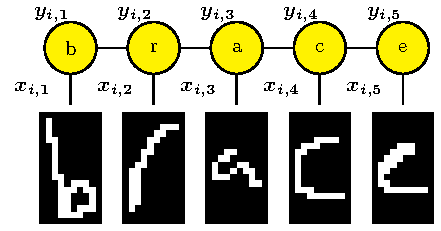
\includegraphics[width=.5\textwidth]{crf}
	\caption[Example of graphical model for the optical character recognition (OCR) task]{
		Example of graphical model for the optical character recognition (OCR) task.
		We want to exploit the structure of the word to predict that $y_{i,5}$ is an "e" and not a "c".
		This can be done by working on the pairs $y_{i,\{t, t+1\} } = (y_{i, t}, y_{i, t+1})$, the cliques of that model.
		}
		\label{crf example}
\end{figure}

\subsection{Primal Problem}
We have a data set $(x_i, y_i)_{i \in [1,n]}$ of $n$ i.i.d. input and structured output pairs.
The parameter is learned by minimizing the $\ell_2$-regularized negative log-likelihood:
\beq\label{negative log-likelihood}
	\min_{\bw \in \real^d} \: \frac{\lambda}{2}\| \bm w\|_2^2 + \frac{1}{n} \sum_{i=1}^{n} -\log\left(p(y_i | x_i ; \bw) \right) \, .
\eeq
We now rewrite it using the notation for the SDCA setup for multi-class classification from~\citet{shalev2016accelerated}.
Denote $M_i = |\cY_i|$ the number of labelings for sequence~$i$.
Denote $A_i$ the $d \times M_i$ matrix whose columns are the \textit{corrected features} $\{\psi_i(y) := F(x_i, y_i) - F(x_i, y)\}_{y \in \cY_i}$.
Denote also $\phi_i(s) := \log \big(\sum_{y \in \cY_i} \exp(s_y)\big)$ the log-partition function for the scores $s \in \real^{M_i}$. The negative log-likelihood can be written $-\log(p(y_i|x_i ;\bm w)) = \phi_i(-A_i^{\top} \bm w)$. The primal objective function to minimize over $\bm w \in \real^d$ thus  becomes:
\begin{equation}
	\label{eq:primal_problem}
	\cP(\bm w) := \frac{\lambda}{2}\| \bm w\|_2^2
	+ \frac{1}{n}   \sum_{i=1}^{n} \phi_i(-A_i^{\top} \bm w) \, .
\end{equation}

\subsection{Dual Formulation}
The above minimization problem~\eqref{eq:primal_problem} has an equivalent {\it Fenchel convex dual} problem \citep{lebanon2002boosting}.
Denote $\Delta_{M}$ the probability simplex over $M$ elements.
Denote $\alpha_i \in \Delta_{M_i}$ the set of dual variables for a given $x_i$.
The dual problem handles directly the probability of the labels for the training set.
The dual objective to maximize over the choice of $\balpha = (\alpha_1, \ldots, \alpha_n) \in \Delta_{|\cY_1|} \times \ldots \times \Delta_{|\cY_n|} $ is:
\begin{equation}
	\label{dual problem}
	\cD(\balpha) := -\frac{\lambda}{2} \| \frac{1}{n \lambda} \sum_i A_i \alpha_i \|^2
	+ \frac{1}{n} \sum_{i=1}^n H(\alpha_i) \, ,
\end{equation}
where $H(\alpha_i) := - \sum_{y \in \cY_i} \alpha_i(y) \log(\alpha_i(y))$ is the entropy of the probability distribution $\alpha_i$. The negative entropy appears as the convex conjugate of the softmax: $-H = \phi^*$.

\subsection{Optimality Conditions}
We define the \emph{conjugate weight} function $\hat{w}$ as follows:
\alignn{
		\hat{w}(\balpha)
		&:= \frac{1}{n \lambda} \sum_i A_i \alpha_i
		= \frac{1}{\lambda n} \sum_{i=1}^n \mathbb{E}_{y \sim \alpha_i} [\psi_i(y)] \\
		&= \frac{1}{\lambda } \left( \frac{1}{ n} \sum_{i=1}^n F(x_i, y_i)
		-  \frac{1}{n} \sum_{i=1}^n \mathbb{E}_{y \sim \alpha_i} [F(x_i, y)] \right) \, .
}
It is the difference between the average of the ground truth features, and the average of the expected features for the dual variable, up to a factor $\frac{1}{\lambda}$.
One can show that $\hat{w}(\balpha^{\star}) = \bm w^{\star}$ where $\bm w^{\star}$ and $\balpha^{\star}$ are respectively the optimal primal parameters and the optimal dual parameters.

We  also  define  \emph{conjugate} probabilities $\hat{\alpha}_i$ as follows:
\begin{equation}
	\forall i, \quad \hat{\alpha}_i(\bm w) := \nabla_s\phi_i(-A_i^{\top} \bm w) = p(.|x_i; \bm w).
	\label{primal to dual}
\end{equation}
We get another optimality condition $\hat{\alpha}(\bm w^{\star}) = \balpha^{\star}$.
These two optimality conditions can be deduced directly from the structure of the duality gaps.

\subsection{Duality Gaps}\label{sec:duality gaps}
Note that $\cP(\bm w ) \geq \cD(\balpha)$ is always true, with equality at the optimum. The {\it duality gap} is defined by:
\beq
	g(\bm w, \balpha) = \cP(\bm w) -\cD(\balpha) \, .
\eeq
%We can write the primal and dual objective with the conjugate variables defined above:
%\beqa
%	\cP(\bm w) & = & \frac{\lambda}{2}\| \bm w\|_2^2
%	+ \frac{1}{n}   \sum_{i=1}^{n} -\log( \hat\alpha_i(w)(y_i) ) \\
%	\cD(\balpha) &=& -\frac{\lambda}{2} \| \hat w (\balpha) \|^2
%	+ \frac{1}{n} \sum_{i=1}^n H(\alpha_i)
%\eeqa
Note that we can rewrite the primal gradient as following:
\begin{equation}\label{primal gradient}
	\nabla \cP (\bw) = \lambda( \bw - \hat{w}\circ \hat{\alpha}(\bm w) ) \, .
\end{equation}
One can verify that:
\beqa
	\label{primal duality gap}
	g( \bm w,\hat{\alpha}(\bm w))
	& = & \frac{\lambda}{2} \|\bm w- \hat{w}(\hat{\alpha}(\bm w))\|^2 \\
	& = &  \frac{1}{2 \lambda} \| \nabla \mathcal P (\bm w) \|^2 \, . \label{eq:gradientGap}
\eeqa
This  structure of the gap for the primal weights and its conjugate dual probabilities have an equivalent in the dual.
Denote the Fenchel duality gap of $\phi_i$ for the scores $s_i = -A_i^T\bw$ and probabilities $\balpha_i$:
\begin{equation} \label{eq:Fench}
	F_i(s_i,\alpha_i) := \phi_i(s_i) + \phi_i^*(\alpha_i) + s_i^T \alpha_i \geq 0.
\end{equation}
The positivity comes from the definition of convex conjugates.
The gap is zero when $s_i$ and $\alpha_i$ are conjugate variables for $\phi_i$, e.g. $\alpha_i = \nabla \phi_i(s_i)$.
For any smooth loss~$\phi_i$, the duality gap between $\hat{w}(\balpha)$ and $\balpha$ decomposes as a sum of Fenchel gaps \citep{shalev-shwartz_accelerated_2013-1}:
\beqa
	\label{eq:Fench_blocks}
	g(\hat{w}(\balpha), \balpha)
	& = &\frac{1}{n} \sum_i F( -A_i^T \hat w (\balpha), \alpha_i).
\eeqa
The log-sum-exp and the entropy are a special pair of conjugates.
Their Fenchel duality gap is also equal to the Bregman divergence generated by $\phi_i^*=-H$, the Kullback-Leibler divergence: $F_i(s_i ,\alpha_i) = D_{KL}(\alpha_i || \nabla\phi_i(s_i) )$. Writing this for the same pair of conjugate variables yields:
\beqa
	\label{dual duality gaps}
	g(\hat{w}(\balpha), \balpha)
	& = &\frac{1}{n} \sum_i D_{KL} (\alpha_i || \hat{ \alpha}_i(\hat{w}( \balpha)).
\eeqa
The duality gaps~\eqref{primal duality gap}  and~\eqref{dual duality gaps} are typically used to monitor the optimization.
In Appendix~\ref{app:bound duality gap}, we explain how one can transfer a convergence guarantee on the primal or dual suboptimality to a convergence guarantee on the duality gap.\footnote{
    This implies that convergence results on the dual problem directly translates to convergence results on the primal and vice-versa;
     a fact apparently missed in the linear rate comparison of~\citet{schmidt2015non}.
}
Moreover, the block-separability of gaps from~\eqref{dual duality gaps} can motivate an adaptive sampling scheme, as we describe in Section~\ref{Adaptive Sampling}.

\subsection{Interpretation}
The primal formulation chooses a $\bm{w}$ of small norm so as to maximise the conditional probability of observing the labels.
Conversely, the  dual formulation chooses conditional probabilities of the labels so as to minimize the $\ell_2$ distance between the expected features and empirical expectation of the ground truth features.
The optimal distribution would be the empirical  distribution, if not for the entropic regularization that favors more uniform probabilities.
This is the regularized version of the classical duality between maximum-likelihood and maximum-entropy for exponential families.

The optimality conditions show that the solution of the primal Problem~\eqref{eq:primal_problem} is also a \emph{fixed point} for the function~$\hat w \circ \hat \alpha$.
Because of the gradient form~\eqref{primal gradient}, the gradient descent update can also be written as a \emph{relaxed} fixed point update:
\begin{align}
		\bw^+
		& = \bw - \gamma \nabla \cP(\bw) \\
		& = (1-\gamma \lambda) \bw  + \gamma \lambda \,\, \hat w \circ \hat \alpha (\bw) \, .
\end{align}
The algorithm SDCA described in the next section also admits a relaxed fixed point update on the block $\alpha_i$ (see~\eqref{eq:dual_fixed_pt_update}).
More generally, optimization algorithms for Problem~\eqref{eq:primal_problem} can often be interpreted as a back and forth between the conjugate variables $w$ and $\hat w(\hat \alpha(\bm w))$ (primal methods) or $\alpha$ and $\hat \alpha(\hat w( \balpha))$ (dual methods).
For instance, one could interpret OEG as a relaxed fixed point iteration over the score variables $s_i = -A_i^T\bw$.
\begin{displaymath}
    \xymatrix{
    	\bm w \ar[r]^-{\hat{\alpha}}
    	&   \left( \nabla_s \phi_i(-A_i^T \bm w) \right)_{i=1}^n \ar[d] \\
		\frac{1}{n \lambda} \sum_i A_i \alpha_i  \ar[u]
		&  \balpha \ar[l]_-{\hat{w}}
	}
\end{displaymath}
Most of the results presented in this section and in Section~\ref{Adaptive Sampling} can be transposed to other kinds of loss and regularization, under some regularity assumptions.
Our focus in this paper is the application of SDCA to CRF models and thus we focused the discussion on the log-likelihood setting and the $\ell_2$ norm, which are widely used.


%%%%%%%%%%%%%%%%%%%%%%%%%%%%%%%%%%%%%%%%%%%%%%%%%%%%
\section{Proximal Stochastic Dual Coordinate Ascent} \label{sec:SDCA}

We first describe the SDCA in its general setting, and then describe the necessary modifications for training a CRF.

\subsection{General Setting}
The stochastic dual coordinate ascent algorithm (SDCA) updates one dual coordinate at a time so as to maximize the dual objective.
SDCA was originally proposed for binary classification~\citep{shalev-shwartz_stochastic_2013} where each dual variable~$\alpha_i$ lives in $\Delta_2 = [0,1]$.
In this case, it is possible to do exact coordinate maximization of the dual objective over a single $\alpha_i$ with standard one dimensional optimization.

In the multi-class setting however, there is no simple way to maximize the dual objective over the block $\alpha_i \in \Delta_K$.
The algorithm with the surprising name of Proximal-SDCA\footnote{We simply call it SDCA in the rest of this paper}, option II~\citep{shalev2016accelerated} proposes a solution to this problem.
It updates $\alpha_i$  in a clever direction derived from the primal-dual relationship, which amounts to a relaxed fixed point update. See Algorithm~\ref{sdca general}.

\begin{algorithm}[t]
    \caption{Prox-SDCA (option II) called SDCA here}%
    \label{sdca general}
	\begin{algorithmic}
        %
        \STATE Initialize $\alpha_i^{(0)} \in \Delta_{M_i}, \forall i$
        \STATE Let $\bw^{(0)} = \hat{w}(\bm{\alpha}^{(0)}) = \frac{1}{\lambda n} \sum_i A_i \alpha_i$
        %
       \FOR{$t=0, 1\dots$}
                \STATE Sample $i$ uniformly at random in $\{1,\ldots,n\}$
                \STATE Let $ \beta_i := \hat{\alpha}_i(\bw) = \nabla_s \phi(-A_i^T \bw)$
                \STATE Let $\delta_i = \beta_i - \alpha_i^{(t)}$ \COMMENT{dual ascent direction}
                \STATE Let $\bv_i = \frac{1}{\lambda n} A_i \delta_i $ \COMMENT{primal direction}
                \STATE Solve Equation~\eqref{line search equation} to get $\gamma^*$ \COMMENT{Line Search}
               \STATE Update $\alpha_i^{(t+1)} := \alpha_i^{(t)} + \gamma^* \delta_i$
               \STATE Update $\bw^{(t+1)} := \hat{w}(\bm{\alpha}^{(t+1)}) = \bw^{(t)} + \gamma^* \bv_i $
        \ENDFOR
	\end{algorithmic}
\end{algorithm}


We now describe the idea.
At all time, we maintain the pair of dual and primal variables~$(\balpha, \bw = \hat w (\balpha))$.
At each step, we sample a training point~$i$.
We compute $\beta_i = \nabla_s \phi_i(-A_i^T \bw) = \hat \alpha_i \circ \hat w(\balpha)$,  the next fixed point iterate.
We then define the dual ascent direction by $\delta_i := \beta_i - \alpha_i$.
Finally we update the block~$\alpha_i$ with the right step size so as to increase the dual objective~$\cD(\balpha)$ using a relaxed fixed point update:
\begin{equation} \label{eq:dual_fixed_pt_update}
	\alpha_i^+ \leftarrow \alpha_i + \gamma \delta_i = (1-\gamma)\alpha_i + \gamma \hat \alpha_i \circ \hat w(\balpha) \, .
\end{equation}
The dual ascent direction is guaranteed to increase $\cD(\balpha)$, unless $\delta_i = 0$ (this actually means that the block is already optimal, see~\eqref{dual duality gaps}).
The primal weights $\bw = \hat w (\balpha)$ are related to $\balpha$ by a linear transformation.
Define the primal direction $\bv_i = \frac{1}{\lambda n} A_i \delta_i \in \real^d$.
One can update the weights directly: $\bw^+ \leftarrow \bw + \gamma \bv_i$.

The step size $\gamma \in [0,1]$  is either fixed, or found via line search.
In practice the fixed step size for which convergence is guaranteed is really small.
The line search is relatively cheap as we are looking at only one block:
\begin{equation}\label{line search equation}
	\gamma^*
	:= \argmax_{\gamma \in [0,1]} - \phi^*_i(\alpha_i + \gamma \delta_i)
	- \frac{\lambda n}{2} \| \bw + \gamma \bv_i \|^2.
\end{equation}
Note that one can decompose the quadratic term and precompute $ \langle \bw, \bv_i \rangle$ and $\| \bv_i \|^2 $ to accelerate the optimization.
The bottleneck remains the computation of $\phi^*_i$ (and its derivatives).




\subsection{Adaptation to CRF}
In the CRF setting, the dual variable~$\alpha_i$ is exponentially large in the input size~$x_i$.
For a sequence $x_i$ of length $T$ where each node can take up to $K$ values, the number of possible labels is $M_i = |\cY_i | = K^{T}$.
It might not even fit in memory.
Instead, the standard approach used in OEG and SAG is to consider the marginal probabilities $(\mu_C)_{C \in \cC}$ on the cliques of the graphical model.
Similarly, we replace $\balpha$ by $\bmu = (\mu_1, \cdots, \mu_n)$, where $\mu_i \in \prod_C \Delta_{C}$ is the concatenation of all the clique marginal vectors for the sample $i$.
For the same sequence $x_i$, this reduces the memory cost to $K^2(T-1)$ for the pair marginals.
We denote $m_i= \sum_C |\cY_{i, C} |$ this new memory fingerprint.
For a sequence long enough, we have $m_i \ll M_i$.
The associated weight vector can still be expressed as function of $\bmu$ thanks to the separability of the features:
\begin{equation}
	\label{weights from marginals}
	\hat w (\bmu) = \frac{1}{\lambda n} \sum_i \sum_C \mathbb E_{\mu_{i, C}}[\psi_{i, C}]
	= \frac{1}{\lambda n} \sum_i B_i \mu_i,
\end{equation}
where $B_i = (\psi_{i,C}(y_{C}) )_{C, y_C} \in \real^{d \times m_i}$ is the horizontal concatenation of the cliques feature vectors.

\begin{algorithm}[t]
    \caption{SDCA for CRF}%
    \label{sdca for crf}
	\begin{algorithmic}
        %
        \STATE Initialize $\mu_{i}^{(0)} \in \prod_C \Delta_{C}$ consistently $\forall i$ \COMMENT{use~\eqref{eq:initialization}}
        \STATE Set $\bm{w}^{(0)}  :=  \hat{w}(\bm\mu^{(0)}) = \frac{1}{\lambda n} \sum_i B_i \mu_i^{(0)}$ \,\, \COMMENT{See \eqref{weights from marginals}}
        \STATE (Optional) Let $\quad g_i = 100, \forall i $
        %
       \FOR{$t=0, 1\dots$}
                \STATE Sample $i$ uniformly at random in $\{1,\ldots,n\}$
                \STATE (Alternatively)  Sample $i$ proportionally to $g_i$
                \STATE Let $\nu_{i, C} (y_C) := p(y_C | x_i; \bw^{(t)}), \forall C\in\cC$  \COMMENT{\textbf{oracle}}
                %
                \STATE (Optional) Let $g_i = \tilde D(\mu_i || \nu_i)$  \COMMENT{duality gap \eqref{divergence marginal}}
                \STATE Let $\delta_i = \nu_i - \mu_i^{(t)}$ \COMMENT{ascent direction}
                \STATE Let $\bv_i = \frac{1}{\lambda n} \hat w(\delta_i)$ \COMMENT{primal direction}
                \STATE Solve Equation~\eqref{crf line search} to get $\gamma^*$  \COMMENT{Line Search}
                %
               \STATE Update $\mu_i^{(t+1)} := \mu_i^{(t)} + \gamma^* \delta_i$
               \STATE Update $\bm{w}^{(t+1)} := \hat{w}(\bm\mu^{(t+1)}) = \bm{w}^{(t)} + \gamma^* \bv_i $
        \ENDFOR
	\end{algorithmic}
\end{algorithm}

Now, assume that the graph has a {\it junction tree} structure $T=(\cC,\cS)$~\citep[Def.~10.3]{koller2009PGM}, where $\cC$ is the set of maximal cliques and $\cS$ the set of separators.
We can then run message passing on the junction tree to infer the new marginals given weights $\bw$: $\hat \mu_i(\bm w) = {p(y_C=. | x_i ;\bw)}$.
We can also now recover the joint probability $\alpha_i(y)$ as a function of its marginals $\mu_{i, C}$ \citep[Def.~10.6]{koller2009PGM}:
\begin{equation}
	\label{joint from marginals}
	\alpha_i(y) = \frac{\prod_{C\in\cC} \mu_{i, C} (y_C)}{\prod_{S \in\cS} \mu_{i, S}(y_S)}.
\end{equation}


Equation~\eqref{joint from marginals} in turn allows us to compute the entropy and the divergences of the joints, using only the marginals. Let $\mu_i$ and $\nu_i$ be the marginals of respectively $\alpha_i$ and $\beta_i$, then the entropy and the Kullback-Leibler divergence are given by:
\begin{equation}
	\label{entropy marginal}
	\tilde H (\mu_i)
	:= H (\alpha_i)
	= \sum_C H(\mu_{i, C}) - \sum_S H(\mu_{i, S})
\end{equation}
and
\alignn{
	\label{divergence marginal}
 	\tilde D (\mu_i || \nu_i)
 	:=D_{KL}(\alpha_i|| \beta_i)
 	= \sum_C D_{KL}(\mu_{i, C}||\nu_{i,C}) - \sum_S D_{KL}(\mu_{i, S}||\nu_{i, S}). 
}

With this expression of the entropy~\eqref{entropy marginal}, we can compute the dual objective, and thus perform the line search:
\begin{equation}\label{crf line search}
	\gamma^* = \argmax_{\gamma \in [0,1]} \tilde H(\mu_i^{(t)} + \gamma \delta_i) - \frac{\lambda n}{2} \| \bw^{(t)} + \gamma \bv_i \|^2.
\end{equation}
With the Kullback-Leibler divergence~\eqref{divergence marginal}, we can compute efficiently the individual duality gaps from~\eqref{dual duality gaps}.
Algorithm~\ref{sdca for crf} describes this variation of SDCA, with as an option a non-uniform sampling strategy defined in  Section~\ref{ssec:gap_sampling}.

%%%%%%%%%%%%%%%%%%%%%%%%%%%%%%%%%%%%%%%%%%%%%%%%%%%%
\section{Implementation} \label{sec:implementation}
We provide in Appendix~\ref{app:sec:implementation} a discussion of various important implementation aspects summarized here.
\begin{compactenum}
\item The initialization of dual methods for CRFs can significantly influence their performance. As explained in Appendix~\ref{app:sec:implementation}, we use: 
\begin{equation} \label{eq:initialization}
	\balpha^{(0)} := \varepsilon \bu + (1-\varepsilon) \bm\delta \, ,
\end{equation}
where $\bu$ is the uniform distribution on each block, $\bm\delta$ is a unit mass on each ground truth label and $\varepsilon$ is a small number.
\item Storing the dual variable may be expensive and one should allocate a decent amount of memory.
\item The line search requires computing the entropy of the marginals.
This is costly and we used Newton-Raphson algorithm to minimize the number of iterations.
This in turn requires storing the logarithm of the dual variable.
\end{compactenum}
%%%%%%%%%%%%%%%%%%%%%%%%%%%%%%%%%%%%%%%%%%%%%%%%%%%%
\section{Adaptive Sampling for SDCA} \label{Adaptive Sampling}

Recently, there has been a lot of attention on non-uniform sampling for stochastic methods.
The general goal is to sample more often points which are harder to classify and can bring more progress on the objective.
These methods are said to be \textit{adaptive} when the sampling probability changes during the optimization.
SDCA itself has had several adaptive schemes proposed.
In the following, we attempt to explain and relate these methods, and suggest new schemes that work well on our problem.

\subsection{Ascent Lemma}\label{ascent lemma}
We start by restating the ascent lemma from Equation~(25) in \citet{shalev-shwartz_accelerated_2013-1}.
This lemma inspires and supports all the strategies.

\paragraph{Ascent after sampling $i$:}
At iteration $t$, if we sample $i$ and take a step of size  $\gamma_i \in [0,1]$, we can lower bound the resulting dual improvement:
\begin{align}
	\label{one point descent}
    & n (\cD(\balpha^+) - \cD(\balpha)) \notag \\
    & \geq \gamma_i \underbrace{ \big [ \phi(-A_i^T \bw) + \phi^*(\alpha_i) + \bw^T A_i \alpha_i \big ] }
    _{ \textrm{Fenchel gap} =: g_i} 
    + \gamma_i \bigg ( \frac{(1-\gamma_i)}{2} - \frac{\gamma_i R_i}{2 \lambda n} \bigg )\| \beta_i - \alpha_i \|^2_1
\end{align}
where  $R_i := \|A_i\|^2_{1\rightarrow 2}  = \max_{y\in\cY_i} \| \psi_i(y) \|_2^2 $ is the squared radius of the corrected features for sample $i$.

Note that compared to the original text, we used the fact that the regularizer is the $\ell_2$ norm and the loss is $1$-smooth with respect to the $\ell_\infty$ norm.
We define $R:=\max_i R_i$, ${\bar R := \frac{1}{n} \sum_i R_i}$ and $\bar g := \frac{1}{n} \sum_i g_i$ the true duality gap (see~\eqref{eq:Fench}-\eqref{eq:Fench_blocks}).
We also introduce $L_i := \lambda + \frac{R_i}{n}$ an upper bound on the smoothness of loss $i$ plus regularizer for the $\ell_2$ norm.
We recall from Section~\ref{sec:duality gaps} that $g_i = D_{KL}(\alpha_i || \beta_i)$~\eqref{dual duality gaps}.
We give the name \textit{residual} to $d_i := \| \beta_i - \alpha_i \|^2_1$.

This lemma is derived with standard assumptions and inequalities on the smoothness of the loss and the strong convexity of the regularizer.
The first term of the lower bound is the ascent guarantee while the other term gives condition on the step-size to ensure progress.
We refer the reader to the original paper for more details.

To get the expected progress (conditioned on the past) after sampling with probability $\bm p$, we simply need to take the sum of the inequality above after multiplying both sides by $p_i$.
Our goal is to maximize this lower bound by choosing the right probability $\bm p$ and step sizes $\bm \gamma$.
To be able to conclude the proof with the original method, we also want some constants time the duality gap $\bar g$ to appear in the lower bound -- the gap is lower bounded by the dual suboptimality and thus this constant will give the linear rate of convergence.
The lemma can then transpose this result from the dual sub-optimality to the duality gap as described in Appendix~\ref{app:bound duality gap}.
From there on there are two general approaches: importance sampling and duality gap sampling.

\subsection{Importance and Residual Sampling}
With the importance sampling approach, the goal is to set the step-size and the probability so that they cancel each other out: $\gamma_i = \frac{\gamma}{p_i}$.
One then get an unbiased estimate of the true duality gap from~\eqref{dual duality gaps} as the first  term of the upper bound.
What is left is maximizing the second term with respect to $\bm p$.
This is the approach proposed by \citet{Zhao2015StochasticOptimizationImportance} (Importance Sampling, left term below) and generalized by \citet{csiba2015stochastic} (Residual sampling, a.k.a. AdaSDCA for binary classification, right term):
\begin{equation}
		p_i \propto L_i \quad \text{or} \quad p_i \propto d_i \sqrt{L_i}.
\end{equation}
These sampling schemes somehow allow to maximize the second term of~\eqref{one point descent}.
Intuitively, they replace a dependency on $R$ in the convergence rate by a dependency on $\bar R$.
They can give good results on binary and multi-class logistic regression. There are a few issues though.
\vspace{-\topsep}
\begin{itemize}
    \setlength{\parskip}{0pt}
    \setlength{\itemsep}{3pt plus 1pt}
    \item One needs an accurate estimate of the $L_i$.
    \item Importance sampling is not adaptive.
    \item In the CRF setting, the residual is $d_i = \| \beta_i -\alpha_i \|_1^2$.
    It is the squared $\ell^1$ norm of a vector of exponential size.
    We are not aware of any trick to compute it efficiently.
\end{itemize}
\vspace{-\topsep}

\subsection{Gap Sampling}\label{ssec:gap_sampling}
To make sure that the second term is positive, the original proof of uniform SDCA sets  $\gamma_i = \gamma = {(1+ \frac{R}{\lambda n})^{-1}}$ to obtain:
\begin{equation}
		n \mathbb E_p[D(\balpha^+) - D(\balpha)]
		\geq \gamma \sum_i p_i g_i.
\end{equation}
Assuming a full knowledge of the duality gaps $g_i$, the optimal decision is to sample the point with maximum duality gap.
This was done by \citet{dunner2017efficient} in the context of multi-class classification on a pair CPU-GPU. While the GPU computes the update, the CPU updates as many duality gaps as possible.
This lead to impressive acceleration over massive datasets.

However, this is not our current setting.
We know and update only one gap at a time (for efficiency).
Because of staleness of the gaps, our experiments with this method did not even converge for the most part (see Section~\ref{experiment sampling}).
We need a more robust method.

We take inspiration from what was done by \citet{osokin2016minding} to improve the Block-Coordinate Frank-Wolfe (BCFW) algorithm \citep{lacoste2013block}.
We propose to bias sampling towards examples whose duality gaps are large: $p_i \propto g_i$.
If we know all the duality gaps, the expected improvement reads:
\begin{equation}
	n \mathbb E_p[D(\balpha^+) - D(\balpha)]
		\geq \chi(\bm g)^2 \, \gamma \, \bar g,
\end{equation}
where $	\chi(\bm g) = \sqrt{ \frac{ \frac{1}{n} \sum_i g_i^2}{\bar g^2} } \in [1, \sqrt n] $ is the non-uniformity of the duality gaps, as defined in \citet[Section 3.1]{osokin2016minding}.
The value $\chi(\bm g)^2 \gamma$ is the value that will appear in the linear convergence rate of this method.
It means that the convergence rate for gap sampling \textbf{dominates} the one for uniform sampling.
This is different from what was observed for  BCFW where they could not prove dominance in general.

In practice we use stale estimates of the gaps and there are no convergence guarantees.
We discuss more this issue in section \ref{experiment sampling}.

We also explored a combination of gap sampling and importance sampling.
We could get similar convergence rate where a trade-off appeared between the mean smoothness and the non-uniformity.
We detail these considerations as a technical report in Appendix \ref{app:nusampling} for the interested reader.

%%%%%%%%%%%%%%%%%%%%%%%%%%%%%%%%%%%%%%%%%%%%%%%%%%%%
\section{Experiments} \label{sec:experiments}
We conducted these experiments to answer three questions:
(1) How does the line search influence SDCA?
(2) How do the non-uniform sampling schemes compare with each other?
and (3) How does SDCA compare with SAG and OEG on sequence prediction?

\subsection{Experimental Setting}

We applied the experimental setup outlined by \citet{schmidt2015non}.
We implemented SDCA to train a classifier on four CRF training tasks: (1) the optical character recognition (OCR) dataset~\citep{taskar2004max}, (2) the CoNLL-2000 shallow parse chunking dataset (CONLL), (3) the CoNLL-2002 Dutch named-entity recognition dataset (NER), and (4) a part-of-speech (POS) tagging task using the Penn Treebank Wall Street Journal data.
Additional details regarding these datasets are provided in Table~\ref{datasets summary}.
Note that the tasks (2), (3), (4) are about language understanding.
They use sparse features (the ratio $a/A$ from the table is small).
The sparsest data set is NER.
Note that POS is considerably larger than other datasets.
All experiments are performed with a regularization factor $\lambda=1/n$.
We used our own implementation\footnote{The code to reproduce our experiments is available at: \url{https://remilepriol.github.io/research/sdca4crf.html}.} of SDCA coded in plain Python and Numpy \citep{walt2011numpy}.
In most plots we report the logarithm base 10 of the primal sub-optimality.
We got the optimum by running L-BFGS a large number of iterations.

\begin{table}[t]
	\centering
	\caption[Summary of the datasets we used in our experiments]{
	Dataset summary.
	$d$ is the dimension of $\bw$.
	$n$ is the number of data points (sequences).
	$N$ is the number of nodes (e.g. sum of sequences length).
	$K$ is the number of possible labels for each node.
	$A$ is the number of attributes (see Appendix~\ref{app:feature}).
	$a$ is the maximum number of attributes extracted from one node.
	Mem. is the memory required by the pairwise marginals stored as float 64.
	The pairwise marginals dominate the memory cost.
	}
	\label{datasets summary}
	{\small
		\begin{tabular}{lllll}
			\toprule
			Dataset          &   OCR  &   CONLL   &    NER   &      POS \\
			\midrule
			$d$ &   \convert{4082} &   \convert{1643026} &  \convert{2798955} &  \convert{8572770} \\
			$n$ &   \convert{6202} &      \convert{8936} &    \convert{15806} &    \convert{38219} \\
			$N$ &  \convert{52827} &    \convert{211727} &   \convert{202931} &   \convert{912273} \\
			$K$ &     26 &        22 &        9 &       45 \\
			$A$ &    128 &     \convert{74658} &   \convert{310983} &   \convert{190458} \\
			$a$ &    128 &        19 &       20 &       13 \\
			Mem.(GiB)      &    0.2 &       0.7 &      0.1 &       13 \\
			\bottomrule
		\end{tabular}
	}
\end{table}


\subsection{Influence of the Line Search}\label{experiment line search}

We implemented the safe bounded Newton-Raphson method from \citet[Section 9.4]{press_numerical_1992} on the derivative of the line search function.
A natural question to ask is : how precise should the line search be?
The stopping criterion for this algorithm is the size of the last step taken so there is no proper precision parameter.
We refer to this stopping criterion for the line search as the sub-precision of SDCA.

We discovered experimentally that the convergence of SDCA is mostly  independent of the sub-precision.
On all datasets, if we ask 0.01 sub-precision or less, SDCA converges with the same rate.
An explanation is that the accuracy of the optimization arises from iterates $\balpha$ and $\hat \alpha(\hat w(\balpha))$ getting closer to each other in the simplex with each iteration.

Reaching 0.01 or 0.001 takes on average 2 iterations.
Each iteration of Newton's method require the computation of the first and second derivative of the line search objective~\eqref{crf line search}.
In the following we report results with sub-precision 0.001 to be on the safe side.
These 2 iterations were taking about 30\% of the algorithms running time for each dataset.\footnote{
We also tried initializing the line search with 0.5 or with the previous step size.
There was no significant difference.
}

We also performed experiments with only one step of the Newton update.
The convergence was not affected on OCR, CONLL and POS, but convergence failed on NER (see Figure~\ref{fig:subprecision} of Appendix~\ref{app:comp_plots}).
This phenomenon could be related to sparsity.

\subsection{Comparison of Sampling Schemes} \label{experiment sampling}
We compare the performance of four sampling strategies with 20\% of uniform sampling against the full Uniform approach, on the OCR dataset (see results in Figure~\ref{fig:comparison sampling schemes}):\vspace{-2mm}
\begin{itemize}
  \item \textit{Importance:} sample proportionally to the smoothness constants $L_i = \lambda +\frac{R_i}{n}$. We report how we evaluated the radii $R_i$ in Appendix \ref{app:radius}. \vspace{-2mm}
  \item \textit{Gap:} sample proportionally to our current estimate of the duality gaps.\footnote{
  For the gap approaches, we initialize the gap estimates with large values (100) so as to perform a pass over the whole dataset before starting to sample proportionally to the stale estimates.
  } \vspace{-2mm}
  \item \textit{Gap $\times$ importance:} sample proportionally to the product of the gap and smoothness constants. \vspace{-2mm}
  \item \textit{Max:} sample deterministically the variable with the largest recorded gap \citep{dunner2017efficient}.
\end{itemize}
\begin{figure}[t]
\centering 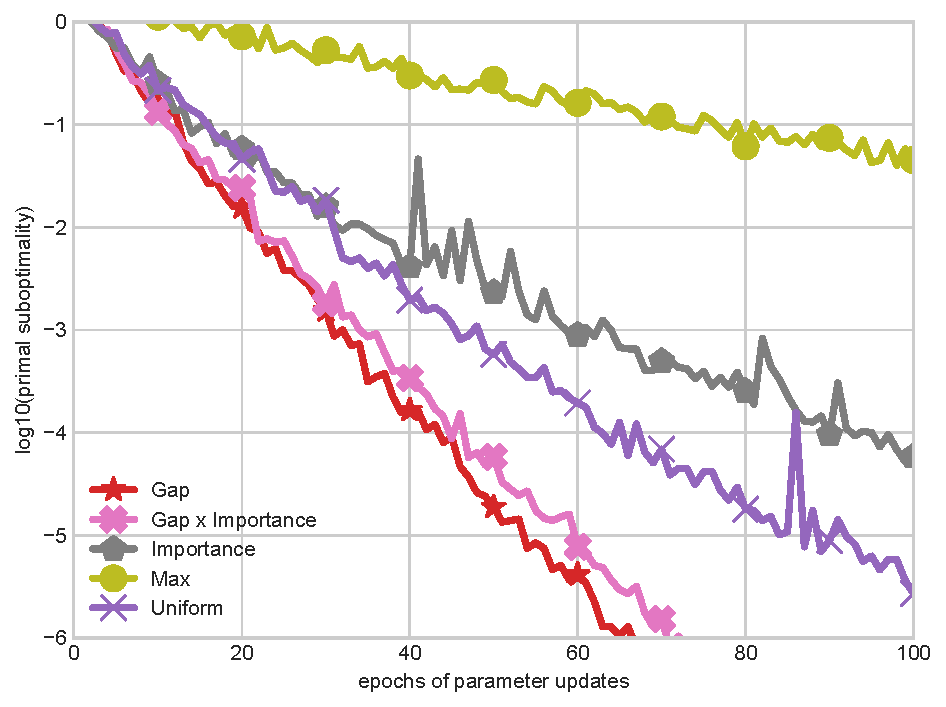
\includegraphics[width=.5\textwidth]{sampling_ocr}
\caption[
	Performance of competing sampling schemes on the OCR dataset 
]{
	Performance of competing sampling schemes on the OCR dataset with 80\% of non-uniformity. Sampling proportionally to the gap gives the best performance.
}
\label{fig:comparison sampling schemes}
\end{figure}

As discussed in Section~\ref{ssec:gap_sampling}, Max sampling is not robust enough to the staleness of the gap estimates and fails to converge here.
We also observe that Importance performs worse than Uniform, and that Gap $\times$ Importance performs worse than Gap.
This  indicates that the smoothness upper bounds we estimated are not informative of the  difficulty of optimizing a point for SDCA.
Overall, Gap sampling  gives the best performance and this is what we use in the following experiments.

The ratio of uniform sampling is here to mitigate the fact that we sample proportionally to stale gaps.
This is the strategy adopted by SAG-NUS~\citep{schmidt2015non} which samples uniformly half of the time.
Another strategy used by~\citet{osokin2016minding} is to update all the duality gaps at once every 10 epochs or so.
Our experiments indicate that these strategies are not needed for SDCA-GAP.
Increasing the ratio of non-uniformity up to 1 only improves the performance on all datasets, though after 0.8 the improvements are marginal, as illustrated by Figure~\ref{fig:non-uniformity} for the NER dataset.
\begin{figure}[t]
\centering 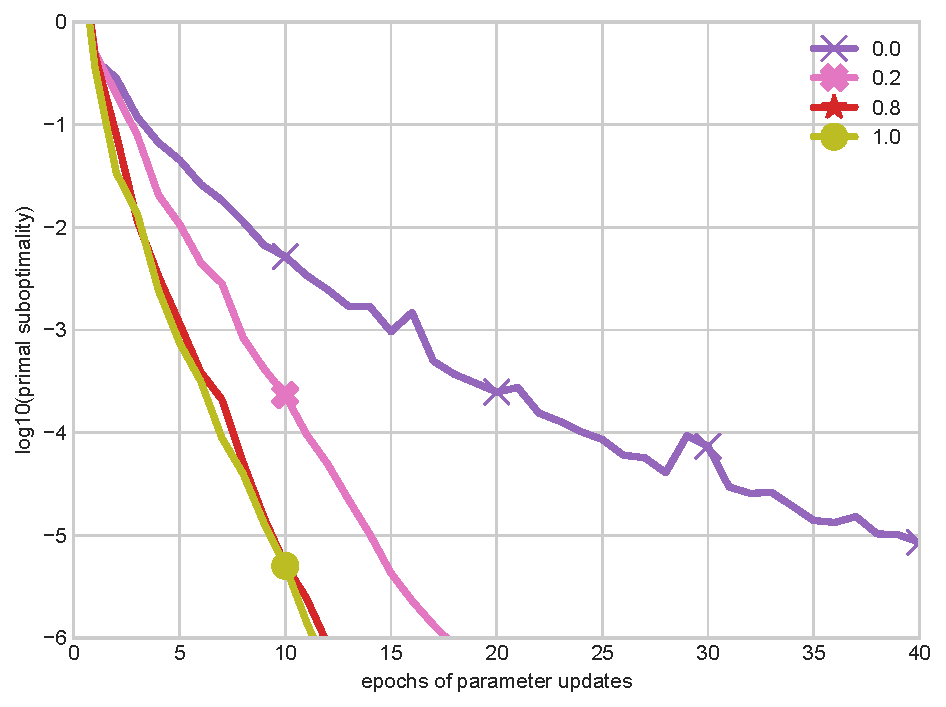
\includegraphics[width=.5\textwidth]{nus_ner}
\caption[SDCA with Gap sampling applied on NER]{SDCA with Gap sampling applied on NER with various fractions of non-uniform sampling, as indicated by the number in the legend.
Increasing the fraction only improves the performance, up to a certain point.}
\label{fig:non-uniformity}
\end{figure}

In fact, the estimate of the total gap maintained by SDCA is somewhat accurate, as illustrated for different datasets in Figure~\ref{fig:ratio} of Appendix~\ref{app:comp_plots}.
Empirically, it always remains within a factor 2 of the true duality gap.
This accuracy is a good news because one can use this estimate of the duality gap as a stopping criterion for the whole algorithm.
Once it reaches a certain precision threshold, one just has to perform one last batch update to check the real value.
This is similar in spirit to SAG, which uses the norm of its estimate of the true gradient as a stopping criterion.
Both are duality gaps estimators (see Equation~\eqref{primal duality gap}).


\subsection{Comparison against SAG and OEG}

We downloaded the code for OEG and SAG-NUS as implemented by~\citet{schmidt2015non} from the SAG4CRF project page.\footnote{\url{https://www.cs.ubc.ca/~schmidtm/Software/SAG4CRF.html}}
We used our own implementation of SDCA with a line search sub-precision of $0.001$.
We provide the comparison in Figure~\ref{fig:comparison with SAG and OEG} according to two different measures of complexity which are implementation independent.

\begin{figure}[t]
\centering
\begin{subfigure}{0.33\linewidth}
\centering
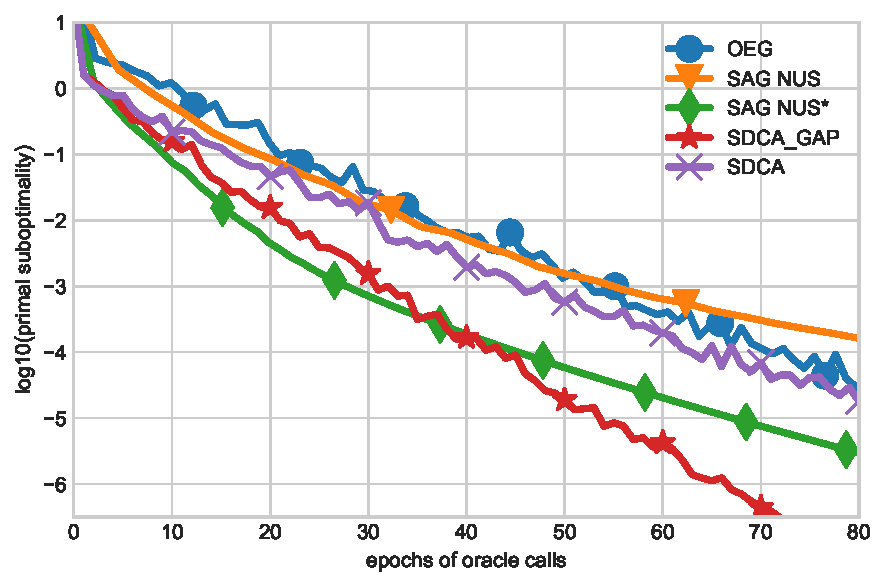
\includegraphics[width=\linewidth]{ocr/primal_calls}
\caption{OCR (Oracle Calls)}\label{fig:OCR oracles}
\end{subfigure}%
\begin{subfigure}{0.33\linewidth}
\centering
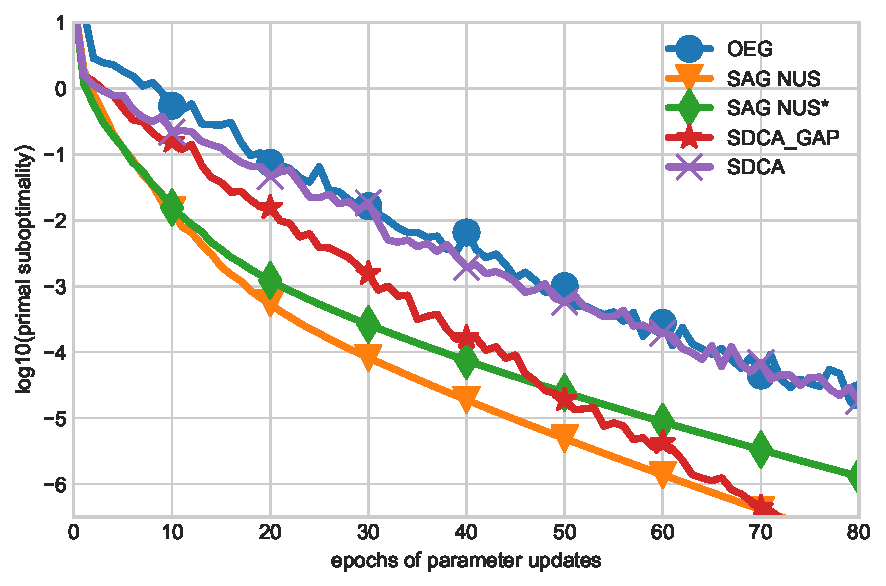
\includegraphics[width=\linewidth]{ocr/primal_iter}
\caption{OCR}\label{fig:OCR}
\end{subfigure}%
\begin{subfigure}{0.33\linewidth}
\centering
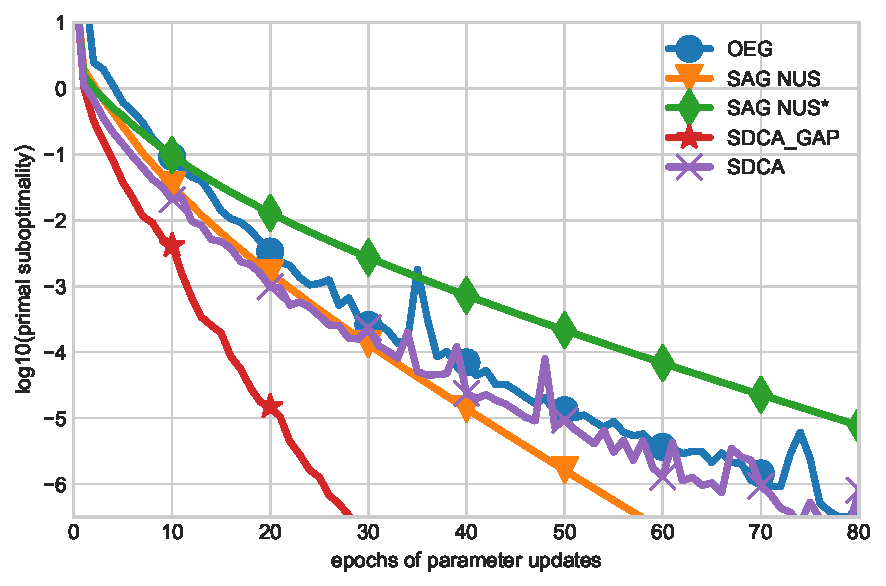
\includegraphics[width=\linewidth]{conll/primal_iter}
\caption{CONLL}\label{fig:CONLL}
\end{subfigure} \\
\begin{subfigure}{0.33\linewidth}
\centering
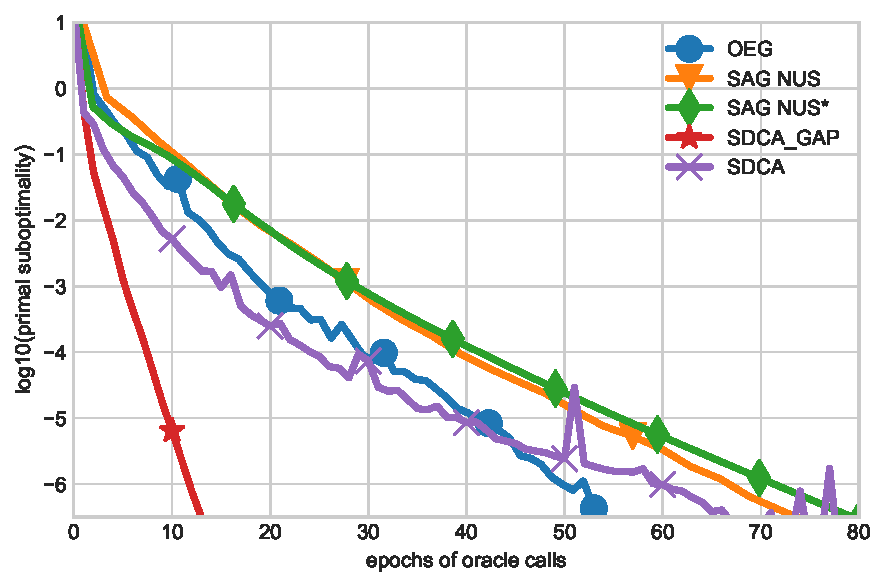
\includegraphics[width=\linewidth]{ner/primal_calls}
\caption{NER (Oracle calls)}\label{fig:NER oracles}
\end{subfigure}%
\begin{subfigure}{0.33\linewidth}
\centering
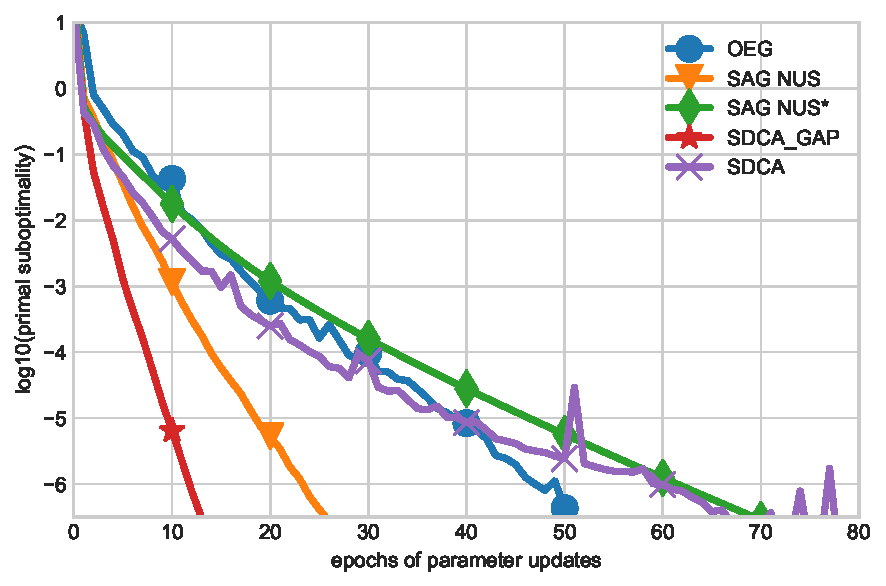
\includegraphics[width=\linewidth]{ner/primal_iter}
\caption{NER}\label{fig:NER}
\end{subfigure}%
\begin{subfigure}{0.33\linewidth}
\centering
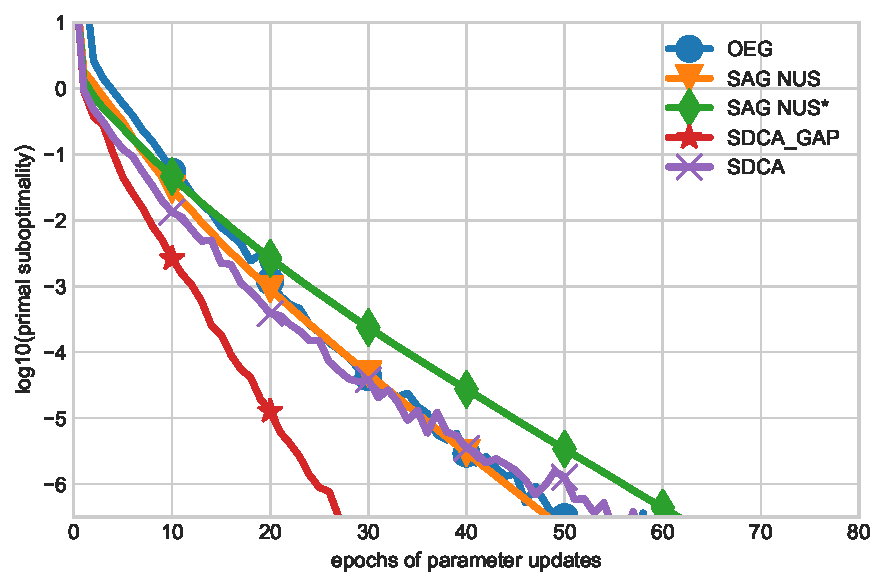
\includegraphics[width=\linewidth]{pos/primal_iter}
\caption{POS}\label{fig:POS}
\end{subfigure}%
\caption[Comparison of SDCA, SAG and OEG on 4 datasets]{Primal sub-optimality as a function of the number of oracle calls (left) or parameters updates (center and right).
	SDCA refers to uniform sampling.
	SDCA-GAP refers to sampling Gap sampling 80\% of the time.
	SAG-NUS performs a line search at every iteration.
	SAG-NUS* implements a line-search skipping strategy.
	It appears worse than SAG-NUS when we look at the number of updates, which hides the cost of the line search.
}
\label{fig:comparison with SAG and OEG}
\end{figure}

\paragraph{Oracle calls.}
\citet{schmidt2015non} compared the algorithms on the basis of the number of oracle calls.
We report these on OCR and NER in Figures~\ref{fig:OCR oracles} and~\ref{fig:NER oracles}.
Results on the other datasets are in Figure~\ref{fig:oracle_calls} in Appendix~\ref{app:comp_plots}.
This metric was suitable for the methods they compared.
Both OEG and SAG-NUS use a line search where they call an oracle on each step.
SDCA does not need the oracle to perform its line search.
However the oracle is message passing on a junction tree.
It has a cost proportional to the size of the marginals.
Each iteration of the line search require computing the entropy of these marginals, or their derivatives.
These costs are roughly the same.
Comparing the number of oracle calls for each method is thus unfairly advantaging SDCA by hiding the cost of its line search.
It becomes a relevant comparison when a marginalization oracle becomes much more expensive than approximating the entropy (see the discussion in Section~\ref{sec:discussion}).
When this cost is hidden, SDCA-GAP is on par with SAG-NUS* on OCR and it is much faster on the sparse datasets.

\paragraph{Parameter updates.}
To give a different perspective, we report the log of the sub-optimality against the number of parameter updates in Figures~\ref{fig:OCR}, \ref{fig:CONLL}, \ref{fig:NER} and~\ref{fig:POS}.
This removes the additional cost of the line search for all methods.\footnote{
This is a penalty for SAG-NUS* which enforces a line-search skipping strategy.
}

We observe that uniform SDCA and OEG need roughly the same number of  parameters update on all four datasets.
When we add the adaptive gap sampling, SDCA outperforms OEG by a margin.
On OCR, SDCA and SDCA-GAP do not perform as well as SAG-NUS.
On the three other datasets, SDCA-GAP needs less iterations.
In fact, the more sparse the dataset, the less iterations are needed.

This is likely explained by SDCA's ability to almost perfectly optimize each block separately due to its line search method.
More specifically, as the datasets become sparser, the prediction between data points becomes less and less correlated (i.e. the label distribution for two points that share no attributes will not influence each other directly through their primal weights).
In settings where no points share any attributes (completely sparse), all methods optimize each point independently.
SDCA  may perform very well thanks to its precise line search.

In terms of test error, SDCA is on par with SAG, and a bit better than OEG.
All methods reach maximum accuracy after a few epochs.
We report the evolution of the test error in Figure~\ref{fig:test_err} of Appendix~\ref{app:comp_plots}.

Comparing the number of parameters updates also has a disadvantage.
It penalizes methods with line search skipping strategies likes OEG and SAG.
The running time is highly implementation dependent and providing a fair comparison is non-trivial.
We focused on implementation independent comparisons.
SCDA, SAG and OEG have many common operations: the oracle, the computation of the scores and the primal  direction.
The fact that the line search took only 30\% of SDCA's runtime indicates that the conclusion drawn from the number of updates may hold for other metrics.

\section{Discussion} \label{sec:discussion}

In this work, we investigated using SDCA for training CRFs for the first time.
The observed empirical convergence per parameter update was similar for standard SDCA and OEG.
However, SDCA can be enhanced with an adaptive sampling scheme, consistently accelerating its convergence and also yielding faster convergence than SAG with non-uniform sampling on datasets with sparse features.
It would be natural to also implement a gap sampling scheme for OEG, though several quantities needed for the computation are not readily available in standard OEG and would yield higher overhead in actual implementation.
We leave finding a more efficient implementation of a gap sampling scheme for OEG as an interesting research direction.

A key feature of SDCA is to only require one marginalization oracle per line-search.
This could become advantageous over SAG or OEG when the marginalization oracle becomes much more expensive than evaluating the entropy function from the marginals.
Examples for this scenario include: when a parallel implementation is used for the entropy computation; or when the marginalization oracle uses an iterative approximate inference algorithms such as \emph{tree reweighted belief propagation} whereas an approximation of the entropy is direct from the marginals~\citep{kirshnan15barrierFW}.
Investigating these scenarios with full timing comparison (which is implementation dependent) is a further interesting direction of future work.

We also note that acceleration schemes have been proposed for both SAG and SDCA~\citep{lin2015catalyst, shalev2016accelerated}, though they have not been tested yet for training CRFs.


%%%%%%%%%%%%%%%%%%%%%%%%%%%%%%%%%%%%%%%%%%%%%%%%%%%%%%%%%%%%%%%%%%%%%%%%%%%%%%%%%%%%%%%%%%%%%%%%%%%
% END OF MAIN TEXT
%%%%%%%%%%%%%%%%%%%%%%%%%%%%%%%%%%%%%%%%%%%%%%%%%%%%%%%%%%%%%%%%%%%%%%%%%%%%%%%%%%%%%%%%%%%%%%%%%%%

\clearpage
\begin{subappendices}

%%%%%%%%%%%%%%%%%%%%%%%%%%%%%%%%%%%%%%%%%%%%%%%%%%%%
\section{Implementation} \label{app:sec:implementation}
We discuss some practical aspects of SDCA: initialization, memory requirement and how to do the line search.

\subsection{Initialization}\label{app:ssec:initialization}

As discussed in~\citet{schmidt2015non}, the initialization of dual methods for CRFs can influence significantly their performance.
We describe here a motivation for a suggested good initialization for $\balpha$.
Suppose that we put all the mass for $\alpha_i$ on the ground truth label $y_i$, i.e. $\alpha_i = \delta_{y_i}$ where $\delta_y$ is the Kronecker delta function on $y$ -- this represents the ``empirical distribution'' on one example.
Let $\bm\delta$ be the concatenation $(\delta_{y_i})_{i=1} ^n$.
Similarly, let $\bu$ be the concatenation of the uniform distribution on the labels for each training example.
We have the following chain of relationships:
\begin{align*}
	\bm\delta & \quad \xrightarrow{~\hat w~} & \bm{0} & \quad \xrightarrow{~\hat \alpha~} & \bu & \quad \xrightarrow{~\hat w} \dots \\
	\cD(\bm\delta)=0 &  & \text{small } \cP(\bm{0}) &  & \cD(\bu) &
\end{align*}

What is important here is that $\cP(\bm{0})$ is small.
If each node can take up to $K$ values, and there are $n$ sequences for a total of $N$ nodes, $\cP(\bm{0}) = \frac{N}{n}\log(K)$.
On all our datasets this is below 100.
This means that using $\bm{\alpha}^{(0)}=\bm\delta$ gives an initial duality gap equal to $\cP(\bm{0})\lesssim10^2$.
In contrast, using $\bm{\alpha}^{(0)} = \bu$ as used in the original OEG code\footnote{\texttt{egstra-0.2} available online at \url{http://groups.csail.mit.edu/nlp/egstra/}. This is also the initialization used in the main text of~\citet{schmidt2015non}.} consistently gave extremely large $\hat w(\bu)$ resulting in a large negative dual score and large primal score, and raising numerical stability issues.
Primal methods usually initialize their weights to zero.
The dual counter part is the empirical distribution because it yields the same primal vector and score.
For these reasons, we ideally would like to use $\bm\delta$ as the initialization.

There is catch though. On the borders of the simplex, the entropy has infinite gradient and curvature.
This is a bad behavior if we wish to use this information for the line search.
A natural strategy to mitigate this effect is to take a (small $\epsilon$) convex combination with the uniform:
\begin{equation} \label{eq:initialization:app}
	\balpha^{(0)} := \varepsilon \bu + (1-\varepsilon) \bm\delta \, .
\end{equation}
This is what we use in our experiments.
Graphically, the initial point will be on a segment between a corner of the simplex and the center.
This is the same initialization that \citet[App.~D of the Sup.~Mat.]{schmidt2015non} discovered empirically. It was also used implicitly by~\citet{collins2008exponentiated} when they took the regularization path approach by starting the method with a very large regularization parameter~$\lambda$.

\subsection{Memory Requirement}

Variance reduced methods use memory (except SVRG) to control the variance of the update.
This memory cost can be quite large as it grows linearly with the size of the dataset.
\citet{schmidt2015non} suggested a smart way to reduce this memory cost for  SAG : for a sequence with hand crafted features, one stores only the unary marginals and the binary features.
There is no such trick for dual methods, and both OEG and SDCA have to store the full marginals.
It turns out that if each node can take $K$ values, we have to allocate about $K$ times more memory than for SAG.
This can become a problem: for our larger dataset, part of speech tagging on Penn-Tree Bank Wall-Street Journal, we needed about 15GiB of RAM.

\subsection{Line Search} \label{app:sec:implementation line search}
The line search is an important part of the algorithm.
Each evaluation of the line search function or its derivatives is quite expensive.
We need to aggregate values from the whole marginal which has a size $\sum_c | \cY_c |$ (though this can be done in parallel).
As a comparison, running the sum-product algorithm over the junction tree has a cost $2\sum_c | \cY_c |$ (though this is a sequential algorithm).
There are other overhead in the algorithm such as computing the scores $\bw^T F_c(x, y_c)$ or estimating the primal direction $A_i \delta_i$, so this is not totally critical.

Yet we wish to reduce the number of function evaluation.
A good way to do so is to use the Newton-Raphson algorithm.
But this uses the first and second derivatives of the line search objective, and the entropy has infinite slope and curvature on the borders of the simplex.
To avoid numerical instability issues, we have to use and store the logarithm of the marginals (as was done for OEG~\citep{collins2008exponentiated}).
We report an empirical study of the line search performance in section \ref{experiment line search}.

\section{Description of the Feature Map $F$}
\label{app:feature}
\begin{wrapfigure}[20]{R}{.25\textwidth}
\centering
    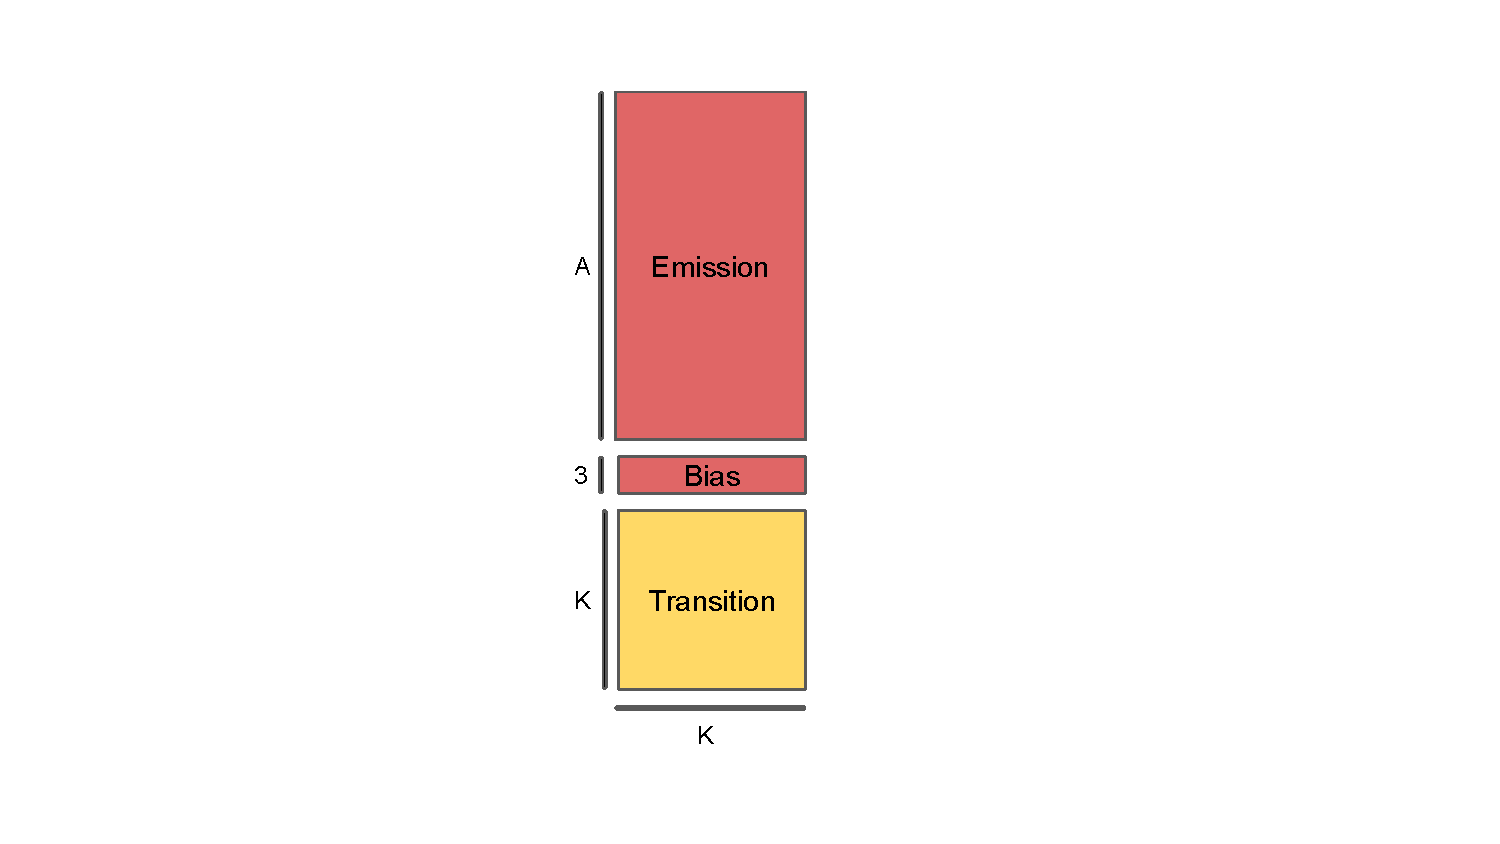
\includegraphics[width=.2\textwidth]{CRF_features.pdf}
    \caption[Sketch of sequence feature maps]{Sketch of the feature map. K is the number of different labels for one node. A is the number of attributes.}
    \label{fig:sketch feature map}
\end{wrapfigure}

The feature map has the same structure on all the data sets (cf Figure~\ref{fig:sketch feature map}).
We first draw the distinction between unary features (in red) and binary features (in yellow). The features can be written as the sum of the unary and binary features:
\begin{equation*}
	F(x, y) = \sum_{t=1}^T F_t(x_t, y_t) +  \sum_{t=1}^{T-1} F_{t, t+1}(y_t, y_{t+1}).
\end{equation*}
Unary Features depend only on the label of one node $y_t$ and the corresponding data point~$x_t$: $F_t(x_t, y_t)$.
Binary features depend only on the labels of two neighboring nodes : $F_{t, t+1}(y_t, y_{t+1})$.
It is a design choice not to directly model the relationship between two neighboring data points, e.g. $F(x_t, x_{t+1}, y_t, y_{t+1})$.
In practice the binary features simply count the number of transitions between $y_t$ and $y_{t+1}$, hence the yellow square.

For unary features, it is a bit more complex.
For each data sequence $x$, we extract an embedding for each position $t$, $\varphi(x, t)$.
For OCR, it is simply the 128 pixels image itself $\varphi(x, t) = x_t$.
For the language tasks, it is a count of the appearance of certain attributes, e.g, what is the word $x_t$, what are the words at position $t-1$, $t+1$, and so on.
A complete list of the attributes is available at \url{http://www.chokkan.org/software/crfsuite/tutorial.html}.
For each word (=node), between $13$ and $20$ features are extracted depending on the dataset.
In total the number of different attributes extracted ranges from $73,000$ to $300,000$, hence the sparsity of the features.
 We denote $A$ the number of attributes, or alternatively the size of the embedding.
 For each node with point $x_t$ and label $y_t$, $F_t(x_t, y_t)$ puts the embedding $\varphi(x, t)$ in the column indexed by $y_t$ of the red emission matrix.
 In this same column, we add some bias.
The bias part has 3 dimensions.
The first component counts the appearance of the label.
The second component counts the appearance of the label in first position of a sequence, ($t=0$).
The last component counts the number of appearance in the last position of a sequence.


\section{How to Compute the Radius of the Features}
\label{app:radius}

We drop the i index for now. We look at the pair $(x, y)$. We want to evaluate an upper bound on:
\beq
R = \|A\|^2_{1\rightarrow 2}  = \max_{y\in\cY} \| \psi(y) \|_2^2 = \max_{\tilde y\in\cY} \| F(x, y) - F(x, \tilde y)\|_2^2.
\label{app:eq:radius}
\eeq
We are using the special nature of the features to estimate this radius.
Remark that in the standard feature maps that we used (Appendix~\ref{app:feature}), there is one column per label.
If the label $y_t$ is assigned to the node $t$, then all the features extracted from that node are inserted in the column associated to $y_t$.

How to build a $\tilde y$ maximizing the distance between features?
First we build the ground truth features : $F(x, y)$.
Then we look at the labels included in the sequence $y_t$.
In each data set, the $K$ labels never appear together in one sequence.
We find a label $z$ that does not appear in the original sequence.
Then a sequence $\tilde y$ maximizing the objective~\eqref{app:eq:radius} is the sequence composed only with that label $z$.

Why? There are two reasons.
First, $F(x, y) \geq 0 \, \forall (x, y)$ thus we want $F(x, y)$ and $F(x, \tilde y)$ to have disjoint supports such that the radius can be written as:
\beq
	R = \|F(x, y) \|^2 + \|F(x,\tilde y)\|^2.
\eeq
Second, we want to maximize $\|F(x,\tilde y)\|^2$.
We need to put all the weights on few coordinates, instead of dispersing it.
This is because we look at the $\ell^2$ norm.
For the $\ell^1$ norm there would be no difference.
By repeating only one label, we effectively concentrate all the weights in one column.

Following the steps described above, we can evaluate the radii for the whole data set.


\section{A Convergence Rate on the Duality Gap}\label{app:bound duality gap}
It turns out that any algorithm with an upper bound on the primal or the dual sub-optimality for problems~\eqref{eq:primal_problem} and~\eqref{dual problem}, can get an upper bound on the duality gap for the cost of a constant.
To transpose a result of the \textit{primal} sub-optimality to the duality gap, one can go by the norm of the gradient using the smoothness of~$\cP$, that we denote $L$:
\beq
 \cP(\bw) - \cP(\bw^*)\geq \frac{1}{2L}\|\nabla \cP(\bw) \|^2 \stackrel{\eqref{eq:gradientGap}}{=} \frac{\lambda}{L} g(\bw, \hat \alpha(\bw)).
\eeq
The first inequality above is a standard one from convex analysis for convex functions with Lipschitz-continuous gradients (see e.g. \citep[eq. (2.1.6)]{nesterov_introductory_2004}).
Whatever bound we get on the primal sub-optimality, we can translate it to the duality gap by losing a constant $L/\lambda \geq \kappa$, where $\kappa$ is the condition number.

To transpose a result from the \textit{dual} sub-optimality to the duality gap, one can use the uniform ascent lemma, Equation~\eqref{app:eq:uniform ascent lemma} from Appendix~\ref{app:proof}:
\beq
	\cD(\balpha^*)  - \cD(\balpha)
	\geq \E [\cD(\balpha^+)]  - \cD(\balpha) 
	\geq \frac{s}{n} g(\hat w(\balpha), \balpha)
\eeq
where the expectation is taken over the stochasticity of the update.
Let us look at this new constant.
We know that $1/s = 1+ \frac{R}{n \lambda \strgconvex}$.
We can relate it to the smoothness $L  \approx \lambda + \frac{R}{\strgconvex}$.
This time we lose a factor $n/s \approx n + \frac{L}{\lambda} \geq n + \kappa$.
For a well-conditioned problem ($n \gg \kappa$) this is much larger than the constant we lose from the primal to the gap.


\section{Additional Comparison Plots}
\label{app:comp_plots}

We provide additional figures on the primal sub-optimality as a function of oracle calls (Figure \ref{fig:oracle_calls}), the test error as a function of epochs (Figure \ref{fig:test_err}), the  impact of reducing the precision of the Newton line-search (Figure \ref{fig:subprecision}) and the ratio between the estimate of the duality gap and the ground truth (Figure \ref{fig:ratio}).


\begin{figure}[H]
\centering
\begin{subfigure}{0.4\linewidth}
\centering
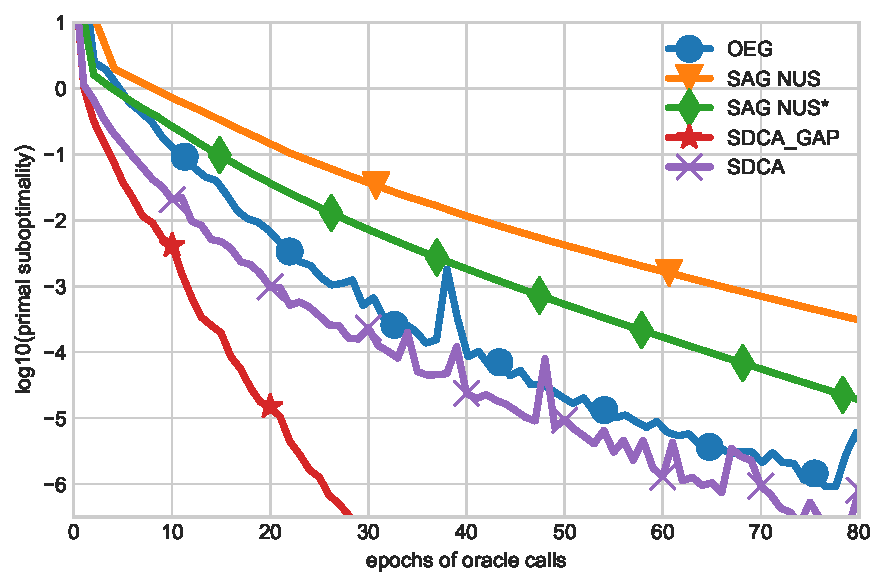
\includegraphics[width=\linewidth]{conll/primal_calls}
\caption{CONLL}
\end{subfigure}
\begin{subfigure}{0.4\linewidth}
\centering
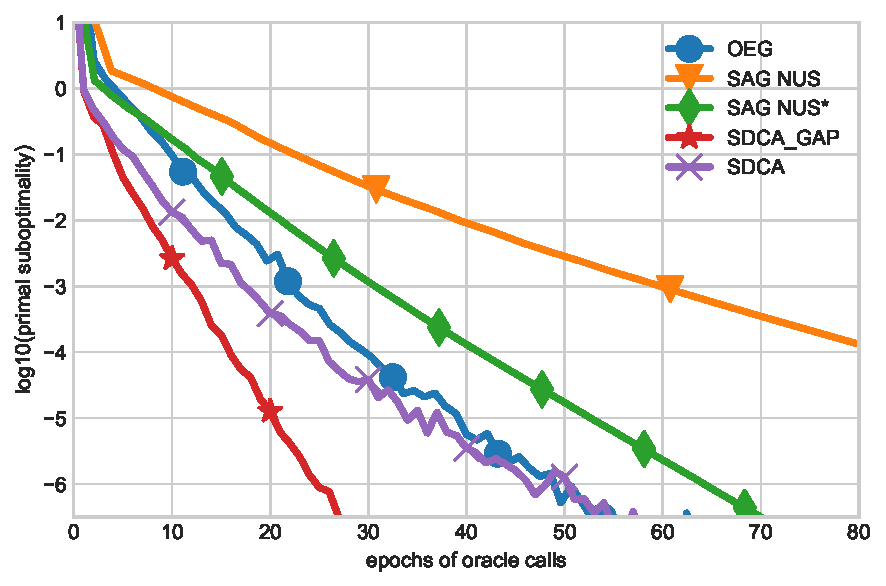
\includegraphics[width=\linewidth]{pos/primal_calls}
\caption{POS}
\end{subfigure}%
\caption[Primal sub-optimality as a function of the number of oracle calls]{Primal sub-optimality as a function of the number of oracle calls. SDCA-GAP performs much better than the competing methods for this metric partly because its line search does not require oracle calls.}\label{fig:oracle_calls}
\end{figure}

\begin{figure}[H]
\centering
\begin{subfigure}{0.4\linewidth}
\centering
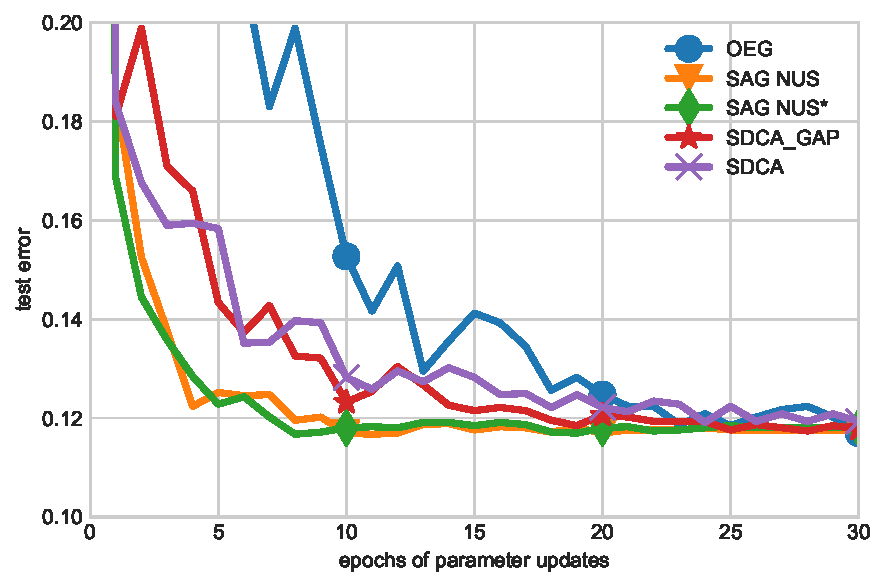
\includegraphics[width=\linewidth]{ocr/test_iter}
\caption{OCR}
\end{subfigure}%
\begin{subfigure}{0.4\linewidth}
\centering
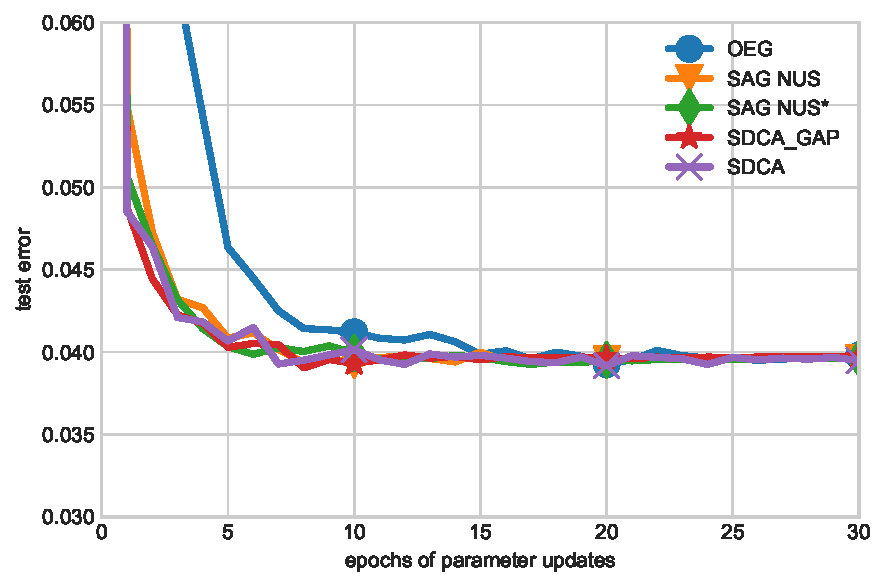
\includegraphics[width=\linewidth]{conll/test_iter}
\caption{CONLL}
\end{subfigure} \\
\begin{subfigure}{0.4\linewidth}
\centering
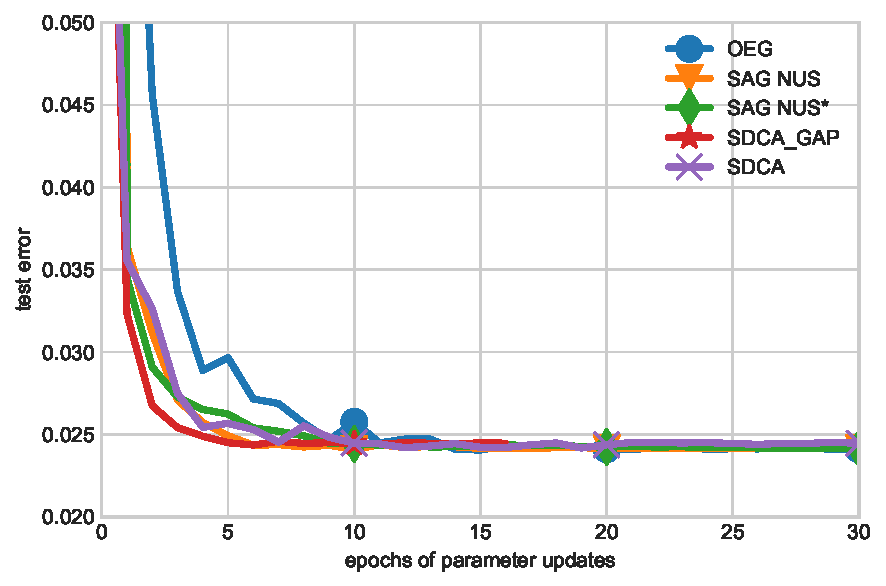
\includegraphics[width=\linewidth]{ner/test_iter}
\caption{NER}
\end{subfigure}%
\begin{subfigure}{0.4\linewidth}
\centering
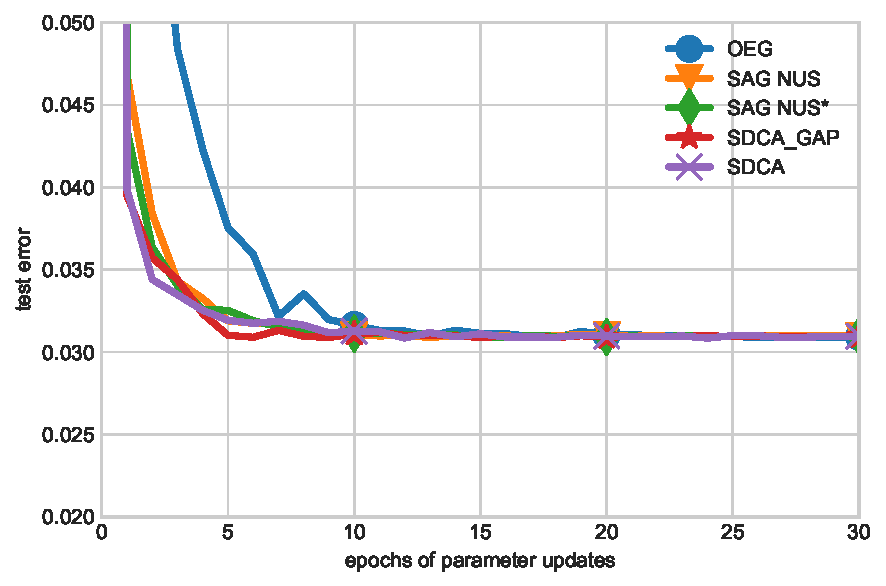
\includegraphics[width=\linewidth]{pos/test_iter}
\caption{POS}
\end{subfigure}%
\caption[Test error against number of epochs]{Test error against number of epochs. Every methods reach the same test error. SDCA and SAG have the same convergence speed.}\label{fig:test_err}

\end{figure}

\begin{figure}[H]
    \centering
    \begin{subfigure}{0.4\linewidth}
        \centering
        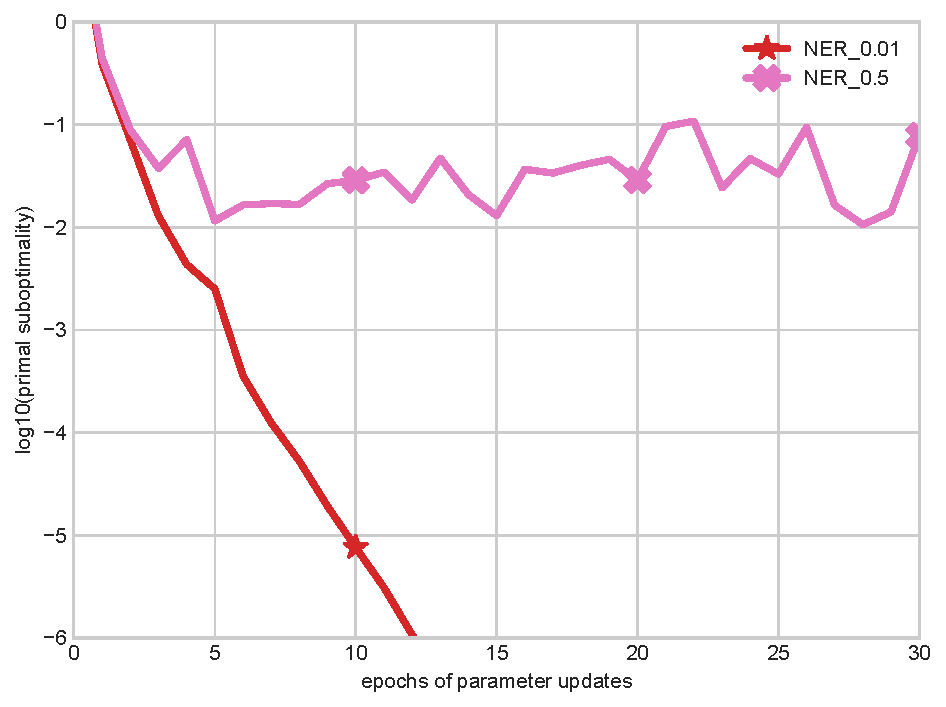
\includegraphics[width=\linewidth]{step_size_ner}
        \caption{NER}
    \end{subfigure}
    \begin{subfigure}{0.4\linewidth}
        \centering
        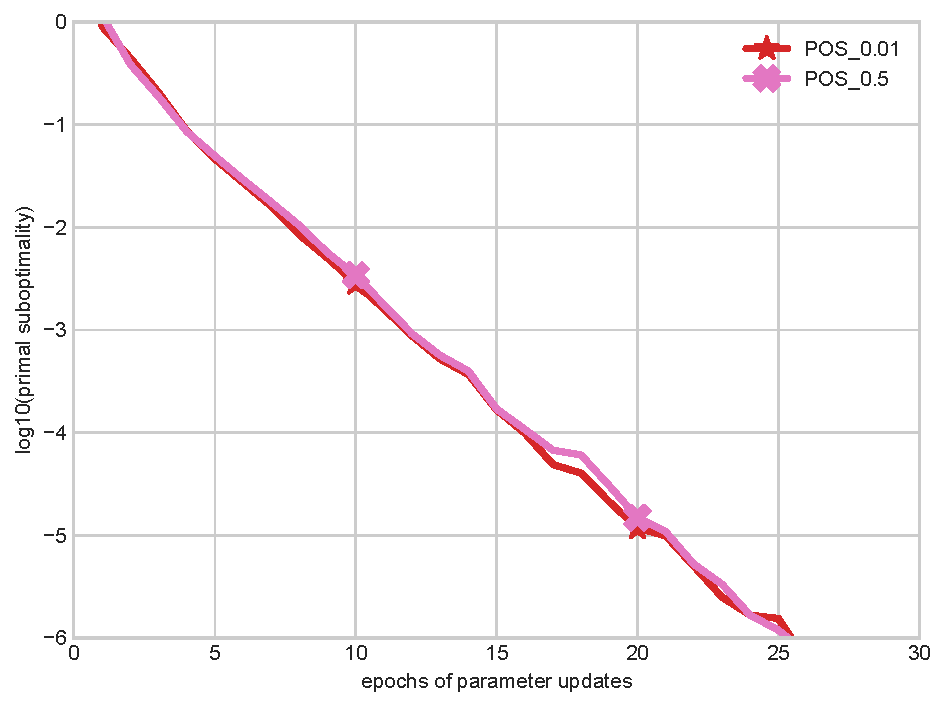
\includegraphics[width=\linewidth]{step_size_pos}
        \caption{POS}
    \end{subfigure}
	\caption[Influence of the line search precision]{
		Performance of SDCA on NER and POS with a Newton line-search.
		The number after the name of the dataset indicates the sub-precision we asked.
		A sub-precision of 0.5 effectively means that Newton stops after 1 step.
		While there is no difference between the curves for POS, 1 step of Newton update fails to converge on NER.
	}\label{fig:subprecision}
\end{figure}


\begin{figure}[H]
\centering
\begin{subfigure}{0.4\linewidth}
\centering
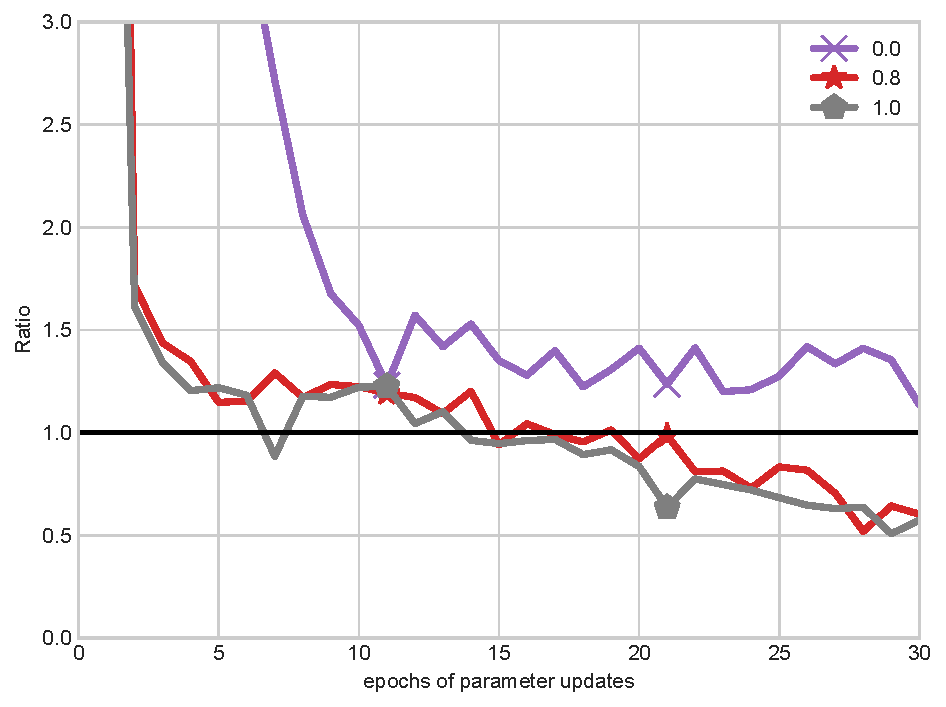
\includegraphics[width=\linewidth]{gap_ratio_conll}
\caption{CONLL}
\end{subfigure}
\begin{subfigure}{0.4\linewidth}
\centering
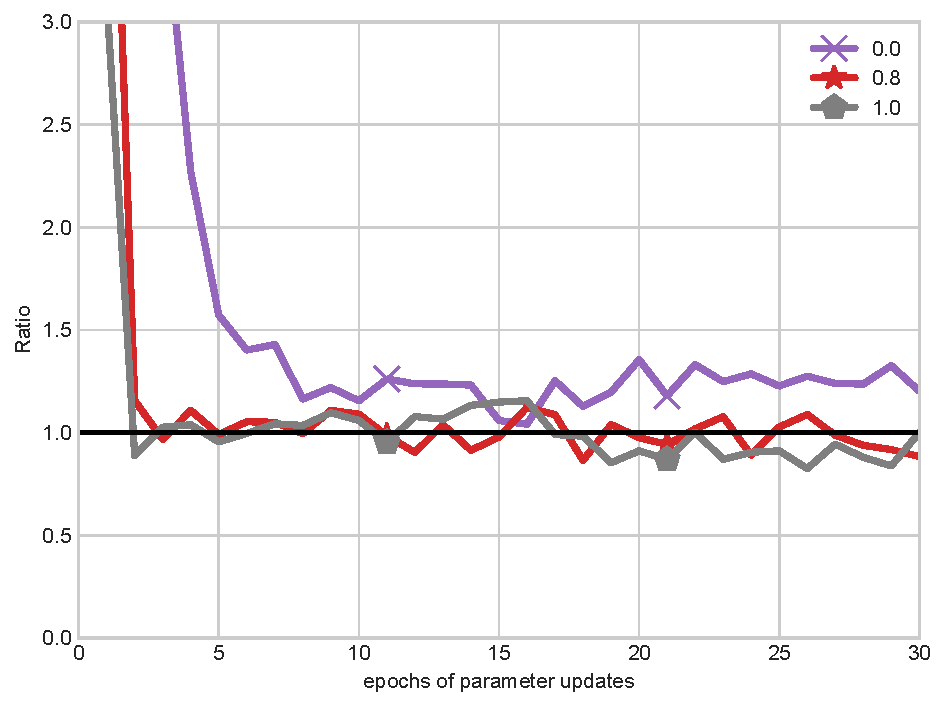
\includegraphics[width=\linewidth]{gap_ratio_ocr}
\caption{OCR}
\end{subfigure}
\caption[Duality gap estimation]{The ratio between the estimate of the duality gap and the ground truth as a function of the proportion of non uniform sampling. The gap sampling tends to underestimate this value, whereas the uniform sampling tends to over-estimate it.}\label{fig:ratio}

\end{figure}

\section{A Technical Report on Non-uniform Sampling for Stochastic Dual Coordinate Ascent}
\label{app:nusampling}

In this section, we review the proofs of convergence of SDCA and its variants with importance and residual sampling.
Then we derive bounds on the convergence rate of two new sampling scheme for SDCA.
The first scheme samples proportionally to the duality gaps of each individual variable.
The second scheme is similar to the first one, but it corrects the duality gaps with the Lipschitz constant of the primal problem.

\subsection{Setting}
We derive these bounds in a more general setting than the logistic regression, and we have to introduce some new notation.

Let $\bw$ denote the weights vector parameter, and $A_i$ the i-th features matrix.
Let $\phi$ be the primal loss function.
We suppose it is convex and $1/\strgconvex$-smooth with respect to $\|.\|_P$ (dual norm $\|.\|_D$).
The regularizer $r$ is supposed 1-strongly convex with respect to $\|.\|_{P'}$ (dual norm $\|.\|_{D'}$).
Because $\phi$ and $r^*$ are smooth, they are also differentiable. Note that every starred variable represent its dual conjugate.

The empirical loss minimization problem is:
\begin{equation}
	\label{app:primal problem}
	(P) \quad \min_{\bw \in \real^d} \lambda r(\bw) + \frac{1}{n} \sum_{i=1}^n \phi_i(-A_i^T \bw).
\end{equation}
Its Fenchel dual problem is:
\begin{equation}
	\label{app:dual problem}
	(D) \quad \max_{\balpha | \forall i, \alpha_i \in \dom \phi^*} -\lambda r^*(\hat v(\balpha)) - \frac{1}{n} \sum_{i=1}^n \phi_i^*(\alpha_i),
\end{equation}
with
\begin{equation}
	\label{app:dual to primal}
	\hat v(\balpha) := \frac{1}{\lambda n} \sum_i A_i \alpha_i \quad \textrm{and} \quad \hat w(\balpha) \in  \nabla r^* (\hat v(\balpha)).
\end{equation}
We also note:
\begin{equation}
	\label{app:primal to dual}
	\forall i, \beta_i = \hat \alpha_i(\bw) \in  \nabla \phi_i(-A_i^T \bw).
\end{equation}
Minimization of the empirical risk can often be interpreted as going around the diagram below.
\begin{displaymath}
    \xymatrix{ \bm w \ar[r] &   \nabla \phi_i(-A_i^T \bm w) \ar[d] \\
                \nabla r^* \big ( \frac{1}{\lambda n} A \balpha \big ) \ar[u] &  \balpha \ar[l] }
\end{displaymath}

We define the squared radius of the features for a given sample i as the operator norm of the matrix $A_i$:
\begin{equation}
	R_i := \|A_i\|^2_{D\rightarrow D'}.
\end{equation}
We also define the maximum squared radius as $R=\max_i R_i$ and the mean radius $\bar R = \frac{1}{n} \sum_i R_i$.

\paragraph{Log-likelihood special case.}
The loss $\phi(z)=\log(\sum_y \exp(z_y)) $ is 1-smooth with respect to the max-norm.
Its convex conjugate is the negative entropy $\phi^*(\alpha) = -H(\alpha) = \sum_y \log(\alpha_y) \alpha_y $ which is in turn 1-strongly convex with respect to the $\ell_1$-norm, and whose domain is the simplex.
We use the $\ell_2$ regularization whose dual function is itself.
We thus have $R_i =  \|A_i\|^2_{1\rightarrow 2} = \max_y \| \psi_i(y) \|_2^2$.
We also have a special expression for the primal to dual function $\beta_i = p(.|x_i; \bw) \propto \exp(-\bw^T \psi_i(.))$.
The dual variable is obtained as the conditional probability of the primal model.
Conversely, the primal weights are obtained as the expectation of the features $\psi_i(y)$, which are the columns of $A_i$.

\subsection{Duality Gaps}
We derive an interesting form on the duality gaps that support a new sampling strategy.
This is not needed to understand the convergence rates of SDCA and its variants, and the reader may skip this section.

The duality gap is:
\beq
g(\bw,\balpha) = P(\bw)-D(\balpha) = \lambda \left( r(\bw)+r^*(\frac{ A \balpha}{\lambda n}) \right) + \frac{1}{n}\sum_{i=1}^n \phi(-A_i^T\bw) +\phi^*(\alpha_i).
\eeq

Because of the two conjugate pairs $(r, r^*)$ and $(\phi, \phi^*)$ there are two apparent ways to simplify it.
One is to take the conjugate primal variable $\bw \vcentcolon= \hat w (\balpha)$, another is to take the conjugate dual variable $\balpha \vcentcolon= \hat \alpha(\bw)$.

\paragraph{Conjugate primal variable.}
Under the hypothesis $\bw = \hat w (\balpha)$, we obtain:
\beq
r(\bw)+r^*(\frac{ A \balpha}{\lambda n}) = \bw^T \frac{ A \balpha}{\lambda n}.
\eeq
The duality gap simplifies:
\beq
g(\hat w(\balpha), \balpha)
= \frac{1}{n}\sum_{i=1}^n \phi(-A_i^T \hat w(\balpha)) + \phi^*(\alpha_i) - \alpha_i^T (-A_i^T \hat w(\balpha))
= \frac{1}{n}\sum_{i=1}^n F_\phi(-A_i^T \hat w(\balpha), \alpha_i),
\eeq
where $F_\phi(s, \alpha)$ is the Fenchel duality gap~\eqref{eq:Fench} between vectors $s$ and $\alpha$.
When $\phi$ is the log-sum-exp, these vectors are the score (or logit) $s$ and the probability $\alpha$.
We want to simplify this further to directly relate $\balpha$ and its next iterate $\hat\alpha_i\circ\hat w(\balpha)$.
To do so we need another condition:
\beq
\langle \nabla \phi^* \circ \nabla \phi(s) - s , \beta - \alpha \rangle = 0,
\label{eq:condition_legendre_couple}
\eeq
for all $s\in \dom \phi$ and $\alpha, \beta \in \dom \phi^*$.
Geometrically, the pairs $(s, \nabla \phi^* \circ \nabla \phi(s) )$ should always be aligned orthogonally to $\dom \phi^*$.
This condition~\eqref{eq:condition_legendre_couple} is true whenever $\nabla \phi^* \circ \nabla \phi = \text{Id}$ the identity function.
It is also true when $\phi$ is the log-sum-exp although $\nabla \phi^* \circ \nabla \phi$ is not the identity.
Then the Fenchel duality gap is equal to the Bregman divergence generated by $\phi^*$:
\beq
F_\phi(s, \alpha) = D_{\phi^*}(\alpha || \nabla \phi (s)).
\eeq
Then the duality gap can be written as the average over data points of the $\phi^*$-Bregman divergence between $\alpha_i$ and its next fixed point iterate: $\hat\alpha_i\circ\hat w(\balpha)$:
\beq
g(\hat w(\balpha), \balpha)
= \frac{1}{n}\sum_{i=1}^n D_{\phi^*}(\alpha_i || \hat\alpha_i\circ\hat w(\balpha)).
\label{app:eq:dual_gap}
\eeq

\paragraph{Conjugate dual variable.}
The situation is quite symmetric.
Under the assumption that  $\balpha \vcentcolon= \hat \alpha(\bw)$, one gets:
\beq
g(\bw, \hat \alpha(\bw))
= \lambda \left ( r(\bw) + r^*(\frac{ A \hat \alpha(\bw)}{\lambda n})) - \bw^T\frac{ A \hat \alpha(\bw)}{\lambda n} \right )
= \lambda F_r(\bw, \frac{ A \hat \alpha(\bw)}{\lambda n}),
\eeq
where $F_r$ is the fenchel duality gap of the regularizer.
We can transform it into the Bregman divergence between $\bw$ and its next iterate $\bw' := \nabla r^*(\frac{ A \hat \alpha(\bw)}{\lambda n})) = \hat w \circ \hat \alpha(\bw)$ at the condition that:
\beq
\langle \nabla r \circ \nabla r^*(\bm v) - \bm v, \bw' -\bw \rangle = 0,
\eeq
for all vectors $\bm v$ in the domain of $r^*$ and all vectors $\bw, \bw'$ in the domain of $r$.
Then the duality gap is:
\beq
g(\bw, \hat \alpha(\bw))
= \lambda D_r(\bw ||  \hat w \circ \hat \alpha(\bw) ).
\label{app:eq:primal_gap}
\eeq

Equations~\eqref{app:eq:dual_gap} and~\eqref{app:eq:primal_gap} show that the objective~\eqref{app:primal problem} is also a fixed point problem for the conjugation operations.
The suboptimality can be easily measured as the divergence between a point, either primal or dual and its next iterate.
The divergence is given by the regularizer of the primal problem $r$ or the dual problem $\phi^*$.

%%%%%%%%%%%%%%%%%%%%%%%%%%%%%%%%%%%%%%%%%%%%%%%%%%%%
\subsection{Theorems}
\label{app:theorem}

We state the convergence rates for some variants of SDCA using non-uniform sampling. The proofs follow in the next section.

Denote $h_t := D(\balpha^*) - \E[D(\balpha^{(t)} ]$ the expectation of the dual sub-optimality at step t.
The expectation is over all the possible samplings (the stochastic part of SDCA).
We will bound this value.
One can bound the duality gap $g(\hat w(\balpha),\balpha) := P(\hat w(\balpha)) - D(\balpha)$ at the cost of another constant outside of the exponential (Appendix~\ref{app:bound duality gap}).

\begin{theorem}[Uniform sampling \citep{shalev-shwartz_accelerated_2013-1}]
	\label{app:th:uniform}
	At each step, sample $i$ with uniform probability in $[1,n]$.
	After t iterations, the dual sub-optimality is bounded by:
	\begin{equation}
		h_t \leq (1-\frac{s}{n})^t  h_0,
	\end{equation}
	where $ s = (1+ \frac{R}{n \lambda \strgconvex} )^{-1} $ is the fixed step-size used in the proof.
\end{theorem}

This theorem holds for SDCA with line search as well, since the line search can only be faster than the fixed step size.
None of the following algorithm take the line search into account.
The relative values of the bounds appearing in each theorems may not always reflect the relative
performance of each algorithms.

Intuitively, we want the linear coefficient, here $\frac{s}{n}$, to be as large as possible.
Here $R/\strgconvex$ is the max of the smoothness of the individual losses $\phi_i$.
If the regularizer is smooth enough, then the linear coefficient is related to the condition number $\kappa$ by:
\beq
\frac{n}{s}  = n + R/(\lambda \strgconvex) \approx n + \kappa.
\eeq

The following theorem goes from the maximum radius $R$ to the mean radius $\bar R$.

\begin{theorem}[Importance Sampling \citep{Zhao2015StochasticOptimizationImportance}]
	\label{app:importance}
	At each step, sample $i$ with probability $p_i$ proportional to the individual "condition number":
	\begin{equation}
		p_i \propto 1+R_i/(n \lambda \strgconvex).
	\end{equation}
	After t iterations, the dual sub-optimality is bounded by:
	\begin{equation}
		h_t \leq (1-\frac{\bar s}{n})^t  h_0,
	\end{equation}
	where $\bar s := (1 + \frac{\bar R}{n \lambda \strgconvex})^{-1}$ is the harmonic mean of the step-sizes used in the proof.
\end{theorem}

The harmonic mean is always larger than the minimum step size, so the importance sampling will converge faster than the uniform sampling \textit{at the condition} that we have an accurate estimate of the operator norms $R_i$.
Indeed, if we get the operator norms wrong, then we will sample more often points that are actually easier to classify.
Even if we estimate them right, empirical convergence may be slower with this scheme because of the line search.
This is what happened during the experiments that we ran on CRFs.

Note the similarity with non-uniform sampling in primal methods.
The convergence is improved thanks to larger step sizes, that are proportional to the inverse of some kind of Lipschitz constants.
The convergence rate depends on the arithmetic mean of these Lipschitz constants instead of the max.

We now introduce an adaptive scheme. We reformulate the theorem to make it more compact and comparable with our theorems.

\begin{theorem}[AdaSDCA \citep{csiba2015stochastic} ]
	\label{app:csiba}
	Suppose that the loss functions are \textbf{quadratic} $\phi(z):=\|z\|_2^2$.
	Denote $d_i^t =  \|\beta_i^t - \balpha_i^t \|_{D'}$
	At each step $t$, sample $i$ with probability $p_i^t$ defined by:
	\begin{equation}
		p_i^t \propto d_i^t \sqrt{1+R_i/(n \lambda \strgconvex)},
	\end{equation}

	\begin{equation}
		\theta(\bm d, \bm p) = \frac{\sum_i d_i^2}{\sum_{i | p_i >0} \frac{d_i^2}{p_i} (1+ \frac{R_i}{n \lambda \strgconvex}) },
	\end{equation}
	and
	\begin{equation}
		\tilde \theta_t =  \frac{\E[\theta(\bm d^t,\bm p^t) (P(\bw^t) - D(\balpha^t))] }{ \E[P(\bw^t) - D(\balpha^t) ] }
	\end{equation}
	where the expectation is taken over all the possible trajectories of the algorithm, e.g the sampling of the points.
	Finally define $\tilde \theta = \min_t \tilde \theta_t$.
	After t iterations, the dual sub-optimality is bounded by:
	\begin{equation}
		h_t \leq (1- \tilde \theta )^t  h_0.
	\end{equation}
\end{theorem}

In the theorem above, we have to take the expectation of some variable over all the trajectories of the algorithm.
This is not very clean, but this is unavoidable to get a general convergence result with an adaptive scheme.
Alternatively, one could simply compare the improvement given by one step for each algorithm.

A major limitation of the theorem above is that the loss has to be quadratic.
This theoretical limitation is not a big problem empirically.
It results from a symbolic trick used in the proof : setting the step-size to be proportional to the inverse of the probability.
This is reasonable for importance sampling, because the probability is proportional to the smoothness constant.
Setting the step-size to the inverse of the smoothness is optimal for gradient descent.
This may be less reasonable for other sampling schemes.

Another limitation is that we have to estimate the $n$ distances $d_i^t$ at each step.
In practice we compute $d_i^t$ only for the sampled $i$, and use the latest estimate $d_j^{t'}$ for all the other samples $j$.
Our estimates will become stale as the algorithm unfolds, but there are heuristics to compensate for that phenomenon.
One is to sample from a mixture between a uniform and an adaptive distribution.
Another is to do a batch update of the $d_i$ every once in a while.
These heuristics are unavoidable for adaptive schemes, as we do not want the cost of every update to be $O(n)$.
We do not know how  to analyze the impact of these heuristics.
Empirically, adaptive sampling with this heuristic still accelerates convergence.

Now we are going to introduce two new adaptive sampling scheme.
Both of them rely on the structure of the duality gap:
\begin{equation}
	g(\hat w(\balpha),\balpha) := P(\hat w(\balpha)) - D(\balpha) = \sum_i \phi(-A_i^T \hat w(\balpha)) + \phi^*(\alpha_i) + \langle \hat w(\balpha),  A_i \alpha_i \rangle.
\end{equation}
Each term of the sum above is a Fenchel duality gap between the loss and its convex conjugate.
They are all positive, and somehow represent the sub-optimality of the current model for every training sample.
Intuitively, sampling the most sub-optimal point may yield the best improvement.

\begin{theorem}[Gap sampling]
	\label{app:th:gap}
	At each step $t$, sample $i$ with probability $p_i^t$ proportional to the individual Fenchel duality gap:
	\begin{equation}
		p_i^t \propto g_i^t := \phi(-A_i^T \bw^t) + \phi^*(\alpha_i^t) + \langle \bw^t,  A_i \alpha_i^t \rangle.
	\end{equation}
	Define the non-uniformity of the duality gaps as the ratio between their quadratic mean and their arithmetic mean:
	\begin{equation}
	    \label{app:eq:non-uniformity}
		\chi^2(\bm g) := \frac{\frac{1}{n} \sum_i g_i^2}{  \big ( \frac{1}{n}  \sum_i g_i \big )^2 } \in [1,n].
	\end{equation}
	Take $\chi$ a lower bound on these non-uniformity over all trajectories, for all time steps.
	After t iterations, the dual sub-optimality is bounded by:
	\begin{equation}
		h_t \leq (1-s\frac{\chi^2}{n})^t  h_0.
	\end{equation}
	where $ s = (1+ \frac{R}{n \lambda \strgconvex} )^{-1} $ is the fixed step-size used in the proof.
\end{theorem}

This theorem has the same limitations relative to adaptive scheme that we mentioned for AdaSDCA.

This kind of sampling scheme was studied in the sublinear convergence regime by \citet{osokin2016minding} (Franke-Wolfe) and \citet{perekrestenko17a} (Coordinate Descent).
They could not establish a domination of gap-sampling over uniform sampling.
This is what we prove in the linear regime for SDCA since the non-uniformity $\chi$ belongs to $[1,\sqrt n]$.

The non-uniformity $\chi^2(\bm g)$~\eqref{app:eq:non-uniformity} is worth $1$ if the gaps
are all the same, and $\sqrt n$ if only one gap is non-zero, hence the name.
Gap-sampling will be $n$ times faster than uniform sampling if only one sample $i$ is suboptimal $g_i>0$.
This result is sensible since we will sample only one point, while the uniform algorithm may sample a large number first.
Let us imagine another scenario where all points are already optimal except $k$ of them which have the same gap value.
Then the acceleration coefficient will be $\frac{n}{k}$, which can be a significant acceleration when $k$ is much smaller than $n$.
Finally, consider a scenario where the gaps are evenly distributed $\{a, 2a, ..., n a\}$ for some value $a > 0$.
Note that $\chi^2(\bm g)$ is scale-invariant and does not depend on the specific value $a$.
We can compute $\chi^2(\bm g)$ explicitly here using Faulhaber's formula for the sum of powers of integers:
\begin{equation*}
\chi^2(\bm g) = \frac{\frac{1}{n} \frac{n(n+1)(2n+1)}{6}}{\left(\frac{1}{n}\frac{n(n+1)}{2}\right)^2} = \frac{2}{3} \frac{2n+1}{n+1} \approx 4/3.
\end{equation*}
The acceleration coefficient here is approximately 4/3 compared to uniform sampling.

The duality gaps are often computable, even in the Conditional Random Fields context.
On the other hand, we do not have direct access to the dual variable $\balpha$
and we cannot compute the distance $d_i = \| \beta_i - \alpha_i \|_1$, as it is the $\ell^1$ norm of a vector of exponential size.

Now we want to combine importance sampling with duality gap sampling.
We would like to benefit both from the dependency on $\bar R$ and the acceleration by $\chi$.

\begin{theorem}[Lipschitz-gap sampling]
	\label{app:th:gap+}
	At each step $t$, sample $i$ with probability $p_i^t$ defined by:
	\begin{equation}
		p_i^t \propto g_i^t (1+ R_i/(n \lambda \strgconvex)).
	\end{equation}
	Define $\chi$ as in~\eqref{app:eq:non-uniformity} from Theorem \ref{app:th:gap}.
	Define $\tilde s$ as the quadratic harmonic mean of the step-sizes $s_i := 1/(1+ R_i/(n \lambda \strgconvex))$.
	After t iterations, the dual sub-optimality is bounded by:
	\begin{equation}
		h_t \leq (1-\tilde s \frac{\chi}{n})^t  h_0.
	\end{equation}
\end{theorem}

This theorem makes apparent a trade-off between the advantage gained with the smoothness,
and the advantage gained with the individual gaps.
We lose the square factor on the non-uniformity compared to Theorem \ref{app:th:gap}.
We go from the harmonic mean to the quadratic harmonic mean (generalized norm $-2$) of the step sizes,
which is basically the same as going from the arithmetic mean of the smoothness to the quadratic mean of the smoothness.
Recall that the quadratic mean always lies in between the arithmetic mean and the max.

Our results holds for any smooth loss function, contrary to AdaSDCA.
Our two new strategies complement importance sampling as none of them dominates the other.
Which one is the best depends on the context.
\textit{That is} at the condition that we have access to the $R_i$.
Otherwise gap sampling remains available.

%%%%%%%%%%%%%%%%%%%%%%%%%%%%%%%%%%%%%%%%%%%
\subsection{Proofs}
\label{app:proof}

\begin{lemma}[General descent lemma]
\label{app:th:ascent_lemma}
    Apply the SDCA update on the dual variable $\balpha$ to get the new point $\balpha^+$.
    The block $i$ is sampled with probability $p_i$ and updated with a step size $s_i$.
    The expected dual improvement verifies the lower bound:
	\begin{equation}
		n \mathbb E_{\bm p}[D(\balpha^+)] - D(\balpha)
		\geq \underbrace{ \sum_i p_i s_i g_i }_{ \textrm{not the duality gap}}
		+ \frac{\strgconvex}{2} \sum_i p_i s_i
		\bigg ( 1 - s_i  \underbrace{\left (1 + \frac{R_i}{\strgconvex \lambda n} \right )}_{:=c_i} \bigg ) d_i^2
	\end{equation}
    where $\mathbb E_{\bm p}$ denotes the conditional expectation over the choice $i \sim \bm p$
    of block to update, conditioned on the previous state $\balpha$.
\end{lemma}

\begin{proof}[Proof of Lemma \ref{app:th:ascent_lemma}]
This statement is similar to a weighted combination of Equation~(25) from~\citet{shalev-shwartz_accelerated_2013-1}. We provide here the derivation to be self-contained.
    Suppose we sampled the point $i$ and updated the block $\alpha_i$ with step size $s_i$:
    \begin{equation}
        \alpha_i^+ := \alpha_i + s_i \delta_i =  (1- s_i)\alpha_i + s_i \beta_i \, .
    \end{equation}
    The dual improvement is:
    \begin{equation}
    \label{app:eq:dual_improvement}
        n (D(\balpha^+) - D(\balpha))
        = \underbrace{ \lambda n \left( r^* \left (\frac{A \balpha}{\lambda n} \right) - r^* \left( \frac{A \balpha^+}{\lambda n} \right)  \right ) }
        _{\text{data fidelity}}
        + \underbrace{\phi^*(\alpha_i) - \phi^*(\alpha_i^+)}
        _{\text{regularization}} \, .
    \end{equation}

    We first bound the data fidelity term.
    We use the the fact that $r^*$ is 1-smooth with respect to $\|.\|_{D'}$ to upper-bound its variation:
\alignn{
        r^* \left( \frac{A \balpha^+}{\lambda n} \right)
        &= r^* \left( \frac{A \balpha}{\lambda n} + s_i \frac{A_i \delta_i}{\lambda n} \right) \\
        &\leq r^* \left( \frac{A \balpha}{\lambda n} \right)
        + s_i \left \langle \nabla  r^* \left( \frac{A \balpha}{\lambda n} \right), \frac{A_i \delta_i}{\lambda n} \right \rangle
        + \frac{s_i^2}{2} \norm{ \frac{A_i \delta_i}{\lambda n} }_{D'}^2
}
    The linear coeficient of this lower boudn is $\hat w( \balpha) = \nabla  r^* \left( \frac{A \balpha}{\lambda n} \right)$.
    The quadratic term can be further upper-bounded:
    \begin{equation}
        \norm{ \frac{A_i \delta_i}{\lambda n} }_{D'}^2
        \leq \frac{1}{(\lambda n )^2} \norm{A_i}_{D \rightarrow D'}^2 \norm{\delta_i}_{D}^2
        = \frac{R_i d_i^2}{(\lambda n )^2} \, ,
    \end{equation}
    by definition of the radius $R_i$ and the residue $d_i := \norm{\beta_i - \alpha_i}_D$.
    So the loss variation is lower bounded by:
    \begin{equation}
    \label{app:eq:bound_loss}
        \lambda n \left( r^* \left (\frac{A \balpha}{\lambda n} \right) - r^* \left( \frac{A \balpha^+}{\lambda n} \right)  \right )
        \geq s_i \left \langle \hat w( \balpha) , A_i (\alpha_i - \beta_i) \right \rangle
        - \frac{s_i^2}{2} \frac{R_i d_i^2}{\lambda n } \, .
    \end{equation}

    Now we bound the regularization term.
    Since $\phi^*$ is $\strgconvex$-strongly convex with respect to $\|.\|_D$,
    \begin{equation}
        \phi^*(\alpha_i^+)
        = \phi^*((1- s_i)\alpha_i + s_i \beta_i )
        \leq (1- s_i) \phi^*(\alpha_i) + s_i \phi^*(\beta_i)
        - s_i (1 - s_i ) \frac{\strgconvex}{2} d_i^2 \, .
    \end{equation}
    The regularization variation can be lower bounded by:
    \begin{equation}
    \label{app:eq:bound_regularization}
        \phi^*(\alpha_i) - \phi^*(\alpha_i^+)
        \geq s_i \left ( \phi^*(\alpha_i) -  \phi^*(\beta_i) \right )
        + s_i (1 - s_i ) \frac{\strgconvex}{2} d_i^2 \, .
    \end{equation}

    Plugging the bounds~\eqref{app:eq:bound_loss} and~\eqref{app:eq:bound_regularization} into Equation~\eqref{app:eq:dual_improvement}, we get:
\alignn{
        & n (D(\balpha^+) - D(\balpha)) \notag \\
        & \geq s_i \left (\phi^*(\alpha_i)
        + \left \langle \hat w( \balpha) , A_i (\alpha_i - \beta_i) \right \rangle
         -  \phi^*(\beta_i) \right )
         + \frac{s_i}{2} \left ( (1 - s_i ) \strgconvex - s_i \frac{R_i}{\lambda n } \right ) d_i^2 \, .
}
    Recall that $\beta_i := \nabla \phi (-A_i^T \hat w (\balpha))$. Thus,
    \begin{equation}
        \left \langle - A_i^T \hat w( \balpha) , \beta_i \right \rangle - \phi^*(\beta_i)
        = \phi(- A_i^T \hat w( \balpha))
    \end{equation}
    by definition of the convex conjugate $\phi^*$.
    To sum up, at iteration t, if we sample the block i, and update it with step size $s_i$,
    we can lower bound the resulting dual improvement with:
\alignn{
        \label{app:one point descent}
        & n (D(\balpha^+) - D(\balpha)) \notag \\
        & \geq s_i \underbrace{ \big [ \phi(-A_i^T \hat w(\balpha)) + \phi^*(\alpha_i) + \hat w(\balpha)^T A_i \alpha_i \big ]
        }_{ \textrm{Fenchel gap} =: g_i}
        + \frac{s_i \strgconvex}{2} \left ( 1 - s_i\left (1 + \frac{R_i}{\strgconvex \lambda n } \right )  \right )  d_i^2 \, .
 }
    To conclude the proof, take a weighted average of the inequalities~\eqref{app:one point descent} with the weights $p_i$.
\end{proof}

In the following we note the duality gap:
\begin{equation}
    \bar g := \frac{1}{n} \sum_i g_i = P(\hat w(\balpha)) - D(\balpha) \, .
\end{equation}

%%%%%%%%%%%%%%%%%%%%%%%%%%%%%%%%%%%%%%%%%%%%%%%%%%%%%%%%%%%%%%%%%%%%%%%%%%%%%%%%%%%%%%%%%%%%%%%%%%
\begin{proof}[Proof of Theorem \ref{app:th:uniform}]
    In the original proof of \citet{shalev-shwartz_accelerated_2013-1}, we set $p_i=1/n$ and $s_i = s = (1+ \frac{R}{n \lambda \strgconvex} )^{-1}  \leq 1/c_i$. This step size guarantees that the right hand term is positive, leaving us with the inequality:
    \begin{equation}
        \mathbb E_{p^t}[D(\balpha^{t+1}) - D(\balpha^t)]
        \geq \frac{s}{n} \bar g^t.
        \label{app:eq:uniform ascent lemma}
    \end{equation}
    Now observe that $\mathbb E_p[D(\balpha^+) - D(\balpha)] = - \mathbb E_p[h_{t+1}] + h_t$ and $\bar g^t = (P(\bw^t) - D(\balpha^t)) \geq h_t$.
    Moving the sub-optimality at time $t$ on the right gives:
    \beq
        \mathbb E_p[h_{t+1}] \leq (1- \frac{s}{n} ) h_t.
    \eeq
    This inequality is conditional on all the random sampling until time $t$.
    Let us take the expectation of this inequality with respect to all this past randomness.
    We get a recursive upper bound on the expected dual sub-optimality:
    \beq
        \mathbb E [h_{t+1}] \leq (1- \frac{s}{n} ) \mathbb E [h_t] \leq (1- \frac{s}{n} )^t h_0.
    \eeq
    This is the final convergence result with the linear constant $s/n = (n+R/(\lambda \strgconvex))^{-1}$.
\end{proof}

In the proof above, we lower bound the dual improvement by the duality gap, then we use this to get the linear convergence rate.
All the proofs follow the same reasoning, and the last few steps are always the same so we will skip them.

\begin{proof}[Proof of Theorem \ref{app:importance}]
    Inject $p_i=c_i/\sum_j c_j$ and $s_i = 1/c_i$. The right hand term is zero thanks to the step-size, hence the lower bound:
    \begin{equation}
        \mathbb E_p[D(\balpha^+) - D(\balpha)]
        \geq \frac{\bar g}{\sum_i c_i} .
    \end{equation}
    We get the linear rate   $\frac{1}{\sum_i c_i}$ which is also the harmonic mean of the step-sizes divided by $n$.
\end{proof}

\begin{proof}[Sketch of Proof of Theorem \ref{app:csiba}]
To make the duality gap appear in this formula for arbitrary probability $p$, \citet{csiba2015stochastic} use $p_i s_i = \theta$ constant, whenever $g_i > 0$.
If the individual duality gap is null $g_i=0$, then they set $p_i=s_i=0$.
\begin{equation}
    \mathbb E_p[D(\balpha^+) - D(\balpha)] - \theta \bar g
    \geq \theta \frac{\strgconvex}{2 n} \sum_i  d_i^2\bigg ( 1 -  \frac{\theta}{p_i} \big ( 1 - \frac{R_i^2}{\strgconvex \lambda n} \big ) \bigg )
\end{equation}

The negative consequence of that strategy is that they have to enforce $s_i \in [0,1]$ by setting
$\theta < \min_i p_i$ where the minimum is taken over the sub-optimal i's (i.e. $p_i>0$).
This a terrible constraint on the step size, as we cannot be too non-uniform without taking very small steps.
It effectively reduces the linear convergence constant $\theta /n$.

Finally, they want to maximize $\theta$ while keeping the right hand side positive.
This is a hard problem on $\theta$ and $p$.
When the loss is the quadratic loss, they can remove the condition that the step-size should be smaller than 1.
Then they solve the optimization problem to get the sampling scheme $p_i \propto d_i \sqrt c_i$.
\end{proof}

\begin{proof}[Proof of Theorem \ref{app:th:gap}]
    We use the same step-size as in the original proof:
    \begin{equation}
        s_i = s = \frac{n}{n+R/(\lambda \strgconvex)}.
    \end{equation}
    We have the guarantee that the right hand term is positive. The lemma simplifies to:
    \begin{equation}
        n \mathbb E_p[D(\balpha^+) - D(\balpha)]
        \geq \frac{s}{n} \sum_i p_i g_i.
    \end{equation}
    We inject $p_i= \frac{g_i}{n\bar g}$ into this lower bound:
    \begin{equation}
        \mathbb E_p[D(\balpha^+) - D(\balpha)]
        \geq \frac{s}{n} \frac{\sum_i g_i^2}{\sum_j g_j}
        = \frac{s}{n} \chi^2(\bm g) \bar g\, ,
    \end{equation}
    where we introduced the non-uniformity of the duality gaps vector defined in Equation~\eqref{app:eq:non-uniformity}.
    To get a simpler expression for a global convergence bound, let us define $\chi$ to be a lower bound on $\chi(\bm g)$ over all the possible unfolding of SDCA and for every steps.
    Now we can write the descent lemma in the same form as in the original proof, but a with new constant:
    \begin{equation}
        \mathbb E_p[D(\balpha^+) - D(\balpha)]
        \geq \frac{s}{n} \chi^2 \bar g\, .
    \end{equation}
\end{proof}

\begin{proof}[Proof of Theorem \ref{app:th:gap+}]
	We set $p_i \propto g_i c_i$ where $c_i = 1+ R/(n \lambda \strgconvex)$.
	\begin{equation}
		n \mathbb E_p[D(\balpha^+) - D(\balpha)]
		\geq \frac{ \sum_i s_i g_i^2 c_i}{\sum_i g_i c_i}
		+ \frac{ \frac{\strgconvex}{2}  \sum_i s_i  g_i c_i d_i^2 \
		\big ( 1 - s_i c_i \big) }{\sum_i g_i c_i}
	\end{equation}
	Similarly to the proof of importance sampling, we now set $s_i= 1/c_i \leq 1$ instead of $s_i=s=1/\max_i c_i$.
	This nullifies the right hand term.
	We can take longer steps if the individual Lipschitz constants are high.
	\begin{equation}
		n \mathbb E_p[D(\balpha^+) - D(\balpha)]
		\geq \frac{ \sum_i g_i^2 }{\sum_i g_i c_i} = \frac{\langle \bm g, \bm g \rangle}{\langle \bm c, \bm g \rangle}
	\end{equation}
	We apply the Cauchy-Schwartz inequality : $\langle \bm c, \bm g \rangle \leq \|\bm c\|_2 \|\bm g \|_2$.
	 \begin{equation}
		n \mathbb E_p[D(\balpha^+) - D(\balpha)]
		\geq \frac{ \|g\|_2 }{\|c\|_2}
		=  \frac{\chi(g)}{\QM(c)} \bar g \, ,
	\end{equation}
	where $\QM$ denotes the quadratic mean. Finally we divide both sides by n to complete the proof:
	\begin{equation}
		\mathbb E_p[D(\balpha^+) - D(\balpha)]
		\geq \frac{ \chi(g) }{n \QM(c)} \bar g \, .
	\end{equation}
\end{proof}

\end{subappendices}

\setcounter{corA}{0} % Pour recommancer à compter les defs, theorems, etc. à partir de 1
\setcounter{theorem}{0}
%\setcounter{definition}{0}
%\setcounter{proposition}{0}
%\setcounter{lemma}{0}


 % some custom math commands
\newcommand*{\entropy}{\mathcal{H}}
\newcommand*{\softargmax}{p \circ}

\newcommand*{\ptrue}{\ensuremath{\bm{p}}}
\newcommand*{\causalvar}{\theta_\rightarrow}
\newcommand*{\antivar}{\theta_\leftarrow}
\newcommand*{\pmodel}{\ensuremath{\bm{p}_{\causalvar}}}
\newcommand*{\panti}{\ensuremath{\bm{p}_{\antivar}}}

\newcommand*{\ptransfer}{\ptrue^*} 
\newcommand*{\natgauss}{\cN_\text{nat}}
\newcommand*{\chogauss}{\cN_\text{cho}}
\newcommand*{\Dir}{\mathrm{Dir}}
\newcommand*{\uniform}{\vu}
\newcommand*{\lr}{\gamma}

\newcommand{\mm}{m}
\newcommand{\logpartition}{A}
\newcommand{\alpin}{\alpha}
\newcommand{\nn}{n}
\newcommand{\logpartitionb}{B}
\newcommand{\betin}{\beta}
\newcommand{\red}[1]{{\color{red}#1}}

\newcommand*{\smoothness}{B}
\newcommand*{\strongconvexity}{\mu}
\newcommand*{\gradientvariance}{\sigma^2}


%\part{Second Contribution}

\chapter{Prologue to the Second Contribution}

\section{Article Details}

\textbf{An Analysis of the Adaptation Speed of Causal Models.} 
\emph{R\'emi Le Priol, Reza Babanezhad Harikandeh, Yoshua Bengio, Simon Lacoste-Julien.} 
This paper was published at AISTATS 2021~\citep{lepriol2021analysis}.

\section{Contributions of the authors}
Rémi Le Priol derived the comparison between distances for all models, wrote the code, ran the experiments and contributed to the general writing of the paper.
Reza Babenezhad contributed to the general writing and found the optimization method and the convergence rate for normal variables.
Simon Lacoste-Julien came up with the idea of using convergence rates to quantify the adaptation speed, while Yoshua Bengio came up with the idea of measuring the adaptation speed in the first place. 
Simon Lacoste-Julien and Yoshua Bengio supervised this project. 

\chapter{An Analysis of the Adaptation Speed of Causal Models}

\section*{Abstract}
Consider a collection of datasets generated by unknown interventions on an unknown structural causal model $G$.
Recently, \citet{bengio2019meta} conjectured that among all candidate models, $G$ is the \emph{fastest to adapt} from one dataset to another, along with promising experiments. 
Indeed, intuitively $G$ has less mechanisms to adapt, but this justification is incomplete.
Our contribution is a more thorough analysis of this hypothesis.
We investigate the adaptation speed of cause-effect SCMs.
Using convergence rates from stochastic optimization, we justify that a relevant proxy for adaptation speed is distance in parameter space after intervention.
Applying this proxy to categorical and normal cause-effect models, we show two results.
When the intervention is on the cause variable, the SCM with the correct causal direction is advantaged by a large factor.
When the intervention is on the effect variable, we characterize the relative adaptation speed. 
Surprisingly, we find situations where the anticausal model is advantaged, falsifying the initial hypothesis.
Source code for all experiments is hosted at 
\url{https://github.com/remilepriol/causal-adaptation-speed}.


\section{Introduction}

A learning agent interacting with its environment should be able to answer questions such as ``what will happen to $Y$ if I change $X$''.
Structural Causal Models (SCM) offer a formalism to answer this kind of questions \citep{pearl2009causality,peters2017elements}. 
The simplest SCM is the model $X\rightarrow Y$ where $X$ is the cause and $Y$ the effect.
Modifying $X$ will modify $Y$ but modifying $Y$ will not alter $X$.
In general, SCMs model the distribution of observations with a directed graph where edges represent \textit{independent mechanisms} \citep{janzing2010causal}.

\begin{wrapfigure}[6]{l}{.5\textwidth} 
    \centering
    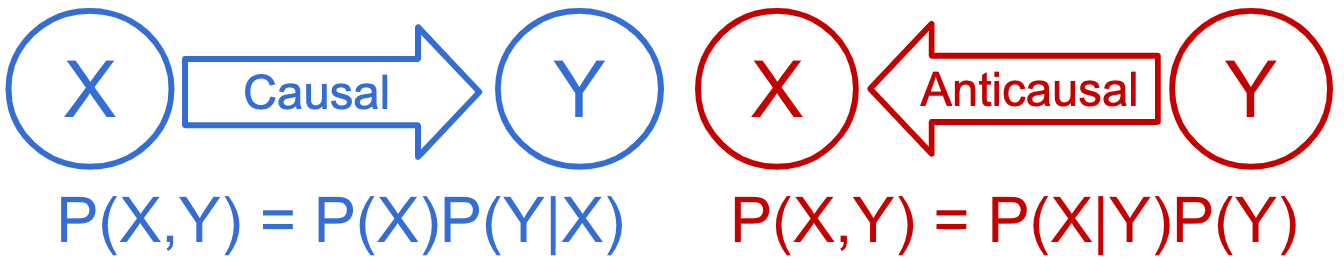
\includegraphics[width=.48\textwidth]{models.png}
    \caption{Two models for data $(X, Y)$ with causal structure $X\rightarrow Y$.}
    \label{fig:cause-effect}
\end{wrapfigure}

Modern machine learning methods can fail surprisingly when the test distribution differ from the training distribution \citep{rosenfeld2018elephant}. 
A recent line of work describes these distribution shifts as interventions in an underlying causal model \citep{zhang2013domain, magliacane2018domain}. 
If this description is accurate, then an agent endowed with this hypothetical causal model could handle distribution shifts by updating the few mechanisms affected by the intervention.
On contrary, an agent endowed with an incorrect model, would have to update many mechanisms.
\citet{bengio2019meta} infer that the causal agent will be the fastest to adapt to distribution shifts.
Conversely, they use the speed of adaptation to unknown interventions as a criterion to learn the true causal model, showing promising empirical results on cause-effect models.
Yet they lack a theoretical argument to connect interventions and fast adaptation. Thus we raise the question: 

\textit{Do causal models adapt faster than non-causal models to distribution shifts induced by interventions?}

\paragraph{Contributions.}
We theoretically and empirically answer this question for cause-effect SCMs with categorical variables, and partially  for multivariate normal distributions. 
\begin{itemize}
    \item For both settings, we use stochastic optimization convergence rates to show that the adaptation speed mostly depends on the distance in parameter space between the initialization (before intervention) and the optimum (after intervention).
    \item For categorical variables, we fully characterize this distance. We show that the causal model is faster by a large factor when the intervention is on the cause. 
    \item When the intervention is on the effect, we surprisingly find settings where the anticausal model is systematically faster. As appealing as the fastest-to-adapt hypothesis may sound, it does not hold in every situations.
\end{itemize}


\begin{figure*}
    \centering
    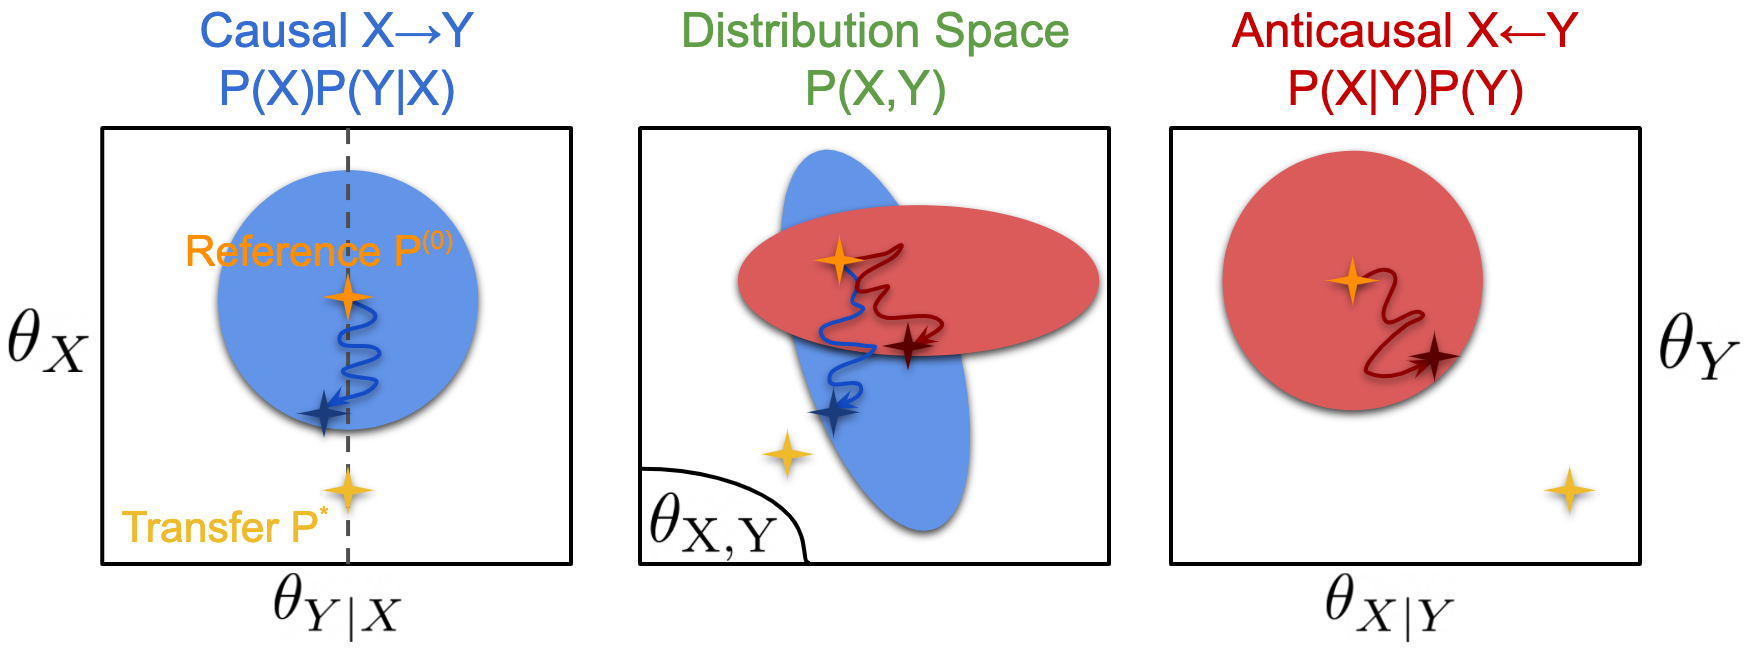
\includegraphics[width=\textwidth]{geometry.png}
    \caption[Intuition behind fast adaptation]{
    \textbf{Intuition behind fast adaptation.}
    An intervention on $X$ turns the reference distribution $\ptrue^{(0)}$ into  a transfer distribution $\ptrue^*$.
    The causal model (blue) only has to adapt $\theta_X$, whereas the anticausal  model (red) has to adapt both its mechanisms. 
    After adaptation, the causal model ends up the closest from the transfer in terms of KL, as visible in the abstract distribution space. 
    Blue and red balls represent
    the \textit{proximity prior} induced by taking a few steps of SGD from the reference in each parameter space.
    Convergence rate analysis reveals that they are spherical functions of the parameter distance,
    but they get mapped to non-trivial shapes in distribution space -- ellipses in this sketch.
    }
    \label{fig:geometry}
\end{figure*}

\section{Related work}

Causal relationships are asymmetric.
These asymmetries are often visible in observations, so that one can identify which is cause and which is effect under relevant assumptions \citep{mooij2016distinguishing}. 
A common assumption is to constrain the set of functional dependencies between cause and effect. 
By contrast, in our work, we focus on two families of distributions which are notoriously unidentifiable from observational data: categorical and linear normal variables \citep[Ch.4]{peters2017elements}.
With data coming from a generic directed acyclic graph (DAG), we can only hope to discover the Markov equivalence class of this DAG \citep{verma1991equivalence}.
Many methods seek to achieve this goal, whether constraint-based such as the PC algorithm \citep{spirtes2000causation} or score-based methods using greedy search \citep{chickering2002optimal} or more recently continuous optimization \citep{zheng2018dags,lachapelle2019gradient}.
However to discover the exact graph, we need access to interventional data.

Inferring  causal links from interventions or experiments is the foundation of science. 
Inferring causal links from unknown interventions is a much harder and less principled problem.
\citet{tian2001causal} first studied this setting, proposing a constraint based method to infer the interventional equivalence class  from a sequence of interventions.
Then \citet{eaton2007exact} proposed an exact Bayesian approach.
More recently, \citet{squires2019permutation,ke2019learning}  proposed score based algorithms, improving in scalability and alleviating parametric assumptions.
From a machine learning perspective, we are concerned with the predictive power that this structure will give us when faced with new data.




Distribution shifts are a common problem in machine learning, as well as in causal statistics \citep{zhang2013domain, pearl2014external}.
\citet{scholkopf2012causal} first brought up the idea of \emph{invariance} to tackle this problem.
Following up on this idea, \citet{peters2016causal} designed an algorithm able to identify robust causal features from heterogeneous data.
This work has set a fruitful line of research for robust machine learning \citep{heinze2018invariant, heinze2018causal, rothenhausler2019causal, arjovsky2019invariant}.
In a way, fast adaptation is the complementary idea of invariance: if most mechanisms are kept invariant, then only a few have to adapt. 
\citet{scholkopf2019causality} shed light on these approaches and the broader scope of causality research for machine learning.

\section{{Background}}

In this section, we review the formalism of \citet{bengio2019meta} on observations, interventions, models and adaptation.

\paragraph{Reference and Transfer Distributions.}
We assume perfect knowledge of a reference distribution $\ptrue$ over the pair $(X,Y)$ sampled from an SCM $X\rightarrow Y$. This distribution is the object of interventions, which results in new \emph{transfer} distributions $\ptransfer$.
If the \textit{intervention is on the cause}, $X$ is sampled from a different marginal, then $Y$ is sampled from the reference conditional
\begin{equation}
    \ptransfer(x,y) = \ptransfer(x) \ptrue(y|x) \; .
\end{equation}
If the \textit{intervention is on the effect}, $X$ is sampled from the reference marginal, then $Y$ is sampled from another marginal independently of $X$
\begin{equation}
    \ptransfer(x,y) = \ptrue(x) \ptransfer(y) \; .
\end{equation}
For each transfer distribution, we observe a few samples. 


\paragraph{Models.} 
We parametrize two generative models of~$(X, Y)$ (Fig.~\ref{fig:cause-effect}):
\begin{align}
    \pmodel (x, y) = \ptrue_{\theta_X}(x)  \ptrue_{\theta_{Y|X}}(y|x)  \quad 
    &\textit{-- causal} \label{eq:causal_eq}\\
    \panti (x,y) = \ptrue_{\theta_Y}(y)  \ptrue_{\theta_{X|Y}}(x|y) \quad 
    &\textit{-- anticausal}  \label{eq:anti_causal_eq}\; .
\end{align}
For each model, we call mechanisms the marginal and conditional models.
Each mechanisms has its own set of parameters, e.g. $\theta_X$ and $\theta_{Y|X}$.
In the following we will use $\theta$ to denote interchangeably $\causalvar$ and $\antivar$.

\paragraph{Adaptation.}
Both models are initialized to fit perfectly the reference distribution $\ptrue_{\causalvar^{(0)}} = \ptrue_{\antivar^{(0)}} = \ptrue$.
They observe fresh samples from $\ptransfer$ one by one and update their parameters $\causalvar$ and $\antivar$  to maximize the log-likelihood with a step of stochastic gradient (SGD).
Thanks to the separate parameters, the causal model log-likelihood loss decomposes as
\begin{align}
    &  \cL_\text{causal}(\causalvar)
    = \expect[(X,Y) \sim \ptransfer]{-\log \pmodel(X,Y)}\nonumber
    \\ = & \expect[\ptransfer]{-\log \ptrue_{\theta_X}(X)} + \expect[\ptransfer]{-\log \ptrue_{\theta_{Y|X}}(Y|X)}
    \label{eq:causal_loss}
\end{align}
When $\ptransfer$ comes from an intervention, \citet{bengio2019meta} observe that the causal model is often faster to adapt than the anticausal model.
Intuitively, this is because the causal model has to adapt only the mechanism which was modified by the intervention.
On the other hand, the anticausal model has to adapt both its mechanisms. In Figure~\ref{fig:geometry}, we compare these different scenarios and the concept of adaptation figuratively.
While appealing, \emph{this reasoning is not rigorous}, as sample complexity bounds of SGD typically do not depend on the number of parameters to update \citep[Th. 6.2 \& 6.3]{bubeck2015convex}.
In the next section, we formalize and understand this phenomenon in the light of convergence rates of stochastic optimization methods.

\paragraph{Distribution Families.} 
We study two of the simplest sub-families of the exponential family \citep{wainwright2008graphical}: categorical and linear normal variables.
Their negative log-likelihood is a convex function of their natural parameter.
These families are interesting because the direction is not identifiable from observational data  \citep[Ch.4]{peters2017elements}
-- e.g. $\pmodel$ and $\panti$ can model the same set of distributions -- 
which makes them challenging for causal discovery.

\section{An optimization perspective}
\label{sec:opt_alg}
One way to formalize adaptation speed is to characterize it via the convergence speed of the stochastic optimization procedure. An appealing aspect of stochastic optimization algorithms such as SGD (when only using fresh samples and running it on the true loss we care about) is that they come with convergence rate guarantees on the \emph{population risk} in machine learning, thus giving us direct sample complexity results to obtain a specific generalization error.
The convergence rate is an \emph{upper bound} on the expected suboptimality after a given number of iterations.
While these rates are about worst case performance and might also be loose, fortunately, for convex optimization, they tend to correspond well to actual empirical performance~\citep{nesterov2004Intro}.
We can thus use the convergence bounds as theoretical proxy for the convergence speed.
In our experiments, we also verify empirically that the bounds correlate well with the observed convergence speed.

Here we provide a classical convergence rate on the expected suboptimality with Average Stochastic Gradient Descent (ASGD) under convexity and bounded gradient assumptions. 
We re-derive this rate in Appendix~\ref{apdx:asgd_rate} for completeness.
This rate applies to log-likelihood maximization for categorical random variables (details in~\ref{apdx:categorical_optimization}). 
Since the target distribution is part of the model family, the log-likelihood suboptimality is equal to the KL-divergence  -- e.g. $\cL(\theta) - \cL(\theta^*) = \KL(\ptrue^* || \ptrue_\theta)$.

\paragraph{ASGD.} 
Assume $\forall \theta, x, \|\nabla \log \ptrue_\theta(x) \| \leq \smoothness$.
After $T$ iterations of SGD on~\eqref{eq:causal_loss},
\begin{equation}
    \theta^{(t+1)} = \theta^{(t)} + \gamma \nabla \log \ptrue_{\theta^{(t)}}(X_t,Y_t)
\end{equation}
with learning rate $\lr := \frac{c}{\sqrt{T}}$,
starting from $\theta^{(0)}$,
the average parameter's $\bar \theta^{(T)} = \inv{T} \sum_{t=0}^{T-1} \theta^{(t)}$ suboptimality  is upper bounded by
\begin{align}
    \expect{\KL(\ptrue^*||\ptrue_{\bar \theta^{(T)}})}
    \leq \frac{
    c^{-1} \|\theta^{(0)} - \theta^* \|^2
     + c \smoothness^2}{2 \sqrt{T}}
    \label{eq:sgd_rate}
\end{align}
where the expectation is taken over the sampling of $T-1$ training points $X_t,Y_t$ and $\theta^*$ is the closest solution to $\theta^{(0)}$ in the solution set
$\argmin_\theta \cL(\theta)$. 
For categorical models, $\smoothness=2$ (see~\ref{apdx:categorical_optimization}).
Consequently, for a fixed $T$ and with small enough $c$, the convergence upper bounds for causal and anticausal models  differ mainly by $\delta := \|\theta^{(0)} - \theta^* \|^2$.


The bounded gradient assumption of~\eqref{eq:sgd_rate} does not apply to the log-likelihood of normal variables. 
In Section~\ref{ssec:proximal_gradient}, we provide an algorithm along with a convergence rate~\eqref{eq:mirror_prox_rate} that do apply to this case.
Overall both bounds~\eqref{eq:sgd_rate} and~\eqref{eq:mirror_prox_rate} carry the same message which can be summarized by:
\begin{center}
\textit{The adaptation speed is dominated by \\ the initial distance}
\end{center}
\begin{align}
    \delta_\text{causal} 
    &= \norm{\causalvar^{(0)} - \causalvar^*}^2\\
    \delta_\text{anticausal} 
    &= \norm{\antivar^{(0)} - \antivar^*}^2 \; .
\end{align}

\paragraph{Other optimization methods.}
\citet[Theorem 1]{yang2016unified} provides a unified convergence rate for stochastic heavy ball and Nesterov methods that is similar to~\eqref{eq:sgd_rate}, where the initial distance is the main difference between causal and anticausal models.
Consequently, our theoretical analysis holds for a larger class of algorithms than ASGD. More generally, it applies to any stochastic optimization method whose sample complexity depends on parameter distance.
 
\section{{Categorical variables}}
\label{sec:categorical}

In this section, both cause and effect come from categorical distribution. 
We provide theoretical bounds on $\delta_\text{causal}$ and $\delta_\text{anticausal}$. 
We consider different scenarios to generate reference and transfer data and explain the consequences of each scenario.  

\subsection{Definitions}
\begin{wrapfigure}[10]{r}{.5\textwidth} 
    \centering
    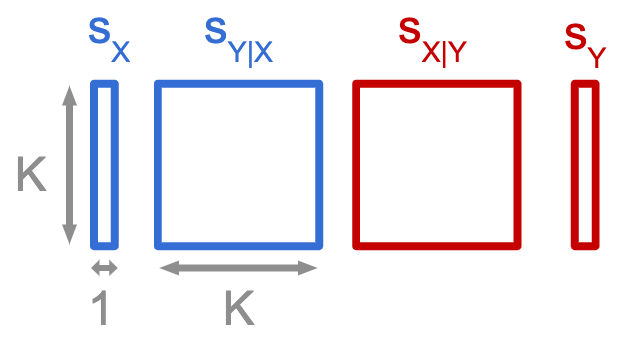
\includegraphics[width=.44\textwidth]{categorical_parameters.png}
    \caption{Parametrization of causal (blue) and anticausal (red) categorical models}
    \label{fig:categorical_models}
\end{wrapfigure}
Cause $X$ and effect $Y$ are now two categorical variables taking values in $\{1, \dots, K\}$.
Categorical variables are an exponential family with mean parameters $\vp\in\simplex_K$ the probability vector, and with natural parameter $\vs\in\real^K$ -- the logits or score parameters such that $\evp_z = \frac{e^{\evs_z}}{\sum_{z'} e^{\evs_{z'}}}$.
The causal model has parameters $\vs_X := (\evs_x)_{x=1\dots K}$ 
and $\vs_{Y|X} := (\evs_{y|x})_{x,y=1\dots K}$. 
We gather the causal parameters in the variable $\causalvar = (\vs_X, \vs_{Y|X})$ and the anticausal parameters in $\antivar = (\vs_Y, \vs_{X|Y})$ (Fig.~\ref{fig:categorical_models}).
The loss~\eqref{eq:causal_loss} becomes
\begin{align}
    &\cL_\text{causal}(\causalvar) 
    = \expect[(X,Y)\sim\ptransfer]{-\log \pmodel(X, Y)}\\
    &= \expect[\ptransfer]{- \evs_X + \log\sum_{x} e^{s_{x}} 
    - \evs_{Y|X} + \log\sum_y e^{s_{y|X}}}
    \; . \nonumber
\end{align}
Each mechanism's stochastic loss is the sum of a linear function and a softmax function.
The softmax function is convex and 1-Lipschitz, so we can apply rate~\eqref{eq:sgd_rate}. 
To be self-contained, we include details in Appendix~\ref{apdx:categorical_optimization}.

\subsection{Distance after Intervention}
\label{ssec:categorical_intervention_cause}
In this section, we prove that interventions on the cause advantage the causal model by a factor $K$, and we describe when interventions on the effect will advantage one model over another.

\paragraph{Intervention on cause $X$, } $\vs_X \assign \vs^*_X$.
The causal  conditional $\vs_{Y|X}$ is left unchanged,
but the effect marginal $\vs_Y$ is modified in a non-trivial way. 
Consequently the initial distances are 
\begin{align}
    &\delta_\text{causal} 
    = \|\vs_X - \vs^*_X\|^2 
    \\
    &\delta_\text{anticausal} 
    = \|\vs_Y - \vs^*_Y\|^2 
    + \sum_y \|\vs_{X|y} - \vs^*_{X|y}\|^2 \; .
\end{align}
The causal model has to update $K$ parameters, whereas the anticausal model has to adapt $K^2 + K$ parameters. Therefore the causal model seems to be advantaged by a factor $K$. The following proposition -- proved in  Appendix~\ref{apdx:categorical_analysis} -- shows that this is reflected by $\ell_2$ distances.
\begin{proposition}
\label{prop:categorical_cause}
When the intervention happens on the cause,
\begin{equation}
    \delta_\text{anticausal} \geq K \delta_\text{causal} \; .
\end{equation}
\end{proposition}

\begin{figure}
    \centering
    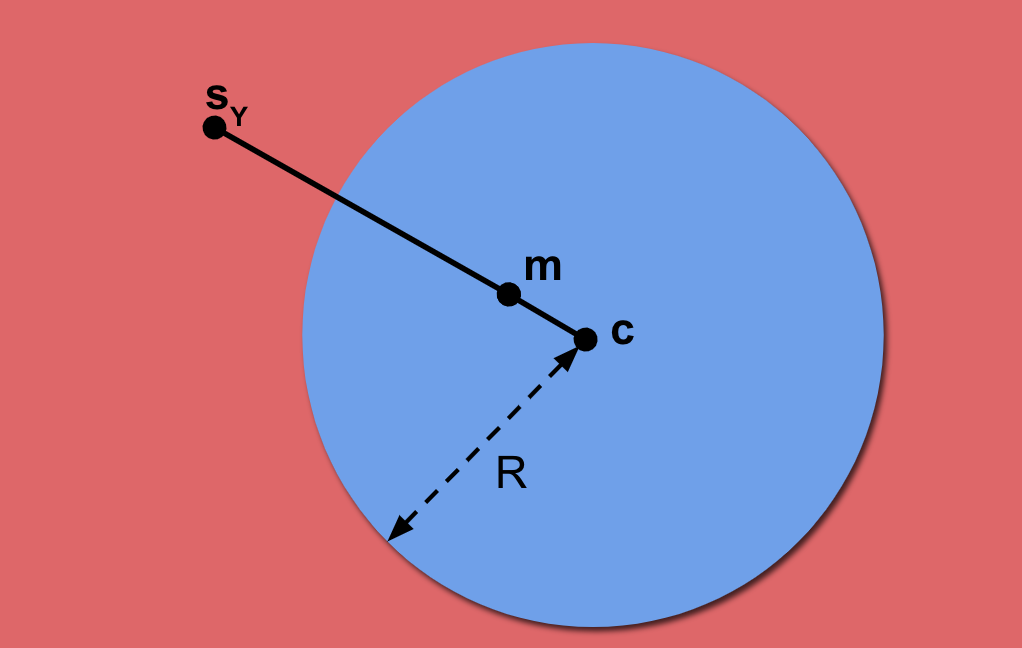
\includegraphics[width=.5\textwidth]{effect_sphere.png}
    \caption[Illustration of Proposition~\ref{prop:categorical_effect}]{
    \textbf{Illustration of Proposition~\ref{prop:categorical_effect}.}
    $\vc$ is on the line joining $\vs_Y$ and $\vm := \inv{K} \sum_x \vs_{Y|x}$. 
    When $\vs^*_Y$ is within the blue ball of radius $R$ centered at $\vc$, $\Delta \leq 0$ and the causal model is advantaged, otherwise the anticausal model is advantaged (red area). 
    This is a surprising counter-example to the adaptation-speed hypothesis.}
    \label{fig:effect_sphere}
\end{figure}

\paragraph{Intervention on effect $Y$, } $\forall x, \vs_{Y|x} \assign \vs^*_Y$.
Cause and effect become independent. 
The causal model is advantaged only if the intervention $\vs^*_Y$ is close enough from the previous marginal, as formalized by the following proposition:
\begin{proposition}
\label{prop:categorical_effect}
When the intervention happens on the effect
\begin{align}
    \Delta 
    &:= \delta_\text{causal} - \delta_\text{anticausal} \nonumber \\
    &= (K-1) \left(\norm{\vs^*_Y - \vc}^2 - R^2 \right)
\end{align}
where $R^2\approx K\widehat\Var_X[\log\sum_ye^{\evs_{y|X}}]$ 
and $\vc = \frac{\left(\sum_x \vs_{Y|x}\right) - \vs_Y }{K-1}$.
\end{proposition}
See Figure~\ref{fig:effect_sphere} for an illustration and Appendix~\ref{apdx:categorical_analysis_effect} for the exact formula of $R$ and the proof. 
When the intervention $\vs_Y^*$ is close enough to $\vc$, which depends on the reference, the causal model is advantaged. 
If $\vs_Y^*$ is far from $\vc$ or if $R$ is small then the anticausal model is likely to be advantaged.



\newlength{\hcolw}
\setlength{\hcolw}{0.32\textwidth}
\newlength{\scolw}
\setlength{\scolw}{0.1\textwidth}

\begin{figure*}[t]
    \centering
    \foreach \intervention in {cause,effect}{
        \foreach \plot in {scatter, curves}{
            \begin{subfigure}{\hcolw}
                \centering
                \includegraphics[width=\textwidth]{categorical/\plot_dense_\intervention_k=20.pdf}
                \caption{Dense - \intervention.}
                \label{fig:dense_\intervention_\plot}
            \end{subfigure}
        }
        \begin{subfigure}{\hcolw}
                \centering
                \includegraphics[width=\textwidth]{categorical/curves_sparse_\intervention_k=20.pdf}
                \caption{Sparse - \intervention.}
                \label{fig:sparse_\intervention_curves}
        \end{subfigure}
    }
    \caption[Experimental results on categorical data]{
    \textbf{Experimental results on categorical data.}
    Each plot is captioned with the prior and the intervention considered.
    \textbf{Scatter plots} are showing the positive correlation between the KL after 100 steps of SGD and the initial parameter distance. Each point represent one of 100 synthetic pairs $(\ptrue^{(0)},\ptrue^*)$.
    \textbf{Training curves} show the average KL (solid line) and the (5,95) percentiles (shaded) over 100 runs. Remark how all models start from the same initial KL, but they converge at different speeds.}
    \label{fig:categorical_results}
\end{figure*}




\subsection{Simulating Reference Distributions}
\label{sec:categorical_initialization}
To evaluate the fast adaptation criterion, we are going to work on synthetic data, which raises the question : from which distribution should we sample $\ptrue = \ptrue_{\theta^{(0)}}$? 
We call this distribution \emph{prior}.
Following the independent mechanism assumption, the marginal on the cause $\vp_X$ and  the conditional of effect given cause $\vp_{Y|X}$ should not contain any information about each other. 
\paragraph{Dense Prior.}
To sample causal mechanisms, a natural choice is
\begin{align}
    \label{eq:dense_prior}
    \vp_X \sim \Dir(\ones_K) 
    \quad \text{and} \quad
    \forall x, \vp_{Y|x} \sim \Dir(\ones_K)
\end{align}
where $\Dir$ is the Dirichlet distribution and $\ones_K$ is the all-one vector of dimension $K$.
$\Dir(\ones_K)$ the uniform law over the simplex $\simplex_K$.
% In~\eqref{eq:dense_prior}, we first sample a distribution from a uniform Dirichlet to generate the law of $X$. Then for each value of $X=x$, we sample a uniform Dirichlet to generate the law for the conditional $Y | X=x$.
This prior leads to the K2 score from the Bayesian network literature \citep{cooper1991bayesian}. 
We call this choice the \emph{dense prior} by opposition to the sparse prior introduced next.
This is the choice made in \citet{bengio2019meta}, as well as \citet{chalupka2016estimating}. 
The latter work reports that distributions sampled from this prior exhibit some asymmetry between $X$ and $Y$.
In Appendix~\ref{apdx:dense_prior}, we complement their work, explaining how the effect marginal is likely to be closer from the uniform distribution than the cause marginal.
This asymmetry means that \textit{the causal direction  is identifiable from observational data}.  

\paragraph{Sparse Prior.}
To fix this issue, we study an alternative prior that is symmetric and ensures that both cause and effect marginals are sampled from a uniform prior over $\simplex_K$. We sample the causal mechanisms as follows
\begin{align}
    \label{eq:sparse_prior}
    \vp_X \sim \Dir(\ones_K) 
    \quad \text{and} \quad
    \forall x, \vp_{Y|x} \sim \Dir(\ones_K /K) \; .
\end{align}
The $\ones_K /K$ parameter means that samples will be approximately sparse, hence the name.
We show in Appendix~\ref{apdx:sparse_prior} that with this sampling scheme, the joint is sampled from a sparse Dirichlet over $\simplex_{K^2}$: $\vp_{(X, Y)} \sim \Dir(\ones_{K^2} /K)$. 
This in turns means that we can switch the roles of $X$ and $Y$ in~\eqref{eq:sparse_prior}.
The effect marginal has uniform density over the simplex.
In general, \textit{the causal direction is not identifiable from observational data.}
In Bayesian Networks literature, this is known as the Bayesian Dirichlet equivalent uniform prior \citep{heckerman1995learning}.


\subsection{Categorical Variables Experiments}
\label{ssec:categorical_experiments}

\paragraph{Goal.}
As discussed in Section \ref{sec:categorical_initialization}, the prior over the joint distribution on $(X, Y)$ is going to influence the behavior of ASGD. 
We are seeking answers to two questions:
\begin{enumerate}
    \item Is the adaptation speed positively correlated with the initial distance, as suggested by the upper bound \eqref{eq:sgd_rate} on the convergence rate of ASGD?
    \item Is there a clear difference in adaptation speed between causal and anticausal models?
\end{enumerate}

\paragraph{Data.}
We consider categorical variables with $K =20$.
For each initialization method, we sample 100 different reference joint distributions. For each of these distributions, we sample an intervention by sampling a probability vector $\vq$ \textit{uniformly} from $\simplex_K$.
If the intervention is on the cause, we plug $\vq$ instead of $\vp_X$. 
If the intervention is on the effect, we redefine $\vp_{Y|x} = \vq, \forall x$.

\paragraph{Models.}
We are comparing causal and anticausal models adaptation speed. We also report results for a model of the joint 
$\vp_{X,Y} = \mathrm{softargmax}(\vs_{X,Y})$
as a reference model. We expect its results to be in between the performance of the causal and anticausal model as it expresses no prior over the direction. 
We optimize all models with Averaged SGD. In each iteration of SGD we get one fresh sample from the transfer distribution. For each model and each setting, we tune the (constant) learning rate so as to optimize the likelihood after seeing $\frac{K^2}{4}=100$ samples, to explore the few samples regime. 
We present results in Figure~\ref{fig:categorical_results}

%%%%%%%%%%%%%%%%%%%%%%%%%%%%%%%%%%%%%%%%%%%%%%%%%%%%%
\paragraph{Dense prior.}
% We report results with the dense prior in Figure~\ref{fig:dense_cause}.
When the intervention is on the cause, the causal model is much closer from its optimum: in Fig.~\ref{fig:dense_cause_scatter} the blue cluster is on the left of the scatter plots. 
This is well correlated with faster adaptation (Fig.~\ref{fig:dense_cause_curves}). 
On the contrary, \textit{when the intervention is on the effect, the anticausal model starts closer from its optimum} and it converges faster
(Fig.~\ref{fig:dense_effect_scatter}, \ref{fig:dense_effect_curves}).
We can interpret this result in light of Proposition~\ref{prop:categorical_effect}.
In Appendix~\ref{apdx:categorical_analysis_effect}, we explain why the radius $R$ is small under the dense prior.
As a result, $\vs_Y^*$ is mostly sampled outside of the ball of radius $R$, consequently the anticausal model is advantaged. 
Overall, there is a wider gap between models in  Fig.~\ref{fig:dense_cause_curves} than in Fig.~\ref{fig:dense_effect_curves}.
Consequently, if we take a balanced average of a few interventions on the cause and a few interventions on the effect, the causal model remains faster (details in Appendix~\ref{apdx:other_categorical_results}).


\paragraph{Sparse prior.}
When the intervention is on the cause, the causal model has a slight advantage (Fig.~\ref{fig:sparse_cause_curves}). 
When the intervention is on the effect, no model has a set advantage (Fig.~\ref{fig:sparse_effect_curves}), but the sparsity induces much higher KL values, as explained in Appendix~\ref{apdx:cat_sparse_explosion}.
This KL explosion drowns the signal coming from the cause intervention, calling for further algorithmic developments -- such as inferring the intervention, as explored by \citet{ke2019learning}.

%  _        _______  _______  _______  _______  _       
% ( (    /|(  ___  )(  ____ )(       )(  ___  )( \      
% |  \  ( || (   ) || (    )|| () () || (   ) || (      
% |   \ | || |   | || (____)|| || || || (___) || |      
% | (\ \) || |   | ||     __)| |(_)| ||  ___  || |      
% | | \   || |   | || (\ (   | |   | || (   ) || |      
% | )  \  || (___) || ) \ \__| )   ( || )   ( || (____/\
% |/    )_)(_______)|/   \__/|/     \||/     \|(_______/
\section{{Multivariate normal variables}}
In this section, we analyze the case of two multivariate normal variables with a linear relationship.
Cause $X$ and effect $Y$ are sampled from the causal model
\begin{align}
    \label{eq:normal_mean_model}
    & X \sim \cN(\mu_X, \Sigma_X)
   \\ % \quad \text{and} \quad
    & Y|X \sim \cN(\mA X + \va, \Sigma_{Y|X})
\end{align}
with mean parameters $\mu_X, \va \in \real^K$ and $\Sigma_X, \mA, \Sigma_{Y|X} \in \real^{K\times K}$.
This parametrization is the most intuitive but it is unfortunately not appropriate to get convergence rates.
We are going to introduce another parametrization  
along with an algorithm and a convergence rate (Sec.~\ref{ssec:proximal_gradient}),
before providing empirical results (Sec.~\ref{ssec:normal_experiments}).


\begin{figure*}[t]
    \centering
    \hskip 0.06\textwidth
    \foreach \name in {Natural Distance, Cholesky Distance, Speed vs Cholesky distance, Learning Curves}{
        \begin{minipage}{0.2\textwidth}
        \centering
        \name
        \end{minipage}
    }
    \foreach \intervention in {cause, effect}{
        \begin{minipage}{0.06\textwidth}
        \centering
        \intervention
        \end{minipage}
        \foreach \plottype in {distnat, distcho, scatter, curves}{
            \begin{subfigure}{0.2\textwidth}
            \centering
            \includegraphics[width=\textwidth]{normal/\plottype_\intervention_natural_k=10.pdf}
            \end{subfigure}
        }
    }
    \caption[Multivariate Normal Variables with dimension $K=10$]{
        \textbf{Multivariate Normal Variables with dimension $K=10$.}
        Row 1 and 2 correspond to interventions on cause and effect respectively.
        \emph{Column 1 \& 2:} scatter plot $\delta_\text{anticausal}$ vs $\delta_\text{causal}$ respectively in natural and Cholesky parametrization. The grey diagonal is the identity line.
        We observe a natural tendency for $\delta_\text{anticausal} > \delta_\text{causal}$ (points above the grey diagonal), but this is systematically true only for the natural distance when the intervention is on the cause.
        \emph{Column 3 \& 4:} same plot as in Figure~\ref{fig:categorical_results}. Once again we observe a correlation between initial distance and optimization speed. When the intervention is on the cause, the causal model is advantaged. 
        When the intervention is on the effect, both curves overlap.
    }
    \label{fig:normal_results}
\end{figure*}

\subsection{Optimization Analysis}
\label{ssec:proximal_gradient}
The negative log-likelihood of model~\eqref{eq:normal_mean_model} is notoriously non-convex. This is problematic for convergence results. 
For simplicity, we focus in this section on the simple marginal mechanism with mean parameters $\mu, \Sigma$. We detail the full model in Appendix~\ref{apdx:normal_analysis}.
If we use the natural parameters 
$\eta=\Sigma\iinv\mu$ and $\Lambda=\Sigma\iinv$ (precision matrix), the negative log-likelihood is convex
\begin{align}
    \label{eq:natgauss_nll}
    & \expect{- \log \ptrue_{(\eta, \Lambda)}(X)} \\
    &= \half \Big(
    \expect{\Tr (X X^\top \Lambda)  - 2 X^\top\eta}
    + \eta^\top \Lambda^{-1} \eta - \log{\abs{\Lambda}} \Big) \; . \nonumber
\end{align}
This objective is composed of a pleasant stochastic linear term,
and a difficult deterministic barrier objective which goes to infinity when $\Lambda \rightarrow 0$.
This barrier is composed of a matrix inverse and a log determinant.
The assumptions of Lipschitz or gradient-Lipschitz required to get SGD convergence do not hold for the barrier.
While the empirical version of~\eqref{eq:natgauss_nll} has a close formed formula for its global minimum, quite surprisingly, gradient-based optimization of the normal likelihood is difficult to analyze. 
Convex optimization typically deals with non-smooth terms by introducing proximal operators \citep{parikh2014proximal}. 
However this barrier term is too complex to get an analytic formula for the proximal operator.
We transform it into a more convenient form by introducing $\mL$, the lower triangular Cholesky factor of the precision matrix $\Lambda = \mL\mL^T$, and $\zeta = \mL^{-1} \eta = \mL^{\top} \mu$. 
Then~\eqref{eq:natgauss_nll} simplifies into
\begin{align}
    \label{eq:chogauss_nll}
    & \expect{ {-\log \ptrue_{(\zeta, \mL)}(X)} } \\
    & ={\half \expect{{\norm{\mL^\top X - \zeta}^2}} }
    {- \sum_i \log \mL_{i,i}} \; . \nonumber
\end{align}
We will refer to $(\zeta, \mL)$  as \emph{Cholesky parameters}.
This objective is more suitable to gradient based optimization with a simple proximal operator, as detailed in the next section. 
We provide all details about the causal model in Appendix~\ref{apdx:normal_analysis}.

\paragraph{Stochastic Proximal Gradient Algorithm}
We want to minimize the sum of a stochastic convex smooth function $f_X(\theta):=\half \norm{\mL^\top X - \zeta}^2 $ and convex non-smooth regularizer $g(\theta) = - \sum_i \log \mL_{i,i}$.
This is exactly the goal of the stochastic proximal gradient \citep{duchi2010composite} update
\begin{align}
    \label{eq:stochastic_prox_gradient}
    \!\!\! \theta_{t+1} = \argmin_\theta 
    g(\theta) + \inv{2\lr_t}\norm{
    \theta_t - \lr_t\nabla f_{X_t}(\theta_t) - \theta}^2
\end{align}
where~$\lr_t$ is the step-size and $X_t$ is randomly sampled.
For objective~\eqref{eq:chogauss_nll}, the proximal gradient update has a closed form solution that amounts to updating all parameters with the stochastic gradient of the quadratic term, then updating the diagonal elements of $\mL$ with the mapping $x \mapsto \half (x + \sqrt{x^2 + 4\lr})$, thus ensuring that they remain strictly positive (details in Appendix~\ref{apdx:normal_updates}).


\paragraph{Convergence Rate.}
We assume that stochastic gradients are almost-surely $\smoothness$-Lipschitz.
$\smoothness$ is known as the smoothness constant.
We show in Appendix~\ref{apdx:normal_conv_rate} that running the stochastic proximal gradient algorithm
with
step size $\lr_t = \frac{\lr}{3\smoothness \sqrt{T}}$ where $\lr\leq 1$, for $T$ iterations guarantees
\begin{equation}
    \expect{\KL(\ptrue^*||\ptrue_{\bar \theta^{(T)}}) }
    \leq \frac{3\smoothness \|\theta^{(0)} - \theta^*\|^2}{\lr \sqrt{T}}
    + \frac{ \KL(p^*||p_{\theta^{(0)}})}{T} \; .
    \label{eq:mirror_prox_rate}
\end{equation}



\paragraph{Analysis.}
The term $\nicefrac{ KL(p^*||p_{\theta^{(0)}})}{T}$ is equal for causal and anticausal models because we assume $\pmodel^{(0)} = \panti^{(0)}$.  
For normal variables, $\smoothness$ depends only on the data and is a priori equal for both models (Appendix~\ref{apdx:normal_constants}).
Similarly to \eqref{eq:sgd_rate}, both models' rates differ mainly by $\delta=\|\theta^{(0)} - \theta^*\|^2$.

When the intervention is on the cause, we prove in Appendix~\ref{apdx:normal_interventions} that the anticausal model is farther away from its optimum in the natural parametrization
\begin{align}
    \delta_\text{anticausal}^\text{natural} \geq  \delta_\text{causal}^\text{natural} \; . 
\end{align}
Unfortunately, in the Cholesky parametrization (Fig.~\ref{fig:normal_results}, 2nd column), or when the intervention is on the effect (Fig.~\ref{fig:normal_results}, bottom row),we observe empirically that there is no such hard guarantee, although the causal distance tends to be smaller than the anticausal distance.


\subsection{Experiments}
\label{ssec:normal_experiments}

Similarly to categorical variables, we need to decide on a prior over reference and transfer distributions. This choice is informed by two criteria.
First the independent mechanism principle which states that we should sample $\theta_X$ independently of $\theta_{Y|X}$.
Second we want $\theta_Y$ to have approximately the same distribution as $\theta_X$ 
-- e.g. we want the distribution to be approximately symmetric so that we cannot identify the direction from observational data. 
These considerations lead us to a flavor of normal-Wishart prior \citep{geiger2002parameter} described in Appendix~\ref{apdx:normal_experiments}.

We sample $100$ random joint distributions from this prior, and for each distribution we sample a random intervention on the cause, and a random intervention on the effect. We then run the stochastic proximal gradient on objective~\eqref{eq:chogauss_nll}. We report results in Figure~\ref{fig:normal_results}.
Similarly to the categorical case, when the intervention is on the cause, the causal model is advantaged by a slight margin (upper right figure). When the intervention is on the effect both models are learning at the same speed (bottom right figure).




\section*{Conclusion}
We provided a first theoretical analysis of the adaptation speed in two-variables cause-effect SCMs under localized interventions for categorical and normal data.
Convergence guarantees for stochastic optimization on the true population log-likelihood indicates that the adaptation speed is related to the distance between initial point and optimum in parameter space.
We verified this correlation empirically. 
We proved analytically that this distance is lower for the causal model than for the anticausal model when the intervention is on the cause variable.
This explains a surprising phenomenon: while both models start with the same suboptimality, one learns faster than the other.
When the intervention is on the effect variable, we highlighted examples showing that either model can be advantaged.
This observation challenges the intuition that the causal model should be the fastest to adapt, and it raises new questions for the approach of~\citet{bengio2019meta}, such as: are there practical situations where the fastest-to-adapt heuristic is useful ? 
On a more theoretical note, is it possible to characterize the adaptation speed behavior for more general families of distributions? 

%\bibliographystyle{abbrvnat}
%\bibliography{causal-optimization/references}

\clearpage
\newpage

\begin{subappendices}

\newcommand{\tet}{\theta_t}
\newcommand{\ttt}{\theta_{t+1}}
\newcommand{\ts}{\theta^{*}}

\onecolumn

\section{{Categorical optimization}}

In this section we prove a convergence rate of ASGD that applies to the categorical loss, and we show that the constants involved in this rate are the same for both causal and anticausal models.

\subsection{Convergence of ASGD with Fixed Step-Size}
\label{apdx:asgd_rate}
Here we derive a classical convergence rate of Average SGD.
This result is standard ; we include it to be self-contained.
The objective is 
\begin{align}
\min_{\theta} F(\theta) = \expect[i]{f(\theta,i)} \; .
\end{align}

\begin{theorem}
If each $f_i(\theta) = f(\theta,i)$ has bounded gradient $B$,
then after $T$ steps of SGD with step-size $\gamma=\frac{c}{\sqrt{T}}$,
starting from $\theta_0$,
the expected sub-optimality verifies
\begin{align}
   \expect{F(\bar{\theta}_T) - F(\ts)} \leq \frac{1}{2c\sqrt{T}}\|\theta_0- \ts\|^2 + \frac{ c B^2}{2\sqrt{T}}
\end{align}
where $\bar{\theta}_T = \frac{1}{T} \sum_t \tet$.
\end{theorem}

\begin{proof}
First we relate the $\ell^2$ distance to optimum at step $t+1$ with the one at step $t$ :
\begin{align*}
    &\| \ttt - \ts \|^2 \\
    &= \| \tet - \ts \|^2 - 2 \gamma \left < f'_i(\tet) , \tet-\ts \right> + \gamma^2\|f_i'(\tet)\|^2 \\
    &\leq \| \tet - \ts \|^2 - 2 \gamma \left < f'_i(\tet) , \tet-\ts \right> + \gamma^2B^2 \; .
\end{align*}
By convexity of $f_i$ and rearranging the terms we get 
\begin{align*}
2\gamma( f_i(\tet) - f_i(\ts) ) & \leq 2 \gamma \left < f'_i(\tet) , \tet-\ts \right> \\
& \leq  \| \tet - \ts \|^2 - \| \ttt - \ts \|^2+ \gamma^2B^2.
\end{align*}
Now we take the expectation, sum up both sides for $T$ iterations and divide by $2T\gamma$ to get
\begin{align*}
    &\frac{1}{T} \sum_{i=1}^T \expect{F(\tet) - F(\ts)} \\
    & \leq \frac{1}{2\gamma T}\left(\expect{\|\theta_0- \ts\|^2}
    - \expect{\|\theta_{T+1}- \ts\|^2}\right)
    + \frac{\gamma B^2}{2}\\
    & \leq \frac{1}{2\gamma T}\|\theta_0- \ts\|^2 + \frac{\gamma B^2}{2}
\end{align*}
Finally, we apply Jensen inequality to $F$ in $\bar{\theta}_T = \frac{1}{T} \sum_t \tet$
to get the final result.
\end{proof}

\subsection{Categorical Loss Properties}
\label{apdx:categorical_optimization}

We are now going to verify that assumptions of the rate \eqref{eq:sgd_rate} apply to the negative log-likelihood loss for the categorical distribution.
This loss is standard and it's properties are well-known, but we review them here to be self-contained.

Each mechanism has the same form of negative log-likelihood, with the same kind of stochastic gradients.
The total loss is a sum over mechanisms, and the total stochastic gradient is a concatenation of each mechanisms stochastic gradient.
To apply rate~\ref{eq:sgd_rate}, we can either apply it separately on each mechanism, either apply to the whole. Both path lead to the same result.
In the end, we simply have to check that this loss is convex, and has bounded gradients for all $z$.
The random functions coming from sampling $Z$ are 
\begin{equation}
    f_z(\vs) = -s_z + \log(\sum_{z'} e^{s_{z'}} )
\end{equation}
This function is the softmax -- or logsumexp -- function minus a  stochastic linear term. 

\paragraph{Convexity}
We are going to show that it is convex but not strongly convex because it becomes flat for large score values.
Its derivative is
\begin{equation}
    \nabla f_z(\vs) = -\ve_z + \vp \; .
\end{equation}
where $\ve_z$ is the $z$-th canonical basis element  and $\vp$ is the output of the softargmax function taken on $\vs_Z$.
The Hessian is the same for every $z$.
\begin{equation}
    \nabla^2 f_z(\vs) = \text{diag}(\vp) - \vp \vp^\top \; .
\end{equation}
We observe that for any vector $\vv$,
\begin{align}
    \label{eq:hessian2variance}
    \vv^\top \nabla^2 f_z(\vs) \vv &= \sum_z \evp_z\evv_z^2 - \left(\sum_z \evp_z \evv_z \right)^2 \nonumber \\
    &= \Var_{Z\sim \vp}[v_Z] \geq 0
\end{align}
which means that the logsumexp is convex. 
When $\evs_0$ tends toward positive infinity and the other components remain constant, $\vp$ tends toward a Dirac on the 0-th component.
Then \eqref{eq:hessian2variance} is 0 for all $\vv$, so the logsumexp is not strongly convex.

% \paragraph{Smoothness.}
% We can maximize \eqref{eq:hessian2variance} over the choice of $\vv$ in the unit ball and $\vp$ in the simplex to prove that the logsumexp is  $L=1/2$ smooth, and that this constant is reached for $\vp = (0.5, 0.5, 0, \dots )$ and $\vv=(-\frac{1}{\sqrt 2}, -\frac{1}{\sqrt 2}, 0, \dots )$. 

\paragraph{Bounded Gradients.}
The gradient norm is
\begin{align}
    \label{eq:cat_grd_uppr_bnd}
    \|\nabla f_z(\vs) \|
    &= \|\vp -\ve_z\| \\ \; .
\end{align}
This norm is maximized for $\vp=\ve_{z'}, \forall z' \neq z$.
The maximum is equal to $\sqrt{2}$.
If there are $d$ independent mechanisms (for $d$ variables in the graph), then the total stochastic gradient which is a concatenation of all gradients has a norm bounded by $B=\sqrt{2d}$. 
In our case of cause-effect models, $d=2$ and and the gradients are bounded by $B=2$, or in other words, all the $f_z$  are 2-Lipschitz.

This bound is the same for causal and anticausal models. It depends on the part of space where $\vp$ is going to live. Assuming that it is going to live in most of the space for both directed models, both loss will have the same Lipschitz constants in practice.

Thanks to these properties, the sample complexity of $\pmodel$ and $\panti$ are bounded by \eqref{eq:sgd_rate}. 
The difference in adaptation speed between causal and anticausal models is characterized by the distance in parameter space. 


% \subsection{Equality of gradient bound for both models}
% \label{apdx:categorical_constants}

% In this section we show that the stochastic gradient's norm upper bound which appears in the convergence term of ASGD in~\eqref{eq:sgd_rate} denoted by $B$ is the same for causal and anticausal models. Both marginals in causal and anticausal models have similar gradient form with different parametrizations $\vs_X$, and $\vs_Y \in \mathbb{R}^K$. Therefore to find $B$ for each marginal, we only need to solve the following supremum problem where $\vs$ is the parameter and $z$ is a sample
% \begin{equation}
%     \label{apdx:eq:marginal_gradient_bnd}
%     \sup_{z, \vs} \|\nabla_{\vs} f_z(\vs)\|^2 
%     = \|-\ve_z + \vp(\vs)\|^2  
%     \leq 2 \; . 
% \end{equation}
% For $\vs$ approaching infinity along axis $z'$, we have  $\vp=\ve_{z'}$. 
% If $z\neq z'$, then
% \begin{align*}
%     \sup_{z, \vs} \|\nabla_{\vs} f_z(\vs)\|^2 
%     \geq \|-\ve_z + \ve_{z'}\|^2= 2.  
% \end{align*}
% which is exactly equal to the upper bound for the gradient norm in~\eqref{eq:cat_grd_uppr_bnd}. With similar argument, the upper bound for the gradient magnitude of the conditional in both models is 2.  

\section{{Categorical analysis}}
\label{apdx:categorical_analysis}

In this section, we prove relationships between parameter distances induced by interventions between the causal and anticausal models. 
First we prove two useful lemmas. 
Then we establish that the causal model dominates the anticausal model by a factor $K$ when the intervention is on the cause. 
Finally we show that no model has a set advantage when the intervention bears on the effect.


The logits or scores $\vs$ live in $\real^K$.
They have one additional degree of freedom compared to the probability $\vp$. 
More specifically, the softargmax is invariant by translations along the vector $\ones = (1,\dots, 1)$.
In other words, all scores $\{ \vs + \lambda \ones | \forall \lambda \in \real \}$ are equivalent. 
Scores which move by following the gradient of this loss will remain in the same affine hyperplane orthogonal to $\ones$.
To ensure that the distances we measure are meaningful, we project all logits in the hyperplane such that $\sum_z \evs_z = 0$, by subtracting their mean.
% \begin{align}
%     \vs \assign \vs - (\frac{1}{K}\sum_z \evs_z) \ones
% \end{align}
\begin{definition}[Mean-zero score]
\label{def:mean_zero}
A score vector $\vs$ is mean-zero iff $\sum_z \evs_z = 0$.
\end{definition}


\subsection{Switching Direction}
In this section we are going to prove a few useful results relating cause and anticausal models.
We know the causal parameters $X \rightarrow Y$, and we want to find the corresponding $X \leftarrow Y$ model,
e.g. express $\vs_Y, \vs_{X|Y}$ as a function of $\vs_X, \vs_{Y|X}$ .
This will help us to find a relationship between $\delta_\text{causal}$ and $\delta_\text{anticausal}$.
We first need to define a few useful variables
\begin{definition}[Average conditional score vectors]
\label{def:average_conditional_logit}
For any $x$ or $y$, define
\begin{align}
    \mm(y):= \frac{1}{K} \sum_x \evs_{y|x}, \quad
    \nn(x):= \frac{1}{K} \sum_y \evs_{x|y} \; .
\end{align}
\end{definition}
\begin{definition}[Conditional log-partition function]
    \begin{align}
        \logpartition(x) = \log \sum_y e^{\evs_{y|x}}
    \end{align}
\end{definition}
With these variables, we can express the reverse conditional score from the causal parameters.
\begin{lemma}[Anticausal conditional score]
\label{lem:categorical_reverse}
Let $\evs_{y},\evs_{x}$ be marginal scores, 
and $\evs_{y|x},$ $\evs_{x|y}$ be conditional scores. Then
\begin{equation}
    \label{eq:bayes_scores}
    \boxed{\evs_{x|y} = \evs_x + (\evs_{y|x} - \mm(y)) - (\logpartition(x) - \alpin)} \; ,
\end{equation}
where $\alpin = \frac{1}{K} \sum_x \logpartition(x)$.
\end{lemma}

\begin{proof}
Let's apply Bayes rule to find the conditional probability mass function
\begin{align*}
    \ptrue(x|y) 
    &\propto \ptrue(y|x) \ptrue(x) \\
    &\propto \exp \left(\evs_{y|x} - \logpartition(x)
    + \evs_x\right)
\end{align*}
where $\logpartition(x)$ is the log-partition function of $\ptrue(y|x)$.
Taking the logarithm, 
\begin{equation}
    \label{eq:un_condx}
    \evs_{x|y} = \evs_x + \evs_{y|x} - \logpartition(x) + C(y)
\end{equation}
where $C(y)$ is a constant defined such that $\sum_x \vs_{x|y} = 0$ (see Definition~\ref{def:mean_zero}).
%We can safely ignore the log-partition of $\ptrue(x)$ because it is a constant that will disappear in the normalization.
We take the sum of~\eqref{eq:un_condx} over $x$ to find
\begin{align*}
    & &\sum_x \evs_x& + &\sum_x \evs_{y|x}& - &\sum_x\logpartition(x)& + &K C(y)\\
    &= &0& + &K\mm(y)& + &K\alpin& +  &K C(y)
\end{align*}
which simplifies into
\begin{align*}
    C(y) = - \mm(y) - \alpin
\end{align*}
We plug this in~\eqref{eq:un_condx} to conclude the proof.
\end{proof}

%
We conclude this section with an identity showing that conditional logits are equally close from their averages in both directions.
\begin{lemma}
\label{lem:categorical_identity}
For any $x$ and $y$ we have 
\begin{equation}
    \label{eq:scores_identity}
    \boxed{\evs_{x|y} - \nn(x) = \evs_{y|x} - \mm(y)} \;.
\end{equation}
where $\nn(x):= \frac{1}{K} \sum_y \evs_{x|y}$ and $\mm(y):= \frac{1}{K} \sum_x \evs_{y|x}$. 
\end{lemma}

\begin{proof}
We apply Lemma~\ref{lem:categorical_reverse} with the roles of $X$ and $Y$ inverted to express $\vs_{y|x}$ as a function of the anti  causal parameters
\begin{align}
\label{eq:bayes_scores_anti}
    \evs_{y|x} &= \evs_y + (\evs_{x|y} - \nn(x)) - (\logpartitionb(y) - \betin) \; ,
\end{align}
where
$\logpartitionb(y) = \log \sum_x e^{\evs_{y|x}}$ 
and $\betin = \frac{1}{K} \sum_y \logpartitionb(y)$.
We can add \eqref{eq:bayes_scores} and \eqref{eq:bayes_scores_anti} 
to get rid of the conditional scores 
\begin{align*}
    \evs_x - \nn(x) - \logpartition(x) + \alpin
    = - (\evs_y - \mm(y) - \logpartitionb(y) + \betin), 
\end{align*}
for all $x,y$.
The left hand side is constant in $y$ whereas the right hand side is constant in $x$. 
Thus both sides are constants with respect to both $x$ and $y$. 
In particular they are equal to their average
\begin{align*}
    \forall x, 
    \evs_x - \nn(x) - \logpartition(x) + \alpin
    &= \inv{K} \sum_{x'} (\evs_{x'} - \nn(x'))\\
    &-\inv{K} \sum_{x'} \logpartition(x') + \alpin \\
    &= 0 - 0 - \alpin + \alpin \\
    &= 0 \; .
\end{align*}
We plug this equality into \eqref{eq:bayes_scores} to prove the lemma.
\end{proof}


\subsection{Intervention on Cause}
\label{apdx:categorical_analysis_cause}
In this section, we analyze the relationship between $\delta_\text{causal}$ and $\delta_\text{anticausal}$ after an intervention on the cause. 

\paragraph{Proposition~\ref{prop:categorical_cause}.}
\begin{itshape}
{If an intervention happens on the cause $X$ then we have}
\begin{equation}
    \boxed{
    \delta_\text{anticausal} \geq K \delta_\text{causal}} \; ,
\end{equation}
where $\delta_\text{causal} = \|\vs_X - \vs^*_X\|^2$, and $\delta_\text{anticausal} = \|\vs_Y - \vs^*_Y\|^2  + \sum_y \|\vs_{X|y} - \vs^*_{X|y}\|^2$
\end{itshape}
     


\begin{proof}
Given that $\evs^*_{y|x} = \evs_{y|x}, \vm^* = \vm, \logpartition^*=\logpartition$ and $\alpin^*=\alpin$,  Lemma~\ref{lem:categorical_reverse} tells us that the anticausal conditional $\vs^*_{X|Y}$ verifies
\begin{align*}
    \evs^*_{x|y} - \evs^*_x 
    = (\evs_{y|x} - \mm(y)) - (\logpartition(x) - \alpin)
    = \evs_{x|y} - \evs_x \\
    \implies
    \evs_{x|y} - \evs^*_{x|y}  
    = \evs_x  -\evs^*_x  \; .
\end{align*}
The distance between models before and after intervention are
\begin{align*}
    \delta_\text{causal}
    &= \|\vs_X - \vs^*_X\|^2 \\
    \delta_\text{anticausal}
    & = \|\vs_Y - \vs^*_Y\|^2  + \sum_y \|\vs_{X|y} - \vs^*_{X|y}\|^2 \\
    & \geq 0 +  \sum_y \sum_x ( \evs_x - \evs^*_{x})^2 = K \|\vs_X - \vs^*_X\|^2 \;.
\end{align*}
In conclusion,
\begin{equation}
    \delta_\text{anticausal} \geq K \delta_\text{causal} \; .
\end{equation}
\end{proof}

\subsection{Intervention on Effect}
\label{apdx:categorical_analysis_effect}
The following proposition shows that when the intervention is on the effect, the causal model is advantaged only when the new effect marginal $\vs^*_Y$ is close enough from the previous marginal. 

\paragraph{Proposition~\ref{prop:categorical_effect}}
\begin{itshape}
 When an intervention happens on the effect
\begin{align}
    \label{eq:categorical_effect_distdiff}
    \Delta 
    :&= \delta_\text{causal} - \delta_\text{anticausal}\\
    &= (K-1) \left(\norm{\vs^*_Y - \vc}^2 - R^2\right)
\end{align}
where the score vector $\vc$ and the scalar $R$ are defined as
\begin{align}
    \vc =& \frac{K\vm - \vs_Y }{K-1} \\
    (K-1) R^2 =& K  \|\vn - \vs_X \|^2  + (K-1) \norm{\vc}^2 \\
    & + \norm{\vs_Y}^2 - K\norm{\vm}^2 \nonumber
\end{align}
with $\vm$ and $\vn$ as in Definition~\ref{def:average_conditional_logit}.
\end{itshape}

We illustrate the relationship between $\vm$, $\vc$, $\vs_Y$  and $R$ in Figure~\ref{fig:categorical_sketch_effect}. 

\begin{figure}
    \centering
    \begin{subfigure}{0.45\textwidth}
    \centering
    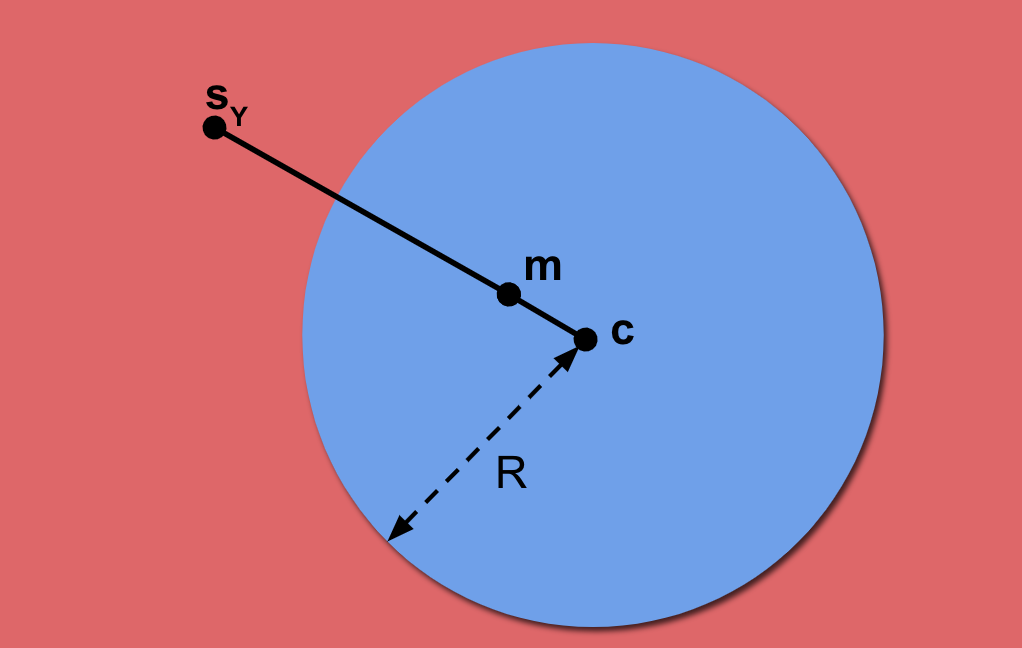
\includegraphics[width=.9\columnwidth]{effect_sphere.png}
    \caption{
    $\vm$ is a convex combination of $\vc$ and $\vs_Y$. 
    The blue bubble is the sub-level set 0 of $\Delta$.
    It is a circle of radius $R$ centered at $\vc$.
    Within this circle, $\delta_\text{causal} \leq \delta_\text{anticausal}$  the causal model is advantaged. 
    Outside this circle, $\delta_\text{causal} \geq \delta_\text{anticausal}$ the anticausal model is advantaged.}
    \label{fig:categorical_sketch_effect}
    \end{subfigure}
    \quad \quad
    \begin{subfigure}{0.45\textwidth}
    \centering
    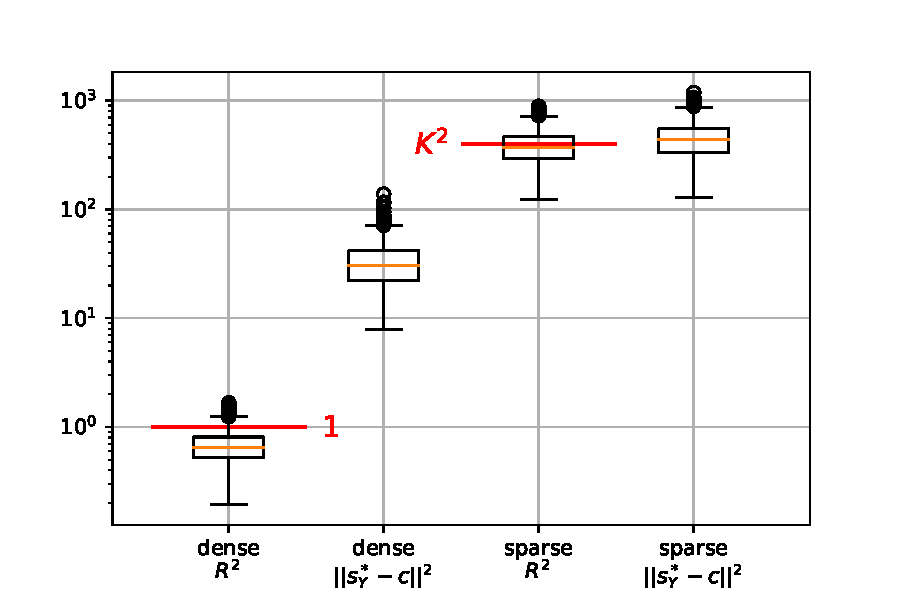
\includegraphics[width=\columnwidth]{categorical_effect_distance.pdf}
    \caption{
    Box plots for the radius $R^2$ and deviations $\|\vs_Y^* - \vc\|^2$ for $K=20$ with the dense prior (left) and the sparse prior (right). 
    The y-axis is logarithmic.
    Red lines show analytical estimates for the expected radius.
    }
    \label{fig:radius_boxplot}
    \end{subfigure}
    \caption{Behavior of the hyper-sphere within which the causal model is advantaged, as presented in Proposition~\ref{prop:categorical_effect}.}
    \label{fig:radius_illustrations}
\end{figure}

\begin{proof}
First we expand the causal distance with a bias variance decomposition
\begin{align}
    \delta_\text{causal} 
    &= \sum_x \|\vs_{Y|x} - \vs^*_Y \|^2 \nonumber\\
    &= \sum_{x,y} (\evs_{y|x} - \mm(y) + \mm(y)- \evs^*_y )^2 \nonumber\\
    &= \textcolor{blue}{\sum_{x,y} (\evs_{y|x} - \mm(y))^2 } 
    +K \sum_y ( \mm(y)- \evs^*_y )^2 
    \label{eq:categorical_effect_causal} \nonumber\\
    & \quad + 2\sum_y (\mm(y)- \evs^*_y ) \underbrace{\sum_x (\evs_{y|x} - \mm(y))}_{=0} \; . 
\end{align}
Given that $\vs^*_{X|y} = \vs_{X}$, we can decompose the anticausal distance similarly
\begin{align}
    \delta_\text{anticausal} 
    &= \|\vs_Y - \vs^*_Y \|^2 + \sum_y \| \vs_{X|y} - \vs^*_{X|y}\|^2 \nonumber\\
    &= \|\vs_Y - \vs^*_Y \|^2 + \sum_{x,y}  (\evs_{x|y} - \nn(x) + \nn(x) - \evs_x )^2\nonumber \\
    &= \|\vs_Y - \vs^*_Y \|^2 
    + \textcolor{blue}{\sum_{x,y}  (\evs_{x|y} - \nn(x))^2}\nonumber\\ 
    &+  K \sum_x (\nn(x) - \evs_x )^2 
    \label{eq:categorical_effect_anticausal}\; .
\end{align}
Thanks to Lemma~\ref{lem:categorical_identity}, the variance of conditional score vectors (in blue) in \eqref{eq:categorical_effect_causal} and \eqref{eq:categorical_effect_anticausal} are equal
\begin{align*}
 \textcolor{blue}{\sum_{x,y}  (\evs_{x|y} - \nn(x))^2 
 = \sum_{x,y} (\evs_{y|x} - \mm(y))^2} \; .
\end{align*}
What remains in the difference is the quadratic form
\begin{align*}
    \Delta 
    &= \delta_\text{causal} - \delta_\text{anticausal} \\
    &=  K \|\vm - \vs^*_Y\|^2  
    - K\|\vn - \vs_X \|^2
    - \| \vs_Y - \vs^*_Y \|^2 \; ,
\end{align*}
which we can expand to highlight the role of $\vs^*_Y$ as
\begin{align*}
    \Delta
    =& (K-1) \|\vs^*_Y\|^2
    - 2 \langle \vs^*_Y, K\vm - \vs_Y \rangle \\
    & + K\|\vm\|^2  - \|\vs_Y\|^2 
    - K\|\vn - \vs_X\|^2 \|^2 \\
    =& (K-1) \|\vs^*_Y - \vc\|^2
    - (K-1) \|\vc\|^2 \\
    & + K\|\vm\|^2  - \|\vs_Y\|^2 
    - K\|\vn - \vs_X\|^2 
\end{align*}
where $\vc$ appears as a non-convex interpolation of $\vm$ and $\vs_Y$, 
$\vc = \frac{K\vm - \vs_Y }{K-1}$. 
Define $R^2$ to conclude the proof.
\end{proof}


\paragraph{Empirical estimates of the radius.}
We report values of $R^2$ and $\norm{\vs_Y^* - \vc}^2$ observed for the dense and sparse priors in Figure~\ref{fig:radius_boxplot}.
For dense prior radii are much smaller than  deviations, whereas for the sparse prior they have similar magnitude. 
This explains why the anticausal model systematically adapts faster when the intervention is on the effect and the prior is dense. 
We also observe that radii (and deviations)  are much greater for the sparse prior than for the dense prior.
In the following paragraph we provide some clues  to explain this behaviour.

As illustrated by Figure~\ref{fig:categorical_sketch_effect}, $\vm$ is a convex combination of $\vc$ and $\vs_Y$ : $\vm = \frac{(K-1)\vc + \vs_Y}{K}$ so by convexity of $\|.\|^2$,
\begin{align*}
    &\frac{K-1}{K} \|\vc\|^2 + \inv{K}\|\vs_Y\|^2  \geq \|\vm\|^2 \\
    \implies &(K-1) \|\vc\|^2 + \|\vs_Y\|^2  -K \|\vm\|^2  \geq 0 \\
    \implies &R^2 \geq \|\vn - \vs_X \|^2 \; .
\end{align*}
As $K$ grows larger, this inequality will get closer and closer to an equality. Indeed, $\vm$ will get closer and closer to $\vc$ and we will end up with 
\begin{align*}
    \frac{K-1}{K} \|\vc\|^2 + \inv{K}\|\vs_Y\|^2  - \|\vm\|^2 \ll \|\vn - \vs_X \|^2 \approx R^2 \; .
\end{align*}
Before proceeding, let us prove a simple proposition that is a direct consequence of Lemma~\ref{lem:categorical_reverse}.
\begin{proposition}
\label{prop:marginal_and_average_conditional}
The squared distance between marginal score and reverse average conditional is equal to the empirical variance of the conditional log-partition function
\begin{equation}
    \norm{\vs_X - \vn}^2 = K \widehat\Var_X[\logpartition(X)] \; .
\end{equation}
\end{proposition}
\begin{proof}
Taking the average of Lemma~\ref{lem:categorical_reverse} over $y$ yields
\begin{align*}
    \inv{K}\sum_y \evs_{x|y} 
    &= \evs_x - (\logpartition(x) - \alpin) + \inv{K}\sum_y (\evs_{y|x} - \mm(y))  \\
    \nn(x) 
    &= \evs_x - (\logpartition(x) - \alpin)\; ,
\end{align*}
where we used the definition of $\nn(x)$ and the mean-zero scores. 
Reordering terms gives
\begin{equation}
    \evs_x - \nn(x) =  \logpartition(x) - \alpin \;
\end{equation}
Recall that $\alpin$ is the average of $\logpartition(x)$ over $x$. 
Squaring this equation and summing over $x$ concludes the proof.
\end{proof}

Using this proposition we get that 
\begin{align*}
    R^2 &\approx \norm{\vs_X - \vn}^2 \\
    &= K \widehat\Var_X[\logpartition(X)] \\
    & = K \widehat\Var_X[\log\sum_y e^{\evs_{y|X}}]
    %\implies R &\approx \sqrt{K} \widehat\Std_X[\log\sum_y e^{\evs_{y|X}}]
    \; .
\end{align*}
Conditional scores $\vs_{y|x}$ are taking much greater values with much higher variance under the sparse prior than under the dense prior.
To be clear, we sample independently pseudo-scores $\tilde \evs_{y|x}$ from exp-gamma laws, and we subtract their mean to ensure that they sum to 0 (Definition~\ref{def:mean_zero}). 
$\evs_{y|x} = \tilde \evs_{y|x} - \inv{K} \sum_{y'} \tilde \evs_{y'|x} $.
This means that
\begin{align*}
    \log\sum_y e^{\evs_{y|X}} = \log\sum_y e^{\tilde \evs_{y|X}} 
    - \inv{K} \sum_{y} \tilde \evs_{y|x}
\end{align*}
If we make the approximation that the logsumexp term and the average term are independent then
\begin{align*}
    &\widehat\Var_X[\log\sum_y e^{\evs_{y|X}}] \\
    &\approx \Var_{\evs_{y|x}}[\log\sum_y e^{\evs_{y|x}}] \\
    &\approx \Var_{\tilde\evs_{y|x}}[\log\sum_y e^{\tilde \evs_{y|X}}]
    + \inv{K} \Var_{\tilde\evs_{y|x}}[\sum_{y} \tilde \evs_{y|x}] \\
    & = \psi^{(1)}(K\lambda) +  \inv{K}\psi^{(1)}(\lambda)
\end{align*}
where this last step uses the formula for the variance of an exp-gamma variable twice. 
The variance of an exponential gamma with shape parameter $\lambda$ is $\psi^{(1)}(\lambda)$ where $\psi^{(1)}$ is the trigamma function. 
The log-sum-exp of $K$ independent exp-gamma with scale and shape parameters $(\lambda, \zeta)$ is another exp-gamma with scale and shape parameters $(K \lambda, \zeta)$.
Finally we get the following approximation for the squared radius
\begin{align*}
    R^2 \approx K \psi^{(1)}(K\lambda) + \psi^{(1)}(\lambda) \; .
\end{align*}
The dense prior uses a shape parameter $\lambda=1$ while the sparse prior uses a shape parameter $\lambda=\inv{K}$.
We use two approximations of the trigamma function: $\psi^{(1)}(\inv{K})\approx K^2 + \pi^2/6$  and $\psi^{(1)}(K)\approx \inv{K}$ when $K\geq 10$.
\begin{align*}
    R^2_\text{dense} 
    &\approx K \psi^{(1)}(K) + \psi^{(1)}(1) \\
    &\approx 1 + \pi^2/6  = O(1)\\
    R^2_\text{sparse} 
    &\approx K \psi^{(1)}(1) + \psi^{(1)}(\inv{K}) \\
    &\approx K^2 + K \pi^2 /6 +  \pi^2 /6  = O(K^2) \; .
\end{align*}
In other words for dense prior the radius grows linearly with the dimension $K$. We report these estimates along with real data in Figure~\ref{fig:radius_boxplot}.


\paragraph{Independent Special Case.} 
if $X$ is independent of  $Y$ in the reference distribution -- e.g. $\forall x, y, \ptrue(x, y) = \ptrue(x) \ptrue(y)$ -- then $\forall x, y,$
\begin{align*}
    \evs_x &= \evs_{x|y} = \nn(x) \\
    \evs_y &= \evs_{y|x} = \mm(y)
\end{align*}
Plugging these equalities into Proposition~\ref{prop:categorical_effect} yields
\begin{align*}
    \vc &= \vm = \vs_Y 
    \quad \text{and} \quad
    R = 0 \\ 
    \implies 
    \Delta &=  (K-1) \norm{\vs^*_Y - \vs_Y}^2 
    \geq 0
\end{align*}
which means that the anticausal model is advantaged
$\delta_\text{causal} \geq \delta_\text{anticausal}$. 
This is actually predictable from a simple parameter counting argument. 
When the reference distribution is made of independent distributions, the anticausal conditional mechanism is already optimal $\evs_x = \evs_{x|y}$.
The anticausal model only has to adapt its marginal mechanism $\vs_Y$ of size $K$.
On contrary, the causal model only has to adapt its conditional mechanism $\evs_{y|x} \neq \evs_y$ of size $K^2$.
Overall the causal model has to adapt $K$ times more parameters than the anticausal model.

\subsection{Other Empirical Results for Cause and Effect Interventions}
\label{apdx:other_categorical_results}

In this section, we present additional results for categorical variables.
In Figure~\ref{fig:dense_results}, compared to the main text, we add what happens with the dense prior when we average learning curves (pooled) from 5 interventions on the cause and 5 interventions on the effect : on average the causal model adapts the fastest.
In Figure~\ref{fig:sparse_results}, compared to the main text we show what happens with the sparse prior, both in terms of distance (scatter plots) and in terms of pooled results. Because the intervention on the effect creates huge values of the KL, there is no set advantage for any of the models. 

% DENSE
\begin{figure*}
    \centering
    \foreach \intervention in {cause,effect,pooled}{
        \begin{minipage}{0.3\textwidth}
         \centering
            Dense \intervention
        \end{minipage}
    }    
        \foreach \plot in {curves, scatter}{
         \foreach \intervention in {cause,effect,pooled}{
            \begin{subfigure}{0.3\textwidth}
                \centering
                \includegraphics[width=\textwidth]{categorical_dense/\plot_\intervention_k=20.pdf}
            \end{subfigure}
        }
    }
    \caption[Categorical dense prior with K=20]{
        \textbf{Categorical dense prior with K=20.}
        \textit{Row 1:} training curves. Solid lines are average KL over 100 runs. We tune hyper-parameters to minimize the average KL of each model at the black vertical dashed bar ($t$=100). Shaded areas are between (5,95) quantiles. Note that \textit{all models start from the same initial KL, but they converge at different speeds.}
        \textit{Row 2:} scatter plot of the KL at $t$=100 vs. initial distance. Note that the initial distance is well correlated with the KL after 100 steps of SGD.
        \textit{Columns:} we report results for interventions on the cause on column 1, the effect on column 2, and an aggregation of both on column 3. We aggregate results by taking the average of 5 cause interventions and 5 effect interventions as one new trajectory. In total we have 20 such trajectories per model. We are reporting this result because the meta-learning criterion suggested by \citet{bengio2019meta} is akin to the average adaptation speed over a small set of interventions. 
    }
    \label{fig:dense_results}
\end{figure*}

% SPARSE
\begin{figure*}
    \centering
    \foreach \intervention in {cause,effect,pooled}{
        \begin{minipage}{0.3\textwidth}
         \centering
            Sparse \intervention
        \end{minipage}
    }
    \foreach \plot in {curves, scatter}{
        \foreach \intervention in {cause,effect,pooled}{
            \begin{subfigure}{0.3\textwidth}
                \centering
                \includegraphics[width=\textwidth]{categorical_sparse/\plot_\intervention_k=20.pdf}
            \end{subfigure}
        }
    }
    \caption[Categorical sparse prior with K=20]{
        \textbf{Categorical sparse prior with K=20.}
        \emph{Column 1:} intervention on the cause. The causal model starts closer from optimum and adapts slightly faster than others.
        \emph{Column 2:} intervention on the effect. All models have the same initial distance and the same objective value. However the KL value is around 10. This is 10 times larger than when the intervention is on the cause.
        \emph{Column 3:} we take the average of 5 effect and 5 cause interventions. The effect dominates this average because it is much larger. As a result there is no signal.
    }
    \label{fig:sparse_results}
\end{figure*}


\subsection{Single Mechanism Intervention}
If only $\vs_{Y|x_0}$ changes, for some $x_0$, then from Lemma~\ref{lem:categorical_reverse} we get the following equality
\begin{align}
    \label{eq:single_mechanism}
    \delta_\text{anticausal} =
    &\frac{K-1}{K}\delta_\text{causal}
    + \norm{\vs_Y^* - \vs_Y}^2  \nonumber\\
    &+ (K-1)(\logpartition^*(x_0) - \logpartition(x_0))^2 \; .
\end{align}
The causal and anticausal distances seem to be on the same scale, with a multiplicative factor $\frac{K-1}{K} \lessapprox 1$ and a positive additive factor.
This is interesting because the sparsity argument holds: the causal model needs to change $K$ parameters whereas the anticausal model needs to change $K^2+K$ parameters.
That means we could expect an advantage by a factor $K$ for the causal model, similarly to when the intervention is on the cause.
However \eqref{eq:single_mechanism} tells another story: without further assumptions, it seems like both distances will have the same scale.

\begin{figure}
    \centering
    \foreach \init in {dense,sparse}{
        \foreach \plot in {curves, scatter}{
        \init 
            \begin{subfigure}{.4\textwidth}
                \centering
                \includegraphics[width=\textwidth]{categorical_\init/\plot_singlecond_k=20.pdf}
            \end{subfigure}
        }
    }
    \caption[Single mechanism intervention with K=20]{
        \textbf{Single mechanism intervention with K=20.}
        \emph{Two first rows:} Dense prior. The only model to be slightly advantaged is the joint model. 
        \emph{Two last rows:} Sparse prior. This time there is a slight advantage for the causal model which performs comparably to the joint model.
        Overall the optimization is hard in both settings, since we are observing only $K^2$ samples for models with $O(K^2)$ parameters. The KL barely decreases.
    }
    \label{fig:single_mechanism_intervention}
\end{figure}

\paragraph{Experiments.}
For this kind of intervention to be detectable, we need to intervene on $x_0$ such that $\ptrue(x_0)$ is quite large. 
To ensure this in our experiments, we pick $x_0 = \argmax_x \ptrue(x)$. We report results on dense and sparse priors in Figure~\ref{fig:single_mechanism_intervention}. 
We observe no significant advantage for the causal model, in spite of the parameter counting prediction.

\section{{Categorical priors}}
In this section we study the dense and sparse prior described in the main paper.

\subsection{Causal Direction is Identifiable under the  Dense Prior}
\label{apdx:dense_prior}

\citet{chalupka2016estimating} study the prediction of causal direction from observational data under the dense prior assumption. 
The causal direction $X \rightarrow Y$ induces a certain prior over joint distributions $\pi(\vp | \rightarrow)$.  
The anticausal direction $X \leftarrow Y$ induces another one $\pi(\vp | \leftarrow)$.
The Bayes classifier is predicting $\rightarrow$ if 
\begin{align}
    \label{eq:bayes_classifier}
    \log\pi( \rightarrow | \vp) -  \log\pi( \leftarrow | \vp) > 0 \; ,
\end{align}
and $\leftarrow$ otherwise.
Under the dense prior assumption, this classifier makes an error of approximately $0.4$ for $K=2$, which decreases exponentially to $0.001$ for $K=10$.
We reproduced their setting and report the error of the optimal classifier in Table \ref{tab:chalupka_error} for varying K.
In other words the dense prior induce very asymmetric distributions which makes the causal direction identifiable. 

Is this Bayes classifier easy to estimate ? 
It turns out that under the dense prior, the criterion~\eqref{eq:bayes_classifier} can be simplified into the following criterion   
\begin{align}
    \label{eq:chalupka_criterion}
    \KL(\uniform || \ptrue_X) - \KL(\uniform || \ptrue_Y) > 0
\end{align}
where $\uniform := \ones / K$ is the uniform probability vector.
The proof is left as an exercize to the reader. 
If \eqref{eq:chalupka_criterion} is positive, Bayes predicts that the cause is $X$, otherwise $Y$ is the cause.
In words, whichever variable has the most uniform marginal is the effect.
This simple rule is optimal given the prior assumption (and if both directions are equally likely).
We can understand it from a concentration of measure perspective.
The effect marginal is written as a sum of quasi independent uniform variables
\begin{equation}
    \ptrue(y) = \sum_x \ptrue(y|x) \ptrue(x)
\end{equation}
which ends up close from the uniform vector.

\begin{table*}[]
    \small
    \centering
    \begin{tabular}{c|cccccccccccccc}
        K & 2 & 3 & 4 & 5 & 6 & 7 & 8 & 9 & 10 & 11 & 12 & 13 & 14 \\
        \toprule
        error & .4 & .2 & .1 & .07 & .03 & .01 & .005 & .002 & .0007 & .0003 & 7e-5 & 3e-5 & 4e-6 
    \end{tabular}
    \caption[Estimation of the Bayes error under the dense prior assumption]{Estimation of the Bayes error under the dense prior assumption for increasing categorical variables dimension K. 
    We estimated these numbers by sampling one million joint distributions for each K. We report 1 significant figure.}
    \label{tab:chalupka_error}
\end{table*}


\subsection{Joint Distribution with Sparse Prior}
\label{apdx:sparse_prior}

The following theorem shows how a Dirichlet prior over joint distributions $\evc_{x,y}= \ptrue(x,y)$ is equal to independent Dirichlet priors over marginal $\eva_x=\ptrue(x)$ and conditional $\evb_{y|x}=\ptrue(y|x)$ probability mass functions. 
By applying this theorem, we find that the sparse prior is equivalent to $\Dir(\inv{K}\ones_{K^2})$.

\begin{theorem}[Dirichlet and Factorization]
    \label{thm:dir_fact}
    Let $\vc$ be a random square matrix of dimension $K$. 
    Let's define $\va$ as the random vector obtained by summing columns of $\vc$, and $\vb$ as a copy of $\vc$ with rows normalized so that they sum to $1$. 
    $\forall (i,j) \in \{1, \dots,K\}^2$
    \begin{align}
        \eva_i  &= \sum_j \evc_{i,j} \\
        \evb_{j|i} &= \frac{\evc_{i,j}}{\eva_i} \; .
    \end{align}
    Let $\gamma$ be a positive square matrix of parameters.
    The following equivalence holds
    \begin{align}
    \label{eq:dirichlet_equivalence}
        \vc \sim \Dir(\gamma) \iff
        \begin{cases}
            &\va \sim \Dir(\sum_i \gamma_i) \\
            &\vb_{:|i} \sim \Dir(\gamma_{i,:}), \forall i \\
            &\va \indep \vb_{:|i} \indep \vb_{:|i'}, \forall i\neq i'
        \end{cases}
        \; .
    \end{align}
\end{theorem}
\begin{proof}
First let's remark that the right side of~\eqref{eq:dirichlet_equivalence} is entirely characterizing the joint distribution on $(\va,\vb)$, and that the relationship between $\vc$ and $(\va,\vb)$ is a bijection with reverse $\evc_{i,j} = \evb_{j|i} \eva_{i}$.
This means that the equivalence~\eqref{eq:dirichlet_equivalence} is an equality between distributions.
This means that we can prove the forward implication and the converse will hold automatically.

If $\vc \sim \Dir(\gamma)$, then there exist $K^2$ independent Gamma variables $\tilde \evc_{i,j} \sim \Gamma(\gamma_{i,j}, 1), \forall i,j$ such that
\begin{align}
    \vc = \frac{\tilde \vc}{S} \quad \text{where} \quad S = \sum_{i,j} \tilde \evc_{i,j} \; .
\end{align}
We know from properties of the Gamma distribution that $\vc$ is independent of $S$.
Now let's define $\tilde \eva_i := \sum_j \tilde \evc_{i,j}$.  This definition has three consequences. 
First $\tilde \eva_i$ is a sum of independent gammas, so it is a gamma with parameters $(\alpha_i := \sum_j \gamma_{i,j}, 1)$. 
Second $S= \sum_i \tilde \eva_i$.
Third $\va = \frac{\tilde \va}{S}$ is independent of $S$ and is a Dirichlet with parameter vector $\bm \alpha = \sum_j \bm \gamma_{:,j}$.

That was for the marginal. Now for the conditional, 
\begin{align}
   \evb_{j|i} = \frac{\evc_{i,j}}{\eva_i} 
   = \frac{\tilde \evc_{i,j} /S}{\tilde \eva_i /S} 
   = \frac{\tilde \evc_{i,j}}{ \tilde \eva_i}  \; .
\end{align}
Again from properties of the Gamma distribution, $\vb_{:|i} \indep \tilde \eva_i, \forall i$, and $\vb_{:|i} \sim \Dir(\gamma_{i,:})$. Each of the conditional $\vb_{:|i}$ is defined with independent gammas, so we also have the independence between conditionals.
We verified all properties of the right side of~\eqref{eq:dirichlet_equivalence}, which concludes the proof.
\end{proof}


\subsection{Categorical Sparse Prior Explosion}
\label{apdx:cat_sparse_explosion}

In this section we explain why the KL takes large values with sparse prior and effect intervention. 

On one hand the sparse prior samples probability vectors which are close from being Dirac. 
On the other hand the effect intervention creates an outer product between two samples drawn uniformly from the simplex $\Dir(\ones)$. 

For instance, for the uniform probability vector $\uniform = \frac{1}{K^2} \ones \in \simplex_{K^2}$ and an almost Dirac $\vp = (1-\eps)\ve_1 + \eps \uniform$
\begin{align*}
    \KL(\uniform || \vp)
    \in \Theta(\log(\inv{\eps}))
\end{align*}
where $\eps$ is a small value.
As we increase $K$, the sparse prior $\Dir(\ones_{K^2}/ K)$ becomes more sparse.
Conceptually, the value of $\eps$ decreases, and the value of $\KL(\uniform || \vp)$ explodes.
This is why we observe high KL values for sparse prior and effect intervention. Empirically, these values also increase with $K$.

\section{{Normal optimization}}
\label{apdx:normal_optimization}
In this Section we adapt the stochastic composite mirror-prox algorithm to our setting of unbounded multivariate normal optimization. 
First we describe the algorithm and prove a novel convergence rate that applies to our setting. 
Then we explicit the update formulas for the normal log-likelihood loss with Cholesky parameters. 
Finally we prove that worst case constants appearing in the rate are equal for both causal and anticausal models.

\subsection{Stochastic Composite Mirror-Prox}
\label{apdx:normal_conv_rate}

We want to minimize the composite objective 
\[
F(\theta) = \expect[i]{ f(\theta,i)} + g(\theta)\; .
\]
For simplicity we denote $f(\theta,i)$ by $f_i(\theta)$ and $f(\theta) = \expect[i]{f_i(\theta)}$. 
We assume that $f_i$ is convex, 
$\nabla f_i$ is  $L$-Lipschitz
and $g$ is a convex function. 
The stochastic mirror-prox algorithm update rule at time $t$ is 
\begin{align}
    &\nu_{t} = \theta_{t+1} - \gamma_t f'_i (\theta_t)\\
    & \theta_{t+1} = \argmin_{\theta}\left\{g(\theta)+\frac{1}{\gamma_t}\cB_{h}(\theta,\nu_t)\right\}
\end{align}
where $f_i$ is sampled randomly. $B_h(x,y)=h(x)-h(y)-<h'(y),x-y>$ denotes the Bregman divergence between $x$ and $y$ induced by the convex function $h$ and we have $\|B_h(x,y)\| \geq \frac{\alpha}{2} \|x-y\|^2$. When we set $h(x)= 1/2\|x\|^2$, we recover something called the proximal stochastic gradient method \citep{duchi2009efficient}, also known as Perturbed proximal gradient algorithm \citep{atchade2017perturbed}. 
This last citation in particular has hypothesis very close to ours. 

\subsubsection{Convergence Rate}
The following Theorem is a mild modification of the Theorem 8 in~\citep{duchi2010composite}.
Our result is different in 2 ways. 
First, we remove the boundedness assumption for the Bregman divergence throughout the trajectory i.e. $\cB_{h}(\theta^*,\theta_t) \leq D$ for all $t$.
Second, we replace the $f_i$ $\smoothness$-Lipschitz continuous assumption by $\nabla f_i$ $\smoothness$-Lipschitz continuous. 
We need this last modification for the result to hold on $f_i$ quadratic.

First we prove the following lemma which is a modification of Lemma 1 in~\citep{duchi2010composite}. 
\begin{lemma}
\label{apdx:lem:mirr_prox_upbnd}
With $f$  convex and $\smoothness$-smooth, $g$  convex, and $\lr \leq \frac{\alpha}{3\smoothness}$, at iteration $t$, if we sample $i$, we have: 
\begin{align*}
\lr\left\{ f_i(\theta_t) + g(\theta_{t+1}) - F(\theta^*) \right\} \leq & \cB_{h}(\theta^*,\theta_t) - \cB_{h}(\theta^*,\theta_{t+1})\\ &+ \lr \left\{ f_i(\theta_t) - f_i(\theta_{t+1}) \right\}. 
\end{align*}
\end{lemma}
\begin{proof}
   We have the following sequence of inequality 
   \begin{align*}
        &\lr\Big( f_i(\theta_t) +  g(\theta_{t+1}) - F(\theta^*) \Big) \\  
        & \leq \lr \left < \theta_t - \theta^*, f_i'(\theta_{t}) \right> + \lr \left < \theta_{t+1} - \theta^*, \partial g_t(\theta_{t}) \right> \\ 
        & \leq \cB_{h}(\theta^*,\theta_t) - \cB_{h}(\theta^*,\theta_{t+1}) \\
        & \quad - \cB_{h}(\theta_{t+1}, \theta_t) + \lr \left < \theta_t - \theta_{t+1}, f_i'(\theta_{t}) \right>\\
        & \leq \cB_{h}(\theta^*,\theta_t) - \cB_{h}(\theta^*,\theta_{t+1}) \\
        & \quad  - \cB_{h}(\theta_{t+1}, \theta_t) + \frac{\smoothness \lr}{2} \|\theta_t - \theta_{t+1}\|^2 \\
        & \quad +\lr \Big( f_i(\theta_t) - f_i(\theta_{t+1}) \Big)\\
    \end{align*}
    where the first inequality comes from convexity of $f_i$ and $g$,the second inequality comes from Eq.(6) of lemma 1 in~~\citep{duchi2010composite}, and the third inequality comes from
    the smoothness of $f_i$. By $\lr \leq \frac{\alpha}{3L}$, the term $- \cB_{h}(\theta_{t+1},\theta_{t}) + \frac{\smoothness \lr}{2} \|\theta_t - \theta_{t+1}\|^2$ is negative : we can drop this term and get the required result. Note that $\partial g$ is a subgradient of $g$.
\end{proof}

\begin{theorem}
Given the above assumptions for $f_i$ and $g$, after $T$ iterations of the stochastic mirror prox algorithm with $\gamma = \frac{c}{\sqrt{T}},(c\leq \frac{\alpha}{3\smoothness})$, we have 
\[
    \expect{F(\bar{\theta}) - F(\theta^*) } \leq \frac{\cB_{h}(\theta^*,\theta_0)}{c \sqrt{T}} + \frac{(F(\theta_0) - F(\theta^*))}{T} \; .
\]
\end{theorem}

\begin{proof}
The proof is similar to the proof of the Theorem 8 in~\citep{duchi2010composite} with some modifications. Take the expectation of lemma~\ref{apdx:lem:mirr_prox_upbnd} with respect to the samples $(i_u)_{u\leq t}$
\begin{align*}
    &\expect{\lr\Big(f(\tet) + g(\ttt) -F(\ts) \Big)} \\ 
    &\leq  \expect{\cB_{h}(\ts,\tet) - \cB_{h}(\ts,\ttt)
    + \lr\Big( f(\theta_t) - f(\theta_{t+1})\Big)}
\end{align*}
where $\tet$ and $\ttt$ are random variable that depends on the samples.
Sum up both side for $T$ iterations: 
\begin{align*}
    &\lr \sum_{t=0}^T \expect{f(\tet) + g(\ttt) -F(\ts)} \\ 
    & \leq \cB_{h}(\ts,\theta_0) 
    - \expect{\cB_{h}(\ts,\theta_{T+1})} \\
    & + \lr \Big(f(\theta_{0}) - \expect{f(\theta_{T+1})}\Big) 
\end{align*}
By adding $\lr \expect{ g(\theta_{0}) - g(\ttt)} $ to both sides of the above inequality we get: 
\begin{align*}
    & \lr \sum_{t=1}^T \expect{F(\tet) -F(\ts)} \\
    & \leq \cB_{h}(\ts,\theta_0) 
    - \expect{\cB_{h}(\ts,\theta_{T+1})} \\
    & + \lr \Big(F(\theta_{0}) - \expect{F(\theta_{T+1})}\Big) \\
    & \leq \cB_{h}(\ts,\theta_0) 
    + \lr \Big(F(\theta_{0}) - \expect{F(\ts)}\Big)
\end{align*}
where the last inequality is due to non-negativity of Bregman divergence and optimality of $\ts$. 
Divide both sides by  $\lr T = c \sqrt{T}$ and use Jensen inequality on $F$ to conclude the proof.  
\end{proof}

 \subsection{Normal Model Updates}
 \label{apdx:normal_updates}
The objective function at hand is: 

\begin{align*}
    &F(L,\zeta) = f(L,\zeta) + g(L)\\
    &f(L,\zeta) = \frac{1}{2n}\sum_{i=1}^{n} \|L^T x_i - \zeta\|^2\\
    & g(L) = - \ln(|L|). 
\end{align*}
Now the update rule for the $\zeta$ given that $g$ is independent of $\zeta$ and we sample mini-batch $B$ of size $m$:
\[
    \zeta_{t+1} = (1 - \gamma)\zeta_t 
    + \gamma L_t^T \Big(\frac{1}{m} \sum_{i \in B} x_i\Big)
\]

For the $L$ the gradient update gives 
\[
    L_{t+\frac{1}{2}} = L_t - \gamma \frac{1}{m} \sum_{i \in B} (x_i x_i^T L_t - x_i \zeta^T_t) \; . 
\]
Since $L$ is lower triangular,  $g(L) = \ln(|L|) = \sum_{i=1}^d \log L_{i,i}$ and the proximal operator only applies to diagonal elements of $L$ 
-- e.g. when $i\neq j$ $[L_{t+1}]_{(i,j)} = [L_{t+\frac{1}{2}}]_{(i,j)}$. Otherwise we have to compute: 
\[
    [L_{t+1}]_{(i,i)} 
    =\argmin_{L_{ii}} \Big\{ 
    - \ln(L_{ii}) 
    + \frac{1}{2\gamma}{\| L_{ii} - [L_{t+\frac{1}{2}}]_{(i,i)}\|^2}\Big\}.
\]
Therefore the update rule for the $[L_{t+1}]_{(i,i)}$ is: 
\[
    [L_{t+1}]_{(i,i)} 
    = \frac{1}{2}\Big\{[L_{t+\frac{1}{2}}]_{(i,i)} 
    + \sqrt{[L_{t+\frac{1}{2}}]_{(i,i)}^2 +4\gamma}\Big\} \; .
\]
Remark how this proximal operator behaves as a smooth projection on the set of strictly positive numbers. If the diagonal is negative after the gradient update, it brings  it to a small positive value. If  it was already positive, it slightly increases its value.



\subsection{Equality of Smoothness Constants}
\label{apdx:normal_constants}

In this section, we show that the Lipschitz smoothness parameter $\smoothness$, which appears in the convergence rate $\eqref{eq:mirror_prox_rate}$, is the same for both  causal and anticausal models.
Similarly to the categorical case, we reason about marginals loss first because they have a simpler form. 

The loss of a marginal mechanism is
$f_x(L,\zeta)=\inv{2} \sum_{i=1}^d (\zeta_i - L_i^T x)^2$
where $x$ is a sample observation and the $L_i$ are the columns of $L$.
We need to show that its Hessian is upper-bounded $\|\nabla^2 f_x(L,\zeta)\| \leq \smoothness$ .
% We compute this Hessian by taking the following partial derivatives
% \begin{align}
%     \label{eq:hessian_normal_cholesky}
%     & \frac{\partial^2 f_x}{\partial \zeta_i \partial \zeta_j} = \delta_{i,j}\nonumber\\
%     & \frac{\partial^2 f_x}{\partial \zeta_i \partial [L]_{(k,j)}} = \delta_{i,k}x_j\\
%     & \frac{\partial^2 f_x}{ \partial [L]_{(i,j)} \partial [L]_{(k,z)}} = \delta_{i,k} x_j x_z.\nonumber
% \end{align}
Thanks to the objective $f_x$ being quadratic, the Hessian is independent of the parameters $(L,\zeta)$.
It depends only on the data $x$.
Since the data domain is \textit{a priori} the same for causal and anticausal models
-- e.g. $X$ and $Y$ can live in the same range --
the upper bound for the Hessian is the same.
This holds true at least for marginal mechanisms, because their loss is written exactly like above. 


For conditional mechanisms, this is a bit more complicated but the reasoning holds.
The objective is similar, with extra parameters coming from the linear relationship between $X$ and $Y$. 
The Cholesky parametrization is described in equation~\eqref{eq:normal_cholesky_param}.
The conditional model uses $\zeta_{Y|X} = MX + m$ where $M$ is a matrix, $m$ is a vector and $X$ is a given sample.
This means that the objective is still a quadratic and that 2nd order derivatives w.r.t. $L_{Y|X}$ are still    independent of the parameters $M$ and $m$.
They depend only on the observed values of $X$ and $Y$.
We assume that these variables have the same domain \textit{a priori}, therefore both models have similar worst case smoothness constants.


\section{{Normal Analysis}}
\label{apdx:normal_analysis}
In this section we introduce three different parametrization of the multivariate normal cause-effect model. 
The mean parametrization is the most common and intuitive, but it yields a non-convex optimization problem. 
The natural parametrization yields a convex problem with convergence guarantees, but it has no closed update formulas for our optimization algorithm of choice. 
The Cholesky parametrization offers both a convex problem and simple updates. 

Then we proceed to study how interventions induce distance in parameter space. We prove that in the natural parameter space, an intervention on the cause will create more distance in the anticausal model than in the causal model.


\subsection{Mean Parameters}
Cause $X$ and effect $Y$ are sampled from the causal model
\begin{align*}
    X &\sim \cN(\mu_X, \Sigma_X) \\
    Y|X &\sim \cN(A X + a, \Sigma_{Y|X})
\end{align*}
with parameters $(\mu_X, \Sigma_X, A, a, \Sigma_{Y|X})$.
All along, we will assume that all normal laws are non-degenerate -- e.g. $\Sigma_X > 0, \Sigma_{Y|X} >0$.
We  compute the marginal mean and covariance of $Y$ as well as the covariance between $X$ and $Y$
\begin{align*}
    \expect{Y} &= A\mu_X + a \\
    \Cov[Y] &= \Sigma_{Y|X} + A\Sigma_X A^\top \\
    \Cov[X,Y] &= \Sigma_X A^\top \; .
\end{align*}
From there we can derive the joint distribution as a function of the causal parameters
\begin{equation}
    \begin{pmatrix}
    X \\ Y
    \end{pmatrix}
    \sim \cN \left (
    \begin{pmatrix}
    \mu_X \\
    A\mu_X + a
    \end{pmatrix},
    \begin{pmatrix}
    \Sigma_X & \Sigma_X A^\top \\
    A\Sigma_X & \Sigma_{Y|X} + A\Sigma_X A^\top
    \end{pmatrix}
    \right ) \; .
\end{equation}

\subsection{Natural Parameters}
We want the negative log-likelihood objective to be convex, so we are going to use the natural parameters instead of the mean parameters
\begin{equation}
    \cN(\mu, \Sigma)
    = \natgauss(\eta = \Sigma^{-1}\mu,
        \Lambda = \Sigma^{-1})
\end{equation}
where we are using $\natgauss$ to explicit that this is taking the natural parameters as arguments
Our causal model using natural parameters is:
\begin{align}
\label{eq:normal_natural_model}
    X &\sim \natgauss(\eta_X, \Lambda_X) \\
    Y|X &\sim \natgauss(B X + b, \Lambda_{Y|X}) \nonumber
\end{align}
where we get the natural parameters from the mean parameters with formulas
\begin{align*}
    \Lambda_X &=\Sigma_X^{-1}\\
    \Lambda_{Y|X} &= \Sigma_{Y|X}^{-1}\\
    \eta_X &= \Lambda_X \mu_X\\
    B&= \Lambda_{Y|X} A\\
    b&= \Lambda_{Y|X} a
\end{align*}

\subsubsection{Switching Direction}
We want to get the natural parameters of the anticausal model as a function of the causal parameters.
To do so we are going to express the natural parameters of the joint, and then we will simply have to swap rows and columns to invert the roles of $X$ and $Y$.
To get the joint precision matrix, we need to invert the joint covariance. 
We use the Schur complement and the blockwise matrix inversion formulas
\begin{align*}
    & M = \begin{pmatrix}
    A & B \\
    C & D
    \end{pmatrix} \\
    & M/D := D - CA\iinv B \\
    & M\iinv =\\
    &\begin{pmatrix}
    A\iinv + A\iinv B (M/D)\iinv C A \iinv  & -A\iinv B (M/D)\iinv \\
    (M/D)\iinv C A \iinv  & (M/D)\iinv
    \end{pmatrix}
\end{align*}
In our case, the Schur complement of $\Sigma$ with respect to its lower right block $\Sigma_Y$ is precisely
\begin{align*}
    M / D
    & =\Sigma / \Sigma_Y \\
    &=  \Sigma_{Y|X} + A\Sigma_X A^\top - A\Sigma_X \Sigma_X\iinv \Sigma_X A^\top \\
    &= \Sigma_{Y|X} \; .
\end{align*}
By applying the formula and identifying the natural parameters, we get 
\begin{align*}
    \Lambda = \begin{pmatrix}
    \Lambda_X + B^\top \Lambda_{Y|X}^{-1}B & -B^\top \\
    -B & \Lambda_{Y|X}
    \end{pmatrix}
\end{align*}
To get the first natural parameter, all we have to do is to multiply the joint precision and the joint mean
\begin{align*}
    \eta 
    &= \Lambda \mu   \\
    &=\begin{pmatrix}
    \Lambda_X\mu_X + B^\top \Lambda_{Y|X}^{-1}B\mu_X - B^\top A \mu_X  - B^\top a \\
    -B \mu_X + \Lambda_{Y|X} A \mu_X + \Lambda_{Y|X} a
    \end{pmatrix} \\
    &=\begin{pmatrix}
    \eta_X - B^\top\Lambda_{Y|X}^{-1}b \\b
    \end{pmatrix}
\end{align*}
where $B^\top \Lambda_{Y|X}^{-1}B\mu_X - B^\top A \mu_X$, and $ -B \mu_X + \Lambda_{Y|X} A \mu_X $ are zero and we express the other terms with natural parameters.
Overall, the joint natural parameters are
\begin{align*}
    \natgauss \left (
    \begin{pmatrix}
    \eta_X - B^\top\Lambda_{Y|X}^{-1}b \\
    b
    \end{pmatrix},
    \begin{pmatrix}
    \Lambda_X + B^\top \Lambda_{Y|X}^{-1}B & -B^\top \\
    -B & \Lambda_{Y|X}
    \end{pmatrix}
    \right ) \; .
\end{align*}

From there we can use a symmetry argument to switch from causal $X \rightarrow Y$ to anticausal $X \leftarrow Y$ model.
\begin{align*}
    Y & \sim \natgauss(\eta_Y, \Lambda_Y) \\
    X|Y & \sim \natgauss(C Y + c, \Lambda_{X|Y})
\end{align*}
with the following formulas for the conditional mechanism
\begin{align}
    C &= B^\top \\
    c &= \eta_X - B^\top\Lambda_{Y|X}^{-1}b \\
    \Lambda_{X|Y} &=\Lambda_X + B^\top\Lambda_{Y|X}\iinv B
    \label{eq:normal_switch_conditional}
\end{align}
followed by these formulas for the marginal mechanisms
\begin{align}
    \Lambda_Y + C^\top\Lambda_{X|Y}\iinv C &= \Lambda_{Y|X} \\
    \eta_Y - C^\top \Lambda_{X|Y}\iinv c &= b \; .
\end{align}

These formulas are going to be very useful to establish a relationship between the distance to optimum of the causal and anticausal models in Appendix~\ref{apdx:normal_interventions}.

\subsection{Cholesky Parameters}


We call Cholesky parametrization of the normal law the parameters $(\mL,\zeta)$ such that 
\begin{align*}
     &\Lambda = \mL \mL^\top \quad \quad (\mL \; \textit{is lower triangular})\\
    &\zeta = \mL\iinv \eta = \mL^\top \mu
\end{align*}
We use $\chogauss(\zeta, \mL)$ to denote the normal law with Cholesky parameters $\zeta$ and $\mL$.
The full causal model~\eqref{eq:normal_natural_model} becomes
\begin{align}
    X &\sim \chogauss(\zeta_X, \mL_X) \nonumber\\
    Y|X &\sim \chogauss(M X + m, \mL_{Y|X})
\end{align}
where the 5 parameters are defined from the natural model by the equations
\begin{align}
    \label{eq:normal_cholesky_param}
    \mL_X L_X^\top &= \Lambda_X \nonumber\\
    \mL_{Y|X} \mL_{Y|X}^\top &= \Lambda_{Y|X}\nonumber \\
    \zeta_X &= \mL_X\iinv \eta_X\\
    M &= \mL_{Y|X}\iinv B\nonumber\\
    m &= \mL_{Y|X}\iinv b\nonumber
\end{align}
There is no closed formula to express the Cholesky decomposition of a sum of matrix $A+B$ with the Cholesky decomposition of $A$ and $B$. 
As a consequence, there is no simple formula to switch between causal and anticausal models with this parametrization.

\subsubsection{Joint Cholesky}
We derive a formula for the joint Cholesky for future reference.
To get a closed form for the joint Cholesky parameters from the conditional parameters, we need to switch the positions of $X$ and $Y$ in the joint vector -- e.g. we are using $(Y,X)$ instead of $(X,Y)$. Indeed the Cholesky decomposition is very dependent on the orders of the rows and columns. That's also why we cannot simply switch the column orders in the joint representation.
\begin{align*}
    \begin{pmatrix}
    Y \\ X
    \end{pmatrix}
    \sim \chogauss \left (
    \begin{pmatrix}
    m \\ \zeta_X
    \end{pmatrix},
    \begin{pmatrix}
    \mL_{Y|X} & 0 \\ -M^\top & \mL_X
    \end{pmatrix}
    \right ) \; .
\end{align*}
%where $\cN_\mL$ clarifies that the normal law takes Cholesky parameters as arguments.
This joint representation is simply taking the conditional parameters and putting them in an array. It has the advantage that the distance is equal to the conditional distance.
It hints towards the idea that for multivariate normal variables, knowing the right Cholesky decomposition is equivalent to knowing the right causal graph.

\subsection{Kullback-Leibler Divergence}
We express the KL divergence in all three parametrizations because we use them in the code.
\begin{align*}
    &2\KL(\cN_0 || \cN_1)\\
    &= (\mu_1 - \mu_0)^\top \Sigma_1\iinv(\mu_1 - \mu_0) \\
    & \quad + \Tr(\Sigma_1\iinv \Sigma_0) - k
    - \log \abs{\Sigma_1\iinv \Sigma_0}\\
    &= \eta_1^\top \Lambda_1\iinv \eta_1 
    - 2 \eta_1^\top \Lambda_0\iinv \eta_0
    + \eta_0^\top  \Lambda_0\iinv \Lambda_1 \Lambda_0\iinv \eta_0 \\
    &\quad + \Tr(\Lambda_1 \Lambda_0\iinv) -k 
    - \log(\abs{\Lambda_1 \Lambda_0\iinv} \\
    &= \norm{V^\top \zeta_0 - \zeta_1}^2 
    + \norm{V}_F^2 -k - 2 \log\abs{V}
\end{align*}
where $V := \mL_0\iinv \mL_1$ is a lower triangular matrix which plays a special role. 

\subsection{Distance after Intervention}
\label{apdx:normal_interventions}
In this section we evaluate the effect on interventions on the cause and effect for both models. When the intervention happens on the cause, we replace $\mu_X, \Sigma_X$ by $\tilde \mu_X, \tilde \Sigma_X$, or equivalently we replace the natural parameters of the marginal on $X$.
The natural causal distance is simply
\begin{equation}
    \delta_\text{causal}
    = \|\eta_X - \tilde \eta_X \|^2 
    +  \|\Lambda_X - \tilde \Lambda_X \|^2_F \; .
\end{equation}
Unless indicated otherwise, we will consider the Frobenius distance between matrices.
For the anticausal model, both  marginal and conditional parameters need to change. Here similar to categorical case, we have 
\[
     \delta_\text{anticausal} \geq  \delta_\text{causal}. 
\]
However when the intervention happens on the effect, there is no clear formal relation between $\delta_\text{causal}$ and $\delta_\text{anticausal}$. More detail about the deriving the mathematical formula for $\delta_\text{causal}$ and $\delta_\text{anticausal}$ is presented in the following. 

\subsubsection{Intervention on Cause}
 When the intervention happens on the cause, the natural causal distance is 
\begin{equation}
    \delta_\text{causal}
    = \|\eta_X - \tilde \eta_X \|^2 
    +  \|\Lambda_X - \tilde \Lambda_X \|^2_F \; .
\end{equation}
How does this transformation affect the anticausal parameters? Both the marginal and the conditional have to adapt. The anticausal conditional is elegantly expressed with the causal natural parameters in \eqref{eq:normal_switch_conditional}, so we will start with the conditional 
\begin{align}
    C - \tilde C= B^\top  - \tilde B^\top = 0  \\
    c - \tilde c= \eta_X - \tilde \eta_X \\
    \Lambda_{X|Y} - \tilde \Lambda_{X|Y} = \Lambda_X - \tilde \Lambda_X \; .
\end{align}
In words, the linear transformation is invariant, the bias moves like the mean of $X$, and the conditional precision moves like the precision of $X$. This means that we can directly lower bound the anticausal distance with the causal distance
\begin{align}
    \delta_\text{anticausal}
    &= 
        \norm{C - \tilde C}^2
        + \norm{c - \tilde c}^2
        + \norm{\Lambda_{X|Y} - \tilde \Lambda_{X|Y}}^2
    \nonumber \\ 
    & + \norm{\Lambda_Y - \tilde \Lambda_Y}^2 
    + \norm{\eta_Y - \tilde \eta_Y} ^2 \nonumber \\
    &= \delta_\text{causal}
    + \norm{\Lambda_Y - \tilde \Lambda_Y}^2 
    + \norm{\eta_Y - \tilde \eta_Y} ^2\nonumber\\
    &> \delta_\text{causal} \; .
\end{align}
 We could get a stronger bound by bounding the anticausal marginal parameters, but any such bound would involve the value of the linearity $B$ and make the result needlessly more complicated.
 
 \subsubsection{Intervention on Effect}
We perform an intervention on $Y$ such that the causal model become independent
\begin{align*}
    X &\sim \cN(\mu_X, \Sigma_X) \\
    Y &\sim \cN(\tilde \mu_Y, \tilde \Sigma_{Y}) \; .
\end{align*}
This independence means that the linear models have a slope 0
\begin{equation}
\tilde A= \tilde B = \tilde C = 0 \; .
\end{equation}
The bias then has to account for the mean parameter
\begin{equation}
    \tilde a = \tilde \mu_Y,
    \quad \tilde b = \tilde \eta_Y,
    \quad \tilde c = \eta_X
\end{equation}
And the conditional precision have to match the marginal precision
\begin{equation}
    \tilde \Sigma_{Y|X} = \tilde \Sigma_Y ,
    \quad \tilde \Lambda_{Y|X} = \tilde \Lambda_Y,
    \quad \tilde \Lambda_{X|Y} = \Lambda_X
\end{equation}
So the distances are written
\begin{align*}
    \delta_\text{causal}
    &= \|B\|_F^2
    + \|b - \tilde \eta_Y\|^2 
    +  \|\Lambda_{Y|X} - \tilde \Lambda_Y \|^2_F \\
    \delta_\text{anticausal}
    &= \|C\|_F^2
    + \|c - \eta_X \|^2
    + \|\Lambda_{X|Y} - \Lambda_X \|^2_F\\
    &+ \| \eta_Y - \tilde \eta_Y \|^2
    + \| \Lambda_Y - \tilde \Lambda_Y \|_F^ 2 \\
    &= \|B\|_F^2
    + \|B^\top\Lambda_{Y|X}^{-1}b \|^2
    + \|B^\top\Lambda_{Y|X}^{-1}B\|^2_F\\
    &+ \| \eta_Y - \tilde \eta_Y \|^2
    + \| \Lambda_Y - \tilde \Lambda_Y \|_F^ 2
\end{align*}

We did not find any meaningful simplification of these formulas. 
 
\section{{Normal prior}}
\label{apdx:normal_experiments}
 
Exactly like in the categorical setting, the distributions we sample are going to impact the speed of adaptation and the distances we measure. Let $K$ be the dimension of $X$ and $Y$, and $n_0=2K+2$ an arbitrary number of prior observations. 
We define a \emph{pseudo-conjugate prior}
\begin{align}
    \Lambda_X  
    &\sim \cW(n_0, \frac{I_K}{K}) \\
    \eta_X |\Lambda_{X} 
    &\sim \cN(0, \frac{\Lambda_X}{n_0}) \\
    \Lambda_{Y|X} 
    &\sim \cW(n_0, 10\frac{I_K}{K})\\
    b | \Lambda_{Y|X}
    &\sim \cN(0, \frac{\Lambda_{Y|X}}{n_0}) \\
    B &=\Lambda_{Y|X} A \text{ where } A \sim \cN(0, \frac{I_{K^2}}{\sqrt{K}})
    \label{eq:normal_prior}
\end{align}
where $\cW$ is the Wishart distribution with parameters: degrees of freedom and scale matrix.
We picked these parameters such that $\eta_Y,\Lambda_Y$ follows approximately the same law as $\eta_X,\Lambda_X$.
Two important factors to get  a symmetric relationship between $X$ and $Y$ are 10 and $\sqrt{K}$.
First, we sample a larger conditional precision, so that their relationship is quite deterministic. 
Second we sample the linear layer such that it preserves the scale of $X$, so that $X$ and $Y$ have approximately the same variance. 
We also use appropriate covariance matrices to sample other parameters such that the prior is somewhat conjugate and gives proper variance formulas. 
 
 We sample interventions from the same distributions as the cause marginal in \eqref{eq:normal_prior}. For an intervention on the cause
 \begin{align*}
     \tilde \Lambda_X  &\sim \cW(n_0, \frac{I_K}{K}) \\
     \tilde \eta_X |\tilde \Lambda_X &\sim \cN(0, \frac{\tilde \Lambda_X}{n_0}) \; .
 \end{align*}
 For an intervention on the effect 
 \begin{align*}
     \tilde B = 0
     \tilde \Lambda_{Y|X} = \tilde \Lambda_{Y} & \sim \cW(n_0, \frac{I_K}{K}) \\
     \tilde b = \tilde \eta_Y |\tilde \Lambda_{Y} &\sim \cN(0, \frac{\tilde \Lambda_{Y}}{n_0}) \; .
 \end{align*}
 
 \end{subappendices}
 

\newcommand{\logpart}{A}
\newcommand{\conj}{{\logpart^*}}
\newcommand{\bregman}{\cB_\logpart}
\newcommand{\bregmanconj}{\cB_{\logpart^*}}
\newcommand{\m}{\mu}
\newcommand{\meanp}{\m}
\newcommand{\decrement}{D}
\newcommand{\linear}{\ell} % linearization of a function
\newcommand{\stepsize}{\gamma} % learning rate, or step-size
\newcommand{\stgcvx}{\alpha} % strong convexity
\newcommand{\smooth}{\beta} % smoothness

\newcommand{\MAPm}{\hat \m_n}
\newcommand{\MAPt}{\hat \nat_n}


\chapter{Convergence Rates for the MAP of an Exponential Family and Stochastic Mirror Descent -- an Open Problem}

\section{Prologue to the Third Contribution}

\subsection{Article Details}

\textbf{Convergence Rates for the MAP of an Exponential Family and Stochastic Mirror Descent -- an Open Problem.} 
\emph{R\'emi Le Priol, Frederik Kunstner, Damien Scieur, and Simon Lacoste-Julien.} 
This paper is under review at AISTATS 2022~\citep{lepriol2021convergence}.

\subsection{History of this Paper}
R\'emi and Simon started looking for MAP convergence rates when he was involved in \citet{lepriol2021analysis}, as such rates may have been helpful to characterize the speed of adaptation of categorical of Gaussian models (see the \nth{2} contribution).
About the same time, Frederik independently got interested in this problem while working on \citet{kunstner2020homeomorphic}, a beautiful paper proving that expectation-maximization (EM) in exponential families is an instance of mirror descent. They were then able to leverage recent results on relative smoothness \citep{lu2018relatively} to get the first global convergence rate applicable to EM for gaussian mixture models. This result naturally raised the question : can we get similar results for stochastic EM via a convergence rate on stochastic mirror descent ? 
Meanwhile, Remi and Simon sent calls to the community, looking for answers to this seemingly simple question. That is when the trajectories of R\'emi and Frederik collided, thanks to the mediation of Mark Schmidt. 
Damien finally hopped in on the project, bringing his optimization expertise. 
Together, they created this article, gathering all the takes they could find on this problem.

\subsection{Contributions of the Authors}
R\'emi Le Priol came up with the equivalence between MAP and SMD, wrote most of the paper, and made the figures.
Frederik Kunstner contributed to the literature review, and in particular the comparison between analysis of SMD.
Damien Scieur contributed to the general writing and the results on self-concordance.
Damien Scieur and Simon Lacoste-Julien provided supervision.

\section{Abstract}
We consider the problem of upper bounding the expected log-likelihood sub-optimality of the maximum likelihood estimate (MLE), or a conjugate maximum a posteriori (MAP) for an exponential family, in a non-asymptotic way.
Surprisingly, we found no general solution to this problem in the literature. In particular, current theories do not hold for a Gaussian or in the interesting few samples regime.
After exhibiting various facets of the problem, we show we can interpret the MAP as running stochastic mirror descent (SMD) on the log-likelihood. However, modern convergence results do not apply for standard examples of the exponential family, highlighting holes in the convergence literature.
We believe solving this very fundamental problem may bring progress to both the statistics and optimization communities.


\begin{figure}[t]
	\centering
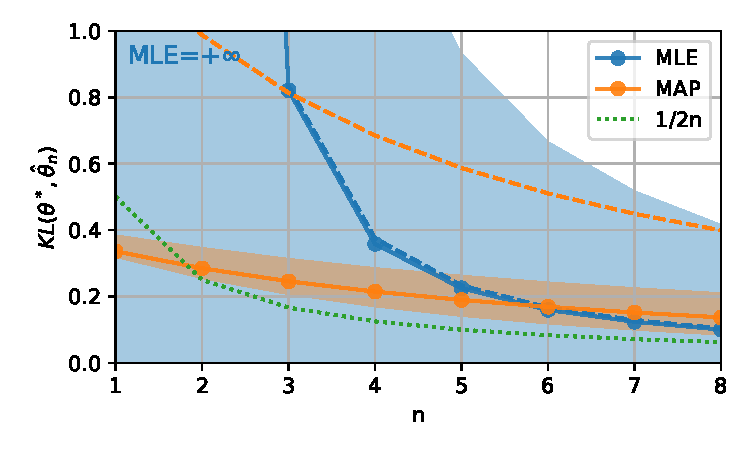
\includegraphics[width=.61\textwidth]{gammaMAPrate.pdf}
	\caption[KL divergence for Gaussian variance MLE and MAP]
	{KL divergence~\eqref{eq:suboptimalityKL} for Gaussian variance (\S\ref{ssec:gaussian-variance}) MLE (blue) and MAP (orange) against number of samples $n$. 
		Solid curve  are average over $10^5$ trials.
		Dashed curves are upper bounds~\eqref{eq:MLE_rate} (blue) and~\eqref{eq:MAP_rate} (orange, not tight by a factor 2).
		Shaded areas are 90\% confidence interval.
		The MLE expected KL is infinite for $n=1$ and $n=2$, but for $n\geq3$ it quickly joins the upper bound~\eqref{eq:MLE_rate} and the $1/2n$ asymptote~\eqref{eq:asymptote}.
		MAP's expected KL is always finite, and it has lower variance than MLE, but it is slower to join the asymptote.
		We wish to find upper bounds similar to~\eqref{eq:MAP_rate} characterizing the relative importance of the prior and the few sample behavior of MAP for a variety of exponential families.
	}
	\label{fig:curves}
\end{figure}


\section{Introduction}
\label{sec:motivation}

\paragraph{Models}
Exponential families are among the most widely used simple parametric models of data, yet, we will highlight some open problems about them in this paper.
Many standard random variables are exponential families: Gaussians, categorical, gamma, or Dirichlet, for example.
They are flexible enough to model a variety of data sources $X$ and easy to describe with some sufficient statistics $T(X) \in \real^d$.
They are particularly appreciated for their convex log-likelihood
\alignn{
f(\nat) := \E[-\log p_\nat(X)] = \logpart(\nat) - \lin{\E[T(X)] , \nat},
\label{eq:defNLL}
}
where $\logpart$ is the convex log-partition function and \mbox{$\nat\in\Theta$} is the \textit{natural parameter}.
This convexity lays the foundation for generalized linear models \citep{mccullagh1989generalized} or variants of principal component analysis \citep{collins2001generalization}, among other applications.

\paragraph{Estimators}
In this paper, we consider the problem of estimating $\nat$ from a dataset $\mD = (X_1, \dots, X_n)$ of iid observations from $p_\theta$ in an exponential family.
In this case, not only is $f$ convex, but it yields a simple condition for the maximum-likelihood estimate (MLE)
\begin{align}
 \hat \mu_n^\text{MLE} = \nabla  \logpart(\hat \nat_n^\text{MLE}) = \frac{\sum_{i=1}^n T(x_i)}{n} \; .
	\label{eq:defMLE}
\end{align}
This rule is also known as moment matching.
Given a specific conjugate prior, a similar formula~\eqref{eq:defMAP} holds for the maximum a posteriori (MAP). In this paper, we will focus on analyzing MLE and MAP estimators.\footnote{A related analysis is present in the online-learning literature, but for different online estimators, which are less efficient than offline methods \citep{azoury2001relative,dasgupta2007online}.}

\paragraph{Statistical decision theory}
To assess the quality of an estimator $\hat \nat$ (and compare them), we need to define some notion of closeness to the correct parameter $\nat^*$.
We distinguish here two ways: \textit{distance in parameter space} and \textit{``distance'' between distributions}.
{\bf 1)} Distance in parameter space $d(\nat,\nat^*)$. This is the focus of \emph{parameter estimation}, yielding results such as the asymptotic efficiency of the MLE via the Cramer-Rao lower-bound \citep{aitken1942estimation} and a wealth of asymptotic results \citep{vdv1998asymptotic}.
In particular for sum of independent variables such as~\eqref{eq:defMLE}, large deviations theory \citep{varadhan1984large} characterizes concentration phenomena.
{\bf 2)} Distance between distributions, as studied in \emph{density estimation}.
For this purpose, the Kullback-Leibler (KL) divergence $\KL\paren{p_{\nat^*} || p_{\nat} }$  arises naturally from information theory,
but its lack of robustness to misspecification\footnote{
For $p$ and $q$ continuous densities,
$\KL(p||q) = +\infty$ if $\exists x, q(x)=0 \, \& \, p(x)>0$.
%Since exponential families have a positive density over their whole input set, this is not a concern for us, except if we misspecified the input set.
}
has led statisticians to study better-behaved distances, such as the $L^2$ norm \citep[\S1.2]{tsybakov2009introduction}, the $L^1$ norm \citep{devroye2001combinatorial}, 
or more recently  $\chi^2$ distance \citep{kamath2015learning} or Hellinger distance \citep{baraud2017new}.
With exponential families, the KL divergence is also a Bregman divergence between parameters (see \S\ref{sec:problem}), thus drawing a connection between these two lines of research,
and raising the fundamental problem:
\begin{equation}
\boxed{
\begin{aligned}
	\textit{Find an upper}&\textit{ bound on the expected value of } \\
	&\KL(p_{\nat^*} || p_{\hat \nat_n^\text{MLE/MAP} }) \; .
\end{aligned}
}
\tag{$\star$}
\label{problem}
\end{equation}

There are already general asymptotic results (\S\ref{ssec:asymptote} and Fig.~\ref{fig:curves}), and a finite $n$ result when $\logpart$ is quadratic (e.g., $X$ is Gaussian with known variance)
or close to quadratic (\S\ref{ssec:quadratic}).
However, a  general solution for finite $n$ remains elusive. 
In this paper, we review partial solutions and give ideas on how to solve the problem.

\paragraph{Optimization} 
Stochastic optimization offers an interesting perspective on~\eqref{problem}.
Consider the problem
\alignn{
	\min_{\theta\in \Theta} f(\theta)\,,
	\label{eq:optimization_problem}
}
solved by $\nat^*\in \Theta$.
Setting $f$ as the log-likelihood~\eqref{eq:defNLL}, the suboptimality is equal to the KL:
\alignn{
	f(\nat) - f(\nat^*) = \KL\paren{p_{\nat^*} || p_{\nat} } .
	\label{eq:suboptimalityKL}
}
Both MLE and MAP can be seen as stochastic algorithms solving~\eqref{eq:optimization_problem}.
In particular, with exponential families, MAP is equivalent to stochastic mirror descent (SMD) \citep{nemirovski2009robust}.
Inspired by recent work~\citep{lepriol2021analysis, kunstner2020homeomorphic}, we consider using existing convergence rates for SMD to get the upper bound we seek.
Unfortunately, none of the current analyses apply, highlighting open problems for the analysis of SMD.

\paragraph{Expected Outcomes}
A solution to~\eqref{problem} can clarify the importance of the prior in MAP, in particular in the few sample regime. %, for instance for Gaussians $\cN(m,\sigma^2)$.
Also, it could enable stochastic optimization to tackle a broad class of barrier objectives.\footnote{we call \emph{barrier} an objective $f$ that is infinite on the boundaries of its domain (assuming they exist).}
A good example is the generalized linear model based on Gaussians with unknown mean and variance, for which there is currently no theory \citep{bach2013nonstronglyconvex}.
It could also help assess the impact of alternative forms of regularization (prior) for these models.

\paragraph{Contributions}
After formalizing the problem~\eqref{problem} (\S\ref{sec:problem}), along with its asymptotic properties (\S\ref{ssec:asymptote}), we make the following contributions.
\begin{itemize}
	\itemsep0em
	\item We provide an upper bound on the KL in the particular case of a Gaussian with known mean but unknown variance $\cN(0,\sigma^2)$ (\S\ref{ssec:gaussian-variance}), illustrating that tight rates are possible even though the current theory does not cover them.
	\item We highlight sufficient conditions to characterize when a (local) quadratic approximation of the KL is valid, offering a partial answer to~\eqref{problem} (\S\ref{ssec:quadratic}-\ref{ssec:local-quadratic}).
	%SLJ REMOVED per Slack discussion
	%\item We leverage a generalized bias-variance decomposition of Bregman divergences\citep{pfau2013generalized}  to formulate a conjecture about~\eqref{problem}(\S\ref{ssec:bias-variance}).
	\item By linking MAP and SMD, we show that modern analysis of SMD is yet to prove convergence on barrier objectives such as $-\log$ (\S\ref{sec:optimization}).
\end{itemize}


\paragraph{Notation}
$X$ and $T=T(X)$ are random variables, $x$ is a sample, $n$ is the number of samples and $d= \dim(T)$.
$\langle \cdot , \cdot \rangle$ is the Euclidean scalar product in $\real^d$.


\section{Technical Background}
\label{sec:background}
This section reviews the formalism of exponential families, their duality, a conjugate prior, and the corresponding MAP.
We point the reader towards \citet[Chapter 3]{wainwright2008graphical} for a more detailed introduction.


The density of an exponential family for a sample $x$ is
\begin{equation}
	 p_\nat(x) = p(x|\nat) = \exp( \langle \nat, T(x) \rangle - \logpart(\nat)) \; ,
	 \label{eq:def_expfamily}
\end{equation}
where  $\nat$ is called natural (or primal) parameter.
It is fully specified by 1) $T: \cX \rightarrow \real^d$, the sufficient statistic,
and 2) a base measure $\nu$ on $\cX$.
Since the exponential is positive, $p$ has the same support as $\nu$.
The log-partition function $\logpart$ acts as a normalization term, since
\begin{align}
    \logpart(\nat) = \log \int e^{\langle \nat, T(x) \rangle} \nu(dx) \;.
\end{align}
This simple model encompasses both categorical distributions : $\cX = \{1, \dots, k\}$, $\nu$ uniform and $T(X)$  the one-hot encoding and multivariate normal distributions $\cX=\real^d, \nu$ Lebesgue and $T(X)=(X, X X^\top)$.

For convenience, we focus on steep, regular exponential families with minimal statistic $T$ \citep{barndoffnielsen2014information}.
Then $\logpart$ is a strictly convex function of Legendre type,
and the set $\Theta = \{ \nat \cond \logpart(\nat) < \infty\}$ is open and convex.
When explicit, we write the random variable $T = T(X)$.

% TODO sort out relationships between : steep family, minimal statistics and Legendre type. What implies what ?

{\bf Duality.}
The log-partition function $\logpart$ verifies the two following identities:
\begin{align}
    \nabla\logpart(\nat) &=  \expect[p_\nat]{T(X)} =: \meanp, \label{eq:mirror-map} \\
    \nabla^2 \logpart(\nat) &= \Cov_{p_\nat}[T(X)] > 0,
\end{align}
where $\meanp$ is called the mean (or dual) parameter, which lives in the open convex set $\cM$ equal to the relative interior of the convex hull of $T(\cX)$.
Given that $\logpart$ is strictly convex, its Hessian is positive definite, and its gradient $\nabla \logpart$ is a \textit{bijection} between natural parameters $\nat$ and mean parameters $\m$.
We will write $\m$ or $\nat$ interchangeably depending on the context, being aware that both are linked and represent the same distribution.

We now introduce the convex conjugate (the Fenchel-Legendre transform) of the log-partition function
\aligns{
	\conj(\m) =  \langle \m, \nat \rangle - \logpart(\nat)
	=  \max_{\nat'\in\Theta}  \langle \m, \nat' \rangle - \logpart(\nat')\; ,
}
which is the common notion of \textit{entropy} in information theory.
By Fenchel duality, its gradient is the inverse of the gradient of $\logpart$,  $\nabla\conj=\nabla\logpart^{-1}$, giving
\aligns{
	\nabla\conj \circ \nabla\logpart(\nat) = \nat, \quad \nabla\logpart\circ \nabla\conj(\meanp) = \meanp.
}
{\bf The Bregman Divergence} induced by $\logpart$ measures the discrepancy between two parameters $\nat$ and $\nat_0$,
\begin{align}
    \bregman (\nat ; \nat_0)
    & = \logpart(\nat) - \logpart(\nat_0)
    - \langle \nabla \logpart(\nat_0)  , \nat - \nat_0 \rangle,
    \label{eq:defBregman}
\end{align}
with $\nabla \logpart(\nat_0) = \expect[\nat_0]{T(X)} =: \meanp_0$ the mean parameter associated to $\nat_0$.
In general, Bregman divergences are not symmetric, i.e., $\bregman (\nat ; \nat_0)\neq \bregman (\nat_0 ; \nat)$.
%Finally, it is equal to the divergence of its convex conjugate with switched arguments,
%\begin{align}
%	\bregman (\nat ; \nat_0)
%    = \bregmanconj ( \meanp_0 ; \meanp) \; .
%    \label{eq:bregman_switch}
%\end{align}

{\bf A Conjugate Prior} for $p(X|\nat)$ is
\begin{align}
    p(\nat)
    &\propto \exp( - n_0 \bregman(\nat ; \nat_0) ) \nonumber \\
    &\propto \exp(n_0 \langle \m_0, \nat \rangle - n_0 \logpart(\nat)),
    \label{eq:def_prior}
\end{align}
where $n_0$ and $\nat_0$ are (hyper)parameters of the prior  \citep{agarwal2010geometric}.
This is an exponential family with sufficient statistics $(\nat ,\logpart(\nat))$ and natural parameter $(n_0 \m_0, -n_0)$.
Intuitively, $n_0$ is the number of fictive data points observed from a distribution with natural parameter $\nat_0$.

{\bf Maximum A Posteriori (MAP).}
Given a dataset $\mD_n =(X_1,\dots,X_n)$, we wish to estimate the maximum of the posterior distribution $p(\nat \cond \mD_n) \propto p(\mD_n|\nat)p(\nat)$.
Plugging in~\eqref{eq:def_expfamily},~\eqref{eq:defBregman} and~\eqref{eq:def_prior} yields
\aligns{
	p(\nat \cond \mD_n)
    \propto \exp(- (n_0+n) \bregman(\nat; \MAPt^\text{MAP}))
%    \label{eq:joint_likelihood}
}
which reaches its maximum at $\MAPt^\text{MAP}$ such that
\begin{align}
    \nabla \logpart(\MAPt^\text{MAP}) = \MAPm^\text{MAP}
    = \frac{n_0 \meanp_0 + \sum_{i=1}^n T_i}{n_0+n} \; ,
    \label{eq:defMAP}
\end{align}
where $T_i=T(X_i)$.
When $n_0=0$ (no samples from the prior), we recover the MLE~\eqref{eq:defMLE}.
We write $\MAPt$ for the MAP and view the MLE as a particular case.


\section{Problems Formulation}
\label{sec:problem}
% Assume we observe a dataset $\mD$ drawn i.i.d. from a distribution $\cD$.
% We further assume that our model is well-specified and there exist $\nat^*\in\Theta$ such that $\cD = p(\cdot \cond \nat)$.
% As we will see, this is already an interesting setting.
% We wish to estimate how well the MLE or a MAP model the true distribution.

We are now ready to formalize the main problem of this paper. Assume we observe a dataset $\mD_n$ drawn i.i.d. from $p(\cdot \cond\nat^*)$, an exponential family distribution
with parameters $\nat^*$.
We wish to quantify how well the MLE or a MAP approximates the true distribution.

A natural way to quantify this is the Kullback-Leibler divergence (KL) $\KL(p_{\nat^*} || p_\nat)$. % should we define it ?
In the well-specified setting, it corresponds to the log-likelihood sub-optimality~\eqref{eq:suboptimalityKL}.
With exponential families, the KL is also a Bregman divergence:
\alignn{
	\KL(p_{\nat^*} || p_\nat)
	 = \bregman(\nat ; \nat^*)
	 = \bregmanconj(\m^* ; \m) \; .
}
The second equality is a general property of Bregman divergences and convex conjugates. % (Be careful about the order of arguments.)
How does this quantity behave when $\hat \nat$ is the MLE or MAP?
 Or in the words of statistical decision theory, what is the \emph{frequentist risk} of these estimators when the loss is the KL divergence?
This is our first problem.

\begin{problem}[Upper-bounding MAP and MLE]
Upper bound the following quantities:
\begin{align}
	\label{eq:bregmanMLE}
	\text{MLE: } \quad &\expect[\mD_n]{\bregmanconj \left (\E_{\nat^*} [T] ;  \inv{n}  \smallsum_i T_i \right )}, \\
	\label{eq:bregmanMAP}
	\text{MAP: } \quad &\expect[\mD_n]{\bregmanconj \left (\E_{\nat^*} [T] ; \frac{n_0 \m_0 + \smallsum_i T_i}{n_0+n} \right )},
\end{align}
where the expectation is on the data $\mD_n = (T_1, \dots, T_n)$.
\end{problem}

More explicitly, we want an upper bound that does not involve this expectation over the dataset.
Surprisingly, we found no general solution to this seemingly simple problem, whether in the literature or by our means.
In \S\ref{sec:example}, we provide results for special cases such as $\cN(0, \sigma^2)$,
while in \S,\ref{sec:insights} we provide realistic conditions to obtain valid bounds after seeing a large number of samples.
However, we have yet to find a solution encompassing both a broad range of exponential families
and applicable to small sample sizes $n \lesssim d$.

{\bf A Difficulty with the MLE.}
While~\eqref{eq:bregmanMAP} is always finite, \eqref{eq:bregmanMLE} may be infinite,
for instance when estimating the covariance of a Gaussian when $n \leq d + 1$.
Even worse, there is a non-zero probability never to sample one of the categories with categorical variables.
In those cases the MLE gives zero weight to this category and $\KL(p_{\nat^*} \,\Vert\, p_\text{MLE} ) = +\infty$.
Therefore, the expected KL~\eqref{eq:bregmanMLE} is infinite for any number of samples.
Instead of taking the expectation, one might want to bound the risk in high probability
without resorting to Markov inequality, as achieved by~\citep{ostrovskii2021finite},
 but this is a difficult endeavor.
These examples make a case for regularized estimators such as MAP,
for which we may find upper bounds.

\paragraph{Optimization.}
With exponential families, MAP can be linked to \emph{stochastic mirror descent (SMD)}, see App.~\ref{app:SMD}.
More precisely, let us re-write~\eqref{eq:defMAP} as
\alignn{
\m_n = \m_{n-1}- \stepsize_n (\m_{n-1} - T_n)
\label{eq:mean_update}
}
where $\stepsize_n := \inv{n_0 + n}$.
Now define stochastic functions $f_X(\nat) = -\log p(X \cond \nat)$ such that $\E[f_X] = f$.
If we further introduce stochastic gradients $g_n(\nat) := \nabla\logpart(\nat) - T_n = \nabla f_{X_n}(\nat)$, then~\eqref{eq:mean_update} becomes
\alignn{
	\nabla\conj(\hat \nat_{n})
	= \nabla\conj(\hat \nat_{n-1}) - \stepsize_n g_n(\hat \nat_{n-1}),
}
which is the update formula for SMD on $f$ with mirror map $\nabla\logpart$
and step-size schedule $\stepsize_n$, initialized at $\nat_0$.
In this view, MLE forgets its (arbitrary) initialization after the first step with step size 1.
The observation MAP $\in$ SMD brings us to our second problem.
\begin{problem}[Convergence rate for SMD]
Find a convergence rate for stochastic mirror descent that applies to conjugate MAP of exponential families such as Gaussians $\cN(\meanp, \sigma^2)$.
\end{problem}

To address these problems, we start by investigating simple examples to provide solutions to Problem 1, getting insights into what is achievable.

\section{Illustrating Examples}\label{sec:example}
\subsection{Gaussian with Unknown Variance}\label{ssec:gaussian-variance}

A non-trivial yet straightforward example is the centered Gaussian distribution with unknown variance $\cN(0,\sigma^2)$.
Its log-likelihood reads $\log p(x) = -\frac{x^2}{2 \sigma^2} - \half\log(2\pi \sigma^2)$.
Defining $T(X)=X^2$ as the sufficient statistic, we get natural parameter $\nat = -\inv{2 \sigma^2} <0$, and mean parameter $\m=\E[T(X)] = \sigma^2 >0$.
Mean and natural parameters are roughly inverse of each other, i.e., $\nat = -\inv{2 \m}$.
Now we match the log-likelihood with the exponential family template to get the log-partition function, and take the conjugate to find the entropy
\aligns{
	\logpart (\nat) = - \half \log(-\nat) \quad\text{and}\quad
	\conj(\m) = - \half \log(\m)  \; ,
}
up to constants.
Both $A$ and  the entropy are roughly negative logarithm $z\mapsto - \log(z)$.
It means the conjugate prior is the exponential family with sufficient statistic $(\nat, \log(-\nat) )$, e.g., a negative gamma distribution.
It also means $\bregman$ and $\bregmanconj$ have the same shape
\begin{align}
	\bregmanconj( \m^*; \m_n)
	&= \half \left ( \frac{\m^*}{ \m_n} - 1 - \log  \frac{\m^*}{ \m_n} \right) \; .
%	\bregman( \nat_n; \nat_* )
%	&=  \half \left ( \frac{ \nat_n}{\nat_*} - 1 - \log  \frac{ \nat_n}{\nat_*} \right) \; .
\end{align}
In Theorems~\ref{thm:varianceMLE} and~\ref{thm:varianceMAP}, we report upper bounds on the expected value of this divergence for the MLE and the MAP.
All proofs for this section are in App.~\ref{app:gaussian-variance}.
\begin{theorem}[MLE Bound]
\label{thm:varianceMLE}
	The MLE of $\cN(0,\m^*)$ is $\hat \m_n^\text{MLE} = \inv{n} \sum_i X_i^2 $.
	Its expected suboptimality is infinite when $n\leq 2$, and otherwise upper-bounded as
	\begin{align}
		 \expect{\bregmanconj( \m^*; \hat \m_n^\text{MLE}) }
			\leq \inv{2n} +\frac{2}{n(n-2)} \; .
			\label{eq:MLE_rate}
	\end{align}
\end{theorem}
This upper bound matches the asymptotic result~\eqref{eq:asymptote} that we derive in \S\ref{ssec:asymptote}.
We illustrate its numerical behavior in Figure~\ref{fig:curves}.
With the same technique, we obtain a similar bound for the multivariate generalization: the expected value is infinite whenever $n \leq d+1$ where $d$ is the dimension, and is otherwise bounded by $O\paren{\frac{d^2}{n} + \frac{d^3}{n(n-d-1)}}$.

\begin{theorem}[MAP Bound]
\label{thm:varianceMAP}
The expected suboptimality of the MAP of $\cN(0,\m^*)$ with prior hyper-parameters $(n_0,\m_0)$ is
 \begin{align}
	& \expect{\bregmanconj( \m^*; \hat \m_n^\mathrm{MAP})}
	\leq \begin{cases}
		\inv{2(n_0+1)}  +  b_1 \ \text{if}\ n=1,\\
		\frac{1}{n_0 \frac{\m_0}{\m^*} +n-2} + b_n \ \text{if}\ n\geq 2
	\end{cases}
	\label{eq:MAP_rate}\\
	& \text{where }b_n = \frac{(1 + \inv{n_0} - \frac{\m_0}{\m^*})^2}{2 (\frac{\m_0}{\m^*}+\frac{\max(0,n-2)}{n_0})(1 + \frac{n}{n_0} )} \; . \nonumber
\end{align}
\end{theorem}
Anticipating on \S\ref{ssec:bias-variance}, this inequality highlights an explicit $O(\frac{v}{n} + \frac{b}{n^2})$ variance-bias decomposition.
This inequality is derived with the symmetrized Bregman $\cB(a,b) + \cB(b,a)$ for which calculus is more tractable.
This explains why the variance term is twice larger than the asymptote~\eqref{eq:asymptote}.
Regarding the bias, it vanishes when $\frac{\m_0}{\m^*} =1 + \inv{n_0} $, which happens when the prior is slightly larger than the ground truth.
This correlates well with our numerical observations (cf App.~\ref{app:gaussian-variance}).

Note that if $X\sim \cN(0,\sigma^2)$, then $X^2 \sim \Gamma\paren{\half, \inv{2\sigma^2}}$ in the shape-rate parametrization of Gamma distributions. In fact the bounds above can be generalized to any distribution $\Gamma\paren{\alpha, \beta}$ with known shape $\alpha$.
This generalization encompasses exponential distribution when $\alpha=1$, as another important special case.
 We postpone these rates to \cref{app:gaussian-variance} for the sake of clarity.

\begin{figure*}[t]
	\centering
	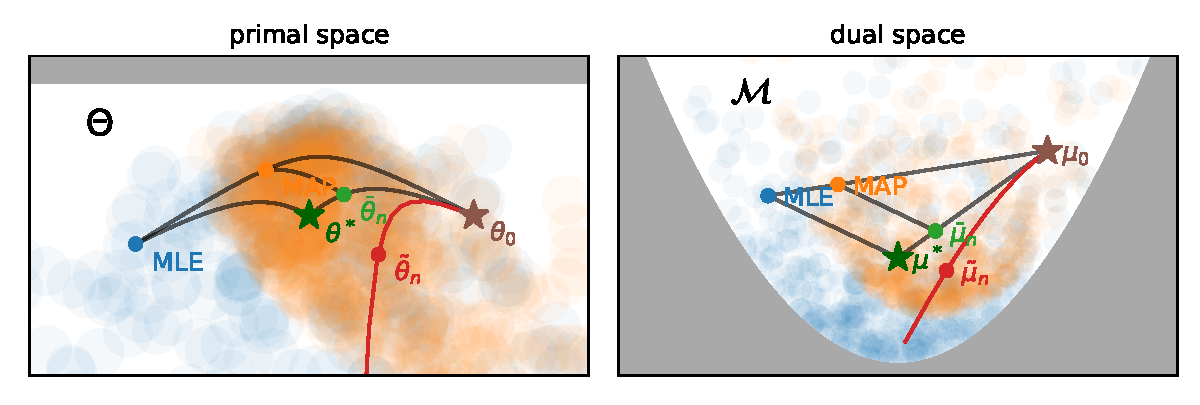
\includegraphics[width=\textwidth]{2d/thales_n=3.pdf}
	\caption[Primal and dual representations of a Gaussian MLE and MAP.]
	{
	Primal and dual representations of a Gaussian $\cN(m,\sigma^2)$ MLE (blue) and MAP (orange) (\S\ref{ssec:gaussian} with $n=3$).
	In dual space, MAP is a scaled version of the MLE~\eqref{eq:defMAP} with expectation $\E[\hat\m_n^\text{MAP}]=:\bar \m_n$ (light green), and MLE is unbiased $\E[\hat\m_n^\text{MLE}]=\m^*$, as illustrated by the parallels in the grey triangle.
	In primal space, MAP has expectation $\tilde \nat_n$ (red), which intervenes in the bias-variance decomposition~\eqref{eq:bias-variance} from~\S\ref{ssec:bias-variance}.
	The hyperparameter of the prior $\nat_0$ controls the brown point's location while varying $n_0$ spans the long edges of the triangle and the red curve.
	Large blurry circles in the background are other instances of MAP and MLE revealing their distribution.
	}
	\label{fig:thales}
\end{figure*}

\subsection{Full Gaussian (Non-Trivial)}
\label{ssec:gaussian}
Now that we have solved the case of $\cN(0,\sigma^2)$, consider the full Gaussian $\cN(m,\sigma^2)$, which offers a highly non-trivial example for Problem 1.
Their log-likelihood reads $p(x) = -\frac{(x-m)^2}{2 \sigma^2} - \half \log(2\pi\sigma^2)$.
With sufficient statistic $T(x)=(x, x^2)$,
the mean parameters are $\m = \E[T(X)] = (m , m^2 + \sigma^2)$ belonging to the open set $\cM= \{(u,v) \cond u^2 < v\}$,
and the natural parameters are $\nat= (\frac{m}{\sigma^2} , \frac{-1}{2\sigma^2}) \in \Theta = \real \times \real_-$.
Examples of MAP and MLE  are represented in \cref{fig:thales} within $\cM$ and $\Theta$ delimited in grey.
Given these parameters, log-partition and entropy are, up to constants,
\alignn{
	\textstyle \logpart(\nat) &= \textstyle \frac{\nat_1^2}{-4\nat_2} - \half \log(-\nat_2) \\ 
	\textstyle \conj(\m) &= \textstyle - \half \log (\mu_2 - \mu_1^2)
}

These functions are neither smooth, nor strongly convex, but they are self-concordant, since $\conj$ is  the logarithmic barrier of a quadratic domain
\citep[p.177, example 4.1.1.4]{nesterov2003introductory}, and self-concordance is preserved by convex-conjugacy~\citep{nesterov1994interior} -- see more details in App.~\ref{app:gaussian}.
We now discuss the general problem and some ways to solve it via direct expansions of the Bregman divergence.

\section{Partial Solutions}
\label{sec:insights}

\subsection{Asymptotic Rate}
\label{ssec:asymptote}
As a reference point for any finite convergence rate, it is interesting to briefly review the classical asymptotic behavior of these quantities as $n \rightarrow +\infty$.
Proofs are in App.~\ref{app:asymptote}, and \citet[\S1.1]{ostrovskii2021finite} offers a more comprehensive review.

Statistics typically give results on $\nat$, but the MAP~\eqref{eq:defMAP} is more simply expressed with $\meanp$, so let us focus on $\bregmanconj$.
Bregman divergences are locally quadratic, as seen via a second order Taylor expansion
\alignn{
    \textstyle \bregmanconj(\m^* ; \m)
    &\textstyle = \frac{1}{2}\norm{\m^* - \m}^2_{\mF}
    + O(\norm{\m - \m^*}^3),
    \label{eq:bregmanTaylor}
}
where the Mahalanobis norm  $\| x \|_{\mF}^2 = x^\top \mF x$  is induced by $\mF  := \nabla^2\conj(\m^*)$, the Hessian of the entropy at the optimum. It happens that  $\mF$ is also the inverse \textit{Fisher information matrix} at $\nat^*$, since
\aligns{
    \mF
    :=\nabla^2\conj(\m^*)
    = \nabla^2\logpart(\nat^*)^{-1}
    = \Cov_{\nat^*}[T(X)]^{-1}  \; .
}
Plugging the MLE~\eqref{eq:defMLE} or MAP~\eqref{eq:defMAP} into~\eqref{eq:bregmanTaylor}, we get
\begin{align}
	\label{eq:asymptote}
	\E \bregmanconj \left (\E [T(X)] ; \hat \meanp_n^\text{MLE/MAP} \right )
	= \frac{d}{2n} + O(n^{- \frac{3}{2}}) \; .
\end{align}
Both MLE and MAP have the same asymptote, as the contribution of the prior $n_0 \meanp_0$ gets negligible for large $n$.
This asymptote is independent of the optimum $\meanp^*$ or $\mF$ for well-specified models.
Actually, $\frac{d}{2n}$ is also the minimax of the KL over all estimators, at least for categorical data \citep{braess2004bernstein, kamath2015learning}.
Next, we focus on the quadratic example,  whose finite sample rate matches~\eqref{eq:asymptote}.

\subsection{Quadratic Case}
\label{ssec:quadratic}
As another classical reference point, we consider the case $\logpart(\nat) = \half \norm{\nat}_2^2$.
For instance, this is the log-partition of a Gaussian with known variance $I$,
\[
	\cX=\real^d,\quad \nu(dx) = \exp\paren{\textstyle \half[-\|x\|^2]} dx,\quad T(x)=x.
\]
In this case, $\conj(\meanp) = \half \norm{\meanp}_2^2$ as well, and both Bregman divergences are squared $\ell^2$ distances since
\begin{align}
	\bregmanconj(\meanp^* ; \meanp) = \half \norm{\meanp^* -  \meanp }_2^2  \; .
\end{align}
Thanks to the independence of samples, we can break down the MLE into individual point's contributions:
\begin{align}
	\expect{\half \norm{\m^* -  \inv{n}  \smallsum_i T_i}_2^2}
	=\frac{\Var(T)}{2n}
	=\frac{d}{2n}.
\end{align}
Adding a reference mean $\m_0$ to get the MAP yields
\begin{align}
		\expect{\half \norm{\m^* -   \MAPm^\text{MAP}}_2^2} \!
	&= \frac{n \Var(T) +  n_0^2 \norm{\m^* -  \m_0}^2}{2(n+n_0)^2} \; .
	%\\ &= O\left(\frac{\Var(T)}{n} \right) + O\left(\frac{\norm{\m^* -  \m_0}^2}{n^2} \right)
	\label{eq:MAP_quadratic}
\end{align}
We see here a variance term defining the $\frac{d}{2n}$ asymptote and a bias term in $O(n^{-2})$. However, this result does not generalize well to other families unless we make restrictive assumptions on $\conj$. % we can relate $\bregmanconj$ to a norm or a quadratic.
% Can we generalize these results to other families?

{\bf If $\conj$ is $L$-Lipschitz} (e.g. $\logpart$ is defined within the $\ell^2$-ball of radius $L$), then
\begin{align}
    \bregmanconj(\m^* ; \m)
    &\leq L \norm{\m^* - \m} + \norm{\nat} \norm{\m^* - \m} \\
    &\leq 2L \norm{\m^* - \m} \; ,
\end{align}
so $\bregmanconj$ is Lipschitz, and~\eqref{eq:MAP_quadratic} yields a $O(\inv{\sqrt{n}})$ rate, but no common exponential families verify the assumption.

{\bf If $\conj$ is $L$-smooth}\footnote{$\conj$ is $L$-smooth iff $\nabla\conj$ is $L$-Lipschitz.} (e.g. $\logpart$ is $\frac{1}{L}$-strongly convex \citep{kakade2009duality}), then
\begin{align}
    \bregmanconj(\m^* ; \m)
    \leq \frac{L}{2} \norm{\m^* - \m}^2 \; ,
\end{align}
so $\bregmanconj$ is upper bounded by a quadratic, and we get~\eqref{eq:MAP_quadratic} as an upper bound.
It is also possible to get (more complex) upper bounds under restricted notions of strong-convexity \citep{negahban2012unified}.
Besides the Gaussian with known variance, the problem is that no standard exponential family has a \textit{globally} strongly convex log-partition function. The next section focuses on \textit{local} quadratic behavior, which is more realistic.

\subsection{Locally Quadratic Case}
\label{ssec:local-quadratic}
From the Taylor expansion~\eqref{eq:bregmanTaylor},
we know that all Bregman divergences are locally quadratic.
Under some assumptions, such as self-concordance\footnote{
In 1d, $f$ is self-concordant iff $\forall x, \abs{f'''(x)} \leq 2 \abs{f''(x)}^{\frac{3}{2}}$.
} of $\conj$ \citep[Ch.~4.1]{nesterov2003introductory}, we can quantify when this quadratic behavior kicks in. Proofs for this subsection are in App.~\ref{app:self-concordant}.
\begin{proposition}
	\label{prop:selfConcordant}
Let $\conj:\cM\rightarrow \real$ be a self-concordant convex function, $\m, \m^* \in\cM$ and $\mF = \nabla \conj(\m^*)$. Then\footnote{$0.21$ is a value of $x$ such that $x^2 \geq -\frac{x}{1-x} - \log(1 - \frac{x}{1-x})$.}
\aligns{
	\norm{\m^*-\m}_{\mF} < 0.21
	\implies
	\bregmanconj(\m^*; \m) \leq \norm{\m^*-\m}_{\mF}^2.
}
\end{proposition}
To gain insights into how many samples are needed, we can estimate when $\expecti{\norm{\m^*-\m}_{\mF}} < 0.21 $.
For the MLE, the proof of~\eqref{eq:asymptote} from~\eqref{eq:bregmanTaylor} yields $\expecti{\norm{\m^*-\hat \m_n}^2_{\mF}} = \frac{d}{n}$ in general, so a sufficient condition is $n \geq 25 d$.
For MAP, transforming~\eqref{eq:MAP_quadratic}, we get the sufficient condition $n\geq 25d + 5 \norm{\m^* -  \m_0} - n_0$.
This means that on average, we need $25$ times more samples than the dimension to reach the quadratic regime and ensure an upper-bound like~\eqref{eq:MAP_quadratic}.

The entropy $\conj$ is self-concordant for several common families such as Gaussians (\S\ref{ssec:gaussian}), and all families with $\logpart \approx -\log$ such as
exponential distributions,
Laplace with known mean,
Pareto with known minimum value,
or Weibull with known shape $k$.
The entropy is also self-concordant when $T$ lives in a compact \citep{bubeck2015entropic} -- e.g., categorical and Dirichlet distributions.
Precisely, categorical variables illustrate that Proposition~\ref{prop:selfConcordant} does not imply directly a bound on the \emph{expected} Bregman.
The expected KL of the categorical MLE is always infinite, as previously mentioned in \S\ref{sec:problem}.
However, Proposition~\ref{prop:selfConcordant} may be used to prove high-probability, many samples, convergence rates for one dimensional (and possibly multivariate) normal distributions.

This is the spirit of
\citet{ostrovskii2021finite}  which characterizes the number of samples needed to be upper bounded by a quadratic \emph{with high-probability}, for any parametric models with a self-concordant log-likelihood $f$.
\citet{anastasiou2017bounds} obtains a similar flavor of result under other assumptions on the third derivative of $f$.
More closely, in the world of exponential families, \citet{kakade2010learning} prove a result similar to Proposition~\ref{prop:selfConcordant} from a local bound on all higher-order moments of $\logpart$ in $\nat^*$.
However, these results are expressed with quadratics in $\nat$, not $\m$, and they do not directly translate to convergence rates for the MAP, but they might with some more work.

More generally, the present proposition and these related works answer~\eqref{problem} only \emph{partially}, as they all give \textit{large sample} results, that hold when $n\geq N$ for some constant $N$. 
A full solution to~\eqref{problem} would apply to small $n$.
Informed by the properties that we have seen so far, we next investigate a general decomposition of the Bregman that could guide us towards a solution.


\subsection{Bias-Variance Decomposition}
\label{ssec:bias-variance}
In both the quadratic~\eqref{eq:MAP_quadratic} and the Gaussian variance examples~\eqref{eq:MAP_rate}, the upper bound takes the form $O(\inv{n}) + O(\frac{\text{bias}}{n^2})$,
giving us a flavor of what we would like as a general result for exponential families: a finite sample convergence rate, with variance and bias terms that reflect the important constants of the problem.
Such a decomposition exists for any Bregman divergence \citep[Theorem 0.1]{pfau2013generalized}.
\begin{theorem}[Bregman Bias-Variance Decomposition]
	Let $\tilde \theta_n := \expecti{\hat \theta_n}$ be the expectation of the MAP in primal space, and $\tilde \m_n = \nabla \logpart(\tilde \theta_n )$ be its dual representation. The  expected Bregman decomposes into
\begin{equation}
	\expect{\bregmanconj(\m^* ; \hat \m_n)} = {\bregmanconj(\m^* ; \tilde \m_n)}
	+ {\expect{\bregmanconj(\tilde \m_n ; \MAPm)}}
	\label{eq:bias-variance}
\end{equation}
\end{theorem}
We plot this decomposition for $\cN(\mu, \sigma^2)$ in Fig.~\ref{fig:gaussian_decomposition} , and we illustrate the primal mean $\tilde \nat_n$ in  Fig.~\ref{fig:thales}.

\textbf{Remark:} In this decomposition, the primal expectation $\expecti{\hat \theta_n}$ is the reference point.
An estimator will be unbiased if $\tilde \nat_n = \nat^*$.
This is not true for the MLE, which is unbiased w.r.t. the dual parameter $\expecti{\hat \m_n}=\m^*$.

We show in App.~\ref{app:bias-variance} that the bias decreases like ${\bregmanconj(\m^* ; \tilde \m_n)} \leq \frac{2}{n(n-2)}$ for Gaussian variance MLE, and
 ${\bregmanconj(\m^* ; \tilde \m_n)} \leq \frac{ \norm{\m^* - \m_0}^2 }{(1 + \frac{n}{n_0})^2 }$ for a quadratic MAP.
These observations hint towards a general $O(1/n^2)$ upper bound for the bias, while the variance may be less dependent on the initialization $\nat_0$.

\begin{figure}[t]
	\centering
	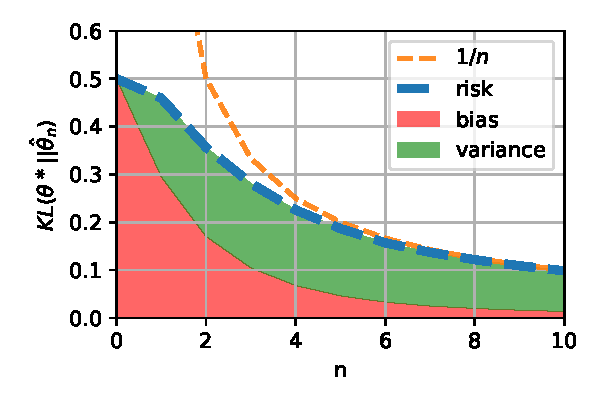
\includegraphics[width=.6\textwidth]{gaussians_bias_variance.pdf}
	\caption[Bias-Variance Decomposition for a Gaussian.]{
	Bias-Variance Decomposition for a Gaussian $\cN(m, \sigma^2)$ with $\meanp^*=(0, 1), \meanp_0 = (1,2)$ and $n_0=1$. The asymptote is $\frac{1}{n}$.
	}
	\label{fig:gaussian_decomposition}
\end{figure}

In this section, we considered direct expansions of~\eqref{eq:bregmanMAP}.
None of them could fully solve~\eqref{problem}.
Next, we investigate whether an optimization approach could solve it.


\section{An Optimization Problem}
\label{sec:optimization}


As we saw in \S\ref{sec:problem}, MAP  can be interpreted as stochastic mirror descent (SMD).
This means that \textbf{1)} we may obtain a convergence rate for MAP from an optimization analysis, and \textbf{2)} any insights gained from MAP may inform other designs and analyses of SMD.
In particular, we know that MAP converges asymptotically as $O(n^{-1})$, so we hope to find a convergence rate for SMD that could capture this behavior. 
We first review the assumptions of relative smoothness, helpful to deal with non-smooth functions, before investigating recent analyses of SMD with the MAP.

\subsection{Relative Smoothness}
Mirror descent (MD) \citep{nemirovski1983problem,beck2003mirror}, also known as
Bregman (proximal) gradient, relative gradient descent or NoLips,
%Nemirovski introduced the algorithm, and Beck established the connection with Bregman divergences, e.g. the argmin form.
and SMD \citep{nemirovski2009robust,ghadimi2012optimal}
are typically encountered in non-smooth (online) optimization,
under bounded (or Lipschitz) gradient assumption on the objective $f$
and strong convexity assumption on the potential $\logpart$
\citep[Th. 4.2(MD) \& Th. 6.3(SMD)]{bubeck2015convex}.
In our case, these assumptions do not hold.
For instance $\logpart = -\log$ is neither smooth nor strongly convex.

Recently, these assumptions have been relaxed to the $\stgcvx$-strong convexity and $\smooth$-smoothness of $f$
\emph{relative} to a reference function $\logpart$, defined as
\aligns{
	\stgcvx \cB_{A}(x ; y)
	\leq
	\cB_f(x ; y)
	\leq
	\smooth \cB_A(x ; y) \; .
}
When $\logpart = \norm{\cdot}^2$, we recover the standard smoothness and gradient descent.
These conditions ensure the linear convergence of MD with mirror map $\nabla A$
\citep{birnbaum2011distributed, bauschke2017descent, lu2018relatively},
even when $f$ is not smooth, and $\logpart$ not strongly convex.

For exponential families, MAP perfectly fits into this framework, as
\aligns{
	f(\theta) = A(\theta) - \expect{\lin{T(X), \theta}}
}
is $1$-smooth and $1$-strongly convex relative to $A$.
Our goal is then to find an applicable convergence rate for SMD under relative smoothness.

\subsection{Bounding the Randomness}

To analyze stochastic algorithms, one also needs to quantify the randomness of stochastic gradients $g(\nat)$.
While many assumptions exist for SGD \citep[\S3 for a modern review]{khaled2020better}, only a few have been adapted to SMD with relative smoothness \citep{hanzely2018fastest, dragomir2021fast, dorazio2021stochastic}, but they have so far been lacking concrete examples.
We review these analyses in the light of the MAP and provide a summary in \cref{tbl:assumptions}.

\begin{table}[t]
	\newcommand*{\greencmark}{\textcolor{Green}{\cmark}}
	\newcommand*{\redxmark}{\textcolor{Red}{\xmark}}
	\caption[Summary of results for SMD]{Summary of results for SMD
		under relative smoothness and relative strong convexity assumptions.
		Each row correspond to one analysis, and each columns answers one question.
		($-\log$) does the bound hold for the Gaussian variance example (\S\ref{ssec:gaussian-variance})?
		($\stepsize_n \sim \inv{n}$) does it converge with a $O(\inv{n})$ step-size?
		($f$) is the bound in function value, or in reverse Bregman $\bregman(\nat^* ; \hat\nat_n)$?
		($\hat\nat_n$) is it for the last iterate or an average ?
		None of these analysis check all the boxes needed to address~\eqref{problem}.
	}
	\begin{center}
		\begin{tabular}{lcccc}
			%{p{.15\textwidth}m{.05\textwidth}m{.08\textwidth}m{.1\textwidth}}
			\toprule
			Boundedness & $-\log$ &  $\stepsize_n \sim \inv{n}$ & $f$ & $\hat\nat_n$ \\
			\midrule
			%Strongly convex and bounded variance\newline
			%\citep[e.g.,][]{??}
			%&
			%$
			%\cB_A(\theta,\theta') \geq \frac{1}{2}\norm{\theta-\theta'}^2,
			%\quad
			%\expect[x]{\norm{\m - x}}^2\leq\sigma^2
			%$
			%\\
			Variance on $\Theta$~\eqref{eq:hanzely} % \newline \citep{hanzely2018fastest}
			& \redxmark & \greencmark & \greencmark  & \redxmark
			\\
			Variance at $\theta^*$~\eqref{eq:dragomir} %\newline \citep{dragomir2021fast}
			& \redxmark & \greencmark & \redxmark  & \greencmark
			\\
			Optimization gap~\eqref{eq:dorazio} %\newline \citep{dorazio2021stochastic}
			& \greencmark & \redxmark & \redxmark & \greencmark
			\\
			\bottomrule
		\end{tabular}
	\end{center}
	\label{tbl:assumptions}
\end{table}


%Before we proceed, let $f_X$ be a stochastic estimate of $f = \expecti{f_X}$, with stochastic gradients $g_X(\nat) =\nabla f_X(\nat)$. In our case $f_X(\nat) = - \log p(X\cond \nat)$ and $g_X(\nat) = \m - T(X)$.

\subsubsection{Analogs of the Variance}
Let us introduce the symmetrized Bregman induced by $\conj$, written $\cS_\conj(\m_1 ; \m_2) = \bregmanconj(\m_1 ; \m_2) + \bregmanconj(\m_2 ; \m_1)$.
\citet{hanzely2018fastest} assume that the expectation of $\cS$ between stochastic and deterministic updates verifies
\alignn{
	\expect[g\!]{\cS_\conj \paren{
			\hat\m_{n} - \stepsize g(\hat \nat_{n}) ;
			\hat\m_{n}   -\stepsize \nabla f(\hat \nat_{n})
	}} \leq \stepsize^2 C
	\label{eq:hanzely}
}
for all possible iterates $\MAPt$, relevant step-sizes $\stepsize$ and for some constant $C$.
When $A(\theta) = \frac{1}{2}\norm{\theta}^2$,
%or when $A$ is $\stgcvx$-strongly convex,
this definition recovers the variance of the stochastic gradient
\alignn{
	\expect[g\!]{\norm{\nabla f(\theta) - g(\theta)}^2}\leq C \; .
	\label{eq:gradient-var}
}
Under this assumption, \citet[Lem.4.8]{hanzely2018fastest} prove a $O(1/n)$ convergence rate on function values with $O(1/n)$ step-sizes and tail averaging \citep{lacostejulien2012simpler} in primal space $\Theta$.

\citet{dragomir2021fast} define the assumption
\alignn{
	\expect[g\!]{
		\cB_{A^*}(\MAPm - 2\stepsize g(\theta_*), \MAPm)
	} \leq 2 \stepsize^2 C \; .
	\label{eq:dragomir}
}
When $A(\theta) = \frac{1}{2}\norm{\theta}^2$,
% or when $\logpart$ is $\stgcvx$-strongly-convex,
we recover the variance of the gradients at the optimum, which is weaker than~\eqref{eq:gradient-var},
\alignn{
	\expect[g\!]{\norm{\nabla g(\theta^*)}^2}\leq C \; .
	\label{eq:opt-gradient-var}
}
%Note that~\eqref{eq:opt-gradient-var} is weaker than~\eqref{eq:gradient-var}.
Using their descent lemma \citep[Eq. (12)]{dragomir2021fast} with the $O(1/n)$ step-size used by \citet[Th. 3.2]{gower2019sgd} for SGD, we obtain a $O(1/n)$ convergence rate, on the Bregman with \emph{reversed} arguments $\bregman(\nat^* ; \hat\nat_n)$.

These two analyses seem promising for~\eqref{problem}, but none of these assumptions hold in front of barrier objectives such as the $-\log$ from \S\ref{ssec:gaussian-variance}.
Indeed, they both assume their bound holds uniformly for every possible iterate $\hat \nat_n$.
Yet $\cN(0,\sigma^2)$ has a positive mass around $0$.
This means that $\hat \m_n$ can get arbitrarily close from $0$, where the $-\log$ is unbounded, along with the associated  Bregman divergences~\eqref{eq:hanzely} and~\eqref{eq:dragomir}.
In general, this uniform bound over $\hat \m_n$ cannot hold for \emph{barrier} objectives -- functions exploding to infinity in some finite point of space.

Both of their proofs hold if we add an expectation over $\MAPm$ to their assumption.
However, this is not helpful, as verifying the assumption becomes as hard as the initial problem.
For instance, the expectation of~\eqref{eq:hanzely} over $\MAPm$ is an upper bound on the variance term of~\eqref{eq:bias-variance} (cf App.~\ref{app:bias-variance}).
Confronted with this difficulty, we investigate an alternative definition of variance.

\subsubsection{Bounded Optimality Gap}
Inspired by \citet{loizou2021stochastic}, \citet{dorazio2021stochastic} explore the hypothesis
\alignn{
	\min_\nat f(\nat) - \expect[X]{\min_\nat f_X(\nat)} \leq C \; ,
	\label{eq:dorazio}
}
where $f_X$ is a stochastic estimate of $f = \expecti{f_X}$. In our case $f_X(\nat) = - \log p(X\cond \nat)$.
In other words, this lower bounds the expectation of the minimum of the stochastic estimates.
For probabilistic models, such a bound is finite as soon as the model cannot give infinite density to any data point $x$.
This holds, for instance, for discrete distributions because the probability mass is upper bounded by $1$; however, it rules out many families.
In the case of normal distributions $\cN(m, \sigma^2)$, setting $m=x$ and $\sigma^2 \rightarrow 0$ gets $p_\nat (x) \rightarrow +\infty$,.
%A similar behavior holds for Gamma, Beta, inverse Gaussians, log-normal, Gamma or inverse Gamma distributions.
We have a similar behavior for gamma distribution with $\alpha = \beta x$ and $\beta \rightarrow +\infty$, or with the beta distribution with $\alpha=\beta \frac{x}{1-x}$ and $\beta \rightarrow +\infty$.
Other counter-examples include inverse Gaussians, log-normal, gamma, inverse gamma.

It is possible to overcome this limitation by treating batches of samples as single samples by averaging sufficient statistics, e.g.,. $Y = \{X_1, \dots, X_k\}$ and $T(Y) = \inv{k}\sum_i T(X_i)$.
For instance, a multivariate normal of dimension $d$ cannot attribute infinite density to $d+1$ samples that are not in an affine subspace.

Overall, \eqref{eq:dorazio} can partially handle barrier objectives, but it fails to account for the step-size $\stepsize_n = \inv{n_0+n}$, as \citet[Thm.1]{dorazio2021stochastic} only proves linear convergence to a variance ball of size $\frac{C}{\stgcvx}$ under constant step-size.
This is in contrast with~\citet{dragomir2021fast} which can handle decreasing step-sizes but not barrier objectives.
Proving convergence of stochastic mirror descent on barrier loss remains an open problem.

\section{Conclusion}
Despite the MLE and MAP estimators in the exponential family being classical and known in statistics for decades, we highlighted in this paper open problems to bound their frequentist risk (the expected KL) in a non-asymptotic way. We reviewed some partial results, such as a large sample analysis that describes how many samples are needed to ensure a locally quadratic regime~\citep{kakade2010learning, ostrovskii2021finite} for which rates are known. We also related this problem to the one of obtaining convergence rates in stochastic optimization, observing that MAP fits the framework of stochastic mirror descent with relative smoothness assumptions.
Nevertheless, none of the current analyses of SMD hold for the MAP, even on a simple family such as $\cN(0,\sigma^2)$, thus revealing an area for progress in non-Euclidean optimization.
In writing this paper, we hope to attract attention to this fundamental problem, leading to progress in both optimization and statistics.


\clearpage

\begin{subappendices}

\section{Proofs for Gaussian Variance}
\label{app:gaussian-variance}


In this section, we prove the results mentioned in \S\ref{ssec:gaussian-variance},
and add some context and experimental observations.
As mentioned in the main text, the centered gaussian $\cN(0,\sigma^2)$ has sufficient statistic $T(X)=X^2$ which follows a gamma distribution $\Gamma\paren{\half, \inv{2 \sigma^2}}$. 

In general, if $X$ is part of the exponential family, then $T(X)$ is part of the natural exponential family with the appropriate support and base measure, with the same log-partition function as $X$ up to constants.
MLE and MAP only depend on $T(X)$, not $X$, so their performance only depends on the distribution of $T(X)$.
 
In this section we derive results for samples  from a general gamma distribution $X \sim \Gamma(\alpha,\beta)$ with known shape parameter $\alpha$, but unknown rate parameter $\beta$.
Results for the Gaussian follow by taking $\alpha=\half$,
We also immediately get results for exponential distributions by taking $\alpha=1$.
For instance for the MLE we derive the following theorem:

\begin{theorem}[MLE Upper Bound]
	\label{thm:gammaMLE}
	Consider an exponential family such that $T(X)$ is a gamma $\Gamma(\alpha, \beta)$ with known shape $\alpha$.
	the expected KL between $\mu_*$ and the MLE $\hat\mu_n$	is infinite when $\alpha n\leq 1$ and otherwise upper bounded by
	\begin{align}
		 \expect{\bregmanconj( \mu_*; \hat \mu_n) }
			\leq \inv{2n} + \frac{1}{n(n \alpha-1)}  \; .
	\end{align}
\end{theorem}
	
To obtain the result for Gaussian variance (see Theorem~\ref{thm:varianceMLE}), it suffices to set $\alpha=\half$ in Theorem~\ref{thm:gammaMLE}.

In this section, we review useful properties of the gamma distribution and associated Bregman divergence in \S\ref{app:gamma}. 
Then we prove theorem~\ref{thm:gammaMLE} in \S\ref{app:gammaMLE}.
Then we prove an extension of theorem~\ref{thm:varianceMLE} in \S\ref{app:multivariateMLE}, and prove a useful lemma about the expectation of the natural parameter of the MAP in \S\ref{app:nat-bound}, in order to prove upper bounds for the MAP in \S\ref{app:MAP-bound}.
Finally we numerically investigate the effect of prior hyper-parameters in \S\ref{app:prior-choice}.

\subsection{Gamma Distribution}
\label{app:gamma}
The density of $\Gamma(\alpha,\beta)$ reads
\alignn{
	p(x) = \frac{\beta^\alpha}{\Gamma(\alpha)} x^{\alpha-1} e^{-\beta x} \; .
}
When $\alpha$ is known, it can be cast as an exponential family~\eqref{eq:def_expfamily} with sufficient statistic $T(x)=x$, domain $\cX = \real_+$ and base measure $\nu(x)\propto x^{\alpha-1}$. Then the natural parameter is $\nat = -\beta < 0$ and the log-partition function is
\alignn{
	\logpart (\nat) = -\alpha \log(-\nat)  + \log\Gamma(\alpha) \; .
}
From there we find that the mean parameter is $\mu = \frac{\alpha}{-\nat} >0$ and the entropy has the same form as the log-partition $\conj(\mu) = - \alpha \log(\mu) + \cst$.
This means that the primal and dual Bregman divergences have the same form as well
\begin{align}
	\bregmanconj(\m_*; \m_n) 
	&= \alpha \left ( \frac{\m_*}{ \m_n} - 1 - \log  \frac{\m_*}{ \m_n} \right) 
	= \alpha \phi\paren{\frac{\m_*}{ \m_n}},
	\\
	\bregman( \nat_n; \nat_* ) 
	&=  \alpha \left ( \frac{ \nat_n}{\nat_*} - 1 - \log  \frac{ \nat_n}{\nat_*} \right)
	= \alpha \phi\paren{\frac{ \nat_n}{\nat_*}},
\end{align}
\begin{wrapfigure}[12]{l}{0.3\textwidth}
	\centering
	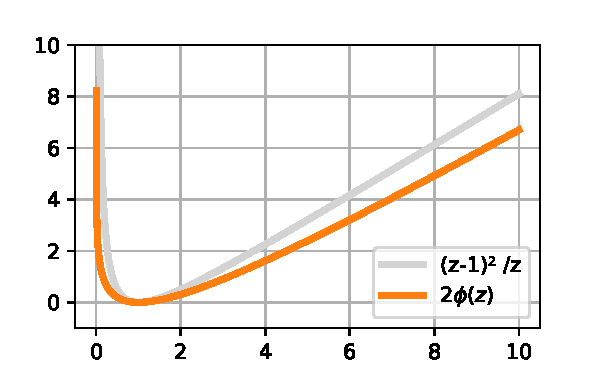
\includegraphics[width=.28\textwidth]{phi.pdf}
	\caption[Illustration of $\phi(z)$ and its upper bound.]{
	Illustration of $\phi(z)$ (orange) and its upper bound $\phi(z) + \phi\paren{z^{-1}}$ (grey).
	They both are barriers near $0$.
	}
	\label{fig:phi}
\end{wrapfigure}
where these 2 lines are equal, and $\phi$ measures the discrepancy between the ratio $\frac{ \nat_n}{\nat_*} =  \frac{\m_*}{ \m_n}  $ and $1$ via the function
\begin{align}
	\phi(z) := z - 1 - \log(z),
\end{align}
illustrated in orange in Figure~\ref{fig:phi}.
To derive the upper bound for the MAP, due to the difficulty of finding a closed form for the expectation of the logarithm, we focus on the symmetrized Bregman instead
\alignn{
	\cS_{\conj} (\mu_*, \mu_n )
	&:= \bregmanconj( \mu_*; \mu_n)  + \bregmanconj( \mu_n; \mu_*) \\
	&= \alpha\phi\paren{\frac{\mu_*}{\mu_n}} + \alpha\phi\paren{\frac{\mu_n}{\mu_*}} \\
		&=  \alpha \paren{\frac{ \mu_*}{\mu_n} -1 +\frac{ \mu_n}{\mu_*} - 1 } \; ,
	\label{eq:symmetrized_bregman}
}

which verifies $\bregmanconj( \mu_*; \mu_n) \leq \cS_{\conj} (\mu_*, \mu_n )$.
Writing $z=\frac{\mu_*}{\mu_n}$ this is equivalent to
\aligns{
	\label{eq:log_bound}
	\phi(z) \leq \phi(z) + \phi\paren{z^{-1}}
	&=  z -1  + \inv{z} -1
	= \frac{(z-1)^2}{z} \; ,
}
which is illustrated by the grey upper bound in Figure~\ref{fig:phi}.



\subsection{Proof for the MLE}
	\label{app:gammaMLE}
	
	\begin{proof}
	Since $T(X)$ follows a gamma distribution $\Gamma(\alpha, \beta)$, the MLE is a scaled sum of gammas $\hat \mu_n = \inv{n} \sum_i T(X_i)$.
	As such it is also a gamma with parameter $\Gamma(n \alpha, n \beta)$ and expectation $\frac{n\alpha}{n\beta} = \frac{\alpha}{\beta} = \mu_*$.
	If we consider the ratio $\frac{\MAPm}{\mu_*}$, it is also a gamma with parameter $\Gamma(n \alpha, n \alpha)$.
	Its inverse follows an inverse gamma distribution with expectation
	\begin{equation}
		\expect{\frac{\mu_*}{\hat \mu_n}} 
		= \begin{cases}
			\frac{n\alpha}{n \alpha -1 }\ \text{ if } n\alpha > 1, \\
			+\infty \  \text{ otherwise. }
		\end{cases}
	\end{equation}
	which implies that for $n\alpha>1$, 
	\begin{align}
		\expect{\frac{\mu_*}{\hat \mu_n}} -1  
		= \frac{n \alpha}{n\alpha -1 } - 1
		= \frac{1}{n \alpha -1}
	\end{align}
	There is also a closed form solution for the expected logarithm of a gamma.
	Indeed, the sufficient statistic of a gamma is $(X, \log(X))$, so one can apply formula~\eqref{eq:mirror-map} on the log-partition of a gamma to get
	\begin{align}
		\expect{\log \frac{\hat \mu_n}{\mu_*}} 
		= \psi\paren{n \alpha} - \log\paren{n \alpha},
	\end{align}
	where $\psi$ is the \href{https://en.wikipedia.org/wiki/Digamma_function}{digamma function.}
	%Closed forms also exist for non-central chi-squares, see for example the note of \citep{pav2015moments}.
	Consequently the suboptimality of the MLE has a closed form solution
	\begin{align}
	\expect{\bregmanconj( \mu_*; \hat \mu_n) }
	&= \alpha \expect{\frac{\mu_*}{ \hat \mu_n} - 1 + \log \left(\frac{\hat \mu_n}{\mu_*} \right) },
	\\
	& =
	\begin{cases}
		\alpha \paren{ \frac{1}{n\alpha - 1} + \psi\paren{n \alpha} - \log\paren{n \alpha} }, \ \text{ if } n\alpha>1, \\
			+\infty \  \text{ otherwise. }
	\end{cases}
	\end{align}
	Surprisingly, for a gaussian variance where $\alpha = \half$, we need $3$ samples or more for the expected loss to be bounded.
	When the expectation is finite, we can get a more interpretable formula using known \href{https://en.wikipedia.org/wiki/Digamma_function#Inequalities}{bounds on the digamma function},
	\begin{align}
		-\inv{x} \leq \psi(x) - \log(x) \leq -\inv{2x} = - \inv{x} + \inv{2x}	\; ,
	\end{align}
	giving, for $n \alpha >1 $,
	\begin{align}
		\frac{\alpha}{n\alpha-1} - \frac{\alpha}{n\alpha}
		&\leq \expect{\bregmanconj( \mu_*; \hat \mu_n) }
		\leq \frac{\alpha}{n\alpha-1} - \frac{\alpha}{n\alpha} + \frac{\alpha}{2n\alpha}
		\\
		\iff
			\frac{1}{n(n \alpha-1)}
			&\leq \expect{\bregmanconj( \mu_*; \hat \mu_n) }
			\leq \inv{2n} + \frac{1}{n(n \alpha-1)} \; ,
	\end{align}
	so we get a $\Omega(n^{-2})$ lower bound and a $O(n^{-1}) + O(n^{-2})$ upper bound.
	\end{proof}


\subsection{Multivariate MLE}
\label{app:multivariateMLE}

For the sake of simplicity, in higher dimension we focus on Gaussian covariance estimation and avoid the general Wishart discussion. 
In higher dimensions, $X \sim \cN(0, \mu_*)$, $X\in\real^d$, $T(X) = XX^\top$, and the mean parameter $\mu_*$ 
is a $d \times d$ symmetric, positive definite covariance matrix with $p = \frac{d(d+1)}{2}$ degrees of freedom.
Note that here $d$ denotes the dimensionality of the data $X$, rather than the dimensionality of the parameters $\mu_*$.

\begin{theorem}[Multivariate MLE Upper Bound]
	The MLE of  the covariance matrix of $X_i\sim\cN(0,\mu_*)$ is $\hat \mu_n = \inv{n} \sum_i X_i X_i^\top \in\real^{d\times d}$ with $p = \frac{d(d+1)}{2} $ degrees of freedom. 
	The expected KL divergence between $\mu_*$ and $\hat\mu_n$ 
	is infinite when $n\leq d+1$ and otherwise upper bounded by
	\alignn{
	 	\expect{\bregmanconj( \mu_*; \hat \mu_n^\text{MLE(d)})}
 	\leq \frac{p}{2n} + \frac{p(d+2)}{n (n - d -1)} 
 	\ , \forall n >d+1 \;.
}
\end{theorem}
We see from~\eqref{eq:asymptote} that this bound is asymptotically tight.
\begin{proof}
The entropy of $X$ is a negative log-determinant $\conj(\mu) = -\log\det(\mu)$, whose gradient is the negative matrix inverse $\nabla\conj (\mu) = - \mu^{-1}$.
The associated Bregman divergence is
\alignn{
	\bregmanconj(\mu_*; \hat \mu_n) 
	= \half \paren{\Tr(\mu_* \hat \mu_n^{-1} ) - d  - \log\det(\mu_* \hat \mu_n^{-1}) } \; .
}
Thanks to the linearity of the trace, the expectation becomes
\alignn{
	\expect{\bregmanconj(\mu_*; \hat \mu_n) }
	= \half \paren{\Tr(\expect{\mu_* \hat \mu_n^{-1}} ) - d   
	+\expect{\log\det( \hat \mu_n \mu_*^{ -1}))} } \; .
}
When the estimator is the MLE, $\hat \mu_n = \inv{n} \sum_i X_i X_i^\top$, 
then we define the mean parameter ``ratio'' as
\aligns{
	\mV &:= n \mu_*^{-\half}\hat \mu_n \mu_*^{-\half} = \sum_i (\mu_*^{-\half} X_i) (\mu_*^{-\half}X_i)^\top,
}
such that $\Tr(\mu_* \hat \mu_n^{-1})  = n \Tr(\mV^{-1})$.
But $\mu_*^{-\half}X_i \sim \cN(0,\mI)$, so that $\mV$
is sampled from a Wishart  $\cW(\mI, n)$, where $\mI$ stands for the identity matrix of order $d$.
Recall that $\E[\mV] = n \mI$.
Thanks to $\log\det$ being a sufficient statistic of the Wishart, and the natural to mean parameter formula~\eqref{eq:mirror-map}, we have a closed form for the expected log-determinant of a Wishart 
\aligns{
	\E[\log\det \mV] &= \psi_d\paren{\half[n]} + d \log 2 \; ,
}
where $\psi_d(\half[n]) = \sum_{i=0}^{d-1} \psi ( \half[n - i])$ is the multivariate digamma function.
The expectation of an inverse Wishart  is straightforward to compute from the density and the log-partition function
\begin{equation}
	\E[\mV^{-1}] = \begin{cases}
		+\infty \text{ if } n\leq d+1 \\
		 \frac{\mI}{n - d - 1} \text{ otherwise,} 
	\end{cases}
\end{equation}
which proves the infinite part of the statement.
Consider now the case $n>d+1$. Using
\alignn{
	\Tr(\expect{\mu_* \hat \mu_n^{-1}}) - d
	= n\Tr(\E[\mV^{-1}]) - d 
	= \frac{nd}{n - d - 1} -d
	= \frac{d (d+1)}{n -d -1}
	= \frac{2p}{n -d -1},
}
and putting it all together, we get the following closed form for the expectation of the divergence
 \begin{align}
 	\label{eq:where-we-put-it-back-together-multivariate-gaussian}
 	\expect{\bregmanconj( \mu_*; \hat \mu_n^\text{MLE(d)})}
 	= \frac{p}{n-d-1} + \half \left ( \psi_d\paren{\half[n]} - d \log\paren{\half[n]}  \right ).
 \end{align}
To bound $\psi_d$, we can use the same bound as in the univariate case, $\psi(x) \leq \log(x) - \inv{2x}$, to get
\begin{align}
	\psi_d\paren{\half[n]} - d \log\paren{\half[n]}
	&= \sum_{i=0}^{d-1} \paren{\psi \paren{\half[n - i]} - \log\paren{\half[n]} } \\
	&\leq \sum_{i=0}^{d-1} \paren{\log\paren{\half[n-i]} - \inv{n-i} - \log\paren{\half[n]} } \\
	&= \sum_{i=0}^{d-1} \paren{\log\paren{1 - \frac{i}{n}} - \frac{1}{n-i}} \; .
	\label{eq:psid_bound}
\end{align}
We can bound sum of reciprocals $\sum_{i=0}^{d-1} \frac{1}{n-i}$ by the typical bound on 
the harmonic sum $H_n = \sum_{k=1}^n \frac{1}{k}$,
\aligns{
	\inv{2n +1}
	\leq H_n - \log(n) - \gamma \leq 
	\inv{2n - 1},
}
where $\gamma$ is the Euler constant. Then
\begin{align}
	- \sum_{i=0}^{d-1} \frac{1}{n-i} 
	= H_{n-d} - H_n
	&\leq \log(n-d) + \gamma + \inv{2(n-d) - 1} - \log(n) - \gamma - \inv{2n+1} \\
	&= \log\paren{1 - \frac{d}{n}}  + \frac{2(d + 1)}{(2n+1)(2(n - d) - 1)} \\
	&< \log\paren{1 - \frac{d}{n}}  + \frac{d + 1}{2n(n - d - 1)} \; .
\end{align}
Plugging this back into~\eqref{eq:psid_bound} yields
\begin{align}
	\psi_d(\half[n]) - d \log(\half[n]) 
	\leq \sum_{i=0}^{\textcolor{red}{d}} \log\paren{1 - \frac{i}{n}}
	+  \frac{d + 1}{2n(n - d - 1)} \; ,
\end{align}
where the sum now goes up to $d$.
To bound the remaining sum, we use $\log(1+x)\leq x$ (for $x > -1$) to get
\begin{align}
	\sum_{i=0}^{d} \log\paren{1 - \frac{i}{n}}
	\leq \sum_{i=0}^{d} - \frac{i}{n}
	 = -\frac{d(d+1)}{2n} = -\frac{p}{n} \; .
\end{align}
Putting those bounds together in 
\cref{eq:where-we-put-it-back-together-multivariate-gaussian}
and reorganizing yields
\begin{align}
 	\expect{\bregmanconj( \mu_*; \hat \mu_n^\text{MLE(d)})}
 	&< p \paren{ \inv{n-d-1} - \inv{2n}}  + \frac{d + 1}{4n(n - d - 1)}\\
 	&= p \frac{n + d +1}{2 n (n-d-1)}  + \frac{d(d + 1)/2}{2dn(n - d - 1)}\\
 	&= p\frac{n-d-1}{2n(n-d-1)} + p\frac{2(d+1)}{2 n (n-d-1)} + \frac{p}{2dn (n - d - 1)}\\
 	&= \frac{p}{2n} + \frac{p(d+ 1 + \inv{2d})}{n (n-d-1)} \\
 	&\leq \frac{p}{2n} + \frac{p(d+2)}{n (n - d -1)}
 	\ , \forall n >d+1 \;.
\end{align}
where $p = \frac{d(d+1)}{2}$ and the last inequality used $\inv{2d}\leq 1$. 
\end{proof}

\subsection{Bounding the Expected Natural Parameter for the MAP}
\label{app:nat-bound}
Before proving a convergence rate for the MAP, we need to bound the expectation of its inverse, hence the following lemma.
We introduce the notation $(z)_+ = \max(0,z)$.
\begin{lemma}[Expected MAP natural parameter]\label{lem:expected-map-natural-parameter-gaussian}
	Define the variable $a = n_0 \frac{\mu_0}{\mu^*}$, which characterizes 
	the importance of the prior relative to the true parameters.
	The expectation of the natural parameter of a MAP of $\Gamma(\alpha,\beta)$ is bounded by
\begin{equation}
		\frac{n_0+n}{a+n}
		=\frac{\mu^*}{\mu_n}
		\leq \expect{\frac{\mu^*}{\MAPm}} 
		= \expect{\frac{\MAPt}{\nat^*}} 
		\leq
		\frac{n_0 +n}{a+(n-\inv{\alpha} )_+} \; , \forall n\geq 0 \; .
		\label{eq:lemma_nat_bound}
	\end{equation}
\end{lemma}

\begin{proof}
	The lower bound can be readily obtained by applying Jensen's inequality 
	to the convex function $x\mapsto\inv{x}$ for $x>0$.
	The upper bound requires more work.
	To start, let us plug in the definition of $\MAPm$
\alignn{
		\expect{\frac{\mu^*}{\MAPm}} 
		= \expect{\frac{\MAPt}{\nat^*}} 
		= \expect{\frac{(n_0+n) \mu^*}{n_0 \mu_0 + \sum_i X_i}}  
		= \expect{\frac{n_0+n}{n_0 \frac{\mu_0}{\mu^*}+ \sum_i \frac{X_i}{ \mu^*} }} 
		= \expect{\frac{n_0+n}{a + \Gamma(n\alpha, \alpha)}} \; ,
}
	where  $\sum_i \frac{X_i^2}{ \mu^*} \sim \Gamma(n\alpha, \alpha)$ is a gamma random variable and $a=n_0 \frac{\mu_0}{\mu^*}$. 
	Further note that 
\alignn{
	\expect{\frac{n_0+n}{a + \Gamma(n\alpha, \alpha)}} 
	= \frac{n_0 + n}{a} \expect{\frac{1}{1 + \Gamma(n \alpha , a \alpha) }} \; .
}
This kind of integrals can be expressed with {generalized exponential integral functions}
	\begin{align}
		E_k(z) = \int_1^\infty \frac{e^{-z t} }{t^k} dt \; ,
	\end{align}
with \href{http://dlmf.nist.gov/8.19.E4}{the formula} \citep[Eq.~8.19.4]{DLMF}
\alignn{
	\expect{\frac{1}{1 + \Gamma(\alpha , \beta) }}
	= \frac{\beta^{\alpha}}{\Gamma(\alpha)} \int_0^\infty \frac{x^{\alpha-1}e^{-\beta x} }{1+x}  dx 
	= \beta e^{\beta} E_\alpha (\beta) \; .
	\label{eq:expect1+gamma}
}
Overall we get
\alignn{
\expect{\frac{\mu^*}{\MAPm}}  = (n_0 +n) \alpha e^{a \alpha} E_{n\alpha} ( a \alpha) 
}
	Now our goal is to bound this generalized exponential integral with simpler functions.
	Fortunately, mathematicians have been working on these integrals for decades.
	For instance , we have \href{https://dlmf.nist.gov/8.19.E21}{the general bound} \citep[Eq.~8.19.21]{DLMF}
	\begin{align}
		e^x E_k(x) 
		&\leq \inv{x + k - 1} , \ \forall k>1\\
		\iff \expect{\frac{\mu^*}{\MAPm}} 
		&\leq \frac{(n_0 +n)\alpha}{a\alpha + n\alpha - 1}
		= \frac{n_0 +n}{a + n - \inv{\alpha}} , \ \forall n >\inv{\alpha} \; .
	\end{align}
We are left with a special case when  $n\leq \alpha$. 
Then we can use the trivial bound 
\begin{align}
	\expect{\inv{a + X^2}} < \inv{a}.
	\label{eq:trivial_bound}
\end{align}
to conclude the proof.
\end{proof}

When $n<\inv{\alpha}$, it is possible to get a much tighter bound by exploiting \href{http://dlmf.nist.gov/8.19.E12}{the recurrence relationship} \cite[Eq.~8.19.12]{DLMF}
\alignn{
	\alpha E_{\alpha+1}(\beta) + \beta E_\alpha(\beta) 
	= e^{-\beta} 
}
and combining it with the inequality \citep[Eq.~8.19.21]{DLMF} to get
\alignn{
	\beta e^\beta E_\alpha(\beta)
 	= 1 - \alpha e^\beta E_{\alpha+1}(\beta)
 	\leq 1 - \frac{\alpha}{\alpha + 1 + \beta}
 	 = \frac{\beta + 1}{\alpha + \beta + 1} \; .
}
Plugging this inequality back into~\eqref{eq:expect1+gamma}, we get the following upper bound for the MAP:
\alignn{
	\expect{\frac{\mu^*}{\MAPm}} 
	\leq \frac{n_0 + n}{a} \frac{a\alpha + 1}{n \alpha + a \alpha +1}
	= \frac{n_0 + n}{a + n +\inv{\alpha}} \paren{1 + \inv{a \alpha}} \; .
}
Unfortunately, this formula does not yield an elegant convergence rate, so we keep it out of the lemma. 


\subsection{Proof of MAP Bound}
\label{app:MAP-bound}

We did not find a closed form or an upper bound for the expected logarithm of the MAP $\expect{\log\frac{\MAPm}{\mu^*}}$.
Consequently, we derived a bound for the symmetrized Bregman~\eqref{eq:symmetrized_bregman} instead. 
This bound is asymptotically tight for the Bregman, up to a factor $2$.

There are several ways to write down the convergence rate. The Gaussian variance example can be written in a particularly simple form, so we give  it a special treatment in \S\ref{app:proof-MAP-gaussian}, corresponding to the theorem displayed in the main text.
We make a more general statement about gamma distributions in \S\ref{app:proof-MAP-gamma}.


\subsubsection{Gaussian Variance}
\label{app:proof-MAP-gaussian}

\begin{theorem}[MAP Bound]
The expected symmetrized Bregman~\eqref{eq:symmetrized_bregman} of the MAP of $\cN(  0,\m^*)$ with prior hyper-parameters $(n_0,\m_0)$ is upper bounded as
 \begin{align}
	& \expect{\cS_\conj( \m^*; \hat \m_n^\mathrm{MAP})}
	\leq 
	\left\{\begin{array}{ll}
		\cS_\conj( \mu_*; \mu_0) 					& \text{ if } \ n=0, \\
		\inv{2(n_0+1)}  +  b_1 						& \text{ if }\ n=1,\\
		\frac{1}{n_0 \frac{\m_0}{\m^*} +n-2} + b_n  & \text{ if }\ n\geq 2,
	\end{array}\right.
	\quad 
	\quad 
	\text{where }
	b_n = \frac{(1 + \inv{n_0} - \frac{\m_0}{\m^*})^2}{2 (\frac{\m_0}{\m^*}+\frac{(n-2)_+}{n_0})(1 + \frac{n}{n_0} )} \in O\paren{\frac{n_0^2}{n^2}} \; . 
	%\nonumber
\end{align}
\end{theorem} 

\begin{proof}
When $n=0$, the inequality is an equality. 
For $n>0$, we expand the symmetrized Bregman~\eqref{eq:symmetrized_bregman} with $\alpha=\half$ to get
\begin{align}
	\expect{\cS_\conj(\mu^*; \MAPm)} 
	&\leq \half \paren{\expect{\frac{\mu^*}{\MAPm}} -1  + \expect{\frac{\MAPm}{\mu^*}} - 1} \; .
\end{align}
The expectation of $\MAPm$ is straightforward
\begin{align}
	 \expect{\frac{\MAPm}{\mu^*}} - 1 
	 = \frac{n_0 \mu_0 + n \mu^*}{(n_0+n)\mu^*} - 1 
	 = \frac{a+n}{n_0+n} - 1 = \frac{a - n_0}{n_0+n}
	 \quadtext{where}
	 a:=n_0\frac{\mu_0}{\mu^*} \; .
\end{align}
There remains the more problematic term with the expectation of the inverse mean parameter, 
for which we use the bound derived in Lemma \ref{lem:expected-map-natural-parameter-gaussian}.

\textbf{When $n\geq 2$}, we get 
\begin{align}
	\expect{\frac{\mu^*}{\MAPm}} - 1 
	\leq \frac{n_0 + n}{a +n - 2} -1
	= \frac{n_0 - a + 2}{a +n - 2}
	 = \frac{2}{a +n - 2} + \frac{n_0 - a}{a +n - 2}
\end{align}
so putting it all together we get 
\begin{align}
	\expect{\bregmanconj(\mu^*; \MAPm)} 
	&\leq \frac{1}{a+n-2} + \frac{n_0-a}{2}  \left( \inv{a+n-2} - \inv{n_0+n} \right)\\
	&= \frac{1}{a+n-2} + \frac{(n_0-a + 1) - 1}{2}  \frac{(n_0 - a + 1) + 1}{(a+n-2)(n_0+n)} \\
	&= \frac{1}{a+n-2} + \frac{(n_0 - a +1)^2 - 1}{2(a+n-2)(n_0+n)} \\
	&\leq \frac{1}{a+n-2} + \frac{(n_0 - a +1)^2}{2(a+n-2)(n_0 + n)} \\
	&= \frac{1}{a+n-2} + \frac{(1 + \inv{n_0} - \frac{\mu_0}{\mu^*})^2}{2 (\frac{\mu_0}{\mu^*}+\frac{n-2}{n_0})(1 + \frac{n}{n_0} )} \; .
\end{align}

\textbf{When $n=1$} the bound~\eqref{eq:lemma_nat_bound}  on the expected natural parameter gives
\begin{align}
	\expect{\frac{\mu^*}{\MAPm}} - 1 
	\leq \frac{n_0 + 1}{a} -1
	= \frac{n_0 +1 - a}{a}
\end{align}
so putting it all together we get
\begin{align}
	2\expect{\bregmanconj(\mu^*; \hat \mu_1)} 
	&\leq \frac{a - n_0 \pm 1}{n_0 + 1}  + \frac{n_0 +1 - a }{a} \\
	& = \inv{n_0+1}  + ( a - n_0 - 1)(\inv{n_0+1} - \inv{a}) \\
	& = \inv{n_0+1}  + \frac{(n_0 + 1 -a)^2}{a(n_0+1)}\\
	&= \inv{n_0+1}  + \frac{(1 + \inv{n_0} - \frac{\mu_0}{\mu^*})^2}{\frac{\mu_0}{\mu^*}(1 + \inv{n_0} )} 
\end{align}
so we  recover the same bias term as when $n\geq2$.
\end{proof}

\subsubsection{Gamma with Known Shape}
\label{app:proof-MAP-gamma}

\begin{theorem}[MAP Bound]
Consider an exponential distribution with sufficient statistics coming from a gamma distribution $\Gamma(\alpha, \beta^*)$ with mean parameter $\mu^* = \frac{\alpha}{\beta^*}$.
The expected symmetrized Bregman~\eqref{eq:symmetrized_bregman} of the MAP  with prior hyper-parameters $(n_0,\mu_0)$ is upper bounded as
\alignn{
    \forall n\geq \inv{\alpha},\quad \quad
	\expect{\cS_\conj(\mu^*, \hat \mu_n)}
	\leq\frac{1}{n_0+n} + 
	\frac{\alpha\paren{\frac{\mu_0}{\mu^*} - \inv{\alpha n_0} - 1 }^2 }{\paren{1+\frac{n}{n_0}}\paren{\frac{\mu_0}{\mu^*} +  \frac{n - \inv{\alpha}}{n_0}}}
}
\end{theorem} 
Note that the second term vanishes when $\mu_0 = \mu^* \paren{1 + \inv{\alpha n_0}}$.
Expressions for $n\alpha < 1$ are less elegant as shown below:
\alignn{
 	\expect{\cS_\conj(\mu^*, \hat \mu_n)}
	\leq \frac{n_0 + n}{a + n +\inv{\alpha}} \paren{1 + \inv{a \alpha}} -1 + \frac{a - n_0}{n_0+n}
	\quadtext{where}
	 a:=n_0\frac{\mu_0}{\mu^*} \; .
}

\begin{proof}
We expand the symmetrized Bregman~\eqref{eq:symmetrized_bregman} to get
\begin{align}
	\expect{\cS_\conj(\mu^*; \MAPm)} 
	&\leq \alpha \paren{\expect{\frac{\mu^*}{\MAPm}} -1  + \expect{\frac{\MAPm}{\mu^*}} - 1} \; .
\end{align}
The expectation of $\MAPm$ is straightforward
\begin{align}
	 \expect{\frac{\MAPm}{\mu^*}} - 1 
	 = \frac{n_0 \mu_0 + n \mu^*}{(n_0+n)\mu^*} - 1 
	 = \frac{a+n}{n_0+n} - 1 = \frac{a - n_0}{n_0+n}
	 \quadtext{where}
	 a:=n_0\frac{\mu_0}{\mu^*} \; .
\end{align}
There remains the more problematic term with the expectation of the inverse mean parameter, 
for which we use the bound derived in Lemma \ref{lem:expected-map-natural-parameter-gaussian}  when $n\alpha \geq 1$
\begin{align}
	\expect{\frac{\mu^*}{\MAPm}} - 1 
	\leq \frac{n_0 + n}{a +n - \inv{\alpha}} -1
	= \frac{n_0 - a + \inv{\alpha}}{a +n - \inv{\alpha}}
\end{align}
so putting it all together we get 
\begin{align}
	\expect{\bregmanconj(\mu^*; \MAPm)} 
	&\leq 
	\alpha \paren{\frac{n_0 - a + \inv{\alpha}}{a +n - \inv{\alpha}} 
	 + \frac{a - n_0 \pm \inv{\alpha}}{n_0+n}} \\
	 &=
	 \alpha \paren{n_0 + \inv{\alpha} -a}  
	 \left( \inv{a+n-\inv{\alpha}} - \inv{n_0+n} \right)
	 + \inv{n_0 + n} \\
	 &= \inv{n_0 + n} + \alpha \frac{(n_0 + \inv{\alpha} - a)^2}{(n_0 + n)(a+ n - \inv{\alpha} )} \\
	&= \inv{n_0 + n} + \alpha \frac{(1 + \inv{\alpha n_0} - \frac{\mu_0}{\mu^*})^2}{ (1 + \frac{n}{n_0} ) (\frac{\mu_0}{\mu^*} - \inv{\alpha n_0} +\frac{n}{n_0})} \; .
\end{align}
\end{proof}



\subsection{On the Choice of a Prior}
\label{app:prior-choice}
The optimal $\mu_0$ is larger than $\mu^*$ for small $n_0$ and small $n$.
Indeed, the upper bound~\eqref{eq:MAP_rate} has a bias term that is $0$ when $\frac{mu_0}{\mu^*} = 1 + \inv{n_0}$, e.g. for large values of $n_0$, it is $\mu_0=\mu^*$ is the best prior, but for small $n_0$, one better sets larger values for $\mu_0$. In Figure~\ref{fig:optimal_n0}, we observe this behavior numerically.

\begin{figure}[ht]
	\centering
	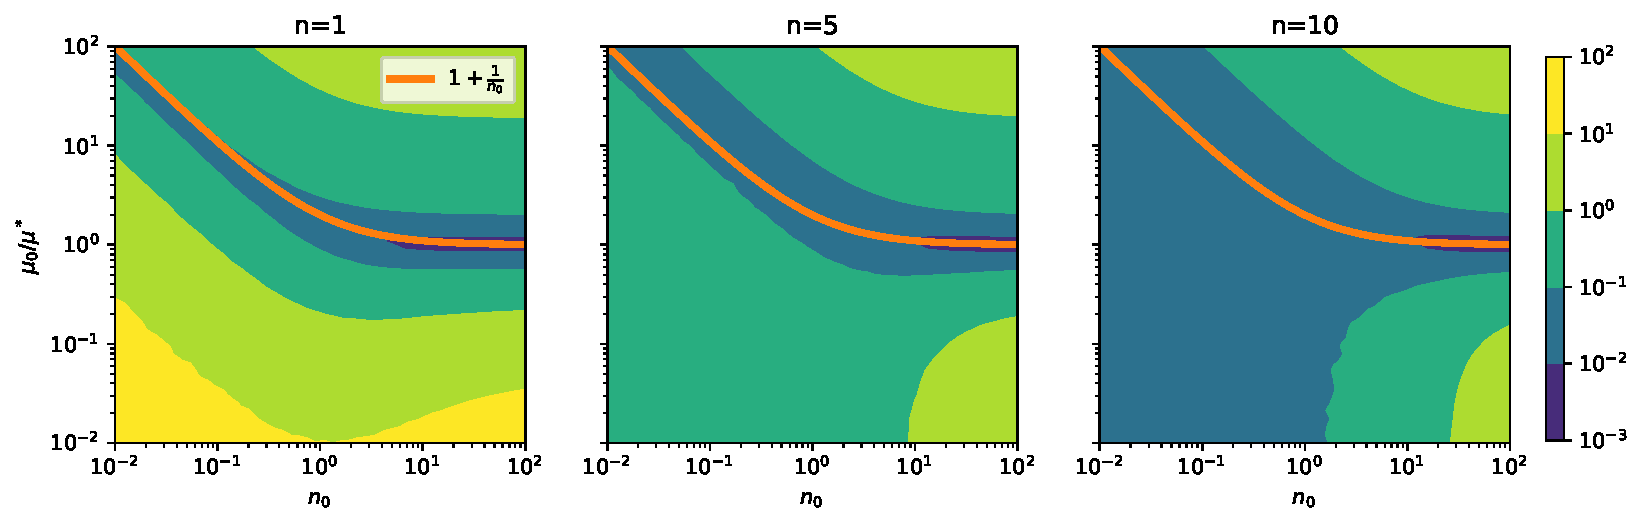
\includegraphics[width=\textwidth]{optimal_n0.pdf}
	\caption[On the optimal priors $(n_0, \mu_0)$.]{
	\textbf{On the optimal priors $(n_0, \mu_0)$.}
	Contours of $\expect{\KL(\nat^*, \hat \nat_n)}$  for the Gaussian variance with $n\in\{1,5,10\}$, $\mu^*=1$ and $n_0, \mu_0$ spanning $[10^{-2}, 10^2]$. The expectation was estimated with $10^4$ draws for each value of $n_0, \mu_0$ We observe that the line $\frac{\mu_0}{\mu^*} = 1 + \inv{n_0}$ coincides with the bottom valley of this landscape.
	}
	\label{fig:optimal_n0}
\end{figure}


\section{Complements on Gaussians}
\label{app:gaussian}

%TODO ostroskii and bach are using a subgaussian assumption which does not hold for a Gaussian, so there might still be work to do. But also check anastasiou to be sure.

In this section, we prove that for a Gaussian, the entropy and log-partition functions are self-concordant.
We also provide complementary illustrations of 
these functions in \cref{fig:logpart-entropy}, 
their gradients (e.g. the mirror maps) in \cref{fig:mirrormaps},
and paths taken by MLE and MAP in \cref{fig:gaussian-paths} .

The Gaussian log-partition function and entropy are, up to constants,
\alignn{
	\logpart(\nat) &= \frac{\nat_1^2}{-4\nat_2} - \half \log(-\nat_2) \label{eq:app-logpart} \\
	\conj(\m) &= - \half \log (\mu_2 - \mu_1^2) \; , \label{eq:app-entropy}
}
where $\nat_1\in\real, \nat_2 <0$ and $\mu_1\in\real, \mu_2>\mu_1^2$.
We provide definitions of self-concordance in \cref{app:self-concordant}.

\begin{figure}[ht]
	\centering
	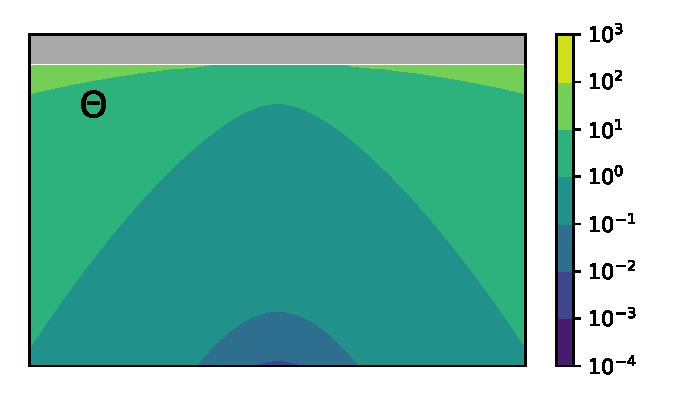
\includegraphics[width=.45\textwidth]{2d/logpart.pdf}
	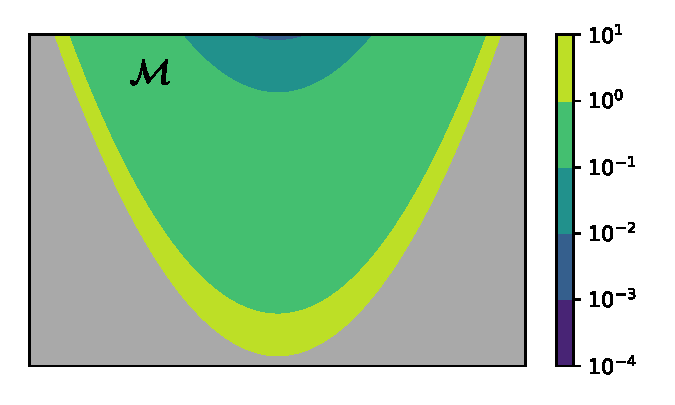
\includegraphics[width=.45\textwidth]{2d/entropy.pdf}
	\caption[Contours of the Gaussian log-partition function and entropy.]{
	(left) Contours of the log-partition function~\eqref{eq:app-logpart}.
	(right) Contours of the entropy~\eqref{eq:app-entropy}.
	}
	\label{fig:logpart-entropy}
\end{figure}

\begin{figure}[ht]
	\centering
	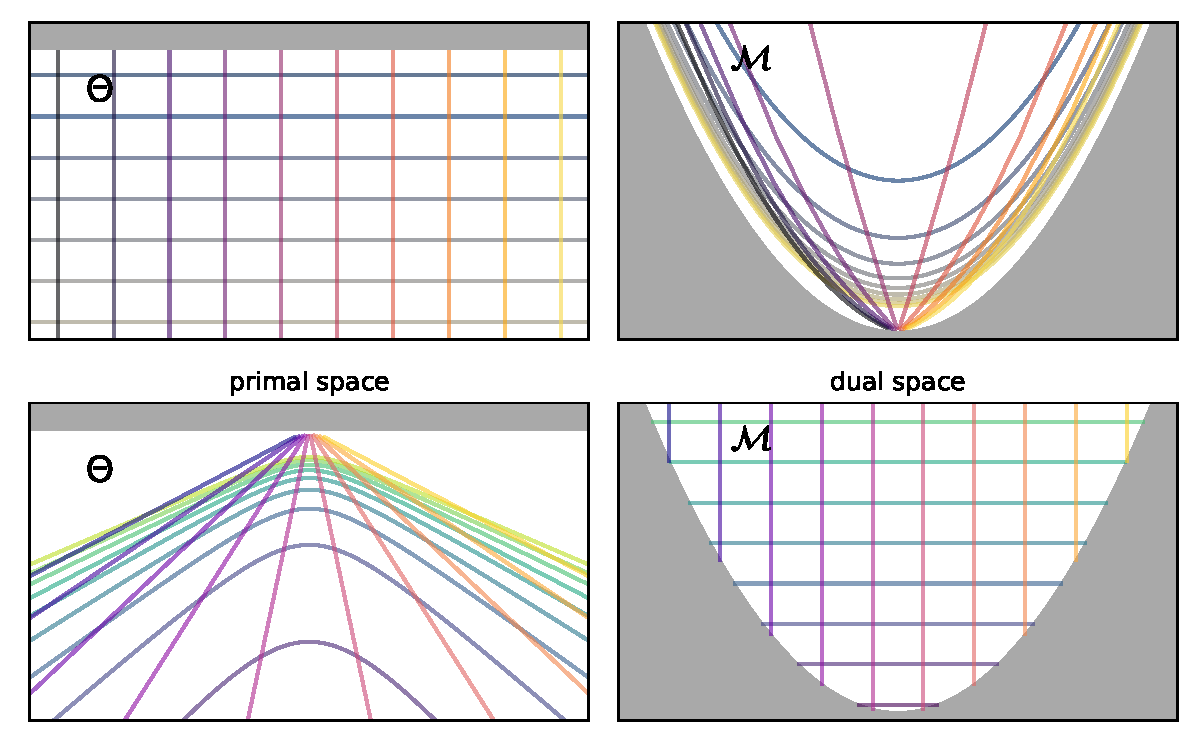
\includegraphics[width=.9\textwidth]{2d/mirrormap.pdf}
	\caption[Visualizations of the Gaussian mirror-map.]{
	\textbf{Visualizations of the Gaussian mirror-map.}
	(top) Grid deformation produce by $\nabla \logpart(\nat)$.
	(bottom) Grid deformation produced by $\nabla\conj(\m)$.
	}
	\label{fig:mirrormaps}
\end{figure}

\begin{figure}[ht]
	\centering
	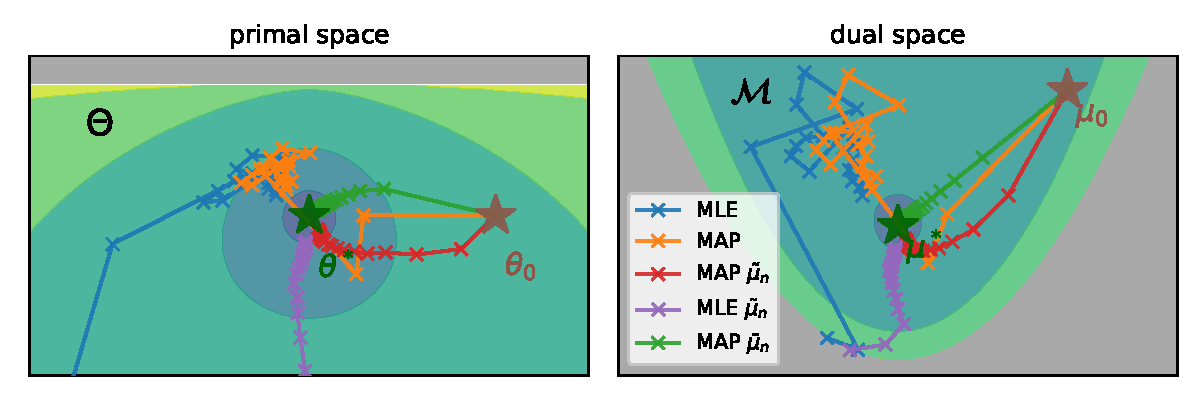
\includegraphics[width=.9\textwidth]{2d/gaussian_paths.pdf}
	\caption[MLE and MAP sample trajectories for a Gaussian.]{
		Paths taken by MLE (blue) and MAP (orange) on top of contours for $\KL(\nat^* || \nat)$. 
		We set $\mu^*=(0, 1), \mu_0 = (1, 2)$, and $n_0=4$, and $n$ varies from $1$ to $20$.
		In green, red and purple, we represent the paths respectively taken by the MAP dual expectation  $(\bar\nat_n, \bar \mu_n)$, MAP primal expectation $(\tilde\nat_n,\tilde\mu_n)$, and MLE primal expectation. Recall that the MLE dual expectation is $\mu^*$ itself.
	}
	\label{fig:gaussian-paths}
\end{figure}


\paragraph{Entropy is Self-Concordant.}
\citet[Example 4.1.1.4,   p.177]{nesterov2003introductory} proves that logarithmic barriers for second order regions are self-concordant, 
that is functions of the form 
\alignn{
	f(\theta) = -\log\paren{\alpha + \lin{a, \theta} - \frac{1}{2}\lin{\mA \theta, \theta}}
	\text{ on }
	\left\{\theta\in\mathbb{R}^n \cond \alpha + \lin{a, \theta} - \frac{1}{2}\lin{\mA \theta, \theta} > 0\right\}.
}
The entropy~\eqref{eq:app-entropy} fits into this definition with $\mA = \begin{pmatrix} 2 & 0 \\ 0 & 0 \end{pmatrix}$ and $a = ( 0 \ 1 )^\top$.

\paragraph{Log-partition is Self-Concordant.}
As proved in \citet{nesterov1994interior}, self-concordance is preserved by Fenchel conjugacy.
Since $\conj$ is self-concordant, $\logpart$ is as well.
For a more accessible reference, see also \citet[Prop.~6]{sun2019generalized}.

\section{Asymptotic Derivation}
\label{app:asymptote}
In this section we fill-in the lines of \S\ref{ssec:asymptote} to prove Equation~\eqref{eq:asymptote}.
Approximating $\conj$ with a second order Taylor expansion yields
\aligns{
    \bregmanconj(\m^* ; \m)
    &= \frac{1}{2}\norm{\m - \m^*}^2_{\mF}
    + O(\norm{\m - \m^*}^3),
}
where the norm is induced by the matrix
\aligns{
    \mF
    :=\nabla^2\conj(\m^*)
    = \nabla^2\logpart(\nat^*)^{-1}
    = \Cov_{\nat^*}(T)^{-1},
}
where the second equality is a general property of convex conjugates.
Plugging the MLE~\eqref{eq:defMLE} into this quadratic and expanding it yields
\aligns{
	\E \half \norm{\inv{n}  \sum_i T_i - \m^* }_\mF^2 
	&=\inv{2n^2} \sum_i \E \norm{T_i - \m^* }_\mF^2 
	+ \inv{2n^2} \sum_{i\neq j}\expect{T_i - \m^*}^\top \mF \overbrace{\expect{T_j - \m^*}}^{0}\\
	&=\inv{2n}  \E \norm{T_1 - \m^* }_\mF^2 \\
	& = \inv{2n} \Tr(\mF\ \expect{(T_1 - \m^*) (T_1 - \m^*)^\top}) \\
	&= \inv{2 n} \Tr(\mF \Cov_{\nat^*}(T)) = \frac{d}{2n} ,
}
where on the first line we used independence of samples, on the second line we used the fact that samples are identically distributed, and on the third line we used the  trace trick along with the linearity of the trace $\Tr$.
On the way, this also proves that for the MLE $\norm{\m - \m^*}^3 \in O(n^{-\half[3]})$.
This yield the final rate for the MLE
\begin{align}
	\E \bregmanconj \paren{\E [T(X)] ; \inv{n}  \sum_i T_i}
	= \frac{d}{2n} + O(n^{- \frac{3}{2}} ) \; .
\end{align}
For the MAP~\eqref{eq:defMAP}, the quadratic decomposes into bias and variance:
\begin{align}
	\E \half \norm{\mu^* -  \frac{n_0 \mu_0 + \smallsum_i T(x_i)}{n_0+n} }^2_{\mF}
	&= \frac{n d}{2(n+n_0)^2}  +  \frac{n_0^2}{(n+n_0)^2} \half \norm{\mu^* -  \mu_0}^2_{\mF} \\
	&= \frac{d}{2n} + O\left(\frac{1 + \norm{\mu^* -  \mu_0}^2_{\mF} }{n^2} \right) \; .
\end{align}
This $O(n^{-2})$ term is dominated by the $O(n^{-\half[3]})$ term from the quadratic approximation of the Bregman, yielding the same first order rate as for the MLE
\begin{align}
	\E \bregmanconj \paren{\E [T(X)] ; \frac{n_0 \mu_0 + \smallsum_i T(x_i)}{n_0+n} }
	= \frac{d}{2n} + O(n^{- \frac{3}{2}} ) \; .
\end{align}

\section{Self-Concordance}
\label{app:self-concordant}

In this section, we define self-concordance and we prove Proposition~\ref{prop:selfConcordant}.

\begin{definition}[Self-concordance]
\label{def:self-concordance}
A convex function is $F:\real^p \rightarrow \real$ is self-concordant if it is differentiable $3$ times and if for all $w, v \in\real^p$ the function $g(t) = F(w+tv)$ satisfies for all feasible $t$
\alignn{
	\abs{g'''(t)} \leq 2 g''(t)^{\frac{3}{2}} \; .
}
\end{definition}

%\begin{definition}[Pseudo Self-concordance] \citep{bach2010self} 
%A convex function is $F:\real^p \rightarrow \real$ is self-concordant if it is differentiable $3$ times and if for all $w, v \in\real^p$ the function $g(t) = F(w+tv)$ satisfies 
%\alignn{\abs{g'''(x)} \leq C \norm{v}_2 g''(x)}
%for all feasible $t$ and for some $C\geq 0$.
%\end{definition}

{\bf Clarification:} In the main text in Section~\ref{ssec:local-quadratic}, we claimed that the Fenchel conjugate of a 1-dimensional function is also self-concordant. 
Actually, this is also true in higher dimensions, as proved by \citet{nesterov1994interior}. See \citet[Prop.~6]{sun2019generalized} for a more accessible reference.


\subsection{Properties of Self-concordant functions}

We quickly review some important properties of self-concordant functions, introduced in \citep{nesterov2003introductory}. We start with a some notation. Let $A^*$ be a self-concordant function. Then, we write
\begin{itemize}
	\item the local norm $\|\cdot\|_x = \sqrt{ \langle \nabla^2A^*(x)\cdot,\, \cdot \rangle }$ 
	\item the distance function $\omega(t) = t-\ln (1+t),\;t\geq 0$, and its dual $\;\omega^*(t) = -t-\ln(1-t)$ defined for $t\in [0,1]$.
\end{itemize}
Note that $\omega^*(t)$ is positive, convex and monotonically increasing for $t\in[0,1]$.

\begin{figure}[ht]
	\centering
	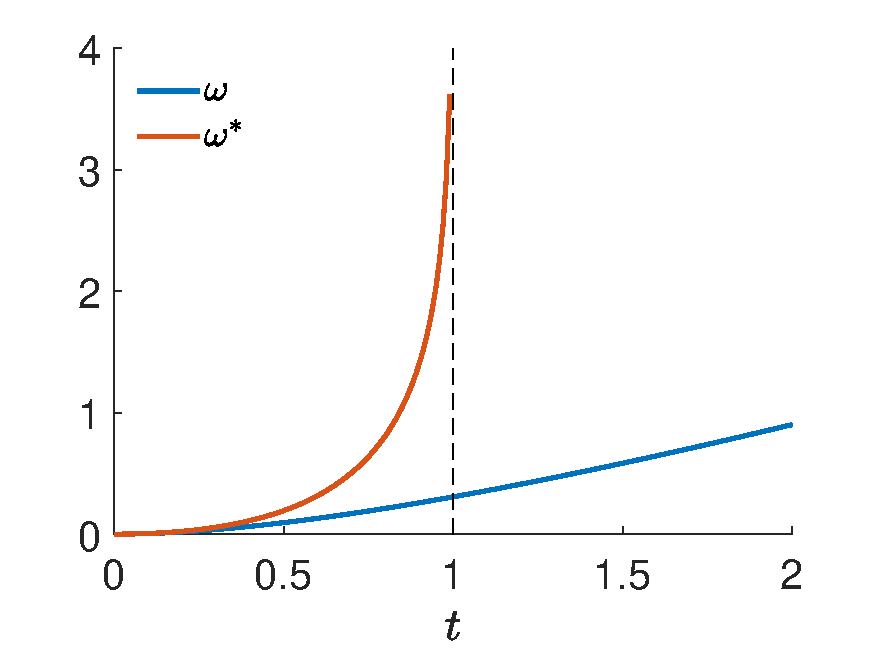
\includegraphics[width=0.4\textwidth]{self_concordance/omega.pdf}
	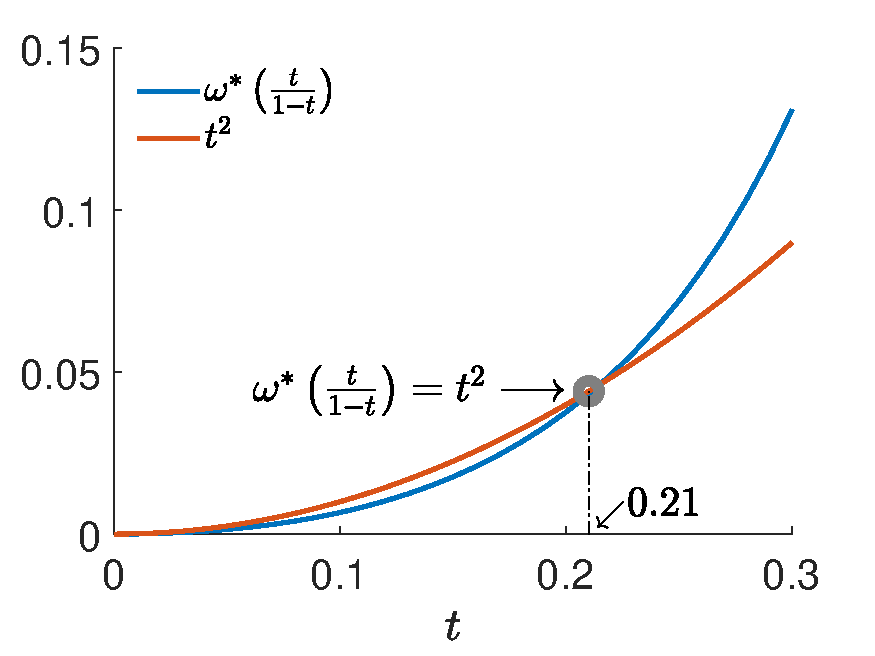
\includegraphics[width=0.4\textwidth]{self_concordance/omega_star.pdf}
	\caption[Self-concordance proof functions.]{(left) Graph of the distance function $\omega$ and its dual $\omega^*$. (right) Graph of the dual of distance function $\omega^*$ evaluated at $\frac{t}{1-t}$, compared with $t^2$. The two curves cross each other at $t\approx 0.21$.}
	\label{fig:omega}
\end{figure}

We now present two important results. The first one shows how to convert the local norm $\|y-x\|_y$ using $\|y-x\|_x$.
\begin{proposition}\label{prop:conversion_norm}
	(Conversion of norms, \citep[Theorem 4.1.5]{nesterov2003introductory}) For any $x,\,y\in\dom A^*$, if $\|y-x\|_x<1$, then
	\[
		\|y-x\|_y \leq \frac{\|y-x\|_x}{1-\|y-x\|_x}.
	\]
\end{proposition}

The next result shows that, if $y$ is sufficiently close to $x$, then we can bound the Bregman divergence of $A^*$ using the distance function $\omega^*$ and local norms.
\begin{proposition}(Upper bound of self-concordant functions \citep[Theorem 4.1.8]{nesterov2003introductory}) \label{prop:upper_bound_self_concordance}
	For any $x,\,y\in\dom A^*$, if $\|y-x\|_x<1$, then
	\[
		\bregmanconj(y,x) \leq \omega^*(\|y-x\|_x).
	\]
\end{proposition}

We are now ready to prove Proposition~\ref{prop:selfConcordant}.


\subsection{Proof of Proposition~\ref{prop:selfConcordant}.}

We start with Proposition~\ref{prop:upper_bound_self_concordance}, evaluated at $y=\meanp^*$ and $x=\meanp$:
\[
	\bregmanconj(\meanp^*,\meanp) \leq \omega^*(\|\meanp^*-\meanp\|_{\meanp}).
\]
This hold if $\|\meanp^*-\meanp\|_{\meanp}<1$. Since $\omega^*$ is monotonically increasing, we can replace $\|\meanp^*-\meanp\|_{\meanp}$ by its upper bound from Proposition~\ref{prop:conversion_norm},
\[
	\omega^*(\|\meanp^*-\meanp\|_{\meanp}) \leq \omega^*\left(\frac{\|\meanp^*-\meanp\|_{\meanp^*}}{1-\|\meanp^*-\meanp\|_{\meanp^*}}\right),
\]
under the conditions that $\|\meanp^*-\meanp\|_{\meanp^*}<1$ (to satisfy the assumption of Proposition~\ref{prop:conversion_norm}) and $\frac{\|\meanp^*-\meanp\|_{\meanp^*}}{1-\|\meanp^*-\meanp\|_{\meanp^*}} <1$ (to ensure that $\|\meanp^*-\meanp\|_{\meanp} <1$). Those two conditions holds if $\|\meanp^*-\meanp\|_{\meanp^*} <0.5$. Now, we use the bound (see figure \ref{fig:omega})
\[
	\omega^*\left(\frac{t}{1-t}\right) \leq t^2, \quad 0\leq t \leq 0.21,
\]
and replace $t$ by $\|\meanp^*-\meanp\|_{\meanp^*}$. This finally gives the sequence of inequalities
\[
	\bregmanconj(\meanp^*,\meanp) \leq \omega^*(\|\meanp^*-\meanp\|_{\meanp}) \leq \omega^*\left(\frac{\|\meanp^*-\meanp\|_{\meanp^*}}{1-\|\meanp^*-\meanp\|_{\meanp^*}}\right) \leq \|\meanp^*-\meanp\|_{\meanp^*}^2,
\]
that holds while $ \|\meanp^*-\meanp\|_{\meanp^*}<0.21$, which is the desired result.



\section{Bias-Variance}
\label{app:bias-variance}
In this section, we start from the notions of bias and variance introduced in \cref{eq:bias-variance}.
First, we prove that the bias of the MLE of a Gaussian variance decreases in $O(\inv{n^2})$. 
Then we prove that assuming~\eqref{eq:hanzely} holds, whether uniformly or in expectation, yields a convergence rate on the variance term.

\subsection{Bias of a Gaussian Variance MLE}
For a Gaussian variance model, the MLE follows a scaled $\chi^2(n)$ distribution. 
This means that
\alignn{
	\frac{\m^*}{\tilde \m_n} 
	= \frac{\tilde\nat_n}{\nat^*}
	=\expect{\frac{\hat\nat_n}{\nat^*}}
	=\expect{\frac{\m^*}{\hat \m_n} }
	=\expect{\frac{n}{\chi^2(n)}}
	= \frac{n}{n-2}\; .
}
Consequently,
\alignn{
	\bregmanconj(\m^*, \tilde \m_n) 
	&= \half \paren{\frac{n}{n-2} -1 + \log\frac{n-2}{n}}\\
	&= \frac{1}{n-2} + \half \log\paren{1 - \frac{2}{n}}\\
	&\leq \inv{n-2} - \inv{n} 
	= \frac{2}{n(n-2)},
}
so the bias of the MLE of a Gaussian Variance decreases like $O\paren{\inv{n^2}}$.

\subsection{Expectation of SMD's Variance Assumption}
The first step is to notice the symmetrized Bregman can be expressed as an inner product between primal and dual parameters
\alignn{
	\cS_\conj (\mu , \bar\mu)
	= \lin{ \nabla \conj(\mu) - \nabla \conj(\bar\mu) , \mu - \bar\mu}
	= \lin{ \nat -\bar\nat , \mu - \bar\mu} \; .
}
Now notice that~\eqref{eq:hanzely} features $\mu := \hat \mu_{n+1} = \hat\m_{n} - \stepsize g(\hat \nat_{n})$ stochastic and $\bar\mu := \bar\mu_{n+1} =  \hat\m_{n}   -\stepsize \nabla f(\hat \nat_{n})$ deterministic such that $\E_g[\mu] = \bar\mu$.
For such a pair of variables, the expectation of the symmetrized Bregman corresponds to a covariance between primal and dual parameters
\alignn{
	\expect{\cS_\conj (\mu , \E[\mu])} 
	= \expect{\lin{\nat, \mu - \E[\mu]}}
	= \underbrace{\expect{\lin{\nat, \mu}} -\lin{\expect{\nat}, \expect{\mu} } }_{\Cov(\nat, \mu)}
	=\expect{\lin{\nat - \E[\nat],\mu}} 
	= \expect{\cS_\logpart(\nat, \E[\nat])} \; .
}
The last equality holds by symmetry between the roles of $\logpart$ and $\conj$.
Note that the middle covariance formulation is actually the one  used by \citet{hanzely2018fastest}.
Now, \cref{eq:bias-variance} defines the variance as 
\alignn{
	\expect[1:n]{\bregmanconj(\tilde \m_n , \hat\m_n) }
	=\expect[1:n]{\bregman(\hat\nat_n , \E_{1:n}[\hat\nat_n]) }
	\leq \expect[1:n]{\cS_A(\hat\nat_n , \E_{1:n}[\hat\nat_n]) }
	=  \expect[1:n]{\cS_\conj(\hat\mu_n , \E_{1:n}[\hat\mu_n]) }\;,
	\label{eq:bregman-covariance}
}
where expectations $\E_{1:n}$ are on all samples $X_1, \dots, X_n$, whereas~\eqref{eq:hanzely} is written with 
\alignn{
	\expect[n]{\cS_\conj(\hat\mu_n , \E_{n}[\hat\mu_n]) } \leq \stepsize^2 C \; ,
}
where the expectation $\E_{n}$ is taken over only the last sample $X_n$, and the bound should hold uniformly over all $\hat\mu_{n-1}$.
Taking the expectation over $\hat\mu_{n-1}$ instead gives
\alignn{
	\expect[1:n]{\cS_\conj(\hat\mu_n , \E_{n}[\hat\mu_n]) }  \leq \stepsize^2 C \;.
}
The only difference with the right hand side of \cref{eq:bregman-covariance} is in the inner expectation.
To overcome this difference, we need to plug in the form of $\hat \mu_n = \frac{n_0\mu_0 + \sum_i T_i}{n_0 +n}$. Notice that 
\alignn{
	&\MAPm - \E_n[\MAPm] = \frac{T_n - \m^*}{n_0+n} \\
	\implies & \expect[1:n]{\cS_\conj(\hat\mu_n , \E_{n}[\hat\mu_n]) }
	= \inv{n_0+n} \expect[1:n]{ \lin{\MAPt , T_1 - \m^*} },
}
while
\alignn{
	&\MAPm - \E_{1:n}[\MAPm] = \frac{\smallsum_i (T_i - \m^*)}{n_0+n} \\
	\implies & \expect[1:n]{\cS_\conj(\hat\mu_n , \E_{1:n}[\hat\mu_n]) }
	=\frac{n}{n_0+n} \expect[1:n]{ \lin{\MAPt , T_1 - \m^*} } \; .
}
In the end, we get that the variance is dominated by $n$ times the expectation of \cref{eq:hanzely}:
\alignn{
	\expect[1:n]{\bregmanconj(\tilde \m_n , \hat\m_n) }
	\leq n \expect[1:n]{\cS_\conj(\hat\mu_n , \E_{n}[\hat\mu_n]) }  \; .	
}
If assumption~\eqref{eq:hanzely} holds, then we have
\alignn{
\expect[1:n]{\bregmanconj(\tilde \m_n , \hat\m_n) }
\leq n \stepsize_n^2 C \in O\paren{\inv{n}} \; ,
}
where we assumed $\stepsize_n  \in O\paren{\inv{n}}$.
In conclusion, assuming~\eqref{eq:hanzely} holds uniformly or in expectation immediately implies a $O\paren{\inv{n}}$ convergence rate on the variance.




\section{Review of SMD}
\label{app:SMD}

We use this section to give more details on the (stochastic) mirror descent algorithm.
We start with gradient descent with step-sizes $\gamma$. 
the update $\theta_{n+1} = \theta_n - \gamma \nabla f(\theta_n)$ can be viewed as the minimization of the linear approximation of $f$ at $\theta_n$
$f(\theta) \approx f(\theta_n) + \lin{\nabla f(\theta_n), \theta - \theta_n}$, 
alongside with quadratic penalty scaled by ${1}/{\gamma}$:
\alignn{
	\theta_{n+1} = \arg\min_\theta f(\theta_n) + \lin{\nabla f(\theta_n), \theta - \theta_n} + \frac{1}{\gamma} \frac{1}{2}\norm{\theta - \theta_n}^2.
}
Mirror descent generalizes the above, using the Bregman divergence induced by a (Legendre) function $A$ instead of the Euclidean norm as follow, 
\alignn{\label{eq:mirror-descent-primal}
	\theta_{n+1} = \arg\min_\theta f(\theta_n) + \lin{\nabla f(\theta_n), \theta - \theta_n} + \frac{1}{\gamma} \bregman(\theta, \theta_n).
}
Mirror descent coincides with gradient descent if $A(\theta) = \frac{1}{2}\norm{\theta}^2$.
As \cref{eq:mirror-descent-primal} is convex, the minimum is at a stationary point, 
found by taking the derivative and setting to 0, 
leading to the update $\theta_{n+1}$ satisfying
\alignn{
	\nabla f(\theta_n) + \frac{1}{\gamma}\paren{\nabla A(\theta_{n+1}) - \nabla A(\theta_n)} = 0
	&&\implies&&
	\nabla A(\theta_{n+1}) = \nabla A(\theta_n) - \gamma \nabla f(\theta_n).
}
Expressed with the dual parameters, we obtain $\mu_{n} = \nabla A(\theta_{n})$, 
$\mu_{n+1} = \mu_n - \gamma \nabla f(\theta_n)$. 

{\bf In our case,} where the objective function is the (negative) log-likelihood of an exponential family, we have
\alignn{
	f(\theta) = A(\theta) - \lin{\frac{1}{n} \sum_{i=1}^n T(X_i), \theta}.
}
Using Mirror descent with a step-size of $1$ and the log-partition function $A$ as the reference function gives
\alignn{\begin{aligned}
	\mu_{n+1} 
	= \mu_n - \nabla f(\theta_n)
	= \mu_n - \paren{\nabla A(\theta_n) - \frac{1}{n}\sum_{i=1}^n T(x_i)}
	= \frac{1}{n}\sum_{i=1}^n T(x_i).
	\end{aligned}
}
In a stochastic, online version 
where the linearization of the objective is obtained from iid samples, 
a decreasing step-size of $\gamma_n = 1/n$ recovers the ``online'' estimate of the MLE.
The case of $\mu_1 = T(x_1)$ follows from the above, 
and in general, assuming it holds for $\mu_n$, 
\alignn{\begin{aligned}
	\mu_{n+1} &= \mu_n - \gamma_n g(\theta_n)
	= \mu_n - \gamma_n (\mu_n - x_n)
	\\
	&= (1 - \frac{1}{n}) \mu_n + \frac{1}{n} T(x_n)
	=
	\frac{n-1}{n} \frac{1}{n-1}\sum_{i=1}^{n-1} T(x_i)
	= 
	\frac{1}{n} \sum_{i=1}^{n} T(x_i)
	+ \frac{1}{n} T(x_n).
\end{aligned}}
The derivation in the main text gives the more general result, 
of using step-sizes of the form $1/(n+n_0)$ to recover online MAP estimation 
with a conjugate prior depending on $n_0$ and the initial estimate of the parameters $\theta_0$.

	
\end{subappendices}




\iffalse
\section{TODO}
\begin{enumerate}
	\item new plots: add 2d trajectories to paper, with background level set, and new legend: primal/dual expectation, and clear explanation!
	\item Incorporate related work by Frederik.
	\item Technical Background: be precise and add a reference for the steep exponential family of Legendre type, which guarantees that our sets are open and have a solution in the middle.
	References: \begin{itemize}
		\item \href{https://www.jstor.org/stable/4616462?seq=1#metadata_info_tab_contents}{Existence of Maximum Likelihood Estimates for Multi-Dimensional Exponential Families},
		\item The singly truncated normal distribution: A non-steep exponential family,
		\item Statistical exponential families: A digest with flashcards,
		\item Information and Exponential Families In Statistical Theory,
		\item Fundamentals of Statistical Exponential Families with Applications in Statistical Decision Theory.
	\end{itemize}
\end{enumerate}




\section{Blurbs/ideas?}



\subsection{SGD blurb}
\fdk{
%
There is a long line of work bounding the convergence rate of stochastic gradient descent.
Beyond the results of \citet{robbins1951stochastic},
we now have proofs on smooth, strongly convex problems and bounded variance
(as well as other assumptions on the noise, reviewed later)
a decreasing step-size and an averaging scheme gets
a $1/t$ convergence rate,
which matches the asymptotic rate of unbiased estimation,
through clever averaging schemes \citep{rakhlin2012making,lacostejulien2012simpler}
\\
Those papers assume the stochastic gradients are bounded,
but minor modifications also work for bounded variance instead.
\\
We do have extensions to other notions of bounded variance,
for example, assuming that the stochastic gradients are gradients of a perturbed smooth function $f_i$
and that the minimum of $f$ and the minima of the $f_i$
are bounded, $\expect{\min_x f(x) - \min_x f_i(x)} \leq \sigma^2$,
or that the gradient noise is bounded only at the minimum.
For a review, see \citet{gower2019sgd}.
\\
However, for some problems, combining decreasing step-sizes and averaging is not necessary,
even when the function is not strongly convex.
This is the case for maximum likelihood estimation and matches the asymptotic rates,
but holds more generally, for example, for linear and logistic regressions \citep{bach2013nonstronglyconvex,moulines2011non}.
}


\subsection{Poisson likelihood?}
\fdk{
\citet{bauschke2017descent} and \citet{hanzely2018fastest} both use the example of Poisson inverse problems/Poisson regression
as examples.
The simpler case of the MLE of a Poisson distribution is also unsolved, though.
In this case, $h(x) = 1/x!$, $x \in \mathbb{N}$, $A(\theta) = e^\theta$ over $\theta \in \mathbb{R}$,
$A^*(\m) = \m \log \m - \m$ over $\m \in \mathbb{R}_+$.
It is neither strongly-convex nor self-concordant (at least according to the standard definition,
although it satisfies generalized notions of self-concordance as $A'''(\theta) = A''(\theta)$).
}

\subsection{``simple'' open problem?}
\fdk{
A ``simple open problem'';
assume we have a deterministic problem so that we know where the minimum is.
Can we figure out a (deterministic) path from $\theta_0$ to $\theta_*$
that has optimality decreasing as $1/n^2$,
to mirror the bias term of gradient descent?
}

\subsection{Connection with acceleration?}
\fdk{
The problems on how to deal with Bregman divergences abound in optimization, beyond stochasticity.
For example, we have not yet figured out the analog of Nesterov-type acceleration
on relatively smooth and strongly convex problems
to bring the convergence rate from linear in $(1-\kappa)$ to $(1-\sqrt{\kappa})$,
or just from $1/T$ to $1/T^2$ in the (non-strongly) convex case.
\citet{dragomir2021optimal}  shows that naïve application of Bregman updates can not achieve acceleration.
The tools developed to make progress on one problem might help make progress on the other.
}






\newpage
\section{Notation convention}
We use
\begin{itemize}
	\item $\theta, \nat$ for natural parameters
	\item $\m$ for mean parameters
	\item $X_1,\ldots,X_n$ for data
	\item $\cX$ for the data space
	\item $T$ for the sufficient statistics
	\item $\nu$ for the base measure
	\item $A, A^*, \logpart, \conj$ for the log-partition and its dual
	\item $\cB_A$ for the Bregman divergence induced by $A$
	\item $n$ for the number of samples
	\item $(\theta^*,m^*)$ for the optimum
	\item $\gamma, \stepsize$ for the step-size
	\item $\mu,\sigma^2$ for the parameters of a Gaussian
	\item $\hat\theta_n$ for estimates
	\item $\tilde\theta_n$ for $\expect{\hat\theta_n}$, which is biased
	\item $(\stgcvx , \smooth)$ for strong-convexity and smoothness
\end{itemize}
\fi


\chapter{Conclusion}
\label{chap:discussion}

The three contributions of this thesis deal with the interweaved topics of optimization and statistics. 
These three contributions can be summarized as 
\begin{enumerate}
	\item Variance reduction allows fast training of CRF, a particular class of conditional undirected graphical models that were previously hard to optimize. Thanks to duality, non-uniform sampling can be elegantly formalized and improved other strong methods.
	\item For some simple classes of models, the causal model is faster to adapt to interventions than the anticausal one only when the intervention bears on the cause. 
	However, our intuitions dictate that causal models should have some real-world advantages compared to non-causal ones. 
	That may be why humans learn new rules so quickly.
	We may need more sophisticated models to instantiate this intuition in machine learning.
	\item The maximum likelihood estimate of an exponential family can also be seen as the output of stochastic mirror descent. Furthermore, the KL divergence between the true and learned models is simply a Bregman divergence. Nevertheless, neither optimization nor statistics communities have found upper bounds on this quantity that apply to any sample size and families such a Gaussians. 
	Finding such an upper bound may help non-Euclidean optimization reach new grounds.
\end{enumerate}
This last contribution reveals that while exponential families are at the core of most machine learning techniques, some of their properties are yet to be understood.
Throughout this thesis, we alternated between optimization and statistics perspectives, displaying the synergy between these two fields. Thanks to optimization tools, statistical models are becoming more powerful. Thanks to statistical models, we can probe into the abilities of optimization methods.


\section{Future Work}
Based on our last contribution, we identify two promising research directions.
\begin{enumerate}
	\item finding high probability bounds for exponential family MAP thanks to the entropy being a self-concordant barrier, as proved by \citep{bubeck2015entropic}.
	That would provide a general large sample result. A low sample result remains to be found.
	\item Analyzing the convergence properties of stochastic mirror descent on self-concordant (barrier) losses. This might be possible thanks to the quadratic sandwich property of such functions, and it might be possible to find a high probability convergence rate. 
\end{enumerate}
These research directions may help us understand fundamentals statistical models and design better stochastic optimization methods for objectives that are Legendre functions.


 % S'il y a une bibliographie pour tout le document, on peut
 % utiliser les commandes suivantes. À noter que le style est
 % laisser au choix de l'auteur·e. (Il est même possible
 % d'utiliser <natbib>).
 % Il est possible d'avoir une bibliographie pour chaque
 % chapitre. Consulter l'article en exemple pour voir
 % comment faire.
%  \chapter*{References}
\bibliographystyle{abbrvnat}
%\bibliography{references}
\bibliography{references1,references2,references3}

\end{document}
